\label{chapter:introcomp}
Este capítulo tiene por objeto darte una visión global de la 
estructura de un compilador e introducirte en las técnicas básicas
de la construcción de compiladores usando Perl.

Puesto que no todos los alumnos que se incorporan en este capítulo 
han leído los anteriores y no necesariamente conocen Perl, en la sección
\ref{section:lasbases}
comenzamos haciendo un breve repaso a como construir un módulo en Perl.
Si quieres tener un conocimiento mas profundo
lee el capítulo sobre módulos en 
\eref{chapter:modulos}. 

La sección 
\ref{section:fases}
describe las fases en las que -al menos conceptualmente-
se divide un compilador.
A continuación la sección 
\ref{section:analisislexico}
presenta la primera de dichas fases, el análisis léxico.
En la sección 
\ref{section:conceptos}
repasamos conceptos de análisis sintáctico 
que deberían ser familiares a cualquiera que haya 
seguido un curso en teoría de autómatas 
y lenguajes formales.
Antes de comenzar a traducir es conveniente tener un \emph{esquema} o estrategia
de traducción para cada constructo sintáctico. 
La sección 
\ref{section:esquemas}
introduce el concepto de esquema de traducción.
La fase de análisis sintáctico consiste en la construcción
del \emph{árbol de análisis} a partir de la \emph{secuencia de unidades léxicas}. 
Existen diversas estrategias para resolver esta fase.
En la sección 
\ref{section:predictivo}
introducimos la que posiblemente sea la mas sencilla de todas: el análisis
descendente predictivo recursivo.
En la sección
\ref{section:recursionizquierda}
abordamos una estrategia para transformar ciertas
gramáticas para las que dicho método no funciona.

Un analizador sintáctico implícitamente construye 
el árbol de análisis concreto. En muchas ocasiones
resulta mas rentable trabajar con una forma simplificada
(\emph{abstracta}) del árbol que contiene la misma información 
que aquél. La sección 
\ref{section:aat} trata de la construcción de los 
árboles de análisis abstractos.

\section{Las Bases}
\label{section:lasbases}
Puesto que no todos los alumnos que están interesados en esta sección
tienen conocimientos previos de Perl, en esta sección
comenzamos haciendo un breve repaso a como construir un módulo en Perl
y al mismo tiempo repasamos las características usadas del lenguaje.
Si quieres tener un conocimiento mas profundo
de como construir un módulo, lee el capítulo
sobre módulos en \eref{chapter:modulos}.

\parrafo{Version}

El comportamiento de Perl puede variar ligeramente si la versión que tenemos instalada es 
antigua. Para ver la versión de Perl podemos hacer.

\begin{verbatim}
lhp@nereida:~/Lperl/src/topdown/PL0506$ perl -v

This is perl, v5.8.4 built for i386-linux-thread-multi

Copyright 1987-2004, Larry Wall

Perl may be copied only under the terms of either the Artistic License or the
GNU General Public License, which may be found in the Perl 5 source kit.

Complete documentation for Perl, including FAQ lists, should be found on
this system using `man perl' or `perldoc perl'.  If you have access to the
Internet, point your browser at http://www.perl.com/, the Perl Home Page.
\end{verbatim}

\parrafo{h2xs}

En primer lugar, construimos la estructura para nuestro proyecto de mini-lenguaje.
La mejor forma de comenzar a escribir un módulo es usando la herramienta Perl
\verb|h2xs|. Supongamos que queremos construir un módulo \verb|PL::Tutu|. 
Los nombres de los módulos siguen un esquema de identificadores separados
por una pareja de \verb|:|. Para saber más sobre el esquema de nombres 
de los módulos y la forma en la que estos se asigna a ficheros del sistema 
operativo, lea la sección 
sobre introducción a los módulos \eref{section:introamodulos}.

\begin{verbatim}
lhp@nereida:~/Lperl/src/topdown/PL0506$ h2xs -XA -n PL::Tutu
Defaulting to backwards compatibility with perl 5.8.4
If you intend this module to be compatible with earlier perl versions, please
specify a minimum perl version with the -b option.

Writing PL-Tutu/lib/PL/Tutu.pm
Writing PL-Tutu/Makefile.PL
Writing PL-Tutu/README
Writing PL-Tutu/t/PL-Tutu.t
Writing PL-Tutu/Changes
Writing PL-Tutu/MANIFEST
\end{verbatim}
La herramienta \verb|h2xs| fué concebida para ayudar en la transformación
de ficheros de cabecera de C en código Perl. La opción 
\verb|-X| hace que se omita la  creación de subrutinas externas (\verb|XS|)
La opción \verb|-A| implica que el módulo no hará uso del \verb|AutoLoader|.
La opción \verb|-n| proporciona el nombre del módulo.
La llamada a \verb|h2xs| crea la siguiente estructura de directorios y ficheros:
\begin{verbatim}
lhp@nereida:~/Lperl/src/topdown/PL0506$ tree
.
`-- PL-Tutu
    |-- Changes
    |-- MANIFEST
    |-- Makefile.PL
    |-- README
    |-- lib
    |   `-- PL
    |       `-- Tutu.pm
    `-- t
        `-- PL-Tutu.t

4 directories, 6 files
\end{verbatim}

\parrafo{Generación del Makefile}

Después de esto tenemos un módulo ''funcional'' que no hace nada.
Lo podríamos instalar como si lo hubieramos descargado desde CPAN
(Véase \eref{section:instalacionamano}).

Después cambiamos al directorio \verb|PL-Tutu/| y hacemos \verb|perl Makefile.PL|.
\begin{verbatim}
lhp@nereida:~/Lperl/src/topdown/PL0506$ cd PL-Tutu/
lhp@nereida:~/Lperl/src/topdown/PL0506/PL-Tutu$ perl Makefile.PL
Checking if your kit is complete...
Looks good
Writing Makefile for PL::Tutu
\end{verbatim}
Esto crea el fichero \verb|Makefile| necesario para actualizar 
nuestra aplicación. Para saber más sobre \verb|perl Makefile.PL|
lea \eref{section:construccion}.

\parrafo{Documentación}

Pasamos ahora a trabajar en el módulo. Primero escribimos
la parte relativa a la documentación. Para ello 
editamos \verb|Tutu.pm|:
\begin{verbatim}
lhp@nereida:~/Lperl/src/topdown/PL0506/PL-Tutu/lib/PL$ pwd
/home/lhp/Lperl/src/topdown/PL0506/PL-Tutu/lib/PL
lhp@nereida:~/Lperl/src/topdown/PL0506/PL-Tutu/lib/PL$ ls -l
total 4
-rw-r--r--  1 lhp lhp 2343 2005-09-28 11:16 Tutu.pm
\end{verbatim}
y al final del mismo insertamos la documentación. Para saber más sobre el 
lenguajes de marcas de Perl (\emph{pod} por \emph{plain old documentation})
lea \eref{section:pod}. En este caso escribimos:
\begin{verbatim}
1;
__END__

=head1 NOMBRE

PL::Tutu - Compilador para un lenguaje sencillo denominado
          "Tutu" que usaremos en la asignatura PL

=head1 SINOPSIS

  use PL::Tutu;
  
  La subrutina PL::Tutu::compiler recibe dos argumentos: el 
  nombre del fichero de entrada (fuente.tutu) y el nombre del fichero de
  salida (código ensamblador para una especie de P-máquina).

=head1 DESCRIPCIÓN

Este módulo tiene dos objetivos: aprender a hacer un pequeño compilador
y aprender a programar modularmente en Perl, usando un buen número
de los recursos que este lenguaje ofrece.

El siguiente es un ejemplo de código fuente tutu:
 
  int a,b; 
  string c;
  a = 2+3;
  b = 3*4; 
  c = "hola"; 
  p c; 
  c = "mundo"; 
  p c; 
  p 9+2; 
  p a+1; 
  p b+1

supuesto que está guardado en el fichero "test2.tutu", podemos 
escribir un programa Perl "main.pl" para compilarlo: 

    $ cat main.pl
    #!/usr/bin/perl -w -I..
    #use PL::Tutu;
    use Tutu;

    PL::Tutu::compiler(@ARGV);

al ejecutar "main.pl":

    $ ./main.pl test2.tutu test2.ok

obtenemos el fichero "test2.ok" con el ensamblador: 
    $ cat test2.ok
    DATA holamundo
    PUSH 5
    PUSHADDR 0
    STORE_INT
    PUSH 12
    PUSHADDR 1
    STORE_INT
    PUSHSTR 0 4
    PUSHADDR 2
    STORE_STRING
    LOAD_STRING 2
    PRINT_STR
    PUSHSTR 4 5
    PUSHADDR 2
    STORE_STRING
    LOAD_STRING 2
    PRINT_STR
    PUSH 11
    PRINT_INT
    LOAD 0
    INC
    PRINT_INT
    LOAD 1
    INC
    PRINT_INT

Para mas información consulta la página de la asignatura.
¡Buena suerte!

=head2 EXPORT

No se exporta nada al espacio de nombres del cliente.


=head1 AUTOR

Casiano Rodríguez León, E<lt>casiano@ull.esE<gt>

=head1 VÉASE TAMBIÉN

L<perl>.

=cut
\end{verbatim}
La documentación puede ser mostrada utilizando el comando \verb|perldoc|.

\begin{latexonly}
Veáse la figura \ref{fig:perldoc}.

\begin{figure}[htb]
%\centerline{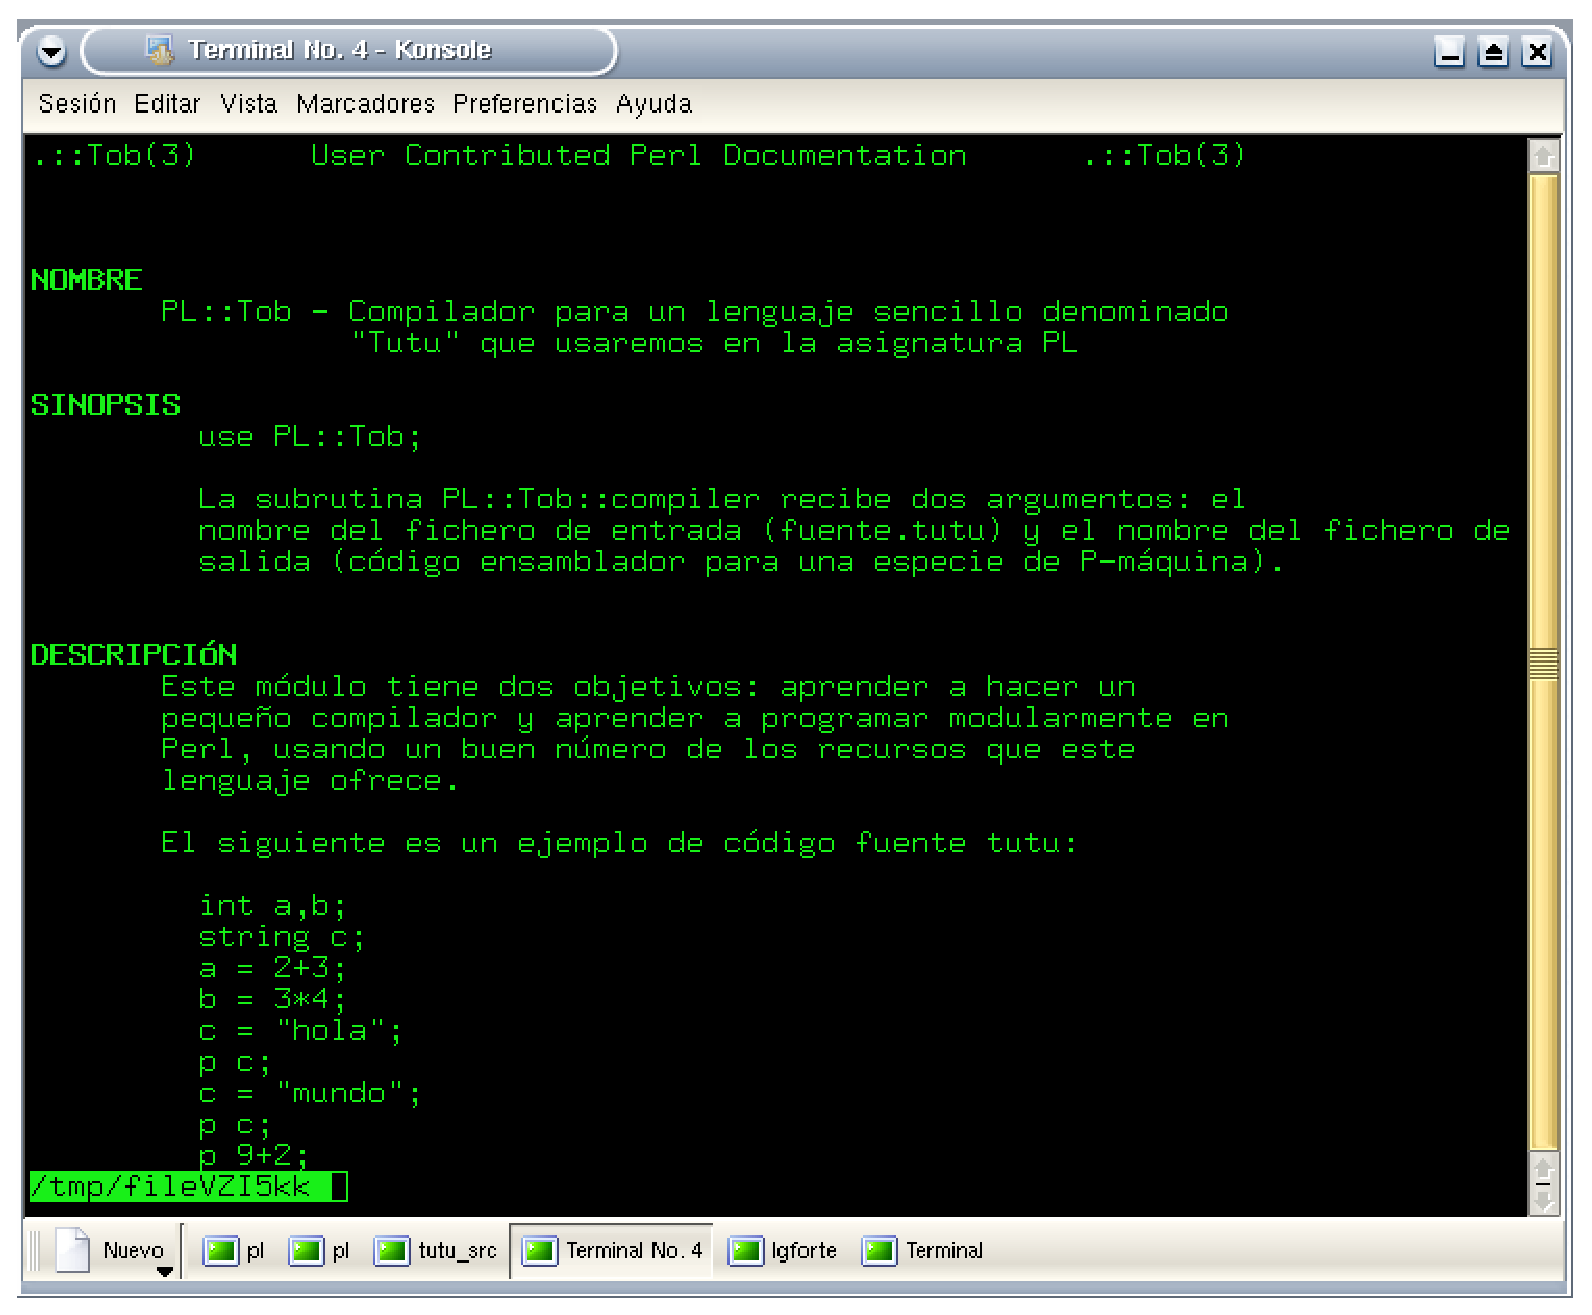
\epsfig{file=figures/perldoc.eps, height=14cm}}
\caption{El resultado de usar {\tt perldoc Tutu}}
\label{fig:perldoc}
\end{figure}
\end{latexonly}

\begin{rawhtml}
<center>
<img src="perldoc.jpg">
<p>
El resultado de usar <tt>perldoc Tutu</tt>
</center>
<hr>
<p>
\end{rawhtml}


La forma en la que se controla la calidad de un módulo es mediante 
el desarrollo de pruebas. Las pruebas son programas perl que se sitúan en el directorio
\verb|t/| y que tienen la extensión \verb|.t|. Para ejecutar las pruebas
se escribe:

\begin{verbatim}
make test
\end{verbatim}

Vease la sección \eref{subsection:laspruebas} de los apuntes de LHP para ams detalles.

\subsectionrepaso{Las Bases}
\label{repaso:lasbases}

Responda a las siguientes preguntas:

\begin{enumerate}
\item
¿Cómo puedo saber con que versión de Perl estoy trabajando?
\item
Cuando el intérprete Perl encuentra una sentencia 
\begin{verbatim}
use Este::Modulo;
\end{verbatim}
¿Donde busca el fichero \verb|Modulo.pm|?
\item
¿Con que opción debo usar Perl para ejecutar un programa en la línea de comandos?
\item
¿Cómo se llama el programa que me permite crear el esqueleto 
para una distribución de un módulo? ¿Con que opciones debo llamarlo?
\item
Cuando se crea con \verb|h2xs| el esqueleto para \verb|PL::Tutu|:
¿En que subdirectorio queda el fichero conteniendo el esqueleto del
módulo creado \verb|Tutu.pm|?
\item
¿Cuál es la función de \verb|MANIFEST|?
\item
¿Qué es \verb|Makefile.PL|? ¿Cuál es su función?
¿Que significa la frase \emph{looks good}?
\item
¿Con que comando se crea el \verb|Makefile| para trabajar en la plataforma
actual?
\item
¿Cómo se puede ver la documentación de un módulo?
\item 
¿Que hacen los siguientes comandos \verb|pod|?
Repase 
\eref{subsection:comandodeparrafo}
si tiene dudas.
\begin{verbatim}
=head1 cabecera 
=head2 cabecera 
=item texto
=over N
=back
=cut
=pod
=for X
=begin X
=end X
\end{verbatim}
\item
¿Que secuencia de comandos conocida como
\emph{mantra de instalación} es necesario ejecutar para 
instalar un módulo?
\item
¿Cual es la función del directorio \verb|t|?
\item
¿Que tipo deben tener los programas de prueba para que
\verb|make test| los reconozca como pruebas?

\end{enumerate}

\subsectionpractica{Crear y documentar el Módulo {\tt PL::Tutu}}
\label{practica:creacionydocdemodulo}
Reproduzca los pasos explicados en la sección 
\ref{section:lasbases} creando el módulo {\tt PL::Tutu}
y documentándolo. 
\begin{itemize}
\item
Compruebe que la documentación se muestra correctamente
\item
Compruebe que puede crear una distribución haciendo \verb|make dist|
\item
Compruebe que la distribución creada puede instalarse correctamente
siguiendo las instrucciones en 
\eref{section:instalacionamano}.
\end{itemize}

\section{Las Fases de un Compilador}
\label{section:fases}
La estructura del compilador, descompuesto en fases, queda explicitada 
en el código de la subrutina \verb|compile|:

\parrafo{Esquema del Compilador}

\begin{verbatim}
 1 package PL::Tutu;
 2 use 5.008004;   # Versión mínima de Perl 5.84
 3 use strict;     # Variables deben ser declaradas, etc.
 4 use warnings;   # Enviar warnings
 5 use IO::File;
 6 use Carp;       # Provee alternativas a "die" and "warn" 
 7 
 8 require Exporter;
 9 
10 our @ISA = qw(Exporter);   # Heredamos los métodos de la clase Exporter
11 our @EXPORT = qw( compile compile_from_file); # Estas funciones serán exportadas
12 our $VERSION = '0.01';     # Variable que define la versión del módulo
13 
14 our %symbol_table;         # La tabla de símbolos $symbol_table{x} contiene
15 our $data;                 # la información asociada con el objeto 'x'
16 our $target;               # tipo, dirección, etc.
17 our @tokens;               # La lista de terminales
18 our $errorflag;
19 our ($lookahead, $value);  # Token actual y su atributo
20 our $tree;                 # referencia al objeto que contiene
21 our $global_address;       # el árbol sintáctico
22 
23 # Lexical analyzer 
24 package Lexical::Analysis;
25 sub scanner {
26 }
27 
28 package Syntax::Analysis;
29 sub parser {
30 }
31 
32 package Machine::Independent::Optimization;
33 sub Optimize {
34 }
35 
36 package Code::Generation;
37 sub code_generator {
38 }
39   
40 package Peephole::Optimization;
41 sub transform {
42 }
43 
44 package PL::Tutu;
45 sub compile {
46   my ($input) = @_; # Observe el contexto!
47   local %symbol_table = (); 
48   local $data = ""; # Contiene todas las cadenas en el programa fuente
49   local $target = ""; # target code
50   local @tokens =();    # "local" salva el valor que será recuperado al finalizar
51   local $errorflag = 0; # el ámbito
52   local ($lookahead, $value) = ();
53   local $tree = undef; # Referencia al árbol sintÃctico abstracto 
54   local $global_address = 0; # Usado para guardar la Ãltima direcciÃn ocupada
55   
56   ########lexical analysis
57   &Lexical::Analysis::scanner($input);
58 
59   ########syntax (and semantic) analysis
60   $tree = &Syntax::Analysis::parser;
61 
62   ########machine independent optimizations
63   &Machine::Independent::Optimization::Optimize;
64 
65   ########code generation
66   &Code::Generation::code_generator;
67 
68   ########peephole optimization
69   &Peephole::Optimization::transform($target);
70 
71   return \$target; #retornamos una referencia a $target
72 }
73 
74 sub compile_from_file {
75   my ($input_name, $output_name) = @_; # Nombres de ficheros
76   my $fhi;                             # de entrada y de salida
77   my $targetref;
78   
79   if (defined($input_name) and (-r $input_name)) {
80     $fhi = IO::File->new("< $input_name");
81   }
82   else { $fhi = 'STDIN'; }
83   my $input;
84   { # leer todo el fichero
85     local $/ = undef; # localizamos para evitar efectos laterales
86     $input = <$fhi>;
87   }
88   $targetref = compile($input);
89 
90   ########code output
91   my $fh = defined($output_name)? IO::File->new("> $output_name") : 'STDOUT';
92   $fh->print($$targetref);
93   $fh->close;
94   1; # El último valor evaluado es el valor retornado
95 }
96 
97 1;  # El 1 indica que la fase de carga termina con éxito
98 # Sigue la documentación ...
\end{verbatim}

\parrafo{Añadiendo Ejecutables}

Vamos a añadir un \emph{script} que use el módulo
\verb|PL::Tutu| para asi poder ejecutar nuestro compilador:
\begin{verbatim}
lhp@nereida:~/Lperl/src/topdown/PL0506/02fases/PL-Tutu/$ mkdir scripts
lhp@nereida:~/Lperl/src/topdown/PL0506/02fases/PL-Tutu$ cd scripts/
\end{verbatim}
A continuación creamos dos versiones del compilador \verb|tutu.pl|
y \verb|tutu| y un programa de prueba \verb|test01.tutu|:

\begin{verbatim}
... # despues de crear los ficheros
lhp@nereida:~/Lperl/src/topdown/PL0506/02fases/PL-Tutu/scripts$ ls
test01.tutu  tutu  tutu.pl
lhp@nereida:~/Lperl/src/topdown/PL0506/02fases/PL-Tutu/scripts$ cat tutu.pl
#!/usr/bin/perl -w -I../lib/
use PL::Tutu;

PL::Tutu::compile_from_file(@ARGV);
\end{verbatim}

\parrafo{Búsqueda de Librerías en Tiempo de Desarrollo}

El programa \verb|tutu| ilustra otra forma de conseguir que el intérprete
Perl busque por la librería que está siendo desarrollada, mediante el
uso de \verb|use lib|:

\begin{verbatim}
lhp@nereida:~/Lperl/src/topdown/PL0506/02fases/PL-Tutu/scripts$ cat tutu
#!/usr/bin/perl -w
use lib ('../lib');
use PL::Tutu;

&PL::Tutu::compile_from_file(@ARGV);
\end{verbatim}

Una tercera forma (la que recomiendo):
\begin{verbatim}
$ export PERL5LIB=~/Lperl/src/topdown/PL0506/02fases/PL-Tutu/lib
$ perl -MPL::Tutu -e 'PL::Tutu::compile_from_file("test01.tutu")'
\end{verbatim}

\parrafo{Añadiendo Los Ejecutables al {\tt MANIFEST}}

Ahora tenemos que añadir estos ficheros en \verb|MANIFEST| para que formen
parte del proyecto. En vez de eso lo que podemos hacer es crear un fichero
\verb|MANIFEST.SKIP|:
\begin{verbatim}
lhp@nereida:~/Lperl/src/topdown/PL0506/02fases/PL-Tutu$ cat MANIFEST.SKIP
\.o$
^\.cvsignore$
/\.cvsignore$
\.cvsignore$
CVS/[^/]+$
\.svn\b
^Makefile$
/Makefile$
^blib/
\.swp$
\.bak$
\.pdf$
\.ps$
\.sal$
pm_to_blib
\.pdf$
\.tar.gz$
\.tgz$
^META.yml$
\end{verbatim}
Ahora al hacer
\begin{verbatim}
make manifest
\end{verbatim}
se crea un fichero \verb|MANIFEST| que contiene los caminos 
relativos de todos los ficheros
en la jerarquía cuyos nombres no casan con una de las expresiones
regulares en \verb|MANIFEST.SKIP|.

Para saber mas sobre \verb|MANIFEST| léa 
\eref{subsection:MANIFEST}.

No recomiendo el uso de \verb|MANIFEST.SKIP|. Prefiero un control manual de los
ficheros que integran la aplicacion.

\parrafo{Indicando al Sistema de Distribución que los Ficheros son Ejecutables}

Es necesario indicarle a Perl que los ficheros añadidos son ejecutables.
Esto se hace mediante el par\'ametro \verb|EXE_FILES| de \verb|WriteMakefile|:
\begin{verbatim}
lhp@nereida:~/Lperl/src/topdown/PL0506/02fases/PL-Tutu$ cat Makefile.PL
use 5.008004;
use ExtUtils::MakeMaker;
# See lib/ExtUtils/MakeMaker.pm for details of how to influence
# the contents of the Makefile that is written.
WriteMakefile(
    NAME              => 'PL::Tutu',
    VERSION_FROM      => 'lib/PL/Tutu.pm', # finds $VERSION
    PREREQ_PM         => {}, # e.g., Module::Name => 1.1
    EXE_FILES         => [ 'scripts/tutu.pl', 'scripts/tutu' ],
    ($] >= 5.005 ?     ## Add these new keywords supported since 5.005
      (ABSTRACT_FROM  => 'lib/PL/Tutu.pm', # retrieve abstract from module
       AUTHOR         => 'Lenguajes y Herramientas de Programacion <lhp@>') : ()),
);
\end{verbatim}
Perl utilizará esa información durante la fase de instalación
para instalar los ejecutables en el \emph{path} de búsqueda.

\parrafo{Reconstrucci\'on de la aplicación}
%\parrafo{Reconstrucci\'on de la aplicación}

A continuación hay que rehacer el \verb|Makefile|:
\begin{verbatim}
lhp@nereida:~/Lperl/src/topdown/PL0506/02fases/PL-Tutu$ perl Makefile.PL
Writing Makefile for PL::Tutu
\end{verbatim}

Para crear una versión funcional hacemos \verb|make|:
\begin{verbatim}
lhp@nereida:~/Lperl/src/topdown/PL0506/02fases/PL-Tutu$ make
cp scripts/tutu blib/script/tutu
/usr/bin/perl "-MExtUtils::MY" -e "MY->fixin(shift)" blib/script/tutu
cp scripts/tutu.pl blib/script/tutu.pl
/usr/bin/perl "-MExtUtils::MY" -e "MY->fixin(shift)" blib/script/tutu.pl
Manifying blib/man3/PL::Tutu.3pm
\end{verbatim}

Para crear el \verb|MANIFEST| hacemos \verb|make manifest|:
\begin{verbatim}
lhp@nereida:~/Lperl/src/topdown/PL0506/02fases/PL-Tutu$ make manifest
/usr/bin/perl "-MExtUtils::Manifest=mkmanifest" -e mkmanifest
Added to MANIFEST: scripts/tutu
\end{verbatim}

Comprobemos que el test de prueba generado automáticamente por
\verb|h2xs| se pasa correctamente:
\begin{verbatim}
lhp@nereida:~/Lperl/src/topdown/PL0506/02fases/PL-Tutu$ make test
PERL_DL_NONLAZY=1 /usr/bin/perl "-MExtUtils::Command::MM" "-e" "test_harness(0, 'blib/lib', 'blib/arch')" t/*.t
t/PL-Tutu....ok
All tests successful.
Files=1, Tests=1,  0 wallclock secs ( 0.08 cusr +  0.00 csys =  0.08 CPU)
\end{verbatim}

\parrafo{Ejecución}

Podemos ahora ejecutar los guiones:
\begin{verbatim}
lhp@nereida:~/Lperl/src/topdown/PL0506/02fases/PL-Tutu$ cd scripts/
lhp@nereida:~/Lperl/src/topdown/PL0506/02fases/PL-Tutu/scripts$ ls -l
total 12
-rw-r--r--  1 lhp lhp 15 2005-09-29 12:56 test01.tutu
-rwxr-xr-x  1 lhp lhp 92 2005-09-29 13:29 tutu
-rwxr-xr-x  1 lhp lhp 80 2005-09-29 12:58 tutu.pl
lhp@nereida:~/Lperl/src/topdown/PL0506/02fases/PL-Tutu/scripts$ tutu test01.tutu test01.sal
lhp@nereida:~/Lperl/src/topdown/PL0506/02fases/PL-Tutu/scripts$ ls -l
total 12
-rw-r--r--  1 lhp lhp  0 2005-09-29 13:53 test01.sal
-rw-r--r--  1 lhp lhp 15 2005-09-29 12:56 test01.tutu
-rwxr-xr-x  1 lhp lhp 92 2005-09-29 13:29 tutu
-rwxr-xr-x  1 lhp lhp 80 2005-09-29 12:58 tutu.pl
\end{verbatim}

Veamos los contenidos del programa fuente \verb|test01.tutu|
que usaremos para hacer una prueba:
\begin{verbatim}
lhp@nereida:~/Lperl/src/topdown/PL0506/02fases/PL-Tutu/scripts$ cat test01.tutu
int a,b;
a = 4
\end{verbatim}

\parrafo{Construcción de una Distribución}

Para hacer una distribución instalable hacemos \verb|make dist|:
\begin{verbatim}
lhp@nereida:~/Lperl/src/topdown/PL0506/02fases/PL-Tutu$ make dist
rm -rf PL-Tutu-0.01
/usr/bin/perl "-MExtUtils::Manifest=manicopy,maniread" \
        -e "manicopy(maniread(),'PL-Tutu-0.01', 'best');"
mkdir PL-Tutu-0.01
mkdir PL-Tutu-0.01/scripts
mkdir PL-Tutu-0.01/lib
mkdir PL-Tutu-0.01/lib/PL
mkdir PL-Tutu-0.01/t
tar cvf PL-Tutu-0.01.tar PL-Tutu-0.01
PL-Tutu-0.01/
PL-Tutu-0.01/scripts/
PL-Tutu-0.01/scripts/test01.tutu
PL-Tutu-0.01/scripts/tutu
PL-Tutu-0.01/scripts/tutu.pl
PL-Tutu-0.01/META.yml
PL-Tutu-0.01/Changes
PL-Tutu-0.01/MANIFEST
PL-Tutu-0.01/lib/
PL-Tutu-0.01/lib/PL/
PL-Tutu-0.01/lib/PL/Tutu.pm
PL-Tutu-0.01/MANIFEST.SKIP
PL-Tutu-0.01/t/
PL-Tutu-0.01/t/PL-Tutu.t
PL-Tutu-0.01/Makefile.PL
PL-Tutu-0.01/README
rm -rf PL-Tutu-0.01
gzip --best PL-Tutu-0.01.tar
\end{verbatim}
Después de esto tenemos en el directorio de trabajo
el fichero  \verb|PL-Tutu-0.01.tar.gz| con la distribución:
\begin{verbatim}
lhp@nereida:~/Lperl/src/topdown/PL0506/02fases/PL-Tutu$ ls -ltr
total 72
drwxr-xr-x  2 lhp lhp  4096 2005-09-29 12:01 t
-rw-r--r--  1 lhp lhp  1196 2005-09-29 12:01 README
drwxr-xr-x  3 lhp lhp  4096 2005-09-29 12:01 lib
-rw-r--r--  1 lhp lhp   152 2005-09-29 12:01 Changes
-rw-r--r--  1 lhp lhp   167 2005-09-29 13:23 MANIFEST.SKIP
-rw-r--r--  1 lhp lhp     0 2005-09-29 13:23 pm_to_blib
drwxr-xr-x  6 lhp lhp  4096 2005-09-29 13:23 blib
-rw-r--r--  1 lhp lhp   113 2005-09-29 13:23 MANIFEST.bak
drwxr-xr-x  2 lhp lhp  4096 2005-09-29 13:29 scripts
-rw-r--r--  1 lhp lhp   616 2005-09-29 13:49 Makefile.PL
-rw-r--r--  1 lhp lhp 20509 2005-09-29 13:51 Makefile
-rw-r--r--  1 lhp lhp  3654 2005-09-29 16:34 PL-Tutu-0.01.tar.gz
-rw-r--r--  1 lhp lhp   298 2005-09-29 16:34 META.yml
-rw-r--r--  1 lhp lhp   205 2005-09-29 16:34 MANIFEST
\end{verbatim}

\subsectionrepaso{Fases de un Compilador}
\label{repaso:fases}
\begin{enumerate}
\item
¿Que hace la declaración 
\verb|package nombredepaquete|?
\item
¿Cual es la función de la declaración \verb|use 5.008004|?
\item
¿Cuál es la función de la declaración \verb|use strict|?
\item
¿Cuál es la función de la declaración \verb|use warnings|?
\item
¿Que diferencia hay entre \verb|use warnings| y \verb|perl -w|?
\item
¿Cuál es la función de la declaración \verb|use Carp|?
¿Que diferencia hay entre \verb|croak| y \verb|die|?
\item
¿Qué hace la declaración \verb|our|? 
\item
¿Qué es una variable de paquete?
\item
¿Cuál es el nombre completo de una variable de paquete?
\item
¿En que variable especial se situán los argumentos pasados a una subrutina?
\item
¿Que hace la declaración \verb|local|?
\item
¿Cómo se declara una variable léxica?
\item
¿Cuál es el prefijo para los hashes?
\item
¿Cómo se hace referencia a un elemento de un hash \verb|%h| de clave \verb|k|?
\item
¿Cómo se hace referencia a un elemento de un array \verb|@a| de índice \verb|7|?
¿Que lugar ocupa ese elemento en el array?
\item
¿Cuál es el significado de \verb|undef|?
\item
¿Cuál es el prefijo para las subrutinas?
\item
Señale la diferencia entre
\begin{verbatim}
my ($input) = @_;
\end{verbatim}
y
\begin{verbatim}
my $input = @_;
\end{verbatim}
Repase 
\eref{section:referencias}.
\item
Toda referencia es un escalar: ¿Cierto o falso?
\item
Toda referencia es verdadera ¿Cierto o falso?
\item
¿Que diferencia hay entre \verb|use| y \verb|require|?
¿La línea \verb|require Exporter| se ejecuta en tiempo de compilación 
o en tiempo de ejecución?
\item
¿Que hace la línea 
\verb|our @ISA = qw(Exporter)|?. Repáse 
\eref{section:herencia}.

\item
¿Que hace la línea
\verb|our @EXPORT = qw( compile compile_from_file)|?
\item
¿Que diferencia hay entre \verb|EXPORT| y \verb|EXPORT_OK|?.
Repase \eref{section:exportacion}.
\item
¿Que hace la línea
\verb|our $VERSION = '0.01|?
\item
¿Que valor tiene una variable no incializada? ¿y si es un array?
\item
¿Que es un array anónimo? 
(Repase \eref{section:anonimos})
\item
¿Que es un hash anónimo?
(Repase \eref{section:anonimos})
\item
¿Que hace el operador \verb|=>|?.
Repase 
\eref{subsection:flechagrande}.
\item
¿En que lugar se dejan los ejecutables asociados con una distribución?
¿Cómo se informa a Perl que se trata de ejecutables?
\item
¿Cuál es la función de \verb|MANIFEST.SKIP|?
¿Que hace \verb|make manifest|?
\item
¿Que hace la opción \verb|-I|?
¿Porqué la primera línea de \verb|tutu.pl| comienza:\\
\verb|#!/usr/bin/perl -w -I../lib/|?
\item
¿Cómo puedo saber lo que hace el módulo \verb|lib|?
¿Qué hace la línea \verb|use lib ('../lib')| en el programa \verb|tutu|?
\item
¿Que contiene la variable \verb|PERL5LIB|?
\item
¿Cómo se crea una distribución?
\item
¿Que devuelve \verb|-r $input_name| en la línea 79?
Repase 
\eref{subsection:filetests}.
\item
¿Cuál es la función de la variable mágica \verb|$/|?
¿Que se leerá en la línea 86
\begin{verbatim}
85   local $/ = undef;
86   my $input = <$fhi>;
\end{verbatim}
\item
¿Que hace el operador \verb|\|? ¿Que relación hay entre \verb|\$target| y \verb|$target|?.
\item
Si \verb|$targetref| es una referencia a la cadena que va a contener el
código objeto, ¿Cómo se denota a la cadena referenciada por \verb|$targetref|?
Explique la línea 
\begin{verbatim}
92   $fh->print($$targetref);
\end{verbatim}
\end{enumerate}

\subsectionpractica{Fases de un Compilador}
\label{practica:fases}
Reproduzca los pasos explicados en la sección
\ref{section:fases} extendiendo el módulo \verb|PL::Tutu|
con las funciones de compilación y los correspondientes
guiones de compilación.

Mejore el script \verb|tutu| para que acepte opciones desde la línea de comandos.
Debera soportar al menos las siguientes opciones:
\begin{itemize}
\item \verb|--usage| 

Muestra de forma concisa el comando de uso
\item \verb|--help| 

Un resumen de cada opción disponible

\item \verb|--version|

Muestra la versión del programa

\item \verb|--man| 

Muestra la documentación
\end{itemize}

Use para ello el módulo \tei{Getopt::Long}.
Este módulo provee la función \tei{GetOptions} la cual
se atiene a los estándares de especificación
de opciones en la línea de comandos POSIX y GNU.
Esta función soporta el uso del guión doble \verb|--|
y el simple así como admitir el prefijo mas corto
que deshace la ambiguedad entre las diferentes opciones.

La llamada a 
\tei{GetOptions} analiza la l\'inea de comandos en
\verb|ARGV|
inicializa la variable asociada de manera adecuada. Retorna un valor verdadero
si la l\'inea de comandos pudo ser procesada con
En caso contrario emitir\'a
un mensaje de error y devolver\'a falso. Recuerde hacer
\verb|perldoc Getopt::Long|
para obtener informaci\'on mas detallada

El siguiente ejemplo ilustra el uso de \verb|Getopt::Long|.
Se hace uso también del módulo (función \tei{pod2usage} en la línea 63)
\verb|Pod::Usage| el cual permite la documentación empotrada.

\begin{verbatim}
nereida:~/LEyapp/examples> cat -n treereg
 1  #!/usr/bin/perl -w
 2  use strict;
 3  use Parse::Eyapp::YATW;
 4  use Parse::Eyapp::Node;
 5  use Parse::Eyapp::Treeregexp;
 6  use Carp;
 7  use Getopt::Long;
 8  use Pod::Usage;
 9
10  my $infile;
11  my $outfile;
12  my $packagename;
13  my $prefix = '';
14  my $syntax = 1;
15  my $numbers = 1;
16  my $severity = 0; # 0 = Don't  check arity. 1 = Check arity. 
17                    # 2 = Check arity and give a warning 3 = ... and croak
18  GetOptions(
19    'in=s'       => \$infile,
20    'out=s'      => \$outfile,
21    'mod=s'      => \$packagename,
22    'prefix=s'   => \$prefix,
23    'severity=i' => \$severity,
24    'syntax!'    => \$syntax,
25    'numbers!'   => \$numbers,
26    'version'    => \&version,
27    'usage'      => \&usage,
28    'help'       => \&man,
29  ) or croak usage();
30
31  # If an argument remains is the inputfile 
32  ($infile) = @ARGV unless defined($infile);
33  die usage() unless defined($infile);
34
35  my $treeparser = Parse::Eyapp::Treeregexp->new(
36                      INFILE   => $infile,
37                      OUTFILE  => $outfile,
38                      PACKAGE  => $packagename,
39                      PREFIX   => $prefix,
40                      SYNTAX   => $syntax,
41                      NUMBERS  => $numbers,
42                      SEVERITY => $severity
43                    );
44
45  $treeparser->generate();
46
47  sub version {
48    print "Version $Parse::Eyapp::Treeregexp::VERSION\n";
49    exit;
50  }
51
52  sub usage {
53    print <<"END_ERR";
54  Supply the name of a file containing a tree grammar (.trg)
55  Usage is:
56  treereg [-m packagename] [[no]syntax] [[no]numbers] [-severity 0|1|2|3] \
57          [-p treeprefix] [-o outputfile] -i filename[.trg]
58  END_ERR
59    exit;
60  }
61
62  sub man {
63    pod2usage(
64      -exitval => 1,
65      -verbose => 2
66    );
67  }
68  __END__
69
70  =head1 SYNOPSIS
71
72    treereg [-m packagename] [[no]syntax] [[no]numbers] [-severity 0|1|2|3] \
73            [-p treeprefix] [-o outputfile] -i filename[.trg]
74    treereg [-m packagename] [[no]syntax] [[no]numbers] [-severity 0|1|2|3] \
75            [-p treeprefix] [-o outputfile] filename[.trg]
76 ... # Follows the documentation bla, bla, bla
\end{verbatim}

Ahora podemos ejecutar el guión de múltiples formas:
\begin{verbatim}
nereida:~/LEyapp/examples> treereg -nos -nonu -se 3 -m Tutu Foldonly1.trg 
nereida:~/LEyapp/examples> treereg -nos -nonu -s 3 -m Tutu Foldonly1.trg  
Option s is ambiguous (severity, syntax)
nereida:~/LEyapp/examples> treereg -nos -bla -nonu -m Tutu Foldonly1.trg
Unknown option: bla
nereida:~/LEyapp/examples> 
\end{verbatim}

La librería estandar de Perl incluye el módulo \verb|Getopt::Long|. 
No es el caso de \verb|Pod::Usage|. Descarge el módulo e instalelo
en un directorio local en el que tenga permisos. Si es preciso repase las secciones
\eref{section:instalacionamano} y \eref{section:CPAN}  de los apuntes de 
introducción a Perl.

\section{Análisis Léxico}
\label{section:analisislexico}
Comenzaremos con la parte mas sencilla del compilador: el analizador 
léxico. 
Habitualmente el término ``análisis léxico'' se refiere al tratamiento
de la entrada que produce como salida
la lista de \emph{tokens}. Un \emph{token} hace alusión 
a las unidades mas simples que tiene significado. Habitualmente 
un \emph{token} o lexema queda descrito por una expresión regular.
Léxico viene del griego \emph{lexis}, que significa ``palabra''.
Perl es, sobra decirlo, una herramienta eficaz para encontrar en que lugar 
de la cadena se produce un emparejamiento.
Sin embargo, en el análisis léxico, el problema es encontrar la subcadena
a partir de la última posición en la que se produjo un emparejamiento
y que es aceptada por una de las expresiones
regulares que definen los lexemas del lenguaje dado.

La estructura general del analizador léxico consiste en un bucle en el que se va
recorriendo la entrada, buscando por un emparejamiento con 
uno de los patrones/lexemas especificados y, cuando se encuentra, se retorna esa información
al analziador sintáctico. Como no tenemos escrito el analaizador sintáctico 
simplemente iremos añadiéndo los terminales al final de una lista.

Una iteración del bucle tiene la forma de una secuencia de condicionales
en las que se va comprobando si la entrada casa con cada una de las expresiones regulares
que definen los terminales del lenguaje. Las condiciones tienen un aspecto similar a este:

\begin{verbatim}
     ...
     if (m{\G\s*(\d+)}gc) {
       push @tokens, 'NUM', $1;
     } 
     elsif (m{\G\s*([a-z_]\w*)\b}igc) {
       push @tokens, 'ID', $1;
     } 
     ...
\end{verbatim}

Una expresión como \verb#m{\G\s*(\d+)}gc# es una expresión regular.
Es conveniente que en este punto repase la introducción a las 
expresiones regulares en 
\eref{section:introregexp}. 

\parrafo{El Operador de Binding}

Nótese que, puesto que no se menciona sobre que variable
se hace el \emph{binding} (no se usa ninguno de los operadores
de \emph{binding} \verb|=~| y \verb|!~|): se entiende que 
es sobre la variable por defecto \verb|$_| sobre la que se 
hace el matching.

\parrafo{Casando a partir del Ültimo Emparejamiento}

El ancla \verb|\G| 
casa con el punto en la cadena en el que terminó el último emparejamiento.

La expresión regular describiendo el patrón de interés se pone
entre paréntesis para usar la estrategia de los paréntesis
con memoria (véanse 
\ref{section:variablesmagicasereg}
y
\ref{section:dolar1}). 

Las opciones \verb|c| y \verb|g| son especialmente 
útiles para la construcción del analizador.

\parrafo{La opción {\tt g}}

\emph{
Como lo usamos en un contexto escalar, la opción {\tt g} itera sobre la cadena, devolviendo
cierto cada vez que casa, y falso cuando deja de casar.} 
Se puede averiguar la posicion del emparejamiento
utilizando la función \verb|pos|. 
(véase la sección \ref{section:g} para mas información sobre la opción \verb|g|).

\parrafo{La opción {\tt c}}

La opción
\verb|/c| afecta a las operaciones de emparejamiento
con \verb|/g| en un contexto escalar. Normalmente, \emph{cuando una
búsqueda global escalar tiene lugar y no ocurre casamiento,
la posici\'on de comienzo de búsqueda es reestablecida} al comienzo de
la cadena.
La opci\'on \verb|/c| hace que la posici\'on inicial de 
emparejamiento permanezca donde la dej\'o el \'ultimo
emparejamiento con \'exito y no se vaya al comienzo. 
Al combinar esto con el ancla \verb|\G|, la cuál
casa con el final del último emparejamiento, obtenemos que la combinación

\begin{verbatim}
                            m{\G\s*(...)}gc 
\end{verbatim}

logra el efecto deseado: Si la primera expresión regular
en la cadena \verb|elsif| fracasa, la posición de búsqueda no es inicializada
de nuevo gracias a la opción \verb|c| y el ancla \verb|\G| sigue recordando
donde terminó el ultimo casamiento.

\parrafo{La opción {\tt i}}


Por último, la opción \verb|i| permite ignorar el tipo de letra (mayúsculas 
o minúsculas).

Repase la sección
\ref{section:opciones}
para ver algunas de las opciones mas usadas.

\parrafo{Código del Analizador Léxico}

Este es el código completo de la subrutina \verb|scanner| que se encarga
del análisis léxico:

\begin{verbatim}
 1 package Lexical::Analysis;
 2 sub scanner {
 3   local $_ = shift;
 4   { # Con el redo del final hacemos un bucle "infinito"
 5     if (m{\G\s*(\d+)}gc) {
 6       push @tokens, 'NUM', $1;
 7     } 
 8     elsif (m{\G\s*int\b}igc) {
 9       push @tokens, 'INT', 'INT';
10     } 
11     elsif (m{\G\s*string\b}igc) {
12       push @tokens, 'STRING', 'STRING';
13     } 
14     elsif (m{\G\s*p\b}igc) {
15       push @tokens, 'P', 'P'; # P para imprimir
16     } 
17     elsif (m{\G\s*([a-z_]\w*)\b}igc) {
18       push @tokens, 'ID', $1;
19     } 
20     elsif (m{\G\s*\"([^"]*)\"}igc) {
21       push @tokens, 'STR', $1;
22     } 
23     elsif (m{\G\s*([+*()=;,])}gc) {
24       push @tokens, 'PUN', $1;
25     }
26     elsif (m{\G\s*(\S)}gc) { # Hay un caracter "no blanco"
27       Error::fatal "Caracter invalido: $1\n";
28     }
29     else {
30       last;
31     }
32     redo;
33   }
34 }
\end{verbatim}

\parrafo{Relación de corutina con el Analizador Sintáctico}

Si decidieramos establecer una relación de corutina con el analizador léxico los 
condicionales se pueden programar siguiendo secuencias con esta estructura:

\begin{verbatim}
      return ('INT', 'INT') if (m{\G\s*int\b}igc);
\end{verbatim}
     
\parrafo{Manejo de Errores}

Para completar el analizador solo quedan declarar 
las variables usadas y las subrutinas de manejo de errores:

\begin{verbatim}
######## global scope variables
our @tokens = ();
our $errorflag = 0;

package Error;

sub error($) {
  my $msg = shift;
  if (!$errorflag) {
    warn "Error: $msg\n";
    $errorflag = 1;
  }
}

sub fatal($) {
  my $msg = shift;
  die "Error: $msg\n";
}
\end{verbatim}

El uso de \verb|our| es necesario porque hemos 
declarado al comienzo del módulo \verb|use strict|.
El pragma {\tt use strict} le indica al compilador Perl 
que debe considerar como obligatorias un conjunto de reglas de
buen estilo de programación. Entre otras restricciones, el uso del
pragma implica que
todas las variables (no-mágicas) 
deben ser declaradas explícitamente (uso de \verb|my|, \verb|our|, etc.)
La declaración \verb|our| se describe en \eref{subsection:our}.

\subsectionejercicio{La opción {\tt g}}

Explique cada una de las líneas que siguen:
\begin{verbatim}
$ perl -wde 0
main::(-e:1):   0
  DB<1> $x = "ababab"
  DB<2> $x =~ m{b}g; print "match= ".$&." pos = ".pos($x)
match= b pos = 2
  DB<3> $x =~ m{b}g; print "match= ".$&." pos = ".pos($x)
match= b pos = 4
  DB<4> $x =~ m{b}g; print "match= ".$&." pos = ".pos($x)
match= b pos = 6
  DB<5> print "falso" unless $x =~ m{b}g
falso
\end{verbatim}

\subsectionejercicio{Opciones {\tt g} y {\tt c} en Expresiones Regulares}

Explique cada una de las conductas que siguen
\begin{itemize}
\item
¿Porqué en la línea 18 se casa con la primera \verb|b|?
\begin{verbatim}
  DB<5> $x = "bbabab"
  DB<6> $x =~ m{a}g; print "match= ".$&." pos = ".pos($x)
match= a pos = 3
  DB<7> $x =~ m{b}g; print "match= ".$&." pos = ".pos($x)
match= b pos = 4
  DB<8> $x =~ m{c}g; print "match= ".$&." pos = ".pos($x)
Use of uninitialized value in concatenation (.) 
  DB<18> $x =~ m{b}g; print "match= ".$&." pos = ".pos($x)
match= b pos = 1
\end{verbatim}

\item
¿Porqué en la línea 27 se casa con la última \verb|b|?
\begin{verbatim}
  DB<23> $x = "bbabab"
  DB<24> $x =~ m{a}g; print "match= ".$&." pos = ".pos($x)
match= a pos = 3
  DB<25> $x =~ m{b}g; print "match= ".$&." pos = ".pos($x)
match= b pos = 4
  DB<26> $x =~ m{c}gc
  DB<27> $x =~ m{b}g; print "match= ".$&." pos = ".pos($x)
match= b pos = 6
\end{verbatim}

\item
¿Porqué en la línea 5 se produce casamiento y en la línea 8 no?
\begin{verbatim}
  DB<3> $x = "bcbabab"
  DB<4> $x =~ m{b}gc; print "match= ".$&." pos = ".pos($x)
match= b pos = 1
  DB<5> $x =~ m{a}gc; print "match= ".$&." pos = ".pos($x)
match= a pos = 4

  DB<6> $x = "bcbabab"
  DB<7> $x =~ m{b}gc; print "match= ".$&." pos = ".pos($x)
match= b pos = 1
  DB<8> $x =~ m{\Ga}gc; print "match= ".$&." pos = ".pos($x)
Use of uninitialized value in concatenation 
match=  pos = 1
\end{verbatim}
\end{itemize}

\subsectionejercicio{El orden de las expresiones regulares}
¿Que ocurriría en la subrutina \verb|scanner| si el código en las líneas
17-19 que reconoce los identificadores se adelanta a la línea 8? 
¿Que ocurriría con el reconocimiento de las palabras reservadas como
\verb|INT|? ¿Seguiría funcionando correctamente 
el analizador?

\subsectionejercicio{Regexp para cadenas}
En la rutina \verb|scanner|. ¿Es legal que una cadena correspondiente
al terminal \verb|STR| contenga retornos de carro entre las comillas dobles?

\subsectionejercicio{El {\tt or} es vago}
Explique el resultado de la siguiente sesión con el depurador:
\begin{verbatim}
lhp@nereida:~/Lperl/src/topdown/PL0506/03lexico/PL-Tutu/lib/PL/Lexical$ perl -de 0
  DB<1> 'bb' =~ m{b|bb}; print $&
  b
  DB<2> 'bb' =~ m{bb|b}; print $&
  bb
\end{verbatim}
Perl convierte la expresión regular en un NFA. A diferencia de lo 
que ocurre en otras herramientas, el NFA no es convertido en un DFA.
El NFA es entonces simulado. ¿Que está ocurriendo en la simulación? 


\subsectionpractica{Números de Línea, Errores, Cadenas y Comentarios}
\label{practica:lineasyerrores}
Extienda el analizador léxico para que:
\begin{itemize}
\item
Reescriba la expresión regular para las cadenas de manera que acepte comillas dobles 
escapadas \verb|\"| en el interior de una cadena.
Por ejemplo en \verb|"esta \"palabra\" va entre comillas"|.

Analice esta solución ¿Es correcta?:
\begin{verbatim}
 DB<1> $stringre = qr{"(\\.|[^\\"])*"}
 DB<2> print $& if '"esta \"palabra\" va entre comillas"' =~ $stringre
 "esta \"palabra\" va entre comillas"
\end{verbatim}

\item Consuma comentarios a la Perl: 
cualesquiera caracteres después de una almohadilla hasta el final 
de la línea (\verb|# ...|).
\item
Consuma comentarios no anidados a la \emph{C} (\verb|/* ... */|.).
Repase las secciones sobre expresiones regulares no ``greedy'' (p. ej. sección
\ref{section:nogreedy}) y la sección \ref{section:x}.
Recuerde que, en una expresión regular, 
la opción \verb|/s| hace que el punto \verb|'.'| empareje con un 
retorno de carro \verb|\n|.  Esto es, el punto ``casa'' con cualquier carácter.

Observe el siguiente ejemplo:
\begin{verbatim}
pl@nereida:~/src/perl/testing$ cat -n ccomments.pl
 1  #!/usr/bin/perl -w
 2  use strict;
 3
 4  sub showmatches {
 5   my ($x, $re) = @_;
 6
 7    for (my $i = 0; $x =~ /$re/gsx; $i++) {
 8      print "matching $i: $1\n";
 9      $i++;
10    }
11  }
12
13  my $x = <<'EOC';
14  if (x) {
15    /* a comment */ return x + 1; /* another comment */
16  }
17  else {
18    return x + 2; /* a last comment */
19  }
20  EOC
21
22  print "\n************************\n";
23
24  my $greedy = q{ (
25           /\*  # Abrir comentario
26           .*   # Consumir caracteres (greedy)
27           \*/  # Cerrar comentario
28           )
29  };
30  print "Greedy:\n";
31  showmatches($x, $greedy);
32
33  print "\n************************\n";
34
35  my $lazy = q{ (
36           /\*  # Abrir comentario
37           .*?  # Consumir caracteres (lazy)
38           \*/  # Cerrar comentario
39           )
40  };
41  print "Lazy:\n";
42  showmatches($x, $lazy);
\end{verbatim}
Cuando se ejecuta produce:
\begin{verbatim}
pl@nereida:~/src/perl/testing$ ccomments.pl

************************
Greedy:
matching 0: /* a comment */ return x + 1; /* another comment */
}
else {
  return x + 2; /* a last comment */

************************
Lazy:
matching 0: /* a comment */
matching 2: /* another comment */
matching 4: /* a last comment */
\end{verbatim}

Explique la conducta.

%Muestre un ejemplo en el que no funcione la expresión regular: 
%
%\begin{verbatim}
% $program =~ m{
%   /\*  # Abrir comentario
%   .*   # Consumir caracteres
%   \*/  # Cerrar comentario
%}gsx
%\end{verbatim}

\item
Números en punto flotante (como \verb|-1.32e-04| o \verb|.91|).
El siguiente ejemplo intenta ayudarle en la búsqueda de la solución:
\begin{verbatim}
lhp@nereida:~$ perl -de 0
  DB<1> print "Si" if  ('.5' =~ m{\d+})
Si
  DB<2> print "Si" if  ('.5' =~ m{^\d+})

  DB<3> print "Si" if  '0.7' =~ m{^\d+(\.\d+)?(e[+-]?\d+)?$}
Si
  DB<4> print "Si" if  '.7' =~ m{^\d+(\.\d+)?(e[+-]?\d+)?$}

  DB<5> print "Si" if  '1e2' =~ m{^\d+(\.\d+)?(e[+-]?\d+)?$}
Si
  DB<6> print "Si " while  'ababa' =~ m{a}g
Si Si Si
  DB<7> print "@a" if @a = 'ababa' =~ m{(a)}g
a a a
\end{verbatim}
¿Sabría decir porque la respuesta al primer comando del depurador es
\verb|si|?.

\item
Tenga presente el posible conflicto entre los terminales \verb|INT| y \verb|FLOAT|.
Si la entrada contiene \verb|3.5| el terminal debería ser \verb|(FLOAT, '3.5')|
y no \verb|(INT, 3), ('.', '.'), (INT, 5)|.

\item
En esta práctica si lo desea puede instalar y usar 
\htmladdnormallink{el módulo}{http://search.cpan.org/~abigail/Regexp-Common-2.120/lib/Regexp/Common.pm}
\tei{Regexp::Common}
\htmladdnormallink{mantenido por}{http://search.cpan.org/~abigail/} 
\cei{Abigail} el cual provee expresiones regulares para las situaciones mas comunes: números, 
teléfonos, IP, códigos postales, listas, etc. Puede incluso usarlo para encontrar 
soluciones a las cuestiones planteadas en esta práctica:

\begin{verbatim}
nereida:~/doc/casiano/PLBOOK/PLBOOK> perl -MRegexp::Common -e 'print "$RE{num}{int}\n"'
(?:(?:[+-]?)(?:[0123456789]+))
\end{verbatim}
Podemos hacer uso directo del hash \verb|%RE| directamente 
en las expresiones regulares aprovechando que estas interpolan
las variables en su interior:
 \begin{verbatim}
nereida:/tmp> cat -n prueba.pl
     1  #!/usr/bin/perl -w
     2  use strict;
     3  use Regexp::Common;
     4
     5  my $input = <>;
     6
     7  print "$&\n" if $input =~ /^$RE{num}{real}$/;
nereida:/tmp> ./prueba.pl
23.45
23.45
nereida:/tmp> ./prueba.pl
jshdf
nereida:/tmp> 
\end{verbatim}
\item
Para mejorar la calidad de los mensajes de error extienda el par \verb|(terminal, valor)|
devuelto por el \verb|scanner| a un par \verb|(terminal, [valor, número de línea ])| cuya
segunda componente es un array anónimo conteniendo 
el valor y el número de línea en el que aparece el terminal.

El siguiente extracto de un analizador léxico muestra como hacerlo:

\begin{verbatim}
sub _Lexer {

  return('', undef) unless defined($input);

  #Skip blanks
      $input=~m{\G((?:
              \s+       # any white space char
          |   \#[^\n]*  # Perl like comments
          )+)}xsgc
    and do {
        my($blanks)=$1;

        #Maybe At EOF
            pos($input) >= length($input)
        and return('', undef);
        $tokenend += $blanks =~ tr/\n//;
    };
    
    $tokenbegin = $tokenend;

      $input=~/\G(and)/gc
    and return($1, [$1, $tokenbegin]);

      $input=~/\G(?:[A-Za-z_][A-Za-z0-9_]*::)*([A-Za-z_][A-Za-z0-9_]*)/gc
    and do {
      return('IDENT', [$1, $tokenbegin]);
    };

    ....................

        $input=~/\G{/gc
    and do {
        my($level,$from,$code);

        $from=pos($input);

        $level=1;
        while($input=~/([{}])/gc) {
                substr($input,pos($input)-1,1) eq '\\' #Quoted
            and next;
                $level += ($1 eq '{' ? 1 : -1)
            or last;
        }
            $level
        and  _SyntaxError("Not closed open curly bracket { at $tokenbegin");
        $code = substr($input,$from,pos($input)-$from-1);
        $tokenend+= $code=~tr/\n//;
        return('CODE', [$code, $tokenbegin]);
    };


    #Always return something
      $input=~/\G(.)/sg
    and do {
      $1 eq "\n" and ++$tokenend;
      return ($1, [$1, $tokenbegin]);
    };
    #At EOF
    return('', undef);
}
\end{verbatim}
El operador \verb|tr| ha sido utilizado para contar los retornos de carro
(descrito en la sección 
\ref{section:tr}). El operador, ademas de reemplazar
devuelve el número de carácteres reeemplazados
o suprimidos: 
\begin{verbatim}
$cuenta = $cielo =~ tr/*/*/; # cuenta el numero de estrellas en cielo
\end{verbatim}
Para aprender soluciones alternativas consulte 
\verb|perldoc -q 'substring'|.
\item
Mejore sus mensajes de error ahora que lleva la cuenta de los números
de línea. En vez de usar las rutinas \verb|error| y \verb|fatal|
introducidas en la sección anterior escriba una sola rutina
que recibe el nivel de severidad del error (parámetro \verb|$level|
en el siguiente ejemplo)
y ejecuta la acción apropiada. El código de \verb|_SyntaxError|
ilustra como hacerlo:
\begin{verbatim}
sub _SyntaxError {
  my($level,$message,$lineno)=@_;

  $message= "*".
      [ 'Warning', 'Error', 'Fatal' ]->[$level].
      "* $message, at ".
      ($lineno < 0 ? "eof" : "line $lineno")." at file $filename\n";

      $level > 1
  and die $message;

  warn $message;

  $level > 0 and ++$nberr;

      $nberr == $max_errors
  and die "*Fatal* Too many errors detected.\n"
}
\end{verbatim}

\end{itemize}

%%%%%%%%%%%%%%%%%%%%%%%%%%%%%%%%%%%%%%%%%%%%%%%%%%%%
\section{Pruebas para el Analizador Léxico}
\label{section:lexicomodular}
Queremos separar/aislar las diferentes fases
del compilador en diferentes módulos. 

\parrafo{Módulo {\tt PL::Error}}

Para ello comenzamos creando un módulo 
conteniendo las rutinas de tratamiento de errores:
\begin{verbatim}
lhp@nereida:~/Lperl/src/topdown/PL0506/03lexico/PL-Tutu/lib/PL$ pwd
/home/lhp/Lperl/src/topdown/PL0506/03lexico/PL-Tutu/lib/PL
lhp@nereida:~/Lperl/src/topdown/PL0506/03lexico/PL-Tutu/lib/PL$ cat -n Error.pm
   1  package Error;
   2  use strict;
   3  use warnings;
   4  use Carp;
   5
   6  require Exporter;
   7
   8  our @ISA = qw(Exporter);
   9  our @EXPORT = qw( error fatal);
  10  our $VERSION = '0.01';
  11
  12  sub error {
  13    my $msg = join " ", @_;
  14    if (!$PL::Tutu::errorflag) {
  15      carp("Error: $msg\n");
  16      $PL::Tutu::errorflag = 1;
  17    }
  18  }
  19
  20  sub fatal {
  21    my $msg = join " ", @_;
  22    croak("Error: $msg\n");
  23  }
\end{verbatim}
Observa como accedemos a la variable \verb|errorflag| del paquete 
\verb|PL::Tutu|.
Para usar este módulo desde \verb|PL::Tutu|, tenemos que declarar su uso:
\begin{verbatim}
lhp@nereida:~/Lperl/src/topdown/PL0506/03lexico/PL-Tutu/lib/PL$ cat -n Tutu.pm | head -8
     1  package PL::Tutu;
     2
     3  use 5.008004;
     4  use strict;
     5  use warnings;
     6  use IO::File;
     7  use Carp;
     8  use PL::Error;
\end{verbatim}
En la línea 8 hacemos \verb|use PL::Error| y no \verb|use Error| ya que el módulo
lo hemos puesto en el directorio \verb|PL|.
No olvides hacer \verb|make manifest| para actualizar el fichero \verb|MANIFEST|.

\parrafo{Módulo {\tt PL::Lexical::Analysis}}

Supongamos que además de modularizar el grupo de rutinas de tratamiento de errores
queremos hacer lo mismo con la parte del análisis léxico. Parece lógico que el 
fichero lo pongamos en un subdirectorio de \verb|PL/| por lo que cambiamos 
el nombre del módulo a \verb|PL::Lexical::Analysis| quedando la jerarquía de ficheros
asi:
\begin{verbatim}
lhp@nereida:~/Lperl/src/topdown/PL0506/03lexico/PL-Tutu/lib/PL$ tree
.
|-- Error.pm
|-- Lexical
|   `-- Analysis.pm
`-- Tutu.pm
\end{verbatim}

Por supuesto debemos modificar las correspondientes líneas en \verb|Tutu.pm|:

\begin{verbatim}
 1 package PL::Tutu;
 2 
 3 use 5.008004;
 4 use strict;
 5 use warnings;
 6 use IO::File;
 7 use Carp;
 8 use PL::Error;
 9 use PL::Lexical::Analysis;
10 ...
11 
12 sub compile {
13   my ($input) = @_;
14   local %symbol_table = ();
15   local $data = ""; # Contiene todas las cadenas en el programa fuente
16   local $target = ""; # target code
17   my @tokens = ();
18   local $errorflag = 0;
19   local ($lookahead, $value) = ();
20   local $tree = undef; # abstract syntax tree
21   local $global_address = 0;
22 
23   
24   ########lexical analysis
25   @tokens = &PL::Lexical::Analysis::scanner($input);
26   print "@tokens\n";
27 
28   ...
29 
30   return \$target;
31 }
\end{verbatim}
Observe que ahora \verb|PL::Lexical::Analysis::scanner| devuelve 
ahora la
lista con los terminales y que \verb|@tokens| se ha ocultado en 
\verb|compile| como una variable léxica (línea 17).
En la línea 26 mostramos el contenido de la lista de terminales.

Sigue el listado del módulo conteniendo el analizador léxico.
Obsérve las líneas 6, 16 y 44.
\begin{verbatim}
lhp@nereida:~/Lperl/src/topdown/PL0506/03lexico/PL-Tutu/lib/PL/Lexical$ cat -n Analysis.pm
     1  # Lexical analyzer
     2  package PL::Lexical::Analysis;
     3  use strict;
     4  use warnings;
     5  use Carp;
     6  use PL::Error;
     7
     8  require Exporter;
     9
    10  our @ISA = qw(Exporter);
    11  our @EXPORT = qw( scanner );
    12  our $VERSION = '0.01';
    13
    14  sub scanner {
    15    local $_ = shift;
    16    my @tokens;
    17
    18    { # Con el redo del final hacemos un bucle "infinito"
    19      if (m{\G\s*(\d+)}gc) {
    20        push @tokens, 'NUM', $1;
    21      }
    ..      ...
    37      elsif (m{\G\s*([+*()=;,])}gc) {
    38        push @tokens, 'PUN', $1;
    39      }
    40      elsif (m{\G\s*(\S)}gc) {
    41        Error::fatal "Caracter invalido: $1\n";
    42      }
    43      else {
    44        return @tokens;
    45      }
    46      redo;
    47    }
    48  }
\end{verbatim}

\parrafo{El Programa Cliente}

Puesto que en el paquete \verb|PL::Lexical::Analysis|
exportamos \verb|scanner| no es necesario llamar la rutina por el nombre 
completo desde \verb|compile|. Podemos simplificar la línea en la
que se llama a \verb|scanner| que queda así:
\begin{verbatim}
########lexical analysis
@tokens = &scanner($input);
print "@tokens\n";
\end{verbatim}
De la misma forma, dado que \verb|PL::Tutu| exporta la función \verb|compile_from_file|,
no es necesario llamarla por su nombre completo desde el guión \verb|tutu|. Reescribimos
la línea de llamada:
\begin{verbatim}
lhp@nereida:~/Lperl/src/topdown/PL0506/03lexico/PL-Tutu/scripts$ cat tutu
#!/usr/bin/perl -w
use lib ('../lib');
use PL::Tutu;

&compile_from_file(@ARGV);
\end{verbatim}

\parrafo{Actualización del MANIFEST}

Como siempre que se añaden o suprimen archivos es necesario actualizar 
\verb|MANIFEST|:
\begin{verbatim}
lhp@nereida:~/Lperl/src/topdown/PL0506/03lexico/PL-Tutu$ make manifest
/usr/bin/perl "-MExtUtils::Manifest=mkmanifest" -e mkmanifest
Added to MANIFEST: lib/PL/Lexical/Analysis.pm
lhp@nereida:~/Lperl/src/topdown/PL0506/03lexico/PL-Tutu$ cat -n MANIFEST
     1  Changes
     2  lib/PL/Error.pm
     3  lib/PL/Lexical/Analysis.pm
     4  lib/PL/Tutu.pm
     5  Makefile.PL
     6  MANIFEST
     7  MANIFEST.SKIP
     8  README
     9  scripts/test01.tutu
    10  scripts/tutu
    11  scripts/tutu.pl
    12  t/PL-Tutu.t
\end{verbatim}

\subsection{Comprobando el Analizador Léxico}
\label{subsection:tests}
Queremos comprobar si nuestro código funciona. ¿Cómo hacerlo?.
Lo adecuado es llevar una aproximación sistemática que permita validar
el código. 
%Esa es la función del programa \verb|test.pl| que se generó
%automáticamente con \verb|h2xs|.

\parrafo{Principios Básicos del Desarrollo de Pruebas}

En general, la filosofía aconsejable para realizar un banco
de pruebas de nuestro módulo es la que se articula en la metodología denominada
\cei{Extreme Programming}, descrita en múltiples textos, en concreto en el 
libro de Scott \cite{scott}:
\begin{itemize}
\item
Todas las pruebas deben automatizarse
\item
Todos los fallos que se detecten deberían quedar traducidos en pruebas
\item
La aplicación debería pasar todas las pruebas después de cualquier modificación
importante y también al final del día
\item
El desarrollo de las pruebas debe preceder el desarrollo 
del código
\item
Todos los requerimientos deben ser expresados en forma de pruebas
\end{itemize}

\parrafo{La Jerarquía de Una Aplicación}

Pueden haber algunas diferencias entre el esquema que se describe aqui y su versión de Perl.
Lea detenidamente el capítulo 
\htmladdnormallink{Test Now, test Forever}{http://nereida.deioc.ull.es/~pl/cgi-bin/test_now_test_forever.pdf}
 del libro de Scott \cite{scott} y el libro \cite{perltesting} de Ian Langworth y chromatic.

Si usas una versión de Perl posterior  la 5.8.0, entonces tu versión del programa
\verb|h2xs| 
creará un subdirectorio \verb|/t| en el que guardar los ficheros de prueba
Estos ficheros deberán 
ser programas Perl de prueba con el tipo \verb|.t|. La utilidad
\verb|h2xs| incluso deja un programa de prueba \verb|PL-Tutu.t| en ese directorio.
La jerarquía de ficheros con la que trabajamos actualmente es:
\begin{verbatim}
lhp@nereida:~/Lperl/src/topdown/PL0506/03lexico/PL-Tutu$ make veryclean
rm -f blib/script/tutu blib/script/tutu.pl
rm -rf ./blib Makefile.aperl ...
mv Makefile Makefile.old > /dev/null 2>&1
rm -rf blib/lib/auto/PL/Tutu blib/arch/auto/PL/Tutu
rm -rf PL-Tutu-0.01
rm -f  blib/lib/PL/.Tutu.pm.swp ...
rm -f *~ *.orig */*~ */*.orig
lhp@nereida:~/Lperl/src/topdown/PL0506/03lexico/PL-Tutu$ tree
.
|-- .svn                # use siempre un sistema de control de versiones
|-- Changes             # la historia de cambios
|-- MANIFEST            # lista de ficheros que componen la distribución
|-- MANIFEST.SKIP       # regexps para determinar que ficheros no pertenecen
|-- META.yml            # YML no es XML
|-- Makefile.PL         # generador del Makefle independiente de la plataforma
|-- PL-Tutu-0.01.tar.gz
|-- README              # instrucciones de instalacion
|-- lib
|   `-- PL
|       |-- Error.pm            # rutinas de manejo de errores
|       |-- Lexical
|       |   `-- Analysis.pm     # modulo con el analizador lexico
|       `-- Tutu.pm             # modulo principal
|-- scripts
|   |-- test01.sal   # salida del programa de prueba
|   |-- test01.tutu  # programa de prueba
|   |-- tutu         # compilador
|   `-- tutu.pl      # compilador
`-- t
    `-- 01Lexical.t  # prueba consolidada
\end{verbatim}

\parrafo{Un Ejemplo de Programa de Prueba}

Estos son los contenidos de nuestro primer test:
\begin{verbatim}
lhp@nereida:~/Lperl/src/topdown/PL0506/03lexico/PL-Tutu$ cd t
lhp@nereida:~/Lperl/src/topdown/PL0506/03lexico/PL-Tutu/t$ ls -l
total 4
-rw-r--r--  1 lhp lhp 767 2005-10-10 11:27 01Lexical.t
lhp@nereida:~/Lperl/src/topdown/PL0506/03lexico/PL-Tutu/t$ cat -n 01Lexical.t
 1  # Before `make install' is performed this script should be runnable with
 2  # `make test'. After `make install' it should work as `perl PL-Tutu.t'
 3
 4  #########################
 5
 6  # change 'tests => 1' to 'tests => last_test_to_print';
 7
 8  use Test::More tests => 5;
 9  use Test::Exception;
10
11  BEGIN { use_ok('PL::Lexical::Analysis') };
12  BEGIN { use_ok('PL::Tutu') };
13
14  #########################
15
16  # Insert your test code below, the Test::More module is use()ed here so read
17  # its man page ( perldoc Test::More ) for help writing this test script.
18
19  can_ok('PL::Lexical::Analysis', 'scanner');
20
21  # Test result of call
22  my $a = 'int a,b; string c; c = "hello"; a = 4; b = a +1; p b';
23  my @tokens = scanner($a);
24  my @expected_tokens = qw{
25  INT INT
26  ID a
27  PUN ,
28  ID b
29  PUN ;
30  STRING STRING
31  ID c
32  PUN ;
33  ID c
34  PUN =
35  STR "hello"
36  PUN ;
37  ID a
38  PUN =
39  NUM 4
40  PUN ;
41  ID b
42  PUN =
43  ID a
44  PUN +
45  NUM 1
46  PUN ;
47  P P
48  ID b
49  };
50  is(@tokens, @expected_tokens, "lexical analysis");
51
52  # test a lexically  erroneous program
53  $a = 'int a,b; string c[2]; c = "hello"; a = 4; b = a +1; p b';
54  throws_ok { scanner($a) } qr{Error: Caracter invalido:}, 'erroneous program';
\end{verbatim}

El nombre del fichero de prueba debe cumplir que:
\begin{itemize}
\item
Sea significativo del tipo de prueba
\item
Que los prefijos de los nombres \verb|01|, \verb|02|, \ldots nos garanticen
el orden de ejecución
\end{itemize}

\parrafo{Ejecución de Las Pruebas}

Ahora ejecutamos las pruebas:
\begin{verbatim}
lhp@nereida:~/Lperl/src/topdown/PL0506/03lexico/PL-Tutu$ make test
PERL_DL_NONLAZY=1 /usr/bin/perl "-MExtUtils::Command::MM" "-e" "test_harness(0, 'blib/lib', 'blib/arch')" t/*.t
t/01Lexical....ok 1/5Possible attempt to separate words with commas at t/01Lexical.t line 49.
t/01Lexical....ok
All tests successful.
Files=1, Tests=5,  0 wallclock secs ( 0.08 cusr +  0.00 csys =  0.08 CPU)
\end{verbatim}
O bien usamos \verb|prove|:
\begin{verbatim}
lhp@nereida:~/Lperl/src/topdown/PL0506/03lexico/PL-Tutu/t$ prove -I../lib 01Lexical.t
01Lexical....ok
All tests successful.
Files=1, Tests=2,  0 wallclock secs ( 0.03 cusr +  0.01 csys =  0.04 CPU)
\end{verbatim}
También podemos añadir la opción \verb|verbose| a \verb|prove|:
\begin{verbatim}
lhp@nereida:~/Lperl/src/topdown/PL0506/03lexico/PL-Tutu/t$ prove -v 01Lexical.t
01Lexical....1..5
ok 1 - use PL::Lexical::Analysis;
ok 2 - use PL::Tutu;
ok 3 - PL::Lexical::Analysis->can('scanner')
ok 4 - lexical analysis
ok 5 - erroneous program
ok
All tests successful.
Files=1, Tests=5,  0 wallclock secs ( 0.07 cusr +  0.01 csys =  0.08 CPU)
\end{verbatim}

Repáse 
\eref{subsection:laspruebas} para un mejor conocimiento
de la metodología de pruebas en Perl.

\subsubsection{Versiones anteriores a la 5.8}
En esta sección he usado la versión 5.6.1 de Perl.  
Creeemos un subdirectorio \verb|tutu_src/| y en él un programa de prueba
\verb|pruebalex.pl|:
\begin{verbatim}
$ pwd
/home/lhp/projects/perl/src/tmp/PL/Tutu/tutu_src
$ cat pruebalex.pl
#!/usr/bin/perl -w -I..
#use PL::Tutu;
use Tutu;

my $a = 'int a,b; string c; c = "hello"; a = 4; b = a +1; p b';
Lexical::Analysis::scanner($a);
print "prog = $a\ntokens = @PL::Tutu::tokens\n";
\end{verbatim}
Observa como la opción \verb|-I..| hace que se busque por las librerías en el directorio
padre del actual.
Cuando ejecutamos \verb|pruebalex.pl| obtenemos la lista de terminales:
\begin{verbatim}
$ ./pruebalex.pl
prog = int a,b; string c; c = "hello"; a = 4; b = a +1; p b
tokens = INT INT ID a PUN , ID b PUN ; STRING STRING ID c PUN ; 
ID c PUN = STR hello PUN ; ID a PUN = NUM 4 PUN ; ID b PUN = 
ID a PUN + NUM 1 PUN ; P P ID b
\end{verbatim}
La última línea ha sido partida por razones de legibilidad, pero consituye 
una sóla línea.
Editemos el fichero \verb|test.pl| en el directorio del módulo.
Sus contenidos son como sigue:
\begin{verbatim}
$ cat -n test.pl
 1  # Before `make install' is performed this script should be runnable with
 2  # `make test'. After `make install' it should work as `perl test.pl'
 3
 4  #########################
 5
 6  # change 'tests => 1' to 'tests => last_test_to_print';
 7
 8  use Test;
 9  BEGIN { plan tests => 1 };
10  use PL::Tutu;
11  ok(1); # If we made it this far, we're ok.
12
13  #########################
14
15  # Insert your test code below, the Test module is use()ed here so read
16  # its man page ( perldoc Test ) for help writing this test script.
17
\end{verbatim}
En la línea 9 se establece el número de pruebas a realizar. 
La primera prueba aparece en la línea 11. Puede parecer que no es una prueba,
¡pero lo es!. Si se ha alcanzado la línea 11 es que se pudo cargar
el módulo \verb|PL::Tutu| y eso ¡tiene algún mérito!.

Seguiremos el consejo de la línea 15 y escribiremos nuestra segunda
prueba al final del fichero \verb|test.pl|:
\begin{verbatim}
$ cat -n test.pl | tail -7
16  # its man page ( perldoc Test ) for help writing this test script.
17
18  my $a = 'int a,b; string c; c = "hello"; a = 4; b = a +1; p b';
19  local @PL::Tutu::tokens = ();
20  Lexical::Analysis::scanner($a);
21  ok("@PL::Tutu::tokens" eq
22  'INT INT ID a PUN , ID b PUN ; STRING STRING ID c PUN ; ID c 
     PUN = STR hello PUN ; ID a PUN = NUM 4 PUN ; ID b PUN = 
     ID a PUN + NUM 1 PUN ; P P ID b');

\end{verbatim}
La línea 22 ha sido partida por razones de legibilidad, pero constituye 
una sóla línea.
Ahora podemos ejecutar \verb|make test| y comprobar que las dos
pruebas funcionan:
\begin{verbatim}
$ make test
PERL_DL_NONLAZY=1 /usr/bin/perl -Iblib/arch -Iblib/lib -I/usr/lib/perl/5.6.1 \
                                -I/usr/share/perl/5.6.1 test.pl
1..2
ok 1
ok 2
\end{verbatim}
¿Recordaste cambiar la línea 9 de \verb|test.pl|?
¿Añadiste los nuevos ficheros a la lista en \verb|MANIFEST|?

\subsectionpractica{Pruebas en el Análisis Léxico}
\label{practica:pruebaslexico}
Extienda su compilador para modularizar el analizador léxico
tal y como se explicó en la sección
\ref{section:lexicomodular}.
\begin{enumerate}
\item
Lea  los siguientes documentos
\begin{itemize}
\item
\tei{Test::Tutorial} 
(\htmladdnormallink{Test::Tutorial - A tutorial about writing really basic tests}
{http://search.cpan.org/~nwclark/perl-5.8.8/lib/Test/Tutorial.pod})
por Michael Schwern. 

\item
\htmladdnormallink{Test Now, test Forever}
{http://nereida.deioc.ull.es/~pl/cgi-bin/test_now_test_forever.pdf}
'' del libro de Scott \cite{scott}.

%\item
%\htmladdnormallink{Testing Files and Test Modules}
%{http://www.perl.com/lpt/a/966}
%por Phil Crow. 

\item
\htmladdnormallink{Perl Testing Reference Card}
{perl_test_refcard.pdf}
por Ian Langworth. 

\item
\htmladdnormallink{Chapter 4: Distributing Your Tests (and Code)}
{http://www.oreilly.com/catalog/perltestingadn/chapter/ch04.pdf}
del libro 
\htmladdnormallink{Perl Testing: A Developer's Notebook}
{http://www.oreilly.com/catalog/perltestingadn/index.html}

\end{itemize}

\item
Incluya la estrategia de pruebas de no regresión explicada en las secciones previas.
Dado que ahora la estructura del terminal es una estructura de datos mas compleja
\verb|(token, [value, line_number])| no podrá usar \verb|is|, ya que este último sólo 
comprueba la igualdad entre escalares.
Use \verb|is_deeply| para comprobar que la estructura de datos devuelta por el
analizador léxico es igual a la esperada. Sigue un ejemplo:

\begin{verbatim}
nereida:~/src/perl/YappWithDefaultAction/t> cat -n  15treeregswith2arrays.t
 1  #!/usr/bin/perl -w
 2  use strict;
 3  #use Test::More qw(no_plan);
 4  use Test::More tests => 3;
 5  use_ok qw(Parse::Eyapp) or exit;

..  ..... etc., etc.

84  my $expected_tree = bless( {
85    'children' => [
86      bless( { 'children' => [
87          bless( { 'children' => [], 'attr' => 'a', 'token' => 'a' }, 'TERMINAL' )
88        ]
89      }, 'A' ),
90      bless( { 'children' => [
91          bless( { 'children' => [], 'attr' => 'c', 'token' => 'c' }, 'TERMINAL' )
92        ]
93      }, 'C' )
94    ]
95  }, 'ABC' );
96  is_deeply($t, $expected_tree, "deleting node between arrays");
\end{verbatim}

\item
Extienda los tests con una prueba en la que la entrada contenga un carácter ilegal.
Obsérve que, tal y como esta escrito la rutina \verb|scanner|,
si la entrada tiene un carácter ilegal se ejecutarán las líneas 
\begin{verbatim}
26     elsif (/\G\s*(.)/gc) {
27       Error::fatal "Caracter invalido: $1\n";
28     }
\end{verbatim}
lo que causa la parada del programa 
de prueba,
al ejecutarse \verb|fatal| el cuál llama a \verb|croak|.
\begin{verbatim}
  sub fatal {
    my $msg = join " ", @_;
    croak("Error: $msg\n");
  }
\end{verbatim}
El objetivo es lograr que el programa de pruebas continúe ejecutando las subsiguientes 
pruebas.

Para ello puede usar \verb|Test::Exception| 
o bien \verb|eval| y la variable especial \verb|$@| para controlar que el
programa \verb|.t| no termine prematuramente.
\begin{htmlonly}
Repase la sección \eref{subsection:controldeerrores},
el capítulo 
\externalref{section:knappruebas} y mas específicamente la sección
\externalref{subsection:laspruebas} del capítulo sobre construcción de módulos.
\end{htmlonly}
\begin{latexonly}
Repase las secciones sobre pruebas en \cite{CasianoIntroAPerl}.
\end{latexonly}

\item
Pruebe a dar como entrada un fichero vacío
\item
Pruebe a dar como entrada un fichero que no existe
\item
Pruebe a dar como entrada un fichero binario
\item
Si tiene sentido en su caso, llame a las subrutinas con mas argumentos (y también con menos) de los que esperan.
\item
Si tiene sentido en su caso, llame a las subrutinas con argumentos cuyo tipo no es el que se espera.

No use prototipos para lograrlo. No es una buena idea. Los prototipos en Perl
a menudo producen un preprocesado del parámetro. Escriba código que controle que 
la naturaleza del parámetro es la que se espera. Por ejemplo:

\begin{verbatim}
sub tutu {
  my $refhash = shift;
  croak "Error" unless UNIVERSAL::isa($refhash, 'HASH');
  ...
}
\end{verbatim}
\item
Cambie los argumentos de orden (si es que se aplica a su código)
\item
Comentarios: pruebe con \verb|/* * */ a = 4; /* * / */|. Tambien con
comentarios anidados (debería producirse un error)
\item
Flotantes: compruebe su expresión regular con 0.0 0e0 .0 0 1.e-5 1.0e2 -2.0  . (un punto sólo)
\item
Cadenas. Pruebe con las cadenas
\begin{verbatim}
"" 
"h\"a\"h" 
"\"" 
\end{verbatim}
Pruebe también con una cadena con varias líneas y
otra que contenga un carácter de control en su interior.
\item
Convierta los fallos (bugs) que encontró durante el desarrollo en pruebas
\item
Compruebe la documentación usando el módulo
\htmladdnormallink{Test::Pod}
{http://search.cpan.org/~petdance/Test-Pod-1.26/Pod.pm}
de Andy Lester. Instálelo si es necesario.

\item
Utilice el módulo 
\htmladdnormallink{Test::Warn}
{http://search.cpan.org/~bigj/Test-Warn-0.08/Warn.pm}
para comprobar que los mensajes de warning (uso de \verb|warn| and \verb|carp|)
se muestran correctamente.

\item
Una prueba \tei{SKIP} declara un bloque de pruebas
que - bajo ciertas circustancias - puede saltarse.
Puede ser que sepamos que ciertas pruebas 
sólo funcionan en ciertos sistemas operativos 
o que la prueba requiera que ciertos paquetes están instalados 
o que la máquina
disponga de ciertos recursos (por ejemplo, acceso a internet).
En tal caso queremos que los tests se consideren si se dan las circustancias
favorables pero que en otro caso se descarten sin protestas.
Consulte la documentación de los módulos \verb|Test::More| y \verb|Test::Harness|
sobre pruebas tipo {\tt SKIP}. El ejemplo que sigue
declara un bloque de pruebas que pueden saltarse.
La llamada a \verb|skip| indica cuantos tests hay,
bajo que condición saltarselos.
\begin{verbatim}
 1  SKIP: {
 2      eval { require HTML::Lint };
 3 
 4      skip "HTML::Lint not installed", 2 if $@;
 5 
 6      my $lint = new HTML::Lint;
 7      isa_ok( $lint, "HTML::Lint" );
 8 
 9      $lint->parse( $html );
10      is( $lint->errors, 0, "No errors found in HTML" );
11  }
\end{verbatim}
Si el usuario no dispone del módulo \verb|HTML::Lint| 
el bloque no será ejecutado.
El módulo \verb|Test::More| producirá \verb|ok|s que serán
interpretados por  \verb|Test::Harness| como tests \emph{skipped}
pero \verb|ok|.

Otra razón para usar una prueba \verb|SKIP| es disponer de la posibilidad
de saltarse ciertos grupos de pruebas. Por ejemplo, aquellas que llevan
demasiado tiempo de ejecución y no son tan significativas que no se 
pueda prescindir de ellas cuando se introducen pequeños cambios en el código.
El siguiente código muestra como usando una variable de entorno \verb|TEST_FAST|
podemos controlar que pruebas se ejecutan. 
\begin{verbatim}
nereida:~/src/perl/YappWithDefaultAction/t> cat 02Cparser.t | head -n 56 -
#!/usr/bin/perl -w
use strict;
#use Test::More qw(no_plan);
use Test::More tests => 6;

use_ok qw(Parse::Eyapp) or exit;

SKIP: {
  skip "You decided to skip C grammar test (env var TEST_FAST)", 5 if $ENV{TEST_FAST} ;
  my ($grammar, $parser);
  $grammar=join('',<DATA>);
  $parser=new Parse::Eyapp(input => $grammar, inputfile => 'DATA', firstline => 52);

  #is($@, undef, "Grammar module created");

  # Does not work. May I have done s.t. wrong?
  #is(keys(%{$parser->{GRAMMAR}{NULLABLE}}), 43, "43 nullable productions");

  is(keys(%{$parser->{GRAMMAR}{NTERM}}), 233, "233 syntactic variables");

  is(scalar(@{$parser->{GRAMMAR}{UUTERM}}), 3, "3 UUTERM");

  is(scalar(keys(%{$parser->{GRAMMAR}{TERM}})), 108, "108 terminals");

  is(scalar(@{$parser->{GRAMMAR}{RULES}}), 825, "825 rules");

  is(scalar(@{$parser->{STATES}}), 1611, "1611 states");
}

__DATA__
/*
   This grammar is a stripped form of the original C++ grammar
   from the GNU CC compiler :

   YACC parser for C++ syntax.
   Copyright (C) 1988, 89, 93-98, 1999 Free Software Foundation, Inc.
   Hacked by Michael Tiemann (tiemann@cygnus.com)

   The full gcc compiler an the original grammar file are freely
   available under the GPL license at :

   ftp://ftp.gnu.org/gnu/gcc/
   ...................... etc. etc.
*/
nereida:~/src/perl/YappWithDefaultAction> echo $TEST_FAST
1
nereida:~/src/perl/YappWithDefaultAction> make test
PERL_DL_NONLAZY=1 /usr/bin/perl "-MExtUtils::Command::MM" "-e" "test_harness(0, 'blib/lib', 'blib/arch')" t/*.t
t/01calc....................................ok
t/02Cparser.................................ok
        5/6 skipped: various reasons
t/03newgrammar..............................ok
t/04foldandzero.............................ok
t/05treewithvars............................ok
t/06meta....................................ok
t/07translationschemetype...................ok
t/08tschemetypestar.........................ok
t/09ts_with_defaultaction...................ok
t/10ts_with_treereg.........................ok

etc., etc...................................ok

t/28unshifttwoitems.........................ok
t/29foldinglistsofexpressions...............ok
t/30complextreereg..........................ok
t/32deletenodewithwarn......................ok
t/33moveinvariantoutofloop..................ok
t/34moveinvariantoutofloopcomplexformula....ok
All tests successful, 5 subtests skipped.
Files=33, Tests=113,  5 wallclock secs ( 4.52 cusr +  0.30 csys =  4.82 CPU)
\end{verbatim}
Introduzca una prueba \verb|SKIP| similar a la anterior y otra que 
si el módulo
\verb|Test::Pod| esta instalado comprueba
que la documentación esta bien escrita.
Estudie la documentación del módulo \verb|Test::Pod|.

\item
Introduzca pruebas 
\verb|TODO| (que, por tanto, deben fallar) para las funciones que están por escribir
(\verb|parser|, \verb|Optimize|, \verb|code_generator|, \verb|transform|).
Repáse \eref{subsection:laspruebas}. Sigue un ejemplo:

\begin{verbatim}
42 TODO: {
43   local $TODO = "Randomly generated problem";
44   can_ok('Algorithm::Knap01DP', 'GenKnap'); # sub GenKnap no ha sido escrita aún
45 }
\end{verbatim}

\item
Cuando compruebe el funcionamiento de su módulo 
\emph{nunca descarte que el error pueda estar en
el código de la prueba}. En palabras de Schwern

\begin{verse}
\begin{quote}
Code has bugs. Tests are code. Ergo, tests have bugs.\\

\flushright{Michael Schwern}
\end{quote}
\end{verse}

\item
Instale el módulo 
\htmladdnormallink{Devel::Cover}{http://search.cpan.org/~pjcj/Devel-Cover-0.59/lib/Devel/Cover.pm}.
El módulo  \tei{Devel::Cover} ha sido
escrito por
\htmladdnormallink{Paul Johnson}{http://search.cpan.org/~pjcj/} y proporciona 
estadísticas del cubrimiento alcanzado por una ejecución.
Para usarlo siga estos pasos:
\begin{verbatim}
pl@nereida:~/src/perl/YappWithDefaultAction$ cover -delete
Deleting database /home/pl/src/perl/YappWithDefaultAction/cover_db
pl@nereida:~/src/perl/YappWithDefaultAction$ HARNESS_PERL_SWITCHES=-MDevel::Cover make test
PERL_DL_NONLAZY=1 /usr/bin/perl "-MExtUtils::Command::MM" "-e" "test_harness(0, 'blib/lib', 'blib/arch')" t/*.t
t/01calc....................................ok 
t/01calc....................................ok
t/02Cparser.................................ok
        5/6 skipped: various reasons
t/03newgrammar..............................ok 
t/03newgrammar..............................ok
t/04foldandzero.............................ok
etc., etc. .................................ok
t/34moveinvariantoutofloopcomplexformula....ok
All tests successful, 5 subtests skipped.
Files=33, Tests=113, 181 wallclock secs (177.95 cusr +  2.94 csys = 180.89 CPU)
\end{verbatim}
La ejecución toma ahora mucho mas tiempo: ¡181 segundos frente a los 5 que toma la ejecución sin \tei{cover}!.
Al ejecutar \verb|cover| de nuevo obtenemos una tabla con las estadísticas
de cubrimiento:

\begin{verbatim}
pl@nereida:~/src/perl/YappWithDefaultAction$ cover
Reading database from /home/pl/src/perl/YappWithDefaultAction/cover_db

---------------------------- ------ ------ ------ ------ ------ ------ ------
File                           stmt   bran   cond    sub    pod   time  total
---------------------------- ------ ------ ------ ------ ------ ------ ------
blib/lib/Parse/Eyapp.pm       100.0    n/a    n/a  100.0    n/a    0.2  100.0
...lib/Parse/Eyapp/Driver.pm   72.4   63.2   50.0   64.3    0.0   21.3   64.4
...ib/Parse/Eyapp/Grammar.pm   90.9   77.8   66.7  100.0    0.0   16.6   84.3
blib/lib/Parse/Eyapp/Lalr.pm   91.4   72.6   78.6  100.0    0.0   48.3   85.6
blib/lib/Parse/Eyapp/Node.pm   74.4   58.3   29.2   88.2    0.0    1.6   64.7
...ib/Parse/Eyapp/Options.pm   86.4   50.0    n/a  100.0    0.0    2.7   72.8
...lib/Parse/Eyapp/Output.pm   82.3   47.4   60.0   70.6    0.0    3.7   70.0
.../lib/Parse/Eyapp/Parse.pm  100.0    n/a    n/a  100.0    n/a    0.2  100.0
...Parse/Eyapp/Treeregexp.pm  100.0    n/a    n/a  100.0    n/a    0.1  100.0
blib/lib/Parse/Eyapp/YATW.pm   89.4   63.9   66.7   85.7    0.0    4.8   77.6
...app/_TreeregexpSupport.pm   73.1   33.3   50.0  100.0    0.0    0.4   60.8
main.pm                        52.2    0.0    n/a   80.0    0.0    0.0   45.7
Total                          83.8   64.7   60.0   84.5    0.0  100.0   75.5
---------------------------- ------ ------ ------ ------ ------ ------ ------

Writing HTML output to /home/pl/src/perl/YappWithDefaultAction/cover_db/coverage.html ...
pl@nereida:~/src/perl/YappWithDefaultAction$          
\end{verbatim}
El 
\htmladdnormallink{HTML generado}{cover_db/coverage.html}
nos permite tener una visión mas detallada de los niveles
de cubrimiento.

Para mejorar el cubrimiento de tu código comienza por el informe de
cubrimiento de subrutinas. Cualquier subrutina marcada como
no probada es un candidato a contener errores o incluso a ser {\it código
muerto}.

Para poder hacer el cubrimiento del código usando Devel::Cover, si se usa una \verb|csh| 
o \verb|tcsh| se debe escribir:

\begin{verbatim}
nereida:~/src/perl/YappWithDefaultAction> setenv HARNESS_PERL_SWITCHES -MDevel::Cover
nereida:~/src/perl/YappWithDefaultAction> make test
PERL_DL_NONLAZY=1 /usr/bin/perl "-MExtUtils::Command::MM" "-e" "test_harness(0, 'blib/lib', 'blib/arch')" t/*.t
t/01calc....................................ok 
t/01calc....................................ok
t/02Cparser.................................ok
        5/6 skipped: various reasons
t/03newgrammar..............................ok 
t/03newgrammar..............................ok
t/04foldandzero.............................ok
t/05treewithvars............................ok
t/06meta....................................ok 
t/06meta....................................ok
t/07translationschemetype...................ok
............................................ok
t/38tspostfix_resultisarray.................ok
t/39tspostfix...............................ok 
All tests successful, 5 subtests skipped.
Files=38, Tests=135, 210 wallclock secs (206.28 cusr +  3.27 csys = 209.55 CPU)
nereida:~/src/perl/YappWithDefaultAction>
\end{verbatim}
Aún mas robusto - más independiente de la shell que usemos - es pasar las opciones en
\verb|HARNESS_PERL_SWITCHES| como parámetro a \verb|make|:
\begin{verbatim}
make HARNESS_PERL_SWITCHES=-MDevel::Cover test
\end{verbatim}

Añade el informe de cubrimiento al \verb|MANIFEST| para que se incluya en la distribución 
que subas. Si lo consideras conveniente añade un directorio informes en los que vayan los informes asociados
a esta práctica. Incluye en el \verb|README| o en la documentación una breve descripción
de donde están los informes.

\item
Se conoce con el nombre de \cei{perfilado} o \cei{profiling} de
un programa al estudio de su rendimiento mediante un programa
(conocido como \cei{profiler}) que monitoriza la ejecución del mismo
mediante una técnica que interrumpe cada cierto tiempo el programa
para comprobar en que punto de la ejecución se encuentra.
Las estadísticas acumuladas se vuelcan al final de la ejecución 
en un fichero que puede ser visualizado mediante la aplicación apropiada.

En Perl hay dos módulos que permiten realizar profiling. El mas antiguo es
\tei{Devel::DProf}. La aplicación para visualizar los resultados
se llama \tei{dprofpp}.
Sigue un ejemplo de uso:

\begin{verbatim}
nereida:~/src/perl/YappWithDefaultAction/t> perl -d:DProf 02Cparser.t
1..6
ok 1 - use Parse::Eyapp;
ok 2 - 233 syntactic variables
ok 3 - 3 UUTERM
ok 4 - 108 terminals
ok 5 - 825 rules
ok 6 - 1611 states
nereida:~/src/perl/YappWithDefaultAction/t> dprofpp tmon.out
Total Elapsed Time = 3.028396 Seconds
  User+System Time = 3.008396 Seconds
Exclusive Times
%Time ExclSec CumulS #Calls sec/call Csec/c  Name
 31.4   0.945  1.473   1611   0.0006 0.0009  Parse::Eyapp::Lalr::_Transitions
 17.5   0.528  0.528   1611   0.0003 0.0003  Parse::Eyapp::Lalr::_Closures
 16.1   0.486  0.892      1   0.4861 0.8918  Parse::Eyapp::Lalr::_ComputeFollows
 8.04   0.242  0.391      1   0.2419 0.3906  Parse::Yapp::Driver::_Parse
 8.04   0.242  0.242  11111   0.0000 0.0000  Parse::Eyapp::Lalr::__ANON__
 4.59   0.138  0.138   8104   0.0000 0.0000  Parse::Eyapp::Lalr::_Preds
 2.66   0.080  0.080      1   0.0800 0.0800  Parse::Eyapp::Lalr::_SetDefaults
 2.66   0.080  0.972      1   0.0800 0.9718  Parse::Eyapp::Lalr::_ComputeLA
 2.46   0.074  0.074   3741   0.0000 0.0000  Parse::Eyapp::Parse::_Lexer
 1.89   0.057  0.074   8310   0.0000 0.0000  Parse::Eyapp::Parse::__ANON__
 0.96   0.029  0.028      1   0.0288 0.0276  Parse::Eyapp::Lalr::_SolveConflict
                                             s
 0.66   0.020  0.050      6   0.0033 0.0083  Parse::Eyapp::Output::BEGIN
 0.60   0.018  1.500      1   0.0176 1.4997  Parse::Eyapp::Lalr::_LR0
 0.53   0.016  0.259      3   0.0054 0.0863  Parse::Eyapp::Lalr::_Digraph
 0.33   0.010  0.010      1   0.0100 0.0100  Parse::Eyapp::Grammar::_SetNullable
\end{verbatim}         

Tambien es posible usar el módulo \tei{-MDevel::Profiler}:
\begin{verbatim}
nereida:~/src/perl/YappWithDefaultAction/examples> perl -MDevel::Profiler eyapp 02Cparser.yp
Unused terminals:

        END_OF_LINE, declared line 128
        ALL, declared line 119
        PRE_PARSED_CLASS_DECL, declared line 120

27 shift/reduce conflicts and 22 reduce/reduce conflicts
nereida:~/src/perl/YappWithDefaultAction/examples> dprofpp tmon.out
Total Elapsed Time = 3.914144 Seconds
  User+System Time = 3.917144 Seconds
Exclusive Times
%Time ExclSec CumulS #Calls sec/call Csec/c  Name
 22.3   0.877  1.577   1611   0.0005 0.0010  Parse::Eyapp::Lalr::_Transitions
 17.8   0.700  0.700   1611   0.0004 0.0004  Parse::Eyapp::Lalr::_Closures
 15.6   0.614  1.185      1   0.6142 1.1854  Parse::Eyapp::Lalr::_ComputeFollow
                                             s
 9.60   0.376  0.545      1   0.3758 0.5453  Parse::Yapp::Driver::_Parse
 7.99   0.313  0.313   8104   0.0000 0.0000  Parse::Eyapp::Lalr::_Preds
 5.85   0.229  0.229      3   0.0763 0.0763  Parse::Eyapp::Lalr::_Digraph
 4.06   0.159  0.159   3741   0.0000 0.0000  Parse::Eyapp::Parse::_Lexer
 3.32   0.130  0.130      1   0.1300 0.1300  Parse::Eyapp::Lalr::DfaTable
 2.27   0.089  0.089      1   0.0890 0.0890  Parse::Eyapp::Lalr::_SetDefaults
 2.04   0.080  1.265      1   0.0800 1.2654  Parse::Eyapp::Lalr::_ComputeLA
 1.17   0.046  0.057      1   0.0464 0.0567  Parse::Eyapp::Grammar::Rules
 1.02   0.040  1.617      1   0.0397 1.6169  Parse::Eyapp::Lalr::_LR0
 0.77   0.030  0.030   1185   0.0000 0.0000  Parse::Eyapp::Lalr::_FirstSfx
 0.71   0.028  0.039      1   0.0284 0.0387  Parse::Eyapp::Grammar::RulesTable
 0.54   0.021  0.021   1650   0.0000 0.0000  Parse::Eyapp::Grammar::classname
\end{verbatim}

Presente un informe del perfil de su compilador. 
Añade el informe del perfil al \verb|MANIFEST| para que se incluya en la distribución 
que subas.

\item
El módulo \tei{Devel::Size} proporciona la posibilidad de
conocer cuanto ocupa una estructura de datos. Considere el siguiente
ejemplo:
\begin{verbatim}
 71 .................................... codigo omitido
 72
 73 use Devel::Size qw(size total_size);
 74 use Perl6::Form;
 75
 76 sub sizes {
 77   my $d = shift;
 78   my ($ps, $ts) = (size($d), total_size($d));
 79   my $ds = $ts-$ps;
 80   return ($ps, $ds, $ts);
 81 }
 82
 83 print form(
 84 ' ==============================================================',
 85 '| VARIABLE | SOLO ESTRUCTURA |     SOLO DATOS |          TOTAL |',
 86 '|----------+-----------------+----------------+----------------|',
 87 '| $parser  | {>>>>>>} bytes  | {>>>>>>} bytes | {>>>>>>} bytes |', sizes($parser),
 88 '| $t       | {>>>>>>} bytes  | {>>>>>>} bytes | {>>>>>>} bytes |', sizes($t),
 89 ' ==============================================================',
 90 );
\end{verbatim}
Al ejecutarlo se obtiene esta salida:

\begin{verbatim}
 ....... salida previa omitida

 ==============================================================
| VARIABLE | SOLO ESTRUCTURA |     SOLO DATOS |          TOTAL |
|----------+-----------------+----------------+----------------|
| $parser  |      748 bytes  |      991 bytes |     1739 bytes |
| $t       |       60 bytes  |     1237 bytes |     1297 bytes |
 ==============================================================
\end{verbatim}
Elabore un informe con el consumo de memoria de las variables mas importantes
de su programa.
Añadelo el informe al \verb|MANIFEST| para que se incluya en la distribución 
que subas. Explica en el \verb|README| o en la documentación el significado 
de los ficheros de informe.


\end{enumerate}

\subsectionrepaso{Pruebas en el Análisis Léxico}
\begin{enumerate}
\item
¿Cuál es la diferencia entre los operadores \verb|==| y \verb|eq|?
\item
¿Cuáles son los parámetros de la función \verb|ok|?
\item
¿Cuáles son los parámetros de la función \verb|is|?
\item
¿Porqué es conveniente nombrar las pruebas con un nombre que empiece por
un número?
\item
¿Como puedo ejecutar los tests en modo \emph{verbose}?
\item
¿Como puedo probar un código que produce la detención del programa?
\item
¿Que contiene la variable \verb|$@|?
\item
¿Que hace la función \verb|like|?
\item
¿Que contiene la variable \verb|$#-|? ¿Y \verb|$+|?
(Consulte \ref{section:variablesmagicasereg})
\item
¿Porqué la función \verb|use_ok| es llamada dentro de un \verb|BEGIN|?
\item
¿Que es una prueba \verb|SKIP|?
\item
¿Que es una prueba \verb|TODO|?
\item
¿Que hace la función \verb|pod_file_ok|?
¿A que módulo pertenece?
\item
¿Que hace el operador \verb|tr|?
\item
¿Qué devuelve el operador \verb|tr|?
\item
¿Que hace la opción \verb|d| de \verb|tr|?
(consulte \ref{section:tr})
\item
Explique la conducta de la siguiente sesión con el depurador:
\begin{verbatim}
  DB<1> $a = '"Focho \"mucha\" chufa"'
  DB<2> print $a
"Focho \"mucha\" chufa"
  DB<3> print $& if $a =~ m{^"([^"]|\\")*"}
"Focho \"
  DB<4> print $& if $a =~ m{^"(\\"||[^"])*"}
"Focho \"mucha\" chufa"
\end{verbatim}
\item
Supuesto que tuvieramos el operador menos en nuestro lenguaje y
dada la entrada \verb|a = 2-3|, ¿Que devolverá su analizador léxico? 
¿Devuelve \verb|ID PUN NUM NUM| o bien \verb|ID PUN NUM PUN NUM|?
(hemos simplificado el flujo eliminando los atributos).
\item
¿Que hace la llamada
\verb|use Test::More qw(no_plan);|?
\item
¿Que hace la función \verb|can_ok|? ¿Qué argumentos tiene?
\item
Explique las causas de la siguiente conducta del depurador:
\begin{verbatim}
  DB<1> $a='4+5'
  DB<2> print "($&) " while ($a =~ m/(\G\d+)/gc) or ($a =~ m/(\G\+)/gc);
(4) (+) (5)
  DB<3> $a='4+5' # inicializamos la posición de búsqueda
  DB<4> print "($&) " while ($a =~ m/(\G\d+)/g) or ($a =~ m/(\G\+)/g);
(4)
  DB<5> $a='4+5'
  DB<6> print "($&) " while ($a =~ m/\G\d+|\G\+/g)
(4) (+) (5)
\end{verbatim}
\item
¿Que diferencia hay entre \verb|is_deeply| e \verb|is|?

\item
¿Que argumentos recibe la función \verb|throws_ok|?
¿En que módulo se encuentra?

\item
¿Que hace el comando
\verb|HARNESS_PERL_SWITCHES=-MDevel::Cover make test|?

\item
¿Cómo se interpreta el cubrimiento de las sentencias? ¿y de las subrutinas?
¿y de las ramas? ¿y las condiciones lógicas?
¿En cual de estos factores es realista y deseable lograr un cubrimiento
del \%100 con nuestras pruebas?

\item
¿Que pasa si después de haber desarrollado un número de pruebas
cambio la interfaz de mi API?

\item
¿Que hace el comando \verb|perl -d:DProf programa|? ¿Para que sirve?
\end{enumerate}

\section{Conceptos Básicos para el Análisis Sintáctico}
\label{section:conceptos}
Suponemos que el lector de esta sección ha realizado con éxito
un curso en teoría de autómatas y lenguajes formales.
Las siguientes definiciones repasan los conceptos mas importantes.

\begin{definition}
Dado un conjunto $A$, se define $A^*$ el cierre de Kleene de $A$ como:
\begin{math}
A^* = \cup_{n=0}^{\infty} A^n
\end{math}

Se admite que $A^0 = \{ \epsilon \}$, donde $\epsilon$ denota la palabra vacía, esto es
la palabra que tiene longitud cero, formada por cero símbolos del conjunto base $A$.
\end{definition}

\begin{definition}
Una gramática $G$ es una cuaterna $G =(\Sigma,V,P,S)$. 
$\Sigma$ es el conjunto de terminales. $V$ es un conjunto (disjunto de $\Sigma$)
que se denomina conjunto de \emph{variables sintácticas} o \emph{categorías gramáticales},
P es un conjunto de pares de $V \times (V \cup \Sigma )^*$. En vez de escribir
un par usando la notación $(A, \alpha) \in P$ se escribe $A \rightarrow \alpha$.
Un elemento de $P$ se denomina producción. Por último, $S$ es un símbolo del conjunto
$V$ que se denomina símbolo de arranque.
\end{definition}

\begin{definition}
Dada una gramática $G=(\Sigma,V,P,S)$ y $\mu = \alpha A \beta \in (V \cup \Sigma)^*$
una frase formada por variables y terminales y $A \rightarrow \gamma$ una producción de 
$P$, decimos que  $\mu$ deriva en un paso en  $\alpha \gamma \beta$. Esto es, derivar 
una cadena $\alpha A \beta$ es sustituir 
una variable sintáctica $A$ de $V$ por la parte derecha $\gamma$ de una de sus reglas de producción.
Se dice que $\mu$ deriva en $n$ pasos en $\delta$ si deriva en $n-1$ pasos en una cadena
$\alpha A \beta$ la cual deriva en un paso en $\delta$. Se escribe entonces
que $\mu  \stackrel{*}{\Longrightarrow}  \delta$. Una cadena deriva en 0 pasos en si misma.

\end{definition}

\begin{definition}
\label{definition:lenguajegenerado}
Dada una gramática $G=(\Sigma,V,P,S)$ se denota por $L(G)$ o lenguaje
generado por $G$ al lenguaje:

\begin{center}
$L(G) = \{ x \in \Sigma^* : S \stackrel{*}{\Longrightarrow} x \}$
\end{center}

Esto es, el lenguaje generado por la gramática $G$ esta formado por las cadenas
de terminales que pueden ser derivados desde el símbolo de arranque.
\end{definition}

\begin{definition}
Una derivación que comienza en el símbolo de arranque y termina en una secuencia
formada por sólo terminales de $\Sigma$ se dice \emph{completa}.

Una derivación $\mu  \stackrel{*}{\Longrightarrow}  \delta$ 
en la cual en cada paso $\alpha A x$ la regla de producción aplicada $A \rightarrow \gamma$
se aplica en la variable sintáctica mas a la derecha se dice \emph{una derivación a derechas}

Una derivación $\mu  \stackrel{*}{\Longrightarrow}  \delta$ 
en la cual en cada paso $x A \alpha$ la regla de producción aplicada $A \rightarrow \gamma$
se aplica en la variable sintáctica mas a la izquierda se dice \emph{una derivación a izquierdas}
\end{definition}

\begin{definition}
Observe que una derivación puede ser representada como un árbol cuyos nodos
están etiquetados en $V \cup \Sigma$. La aplicación de la regla de 
producción $A \rightarrow \gamma$ se traduce en asignar como hijos del nodo etiquetado con $A$
a los nodos etiquetados con los símbolos $X_1 \ldots X_n$ que constituyen
la frase $\gamma = X_1 \ldots X_n$.  
Este árbol se llama \cei{árbol sintáctico concreto} asociado 
con la derivación.
\end{definition}

\begin{definition}
\label{definition:arbolconcreto}
Observe que, dada una frase $x \in L(G)$ una derivación desde el
símbolo de arranque da lugar a  un árbol. Ese árbol tiene como raíz el 
símbolo de arranque y como hojas los terminales 
$x_1 \ldots x_n$ que forman $x$. Dicho árbol se denomina \emph{árbol
de análisis sintáctico concreto} de $x$. Una derivación determina
una forma de recorrido del árbol de análisis sintáctico concreto.
\end{definition}

\begin{definition}
Una gramática $G$ se dice ambigua si existe alguna frase $x \in L(G)$
con al menos dos árboles sintácticos. 
Es claro que esta definición es equivalente a afirmar que existe 
alguna frase $x \in L(G)$ para la cual existen dos derivaciones a 
izquierda (derecha) distintas.
\end{definition}

\subsection{Ejercicio}
\label{ejercicio:tutugrammar}
Dada la gramática con producciones:

\vspace{0.5cm}
\begin{tabular}{l}
program      $\rightarrow$  declarations  statements         $|$ statements\\
declarations $\rightarrow$ declaration  ';'  declarations    $|$ declaration ';'\\
declaration  $\rightarrow$ INT  idlist                       $|$ STRING   idlist\\
statements   $\rightarrow$ statement  ';'  statements        $|$ statement\\
statement    $\rightarrow$ ID '=' expression                 $|$ P  expression\\
expression   $\rightarrow$ term '+' expression               $|$ term\\
term         $\rightarrow$ factor '*' term                   $|$ factor\\
factor       $\rightarrow$ '(' expression ')' $|$ ID $|$ NUM $|$ STR\\
idlist       $\rightarrow$ ID ',' idlist $|$ ID
\end{tabular}
\vspace{0.25cm}

En esta gramática, $\Sigma$ esta formado por los caracteres entre comillas simples y 
los símbolos cuyos identificadores están en mayúsculas. Los restantes identificadores
corresponden a elementos de $V$. El símbolo de arranque es $S =$ program.

Conteste a las siguientes cuestiones:

\begin{enumerate}
\item
Describa con palabras el lenguaje generado.
\item
\label{ejer:arbol}
Construya el árbol de análisis sintáctico
concreto para cuatro frases del lenguaje.
\item
Señale a que recorridos del árbol corresponden las respectivas
derivaciones a izquierda y a derecha en el apartado \ref{ejer:arbol}.
\item
¿Es ambigua esta gramática?. Justifique su respuesta.
\end{enumerate}

\section{Análisis Sintáctico Predictivo Recursivo}
\label{section:predictivo}
La siguiente fase en la construcción del analizador es la fase de 
análisis sintáctico. Esta toma como entrada el flujo de terminales
y construye como salida el árbol de análisis sintáctico abstracto.

El árbol de análisis sintáctico abstracto es una representación  compactada del árbol 
de análisis sintáctico concreto que contiene la misma información que éste.

Existen diferentes métodos de análisis sintáctico. La mayoría caen en una de dos categorías:
ascendentes y descendentes. Los ascendentes construyen el árbol desde las hojas
hacia la raíz. Los descendentes lo hacen en modo inverso. El que describiremos
aqui es uno de los mas sencillos: se denomina método de análisis predictivo descendente 
recursivo.

\subsection{Introducción}
\label{subsection:introduccion}
En este método se asocia una subrutina con cada variable sintáctica $A \in V$. Dicha subrutina 
(que llamaremos \verb|A|) reconocerá el lenguaje generado desde la variable $A$:

\begin{center}
$L_A(G) = \{ x \in \Sigma^* : A \stackrel{*}{\Longrightarrow} x \}$
\end{center}

En este método se escribe una rutina \verb|A| por variable sintáctica $A \in V$. 
Se le da a la rutina asociada el mismo nombre que a la variable sintáctica
asociada. La función de la rutina \verb|A| asociada con la variable
$A \in V$ es reconocer el lenguaje $L(A)$ generado por $A$.
La estrategia general que sigue la rutina \verb|A| para reconocer
$L(A)$ es decidir en términos del terminal $a$ en la entrada
que regla de producción concreta $A \rightarrow \alpha$ se aplica para
a continuación comprobar que la entrada que sigue pertenece al lenguaje generado por 
$\alpha$. 
En un analizador predictivo descendente recursivo (APDR) se asume que el símbolo que actualmente 
esta siendo observado (denotado \verb|lookahead|) permite determinar unívocamente
que producción de $A$ hay que aplicar. 
Una vez que se ha determinado que la regla por la que continuar la derivación
es $A \rightarrow \alpha$ se procede a reconocer $L_{\alpha}(G)$,
el lenguaje generado por $\alpha$. Si $\alpha = X_1 \ldots X_n$,
las apariciones de terminales $X_i$ en $\alpha$ son emparejadas
con los terminales en la entrada mientras que las apariciones de variables $X_i = B$
en $\alpha$ se traducen en llamadas a la correspondiente subrutina asociada con \verb|B|.

Para ilustrar el método,
simplificaremos la gramática presentada en el ejercicio
\ref{ejercicio:tutugrammar} eliminando las declaraciones:


\vspace{0.25cm}
\begin{tabular}{l}
statements   $\rightarrow$ statement  ';'  statements        $|$ statement\\
statement    $\rightarrow$ ID '=' expression                 $|$ P  expression\\
expression   $\rightarrow$ term '+' expression               $|$ term\\
term         $\rightarrow$ factor '*' term                   $|$ factor\\
factor       $\rightarrow$ '(' expression ')' $|$ ID $|$ NUM
\end{tabular}
\vspace{0.25cm}

La secuencia de llamadas cuando se procesa la entrada mediante 
el siguiente programa construye ``implícitamente'' el árbol 
de análisis sintáctico concreto.

Dado que estamos usando \verb|strict| se requiere prototipar las funciones
al comienzo del fichero:
\begin{verbatim}
sub parse();
sub statements();
sub statement();
sub expression();
sub term();
sub factor();
sub idlist();
sub declaration();
sub declarations();
\end{verbatim}

Para saber mas sobre prototipos consulte \eref{section:prototipos}.

\begin{program}
\label{program:adrp}
\begin{verbatim}
 1 sub match {
 2   my $t = shift;
 3 
 4   if ($lookahead eq $t) {
 5     ($lookahead, $value) = splice @tokens,0,2; 
 6     if (defined($lookahead)) { 
 7       $lookahead = $value if ($lookahead eq 'PUN');
 8     } else { $lookahead = 'EOI'; }
 9   }
10   else { error("Se esperaba $t y se encontro $lookahead\n"); }
11 }
12 
13 sub statement {
14   if ($lookahead eq 'ID') { match('ID'); match('='); expression; }
15   elsif ($lookahead eq 'P') { match('P'); expression; }
16   else { error('Se esperaba un identificador'); }
17 }
18 
19 sub term() {
20   factor;
21   if ($lookahead eq '*') { match('*'); term; }
22 }
23 
24 sub expression() {
25   term;
26   if ($lookahead eq '+') { match('+'); expression; }
27 }
28 
29 sub factor() {
30   if ($lookahead eq 'NUM') { match('NUM'); }
31   elsif ($lookahead eq 'ID') { match('ID'); }
32   elsif ($lookahead eq '(') { match('('); expression; match(')'); }
33   else { error("Se esperaba (, NUM o ID"); }
34 }
35 
36 sub statements {
37   statement;
38   if ($lookahead eq ';') { match(';'); statements; }
39 }
40 
41 sub parser {
42   ($lookahead, $value) = splice @tokens,0,2; 
43   statements; match('EOI');
44 }
\end{verbatim}
\end{program}

Como vemos en el ejemplo, el análisis predictivo confía en que, si estamos
ejecutando la entrada del procedimiento \verb|A|,
el cuál está asociado con la variable $A \in V$, el símbolo terminal
que esta en la entrada $a$  determine de manera unívoca la regla
de producción $A \rightarrow a \alpha$ que debe ser procesada.

Si se piensa, esta condición requiere que todas las partes derechas $\alpha$ de
las reglas $A \rightarrow \alpha$ de $A$ ``comiencen'' por diferentes símbolos.
Para formalizar esta idea, introduciremos el concepto de
conjunto $FIRST(\alpha)$:

\begin{definition}
Dada una gramática 
$G=(\Sigma,V,P,S)$ y un símbolo $\alpha \in (V \cup \Sigma)^*$ se define el conjunto 
$FIRST(\alpha)$ como:

$FIRST(\alpha) = \left \{ b \in \Sigma :  \alpha  \stackrel{*}{\Longrightarrow}  b \beta \right \}
\cup N(\alpha)$ 

\noindent donde:

$N(\alpha) = \left \{ \begin{array}{ll}
                         \left \{ \epsilon \right \}& \mbox{si $\alpha \stackrel{*}{\Longrightarrow} \epsilon$} \\
                         \emptyset & \mbox{en otro caso} 
                      \end{array}
             \right. $ 

\end{definition}


Podemos reformular ahora nuestra afirmación anterior en estos términos:
Si $A \rightarrow \gamma_1 \mid \ldots \mid \gamma_n$ y los conjuntos $FIRST(\gamma_i)$ son 
disjuntos podemos construir el procedimiento para la variable $A$ siguiendo
este seudocódigo:

\begin{verbatim}
sub A {
  if ($lookahead in FIRST(gamma_1)) { imitar gamma_1 }
  elsif ($lookahead in FIRST(gamma_2)) { imitar gamma_2 }
  ...
  else ($lookahead in FIRST(gamma_n)) { imitar gamma_n }
}
\end{verbatim}

Donde si $\gamma_j$ es $X_1 \ldots X_k$ el código \verb|gamma_j| consiste
en una secuencia $i = 1 \ldots k$ de llamadas de uno de estos dos tipos:
\begin{itemize}
\item
Llamar a la subrutina \verb|X_i| si $X_i$ es una variable sintáctica
\item
Hacer una llamada a \verb|match(X_i)| si $X_i$ es un terminal
\end{itemize}

\subsectionejercicio{Recorrido del árbol en un ADPR}
¿En que forma es recorrido el árbol de análisis sintáctico concreto en un 
analizador descendente predictivo recursivo? ¿En que orden son visitados los nodos?

\subsectionejercicio{Factores Comunes}
En el programa \ref{program:adrp} el reconocimiento de las categorías gramáticales
statements, expression y term (líneas 19-27) difiere del resto. Observe las reglas:

\vspace{0.25cm}
\begin{tabular}{l}
statements   $\rightarrow$ statement  ';'  statements        $|$ statement\\
expression   $\rightarrow$ term '+' expression               $|$ term\\
term         $\rightarrow$ factor '*' term                   $|$ factor\\
\end{tabular}
\vspace{0.25cm}

¿Son disjuntos los conjuntos $FIRST(\gamma_i)$ para las partes derechas de las reglas
de statements?
¿Son disjuntos los conjuntos $FIRST(\gamma_i)$ para las partes derechas de las reglas
de expression?
¿Son disjuntos los conjuntos $FIRST(\gamma_i)$ para las partes derechas de las reglas
de term?

Si se tiene una variable con producciones:

\begin{tabular}{l}
$A   \rightarrow \alpha \beta \mid \alpha \gamma$
\end{tabular}

Las dos producciones tienen un \cei{máximo factor común} en la izquierda
de su parte derecha $\alpha$. Asumimos que $FIRST(\beta) \cap FIRST(\gamma) = \emptyset$.
\begin{enumerate}
\item
¿Cómo puede modificarse la gramática para obtener una nueva gramática que cumpla la condición de que las partes derechas tienen conjuntos $FIRST(\gamma_i)$ disjuntos?
\item
¿Puede modificarse la técnica APDR para que funcione sobre gramáticas con este tipo 
de producciones?. Observe el código asociado con statements, expression  y term.
¿Cómo sería el esquema general?
\end{enumerate}

\subsection{Derivaciones a vacío}
Surge un problema cuando $A \rightarrow \gamma_1 \mid \ldots \mid \gamma_n$
y la palabra vacía está en alguno de los conjuntos
$FIRST(\gamma_i)$. ¿Que hacer entonces? 

Nótese que si $A \rightarrow \gamma$ y $\epsilon \in FIRST(\gamma)$ es porque existe una derivación
$\gamma \stackrel{*}{\Longrightarrow} \epsilon$. ¿Que terminales podemos 
legalmente encontrarnos cuando estamos en la subrutina \verb|A|?
Consideremos una derivación desde el símbolo de arranque en la que se 
use la producción $A \rightarrow \gamma$. Dicha derivación forzosamente
tendrá la forma:

\begin{center}
$S \stackrel{*}{\Longrightarrow} \beta A\ a \mu \Longrightarrow \beta \gamma\ a \mu \stackrel{*}{\Longrightarrow} \beta\ a \mu$.
\end{center}

Cualquier terminal $a \in \Sigma$ que pueda aparecer en una derivación desde 
el símbolo de arranque inmediatamente a continuación  de la variable $A$ 
es susceptible de ser visto
cuando se esta analizando $A$ y se aplicó 
$A \rightarrow \gamma$ con $\gamma \stackrel{*}{\Longrightarrow} \epsilon$.
Esto nos lleva a la definición del conjunto $FOLLOW(A)$ como conjunto
de terminales que pueden aparecer a continuación de $A$ en una derivación 
desde el símbolo de arranque:

\begin{definition}
Dada una gramática $G=(\Sigma,V,P,S)$ y una variable $A \in V$ 
se define el conjunto $FOLLOW(A)$ como: 

$FOLLOW(A) = \left \{ b \in \Sigma :  \exists\ S  \stackrel{*}{\Longrightarrow}  \alpha A b \beta \right \} \cup E(A)$

\noindent donde

$E(A) = \left \{ \begin{array}{ll}
                         \{ \$  \}& \mbox{si $S \stackrel{*}{\Longrightarrow} \alpha A$} \\
                         \emptyset & \mbox{en otro caso} 
                      \end{array}
             \right. $ 

\end{definition}
Aqui $\$$ denota el final de la entrada (que se corresponde en el código Perl anterior 
con el terminal \verb|EOI|).

Si $A \rightarrow \gamma_1 \mid \ldots \mid \gamma_n$ dado que los conjuntos $FIRST(\gamma_i)$ 
han de ser disjuntos para que un analizador predictivo APDR funcione, sólo una parte derecha
puede contener la palabra vacía en su $FIRST$. Supongamos que es $\gamma_n$.
Podemos reformular la construcción del procedimiento para la variable $A$ siguiendo
este seudocódigo:

\begin{verbatim}
sub A {
  if ($lookahead in FIRST(gamma_1)) { imitar gamma_1 }
  elsif ($lookahead in FIRST(gamma_2)) { imitar gamma_2 }
  ...
  else ($lookahead in FIRST(gamma_n) or $lookahead in FOLLOW(A)) { imitar gamma_n }
}
\end{verbatim}

Un caso particular de $\gamma_n \stackrel{*}{\Longrightarrow} \epsilon$ 
es que $\gamma_n = \epsilon$. En tal caso, y como
es obvio, el significado de \verb|imitar gamma_n| 
es equivalente a ejecutar una sentencia vacía.

\subsection{Construcción de los conjuntos de Primeros y Siguientes}

\begin{algorithm} Construcción de los conjuntos $FIRST(X)$

Repita el siguiente conjunto de reglas hasta que no se puedan añadir mas símbolos terminales o  a ningún conjunto $FIRST(X)$:
\begin{enumerate}
\item
$Si\ X \in \Sigma\ entonces\ FIRST(X) = {X}$
\item
$Si\ X \rightarrow \epsilon\ entonces\ FIRST(X) =  FIRST(X) \cup \{ \epsilon \}$
\item
$Si X \in V \ y\ X \rightarrow Y_1 Y_2 \cdots Y_k \in P\ entonces$
\begin{eqnarray}
&&i = 1; \nonumber\\
&&hacer \nonumber\\
&&\ \ FIRST(X) = FIRST(X) \cup FIRST^*(Y_i); \nonumber\\
&&\ \ i++; \nonumber\\
&&mientras\ (i \leq k\ y\ \epsilon \in FIRST(Y_i)) \nonumber 
\end{eqnarray}
\item
Añadir $\epsilon$ a $FIRST(X)$ si $i \geq k$ y $\epsilon \in FIRST(Y_k)$
\end{enumerate}
\end{algorithm}
Aqui $FIRST^*(Y)$ denota al conjunto $FIRST(Y) - \{ \epsilon \}$.

Este algoritmo puede ser extendido para calcular 
$FIRST(\alpha)$ para $\alpha = X_1 X_2 \cdots X_n \in (V \cup \Sigma)^*$.
El esquema es anólogo al de un símbolo individual.

\begin{algorithm} Construcción del conjunto $FIRST(\alpha)$ 

Repita siguiente conjunto de reglas hasta que no se puedan añadir mas
símbolos terminales o  a ningún conjunto $FIRST(\alpha)$:
\begin{eqnarray}
&&i = 1; \nonumber\\
&&FIRST(\alpha) = \emptyset; \nonumber\\
&&hacer \nonumber\\
&&\ \ FIRST(\alpha) = FIRST(\alpha) \cup FIRST^*(X_i); \nonumber\\
&&\ \ i++; \nonumber\\
&&mientras\ (i \leq n\ y\ \epsilon \in FIRST(X_i)) \nonumber 
\end{eqnarray}
\end{algorithm} 

\begin{algorithm} Construcción de los conjuntos $FOLLOW(A)\ \forall A \in V$: 

Repetir los siguientes pasos hasta que ninguno de los conjuntos $FOLLOW$ cambie:
\begin{enumerate} 
\item 
$FOLLOW(S) = \{\$\} $  ($\$$ representa el final de la entrada)
\item
$Si\ A \rightarrow \alpha B \beta\ entonces$
\[ FOLLOW(B) =  FOLLOW(B) \cup (FIRST(\beta) - \{\epsilon\})\]
\item
$Si\ A \rightarrow \alpha B\ o\ A \rightarrow \alpha B \beta\ y\ \epsilon \in FIRST(\beta)\  entonces$
\[ FOLLOW(B) = FOLLOW(B) \cup FOLLOW(A)\]
\end{enumerate}
\end{algorithm}

\subsectionejercicio{Construir los $FIRST$}
Construya los conjuntos $FIRST$ de las partes derechas de las reglas de 
producción de la gramática presentada en el ejercicio \ref{ejercicio:tutugrammar}.

\subsectionejercicio{Calcular los $FOLLOW$}
Modificamos la gramática de la sección 
\ref{subsection:introduccion}
para que admita la sentencia vacía:

\vspace{0.25cm}
\begin{tabular}{l}
statements   $\rightarrow$ statement  ';'  statements        $|$ statement\\
statement    $\rightarrow$ ID '=' expression                 $|$ P  expression $|\ \epsilon$\\
expression   $\rightarrow$ term '+' expression               $|$ term\\
term         $\rightarrow$ factor '*' term                   $|$ factor\\
factor       $\rightarrow$ '(' expression ')' $|$ ID $|$ NUM
\end{tabular}
\vspace{0.25cm}

Calcule los conjuntos $FOLLOW$. ¿Es la nueva gramática susceptible
de ser analizada por un analizador predictivo descendente recursivo?
¿Cómo sería el código para la subrutina \verb|statements|?. Escríbalo.

\subsectionpractica{Construcción de los FIRST y los FOLLOW}
\label{practica:firstandfollow}
He escrito un módulo llamado 
\htmladdnormallink{Grammar}{Grammar-0.02.tar.gz} 
que provee la función
\verb|Grammar::Parse| la cual recibe una cadena conteniendo la
gramática en formato \verb|yacc| o \verb|eyapp| y devuelve una referencia a un
hash conteniendo la información pertinente para el tratamiento de 
la gramática. 
Para instalar el módulo tenga en cuenta que depende del módulo \verb|Parse::Yapp|.

Para ilustrar el uso vea los ejemplos en el directorio \verb|scripts|.
En concreto veamos el programa \verb|grammar.pl|.
\begin{verbatim}
Grammar/scripts$ cat -n grammar.pl
 1  #!/usr/bin/perl -w -I../lib
 2  use strict;
 3  use Grammar;
 4  use Data::Dumper;
 5
 6  sub usage {
 7    print <<"EOI";
 8  usage:
 9  $0 input_grammar
10  EOI
11    die "\n";
12  }
13
14  usage() unless @ARGV;
15  my $filename = shift;
16
17  local $/ = undef;
18  open my $FILE, "$filename";
19  my $grammar = <$FILE>;
20  my $x = Grammar::Parse($grammar);
21
22  print Dumper($x);
\end{verbatim}
Vamos a darle como entrada la gramática en el fichero \verb|aSb.yp|
conteniendo una gramática:
\begin{verbatim}
Grammar/scripts$ cat -n aSb.yp
 1  %%
 2  S:
 3      |   'a' S 'b'
 4  ;
 5  %%
\end{verbatim}

Las gramáticas aceptadas por \verb|Grammar::Parse| se adaptan a la sintáxis de
las gramáticas reconocidas por \verb|Parse::Yapp|.
Una gramática (normalmente con tipo  \verb|.yp|) consta de tres partes: la cabeza, el cuerpo
y la cola. Cada una de las partes va separada de las otras por el
símbolo \verb|%%| en una línea aparte. Así, el \verb|%%| de la línea 1
separa la cabeza del cuerpo. En la cabecera se colocan 
las declaraciones de terminales (directiva \verb|%token|), 
cual es el símbolo de arranque (directiva \verb|%start|), etc.
El cuerpo contiene las reglas de la gramática y
las acciones asociadas. Por último, la cola  en nuestro caso no es
usada y es vacía. En general, la cola 
contiene las rutinas de soporte al código que aparece en las acciones 
asi como, posiblemente, rutinas para el análisis léxico 
y el tratamiento de errores. 

La salida de \verb|Grammar::Parse| es una referencia a un hash cuyas entradas
vienen explicadas por los comentarios.
\begin{verbatim}
Grammar/scripts$ grammar.pl aSb.yp
$VAR1 = {
    'SYMS' => { 'S' => 2, '"b"' => 3, '"a"' => 3 }, # Símbolo => línea
    'NULL' => { 'S' => 1 }, # símbolos que se anulan
    'RULES' => [
                 [ 'S', [] ], # S produce vacío
                 [ 'S', [ '"a"', 'S', '"b"' ] ] # S -> aSb
               ],
    'START' => 'S', # Símbolo de arranque
    'TERM' => [ '"b"', '"a"' ], # terminales /tokens
    'NTERM' => { 'S' => [ 0, 1 ] }  # índices de las reglas de las variables sintácticas
  };
\end{verbatim}
Usando la estructura devuelta por la función \verb|Grammar::Parse| escriba un módulo
que provea funciones para computar los \verb|FIRST| y los \verb|FOLLOW| de las variables
sintácticas de la gramática. No olvide escribir la documentación. 
Incluya una prueba por cada una de las gramáticas que figuran en el directorio \verb|scripts|
del módulo \verb|Grammar|.

Puede encontrar la práctica \emph{casi hecha} en
\htmladdnormallink{PL::FirstFollow}{PL-FirstFollow-0.02.tar.gz}.
Asegúrese de entender el algoritmo usado.
Aumente el número de pruebas y haga un análisis de cubrimiento.

\subsection{Gramáticas LL(1)}
Una gramática $G = (\Sigma, V, P, S)$ cuyo lenguaje generado 
$L(G)$ puede ser analizado por un 
analizador sintáctico descendente recursivo predictivo
se denomina \cei{LL(1)}. Una gramática es LL(1) si y sólo si 
para cualesquiera dos
producciones $A \rightarrow \alpha$ y $A \rightarrow \beta$ de
$G$ se cumple:
\begin{enumerate}
\item
$FIRST(\alpha) \cap FIRST(\beta) = \emptyset$
\item
Si $\epsilon \in FIRST(\alpha)$, entonces $FIRST(\alpha) \cap FOLLOW(A) = \emptyset$
\end{enumerate}

¿De donde viene el nombre LL(1)? La primera L hace alusión al hecho de que 
el flujo de terminales se lee de izquierda a derecha, accediendo a la entrada
por su izquierda (\emph{Left}). La segunda L se refiere a que el método
de análisis predictivo construye una derivación a izquierdas. El número
entre paréntesis indica el número de terminales que debemos consultar para
decidir que regla de producción se aplica. Asi, en una gramática LL(2) la decisión 
final de que producción elegir se hace consultando los dos terminales a la entrada.

\subsectionejercicio{Caracterización de una gramática LL(1) }
Cuando se dice que una gramática es LL(1) si, y sólo si:
\begin{enumerate}
\item
$FIRST(\alpha) \cap FIRST(\beta) = \emptyset$
\item
Si $\epsilon \in FIRST(\alpha)$, entonces $FIRST(\alpha) \cap FOLLOW(A) = \emptyset$
\end{enumerate}
se asume que los conjuntos $FIRST(\alpha)$ no son vacíos.
\begin{itemize}
\item
¿Que se puede decir de la regla  $A \rightarrow \alpha$ si
$FIRST(\alpha) = \emptyset$?
\item
¿Que se puede decir de la variable $A$ si $FOLLOW(A) = \emptyset$?
\end{itemize}

\subsectionejercicio{Ambiguedad y LL(1)}
¿Puede una gramática LL(1) ser ambigua?.
Razone su respuesta.

\subsectionpractica{Un analizador APDR}
\label{practica:APDR}

Siguiendo con la construcción del compilador para el lenguaje Tutu, escriba un 
analizador APDR para la siguiente gramática. Reutilice el código de las
prácticas de las secciones anteriores 
(\ref{section:analisislexico}
y
\ref{section:lexicomodular}).

\vspace{0.5cm}
\begin{tabular}{l}
program      $\rightarrow$  declarations  statements         $|$ statements\\
declarations $\rightarrow$ declaration  ';'  declarations    $|$ declaration ';'\\
declaration  $\rightarrow$ INT  idlist                       $|$ STRING   idlist\\
statements   $\rightarrow$ statement  ';'  statements        $|$ statement\\
statement    $\rightarrow$ ID '=' expression                 $|$ P  expression $|\ \epsilon$\\
expression   $\rightarrow$ term '+' expression               $|$ term\\
term         $\rightarrow$ factor '*' term                   $|$ factor\\
factor       $\rightarrow$ '(' expression ')' $|$ ID $|$ NUM $|$ STR\\
idlist       $\rightarrow$ ID ',' idlist $|$ ID
\end{tabular}
\vspace{0.25cm}

\subsectionpractica{Generación Automática de Analizadores Predictivos}
\label{practica:GAP}

\paragraph{Objetivo}
Escriba un módulo \verb|GAP.pm| que provea una subrutina \verb|gap| para
la generación automática de un APDR supuesto que la gramática de entrada es 
LL(1). 

La subrutina \verb|gap| recibe como entrada la gramática según la estructura de
datos generada  por la función \verb|Grammar::Parse| de la versión 0.3 del módulo
\htmladdnormallink{Grammar}{Grammar-0.03.tar.gz}. 

\paragraph{El Módulo {\tt Grammar}}

La estructura de datos generada  por la función \verb|Grammar::Parse|
se explicó en la práctica  
\ref{practica:firstandfollow}.
La estructura ha sido extendida
en esta versión para incluir el código que se sitúe en la zona de cola.
Por ejemplo, dada la gramática de entrada:

\begin{verbatim}
  Grammar/03/scripts$ cat -n aSb.yp
       1  %%
       2  S:
       3      |   'a' S 'b'
       4  ;
       5  %%
       6
       7  sub Lex {
       8    local $_ = shift; # input
       9    my @tokens;
      10
      11
      12    while ($_) {
      13      s/^\s*//; # fuera blancos
      14      push @tokens, $1, $1 if s/^(.)//s
      15    }
      16    @tokens;
      17  }
      18
      19  sub main {
      20    my $filename = shift;
      21    my $input;
      22
      23    if (defined($filename)) {
      24      local $/ = undef;
      25      open my $FILE, $filename or die "No se pudo abrir $filename\n";
      26      $input = <$FILE>;
      27      close($FILE);
      28    }
      29    else { $input = <STDIN> }
      30
      31    my @tokens = Lex($input);
      32    Parse(@tokens); # Llamada al analizador generado
      33    print "Sintácticamente correcto\n";
      34  }
\end{verbatim}
se genera la siguiente estructura de datos:
\begin{verbatim}
{
  'SYMS' => { 'S' => 2, 'b' => 3, 'a' => 3 },  # Símbolo => línea de aparición
  'NULL' => { 'S' => 1 }, # Símbolos que se anulan
  'RULES' => [ # Reglas 
               [ 'S', [] ], # S produce vacío
               [ 'S', [ 'a', 'S', 'b' ] ] # S-> a S b
             ],
  'START' => 'S', # Símbolo de arranque
  'TERM' => [ 'b', 'a' ], # Terminales
  'NTERM' => { 'S' => [ 0, 1 ] } # Variables sintácticas e índices de las reglas de esa variable
  'TAIL' => [ # [ 'Código de cola', línea en la que está el segundo %% ]
  '

  sub Lex {
    local $_ = shift; # input
    my @tokens;


    while ($_) {
      s/^\\s*//; # fuera blancos
      push @tokens, $1, $1 if s/^(.)//s
    }
    @tokens;
  }

  sub main {
    my $filename = shift;
    my $input;

    if (defined($filename)) {
      local $/ = undef;
      open my $FILE, $filename or die "No se pudo abrir $filename\\n";
      $input = <$FILE>;
      close($FILE);
    }
    else { $input = <STDIN> }

    my @tokens = Lex($input);
    my $ok = Parse(@tokens); # Llamada al analizador generado
    print "Sintácticamente correcto\\n" if $ok;
  }

  ', 5 ], # línea en la que está el segundo %%
 };
\end{verbatim}

Asi pues la entrada con clave \verb|TAIL| contiene el código auxiliar de
cola. Este código debe ser incluido por su programa dentro del texto del
paquete generado por \verb|gap|.

\paragraph{Descripción del objetivo: La función {\tt gap}}

La función \verb|gap| también recibe como entrada el nombre 
del package:
\begin{verbatim}
$package_text = &gap($grammar, 'Package_name');
\end{verbatim}
La función \verb|gap| retorna
una cadena conteniendo el \verb|package| en el que estan las subrutinas del
analizador sintáctico. 

La idea es que dicha cadena se salvará en un fichero
con nombre \verb|Package_name.pm| que podrá posteriormente ser usado 
(\verb|use Package_name|) por un programa que necesite analizar entradas
que se conforman de acuerdo a la especificación de la gramática.

\paragraph{Descripción del objetivo: La función {\tt parser}}
La rutina principal del paquete generado se ha de llamar
\verb|parser| (esto es, su nombre completo es: \verb|Package_name::parser|. 
Evidentemente \verb|Package_name| debe ser un nombre Perl válido).
Ninguna subrutina deberá ser exportada sino que deberán ser llamadas
por su nombre completo.

La subrutina \verb|parser| recibe como argumento el array de 
terminales, obtiene el primer terminal y llama a la subrutina
asociada con el símbolo de arranque. Los terminales están representados
como parejas $(terminal, atributo)$.

Observe que, una vez que la cadena \verb|$package_text| conteniendo el paquete ha sido 
generada y salvada en un fichero con nombre \verb|Package_name.pm|, podemos escribir
un programa cliente:

\begin{verbatim}
use strict;
use Package_name;

&Package_name::main;
\end{verbatim}

Este programa espera una entrada desde fichero o \verb|STDIN| e
informa si dicha entrada es sintácticamente correcta o no
para la gramática en cuestión.

\paragraph{Cálculo de los First y los Follow con {\tt PL::FirstFollow}}

Para facilitar la escritura de \verb|GAP.pm| pueden hacer uso 
del módulo \htmladdnormallink{PL::FirstFollow}{PL-FirstFollow-0.02.tar.gz}
el cual calcula los $FIRST$ y los $FOLLOW$. El módulo \tei{PL::FirstFollow}
depende de 
\htmladdnormallink{Set::Scalar}{http://search.cpan.org/~jhi/Set-Scalar-1.20/lib/Set/Scalar.pm}
escrito por 
\htmladdnormallink{Jarkko Hietaniemi}{http://search.cpan.org/~jhi/}: instálelo primero.

Deberá familiarizarse con {\tt PL::FirstFollow}, rellenar la
documentación de todas las subrutinas (apariciones de \verb|????| en el texto)
y escribir la documentación siguiendo el template que se provee. 
\emph{Rellene los fragmentos de código que se han sustituido por 
signos de interrogación}.
Haga un estudio de cubrimiento
y añada pruebas para mejorar el actual. El actual cubrimiento es:
\begin{verbatim}
---------------------------- ------ ------ ------ ------ ------ ------ ------
File                           stmt   bran   cond    sub    pod   time  total
---------------------------- ------ ------ ------ ------ ------ ------ ------
...ammar-0.03/lib/Grammar.pm  100.0    n/a    n/a  100.0    0.0   75.3   97.2
blib/lib/PL/FirstFollow.pm    100.0   92.9   50.0  100.0    0.0   24.7   95.1
Total                         100.0   92.9   50.0  100.0    0.0  100.0   95.5
---------------------------- ------ ------ ------ ------ ------ ------ ------
\end{verbatim}
Si observa un fallo en \tei{PL::FirstFollow} háganoslo saber y
además de resolverlo escriba una prueba para detectar el fallo.

Haga un estudio de profiling de su aplicación.
\paragraph{Uso de Templates}

Un módulo que puede facilitar la escritura de esta práctica 
es 
\htmladdnormallink{Text::Template}{http://search.cpan.org/~mjd/Text-Template-1.44/lib/Text/Template.pm}
debido a 
\htmladdnormallink{Mark Jason Dominus}{http://search.cpan.org/~mjd/}.
El siguiente ejemplo de uso es un fragmento de  un traductor - que nunca acabo de terminar
- que toma con fuente 
un fichero en el formato que usa Moodle para los cuestionarios (conocido como 
formato GIFT) y lo convierte en un cuestionario \LaTeX{}:


\begin{verbatim}
lhp@nereida:~/projects/Gift2LaTeX/Gift2LaTeX/lib$ cat -n Gift2LaTeX.pm
   1  package Gift2LaTeX;
   2
   3  use strict;
   4  use warnings;
   5  use Gift;
   6  use Text::Template;
   7  use HTML::Latex;
  ..    ......................................................
  49  package Gift::TRUEFALSE; # True-false questions belong to this class
  50
  51  { # closure
  52
  53    die "Can't find $TEMPLATE_DIR/TRUEFALSE_question.tep\n"
  54          unless -e "$TEMPLATE_DIR/TRUEFALSE_question.tep";
  55    my $tfq_tmpl = Text::Template->new( #tfq = true-false question
  56      DELIMITERS => ['%<', '%>'];
  57      SOURCE => "$TEMPLATE_DIR/TRUEFALSE_question.tep",
  58    );
  ..    ......................................................
  67    sub gen_latex {
  68      my $self = shift;
  69
  70      ########## Generate latex for question
  71      my $prefix  = $self->PREFIX;
  72
  73      my $sufix = $self->POSTSTATE;
  74
  75      $self->Error("Only HTML and PLAIN formats are supported\n")
  76          unless (!$self->FORMAT or ($self->FORMAT =~ m{html|plain}i));
  77
  78      my ($prefix_tex, $sufix_tex);
  79      if (defined($self->FORMAT) and $self->FORMAT =~ m{plain}i) {
  80        $prefix_tex = $prefix;
  81        $sufix_tex  = $sufix;
  82      }
  83      else { # HTML by default
  ..    ......................................................
  86      }
  87      my $params = {
  88        prefix  => $prefix_tex,
  89        sufix   => $sufix_tex,
  90        separator => $separator,
  91        label   => $label_prefix.$question_number,
  92        question_number => $question_number
  93      };
  94      my $question_tex = $tfq_tmpl->fill_in(HASH => $params);
  96      ########## Generate latex for answer
 ...      ....................................
 101    }
 102  }
\end{verbatim}
En la línea 55 se crea el template. El template se lee desde el fichero
\verb|"$TEMPLATE_DIR/TRUEFALSE_question.tep"| cuyo contenido es una mezcla
de texto (en este caso texto \LaTeX{} y HTML) con código Perl:
El código Perl aparece acotado entre los delimitadores \verb|'%<'|
y \verb|'%>'|.

\begin{verbatim}
lhp@nereida:~/projects/Gift2LaTeX/Gift2LaTeX/etc/en$ cat -n TRUEFALSE_question.tep
 1  \ begin{latexonly}
 2    %<$separator%>
 3    \ label{question:%<$label%>}
 4    %<$prefix%>
 5
 6    \ begin{center}
 7      \ begin{tabular}{llll}
 8          $\ bigcirc$ & TRUE & $\ bigcirc$ & FALSE
 9      \ end{tabular}
10
11      \noindent %<$sufix%>
12    \ end{center}
13  \ end{latexonly}
14
15  \ begin{htmlonly}
16  %<$separator%>
17  \ label{question:%<$label%>}
18  %<$prefix%>
19
20  \ begin{center}
21    \ begin{tabular}{llll}
22        \ htmlref{$\bigcirc$}{answer:%<$label%>} & TRUE &
23        \ htmlref{$\bigcirc$}{answer:%<$label%>} & FALSE
24    \ end{tabular}
25
26    \ noindent %<$sufix%>
27  \ end{center}
28  \ end{htmlonly}
\end{verbatim}

El template se rellena en las líneas 87-94. En esa llamada
se ejecuta el código Perl incrustado en el esqueleto
y su resultado se inserta en la posición que ocupa en el texto.

\paragraph{Concatenación y Documentos {\tt HERE}}
Cuando concatene sangre adecuadamente las concatenaciones:
\begin{verbatim}
my $usage = "Usage: $0 <file> [-full] [-o] [-beans]\n"
            . "Options:\n"
            . "    -full  : produce a full dump\n"
            . "    -o     : dump in octal\n"
            . "    -beans : source is Java\n"
            ;
\end{verbatim}
ponga el punto al principio de la siguiente línea, no al final.

Pero cuando el número de líneas es grande 
es mejor
usar un \cei{here document}
o \cei{documento aqui}. Veamos un ejemplo:
\begin{verbatim}
print <<"EOI";
El programa se deberá ejecutar con:

$0 numfiles $opciones initialvalue
EOI
\end{verbatim}
Para definir un ``documento aqui'' 
se escribe la etiqueta entrecomillada y precedida de \verb|<<| y 
sigue el texto que consituye el \emph{here document}
que se delimita por una línea en blanco que empieza por la etiqueta.
Al documento aquí se le trata como una cadena de doble comilla si
la etiqueta aparece en doble comilla y como de comilla simple
si la etiqueta esta  entre comillas simples.
Observe que el punto y coma se escribe despues 
de la primera aparición 
de la etiqueta.

Un problema con el uso de los heredoc es que rompen la estructura normal
del sangrado:
\begin{verbatim}
if ($usage_error) {
    warn <<'END_USAGE';
Usage: qdump <file> [-full] [-o] [-beans]
Options:
    -full  : produce a full dump
    -o     : dump in octal
    -beans : source is Java
END_USAGE
}
\end{verbatim}
Es mejor que cada heredoc se aisle en una subrutina y se parametrice con
las variables que van a ser interpoladas:
\begin{verbatim}
sub build_usage {
    my ($prog_name, $file_name) = @_;

    return <<"END_USAGE";
Usage: $prog_name $file_name [-full] [-o] [-beans]
Options:
    -full  : produce a full dump
    -o     : dump in octal
    -beans : source is Java
END_USAGE
}
\end{verbatim}

que mas tarde puede ser llamado con los valores de interpolación adecuados:

\begin{verbatim}
if ($usage_error) {
    warn build_usage($PROGRAM_NAME, $requested_file);
}
\end{verbatim}
Véase  el libro de Conway  Perl Best Practices
\cite{bestpractices}
para mas detalles sobre buenas prácticas de programación con heredocs.

\paragraph{Descarga de los Módulos Necesarios}
\begin{itemize}
\item
El módulo \tei{Grammar}: 
\htmladdnormallink
{http://nereida.deioc.ull.es/\~{}pl/perlexamples/Grammar-0.03.tar.gz}
{http://nereida.deioc.ull.es/~pl/perlexamples/Grammar-0.03.tar.gz}

\item
El módulo \tei{PL::FirstFollow}:
\htmladdnormallink
{http://nereida.deioc.ull.es/\~{}pl/perlexamples/PL-FirstFollow-0.02.tar.gz}
{http://nereida.deioc.ull.es/~pl/perlexamples/PL-FirstFollow-0.02.tar.gz}
\end{itemize}

\section{Esquemas de Traducción}
\label{section:esquemas}
\begin{definition}
Un \cei{esquema de traducción} es una gramática independiente del contexto
en la cual se han insertado fragmentos de código en las partes derechas
de sus reglas de producción. Los fragmentos de código asi insertados 
se denominan \cei{acciones semánticas}. Dichos fragmentos actúan, calculan
y modifican los atributos asociados con los nodos del árbol sintáctico. 
El orden en que se evalúan los fragmentos
es el de un recorrido primero-profundo del árbol de análisis sintáctico.
\end{definition}
Obsérvese que, en general, para poder aplicar un esquema de traducción hay 
que construir el árbol sintáctico y después aplicar las acciones empotradas
en las reglas en el orden de recorrido primero-profundo. Por supuesto, si 
la gramática es ambigua una frase podría tener dos árboles y la ejecución de las
acciones para ellos podría dar lugar a diferentes resultados. Si se quiere
evitar la multiplicidad de resultados (interpretaciones semánticas)
es necesario precisar de que árbol sintáctico concreto se esta hablando.

Por ejemplo, si en la regla $A \rightarrow \alpha \beta $
insertamos un fragmento de código:

\begin{center}
$A \rightarrow \alpha \{ action \} \beta $
\end{center}

La acción $\{ action \}$ se ejecutará después de todas las acciones
asociadas con el recorrido del subárbol de $\alpha$ y antes que todas
las acciones asociadas con el recorrido del subárbol $\beta$.

El siguiente esquema de traducción recibe como entrada una expresión en infijo
y produce como salida su traducción a postfijo para expresiones aritmeticas con sólo 
restas de números:

\vspace{0.5cm}
\begin{tabular}{ll}
$expr   \rightarrow expr_1  -  NUM$  & \verb|{ $expr{TRA} = $expr[1]{TRA}." ".$NUM{VAL}." - "}| \\
$expr   \rightarrow NUM$             & \verb|{ $expr{TRA} = $NUM{VAL} }|
\end{tabular}
\vspace{0.5cm}

Las apariciones de variables sintácticas en una regla de producción se indexan
como se ve en el ejemplo, para distinguir de que nodo del árbol de análisis estamos
hablando. Cuando hablemos del atributo de un nodo utilizaremos una indexación tipo
\emph{hash}. Aquí \verb|VAL| es un atributo de los nodos de tipo $NUM$ denotando
su valor numérico y para accederlo escribiremos \verb|$NUM{VAL}|.
Análogamente \verb|$expr{TRA}| denota el atributo ``traducción'' de
los nodos de tipo $expr$.

\begin{exercise}
Muestre la secuencia de acciones a la
que da lugar el esquema de traducción anterior 
para la frase 7 -5 -4.
\end{exercise}

En este ejemplo, el cómputo del atributo \verb|$expr{TRA}| depende de los atributos
en los nodos hijos, o lo que es lo mismo, depende de los atributos de los símbolos
en la parte derecha de la regla de producción. Esto ocurre a menudo y motiva la siguiente
definición:

\begin{definition}
Un atributo tal que su valor en un nodo
puede ser computado en términos de los atributos de los hijos del nodo se dice
que es un \cei{atributo sintetizado}.
\end{definition}

\begin{example}
\label{example:typesandts}
Un ejemplo de atributo heredado es el tipo de las variables en las declaraciones:

\vspace{0.5cm}
\begin{tabular}{ll}
$decl   \rightarrow type$ \verb|{ $list{T} = $type{T} }| $list$\\
$type   \rightarrow INT$ \verb|{ $type{T} = $int }|\\
$type   \rightarrow STRING$ \verb|{ $type{T} = $string }|\\
$list   \rightarrow ID$ , \verb|{ $ID{T} = $list{T}; $list_1{T} = $list{T} }| $list_1$\\
$list   \rightarrow ID$ \verb|{ $ID{T} = $list{T} }|
\end{tabular}
\vspace{0.5cm}
\end{example}

\begin{definition}
Un \cei{atributo heredado} es aquel cuyo valor se computa a partir de los
valores de sus hermanos y de su padre.
\end{definition}

\begin{exercise}
Escriba un esquema de traducción que convierta expresiones en infijo con los 
operadores \verb|+-*/()| y números en expresiones en postfijo. Explique el significado
de los atributos elegidos.
\end{exercise}

% %%%%%%%%%%%%%%%%TODO: COMENTAR
% \section{Esquemas de Traducción con {\tt Parse::Eyapp}}
% 
% La distribución \tei{Parse::Eyapp} debida al autor de estos apuntes (i.e. Casiano Rodriguez-Leon)
% permite la escritura de esquemas de traducción. El módulo no esta aún disponible
% en CPAN: estoy a la espera de completar las pruebas y la documentación.
% 
% El ejemplo simple que sigue ilustra como construir un esquema de traducción. 
% El código completo puede encontrarlo en la página
% \pageref{apendice:transschemesimple}.
% Un ejemplo de ejecución del programa se encuentra en la página 
% \ref{apendice:ejecuciondetrans_scheme_simple}.
% 
% Comencemos por el principio:
% \label{codigo:trans_scheme_simple2}
% \begin{verbatim}
% nereida:~/doc/casiano/PLBOOK/PLBOOK/code> head -n79 trans_scheme_simple2.pl | cat -n
%  1  #!/usr/bin/perl -w
%  2  use strict;
%  3  use Data::Dumper;
%  4  use Parse::Eyapp;
%  5  use IO::Interactive qw(is_interactive);
%  6
%  7  my $translationscheme = q{
%  8  %{
%  9  # head code is available at tree construction time
% 10  use Data::Dumper;
% 11
% 12  our %sym; # symbol table
% 13  %}
% 14
% 15  %metatree
% 16
% 17  %right   '='
% 18  %left   '-' '+'
% 19  %left   '*' '/'
% 20
% 21  %%
% 22  line:       %name EXP
% 23                exp <+ ';'> /* Expressions separated by semicolons */
% 24                  { $lhs->{n} = [ map { $_->{n}} $_[1]->Children() ]; }
% 25  ;
% 26
% 27  exp:
% 28              %name PLUS
% 29                exp.left '+'  exp.right
% 30                  { $lhs->{n} = $left->{n} + $right->{n} }
% 31          |   %name MINUS
% 32                exp.left '-' exp.right
% 33                  { $lhs->{n} = $left->{n} - $right->{n} }
% 34          |   %name TIMES
% 35                exp.left '*' exp.right
% 36                  { $lhs->{n} = $left->{n} * $right->{n} }
% 37          |   %name DIV
% 38                exp.left '/' exp.right
% 39                  { $lhs->{n} = $left->{n} / $right->{n} }
% 40          |   %name NUM   $NUM
% 41                  { $lhs->{n} = $NUM->{attr} }
% 42          |   '(' $exp ')'  %begin { $exp }
% 43          |   %name VAR
% 44                $VAR
% 45                  { $lhs->{n} = $sym{$VAR->{attr}}->{n} }
% 46          |   %name ASSIGN
% 47                $VAR '=' $exp
% 48                  { $lhs->{n} = $sym{$VAR->{attr}}->{n} = $exp->{n} }
% 49
% 50  ;
% 51
% 52  %%
% 53  # tail code is available at tree construction time
% 54  sub _Error {
% 55    my($token)=$_[0]->YYCurval;
% 56    my($what)= $token ? "input: '$token'" : "end of input";
% 57
% 58    die "Syntax error near $what.\n";
% 59  }
% 60
% 61  sub _Lexer {
% 62      my($parser)=shift;
% 63
% 64      for ($parser->YYData->{INPUT}) {
% 65          $_ or  return('',undef);
% 66
% 67          s/^\s*//;
% 68          s/^([0-9]+(?:\.[0-9]+)?)// and return('NUM',$1);
% 69          s/^([A-Za-z][A-Za-z0-9_]*)// and return('VAR',$1);
% 70          s/^(.)// and return($1,$1);
% 71          s/^\s*//;
% 72      }
% 73  }
% 74
% 75  sub Run {
% 76      my($self)=shift;
% 77      return $self->YYParse( yylex => \&_Lexer, yyerror => \&_Error );
% 78  }
% 79  }; # end translation scheme
% \end{verbatim}
% 
% Las líneas 7-79 no hacen otra cosa que iniciar una cadena conteniendo el esquema de
% traducción. También podríamos haberlo escrito en un fichero y compilarlo con 
% \tei{eyapp}. 
% 
% \paragraph{Partes de un programa {\tt eyapp}}
% 
% Un programa \verb|eyapp| es similar en muchos aspectos a 
% un programa \tei{yapp}/\tei{yacc} y se divide en tres partes:
% la cabeza, el cuerpo
% y la cola. Cada una de las partes va separada de las otras por el
% símbolo \verb|%%| en una línea aparte. Así, el \verb|%%| de la línea 21
% separa la cabeza del cuerpo. En la cabecera se colocan el
% código de inicialización, las declaraciones de terminales, las reglas
% de precedencia, etc.  El cuerpo contiene las reglas de la gramática y
% las acciones asociadas. Por último, la cola de un program \verb|eyapp|
% se separa del cuerpo por otro \verb|%%| en una línea aparte.
% La cola contiene las rutinas de soporte al código que aparece en las acciones 
% asi como, posiblemente, rutinas para el análisis léxico  (subrutina \verb|_Lexer|
% en la línea 58)
% y el tratamiento de errores (subrutina \verb|_Error| en la línea 54).
% Puede encontrar una descripción de la gramática de \verb|eyapp| 
% usando su propia notación en la página
% \pageref{apendice:eyappgrammar}.
% 
% \paragraph{Esquemas de Traducción con {\tt \%metatree}}
% Por defecto \verb|Parse::Eyapp| se comporta de manera similar a \verb|yapp|
% y \verb|yacc| generando un analizador sintáctico LALR(1) y ejecutando 
% las acciones empotradas según una antiderivación a derechas, esto es en un
% recorrido del árbol de análisis sintáctico 
% de abajo hacia arriba y de izquierda a derecha. 
% 
% Mediante la directiva \tei{\%metatree} en la línea 15 
% le indicamos a \verb|Parse::Eyapp| que debe generar un 
% esquema de traducción. En tal caso, al llamar al analizador
% el código empotrado no es ejecutado sino que se genera un árbol
% de análisis sintáctico con los correspondientes nodos de código
% colgando del árbol en las posiciones que les corresponden.
% 
% \paragraph{Las reglas}
% 
% Las reglas de producción de la gramática están entre 
% las líneas 21 y 52. Cada entrada comienza con el nombre de la variable sintáctica
% y va seguida de las partes derechas de sus reglas de producción separadas por barras
% verticales. Opcionalmente se le puede dar un nombre a la regla de producción
% usando la directiva \tei{\%name}. El efecto que tiene esta directiva 
% es bendecir - durante la fase tree construction time - 
% el nodo del árbol sintáctico en una clase con nombre el
% argumento de \verb|%name| (los nodos del árbol sintáctico son objetos).
% El código - entre llaves - puede ocupar cualquier lugar en el lado
% derecho. 
% 
% \paragraph{Nombres de los atributos}
% 
% En las acciones los atributos de los nodos pueden ser accedidos usando 
% el array mágico \verb|@_|. De hecho, los códigos insertados en el árbol
% sintáctico son convertidos en subrutinas anónimas. 
% Así \verb|$_[0]| es una referencia al nodo 
% padre asociado con el lado izquierdo, \verb|$_[1]| el asociado
% con el primer símbolo de la parte derecha, etc. {\it Esta \cei{notación posicional}
% es confusa e induce a error: si el programador cambia la regla posteriormente insertando
% acciones o símbolos en la parte derecha, ¡todas las apariciones de índices en
% el código que se refieran a nodos a la derecha del insertado
% deben ser modificadas!}. Algo similar ocurre si decide suprimir una acción o un 
% símbolo. Por ello \verb|Parse::Eyapp| 
% proporciona mediante la \cei{notación punto} la posibilidad de
% hacer una copia automática con nombre del atributo: la notación
% \verb|exp.left| indica que la variable léxica \verb|$left|
% guardará una referencia al nodo que corresponde a esta instanciación de la variable
% sintáctica \verb|exp|. Además \verb|Parse::Eyapp| provee la variable
% léxica especial \verb|$|\tei{lhs} donde se guarda una referencia al nodo padre.
% Así la regla:
% 
% \begin{verbatim}
%                 exp.left '-' exp.right
%                   { $lhs->{n} = $left->{n} - $right->{n} }
% \end{verbatim}
% equivale al siguiente código:
% \begin{verbatim}
%                  exp '-' exp
%                   { 
%                     my $lhs = shift; 
%                     my ($left, $right) = @_[1, 3];
%                     $lhs->{n} = $left->{n} - $right->{n} 
%                   }
% \end{verbatim}
% Si se desea usar el propio nombre de la variable sintáctica como 
% nombre del atributo se usa la \cei{notación dolar}. Asi la notación
% \verb|$exp| puede considerarse una abreviación a la notación \verb|exp.exp|. 
% El código:
% \begin{verbatim}
%                 $VAR '=' $exp
%                   { $lhs->{n} = $sym{$VAR->{attr}}->{n} = $exp->{n} }
% \end{verbatim}
% equivale a este otro:
% \begin{verbatim}
%                   VAR '=' exp
%                   { 
%                     my $lhs = shift;
%                     my ($VAR, $exp) = @_[1, 3];
%                     $lhs->{n} = $sym{$VAR->{attr}}->{n} = $exp->{n} 
%                   }
% \end{verbatim}
% 
% \paragraph{Fases de un Esquema de Traducción}
% 
% La ejecución de un esquema de traducción por \verb|Parse::Eyapp| 
% ocurre en tres tiempos. 
% 
% \paragraph{Class Construction Time}
% 
% En una primera parte - que denominaremos
% \cei{Class Construction Time} - se analiza la gramática y se crea 
% la clase que contendrá el analizador sintáctico. 
% Esto se hace llamando al método de clase \tei{new\_grammar}
% el cual devuelve una cadena conteniendo información
% sobre las ambiguedades, conflictos y errores
% que pueda tener la gramática:
% 
% \begin{verbatim}
% 84  my $warnings = Parse::Eyapp->new_grammar(
% 85    input=>$translationscheme,
% 86    classname=>'main',
% 87    firstline => 6,
% 88    outputfile => 'main.pm');
% 89  die "$warnings\nSolve Ambiguities. See file main.output\n"  if $warnings;
% \end{verbatim}
% 
% El nombre de la clase  o package en el que se crea el analizador
% se especifica mediante el argumento \tei{classname}.
% 
% El argumento \tei{firstline} facilita la emisión de errores 
% y warnings indicando la línea en que comienza la cadena que contiene
% el esquema de traducción.
% 
% Si se especifica el argumento \tei{outputfile}\verb| => filename| los resultados
% del análisis se volcarán en los ficheros \verb|filename.pm| y \verb|filename.output|
% los cuales contienen respectivamente el código del analizador e información
% pormenorizada sobre las tablas usadas por el analizador y los conflictos
% y ambiguedades encontradas durante el estudio de la gramática.
% 
% Una vez creada la clase es posible instanciar objetos del tipo analizador
% llamando al constructor \verb|new| de la clase creada:
% 
% \begin{verbatim}
% 90  my $parser = main->new();
% \end{verbatim}
% 
% \paragraph{Tree Construction Time}
% 
% En una segunda parte - que denominaremos 
% \cei{Tree Construction Time} - se toma la entrada (usando para ello el analizador 
% léxico y las rutinas de error proveídas por el programador) 
% y se procede a la construcción del árbol. 
% \emph{Las acciones
% especificadas por el programador en el esquema no son ejecutadas} sino
% que se añaden al árbol como referencias a subrutinas (nodos de tipo \verb|CODE|). 
% 
% El programador
% puede influir en la construcción del árbol por medio de diversas directivas.
% De estas explicaremos tres:
% 
% \paragraph{La directiva {\tt \%name class}}
% Como se ha dicho, la directiva \verb|%name class| hace que el nodo asociado con la 
% instanciación  de la regla de producción se bendiga en la clase dada por la cadena
% \verb|class|. 
% 
% \paragraph{La directiva {\tt \%begin}}
% 
% La directiva \tei{\%begin} \verb|{ ... code ...}| usada en la línea 42 hace que el
% código usado como argumento \verb|{ ... code ...}| se ejecute en {\it Tree Construction Time}.
% \begin{verbatim}
% 27  exp:
% 28              %name PLUS
% 29                exp.left '+'  exp.right
% 30                  { $lhs->{n} = $left->{n} + $right->{n} }
% 31          |   %name MINUS
% ..          .   ............................................
% 42          |   '(' $exp ')'  %begin { $exp }
% \end{verbatim}
% 
% En el ejemplo la directiva \verb|%begin { $exp }| hace que nos saltemos
% el nodo asociado con el paréntesis enlazando directamente la raíz del árbol
% referenciado por \verb|$exp| con el padre de la regla actual.
% Si no se hubiera insertado esta directiva el árbol construido para
% la entrada \verb|2*(3+4)| sería similar a este:
% \begin{verbatim}
% TIMES
%   |-- NUM -- TERMINAL( attr => 2 )
%   |-- '*'
%   `-- E_7
%        |-- '('
%        |-- PLUS
%        |    |-- NUM -- TERMINAL( attr => 3 )
%        |    |-- '+'
%        |    `-- NUM -- TERMINAL( attr => 4 )
%        `--  ')'
% 
% \end{verbatim}
% El efecto de la directiva \verb|%begin { $exp }| es retornar la referencia
% a la expresión parentizada dando lugar al siguiente árbol:
% \begin{verbatim}
% TIMES
%   |-- NUM -- TERMINAL( attr => 2 )
%   |-- '*'
%   `-- PLUS
%        |-- NUM -- TERMINAL( attr => 3 )
%        |-- '+'
%        `-- NUM -- TERMINAL( attr => 4 )
% \end{verbatim}
% 
% En general, 
% las acciones asociadas con directivas \verb|%begin| 
% modifican la construcción del árbol sintáctico
% concreto para dar lugar a un árbol de análisis sintáctico abstracto adecuado
% a los requerimientos de las fases posteriores. 
% 
% Las acciones en Tree Construction Time insertadas mediante \verb|%begin|
% se ejecutan colaborativamente con las acciones de construcción del árbol 
% en el orden 
% usual de los analizadores LR: según una antiderivación a derechas, 
% esto es, en un
% recorrido del árbol de análisis sintáctico 
% de abajo hacia arriba (de las hojas hacia la raíz) y de izquierda a derecha. 
% 
% Las acciones en Tree Construction Time
% reciben como argumentos en \verb|$_[1]|, \verb|$_[2]|, etc. las referencias a los
% nodos del árbol asociadas con los elementos de la parte derecha. 
% {\it En Tree Construction Time el argumento \verb|$_[0]|
% es una referencia al objeto analizador sintáctico}.
% 
% La segunda fase en nuestro ejemplo ocurre en las líneas 90-92
% en las que leemos la entrada y llamamos al método 
% \verb|Run| el cual construye el árbol:
% 
% \begin{verbatim}
% 90  print "Write a sequence of arithmetic expressions: " if is_interactive();
% 91  $parser->YYData->{INPUT} = <>;
% 92  my $t = $parser->Run() or die "Syntax Error analyzing input";
% \end{verbatim}
% 
% El método \verb|Run| se limita a llamar al método \verb|YYParse| que es quien 
% realiza el análisis:
% 
% \begin{verbatim}
% 74  sub Run {
% 75      my($self)=shift;
% 76      return $self->YYParse( yylex => \&_Lexer, yyerror => \&_Error );
% 77  }
% \end{verbatim}
% 
% Cuando el método \verb|YYParse| proveido por \verb|Parse::Eyapp| es llamado
% es necesario que hayan sido especificadas las correspondientes 
% referencias a las rutinas de análisis léxico
% (argumento con clave \verb|yylex|) 
% y de tratamiento de errores (argumento con clave \verb|yyerror|).
% 
% Despues de esta fase tenemos el árbol de análisis extendido con los
% nodos de tipo \verb|CODE|.
% 
% \paragraph{Execution Time} 
% 
% En una tercera parte - que denominaremos \cei{Execution Time} - el árbol es recorrido
% en orden primero-profundo y los nodos de la clase \verb|CODE| son ejecutados. El
% árbol será modificado y decorado como consecuencia de las acciones
% y podremos examinar los resultados:
% \begin{verbatim}
% 93  $t->translation_scheme;
% 94  my $treestring = Dumper($t);
% 95  our %sym;
% 96  my $symboltable = Dumper(\%sym);
% 97  print <<"EOR";
% 98  ***********Tree*************
% 99  $treestring
% 100  ******Symbol table**********
% 101  $symboltable
% 102  ************Result**********
% 103  $t->{n}
% 104
% 105  EOR
% \end{verbatim}
% 
% El método \verb|translation_scheme| tiene una estructura simple
% y tiene un código similar a este:
% 
% \begin{verbatim}
% sub translation_scheme {
%   my $self = shift; # root of the subtree
%   my @children = $self->children();
%   for (@children) {
%     if (ref($_) eq 'CODE') {
%       $_->($self, @children);
%     }
%     elsif (defined($_)) {
%       translation_scheme($_);
%     }
%   }
% }
% \end{verbatim}
% Como se ve en el código de \verb|translation_scheme| la subrutina
% asociada se le pasan como argumentos referencias al nodo y a los hijos del nodo.
% 
% \paragraph{Los Terminales}
% Durante la fase de construcción del árbol sintáctico
% los nodos que corresponden a terminales o tokens de la gramática 
% son -por defecto - bendecidos en la clase \verb|"${PREFIX}|\tei{TERMINAL}\verb|"|.
% Si el programador no ha indicado lo contrario en la llamada al analizador,
% \verb|$PREFIX| es la cadena vacía. 
% (Véase el párrafo en la página \ref{paragraph:prefix} sobre el argumento \verb|yyprefix|
% del método constructor del analizador).
% 
% Los nodos de la clase \verb|TERMINAL| poseen 
% al menos dos atributos \verb'token' y \verb|attr|. El atributo 
% \verb'token' indica que clase de terminal es (\verb|NUM|, \verb|IDENTIFIER|, etc.).
% El atributo \verb|attr| nos da el valor semántico del terminal tal y como
% fué recibido del analizador léxico.
% 
% \paragraph{Listas y Opcionales}
% El fragmento del esquema de traducción entre las líneas 26 y 30:
% 
% \begin{verbatim}
% 26  line: %name PROG
% 27         exp <%name EXP + ';'>
% 28           { @{$lhs->{t}} = map { $_->{t}} ($lhs->child(0)->Children()); }
% 29
% 30  ;
% \end{verbatim}
% 
% expresa que el lenguaje generado por el no terminal \verb|line| esta formado por
% secuencias no vacías de frases generadas a partir de \verb|exp| separadas por
% puntos y comas. En concreto, el analizador generado por \verb|eyapp| transforma
% la regla \verb|line: exp <%name EXP + ';'>| en:
% \begin{verbatim}
% line:       %name EXP
%               PLUS-1
% ;
% PLUS-1:     %name _PLUS_LIST
%               PLUS-1 ';'  exp
%         |     exp      
% ;
% \end{verbatim}
% 
% La expresión \verb|exp <+ ';'>| es tratada como un único elemento de la parte 
% derecha y su atributo es un nodo de la clase \tei{\_PLUS\_LIST} cuyos
% hijos son los elementos de la lista. Por ejemplo, para la entrada
% \verb|a=2; b = 2*a| el analizador construye un árbol similar a este:
% \begin{verbatim}
% bless( {
%   'children' => [
%     bless( {              # _PLUS_LIST
%     | 'children' => [
%     |   bless( {          # ASSIGN a = 2
%     |   | 'children' => [
%     |   |   bless( { 'attr' => 'a', 'token' => 'VAR' }, 'TERMINAL' ),
%     |   |   bless( { 'attr' => '=', 'token' => '=' }, 'TERMINAL' ),
%     |   |   bless( {      # NUM 2
%     |   |     'children' => [
%     |   |       bless( { 'attr' => '2', 'token' => 'NUM' }, 'TERMINAL' ),
%     |   |       sub { my $lhs = $_[0]; my $NUM = $_[1];  $lhs->{n} = $NUM->{attr}  }
%     |   |     ]
%     |   |   }, 'NUM' ),
%     |   |   sub { my ($lhs, $exp, $VAR) = ($_[0], $_[3], $_[1]);  
%     |   |         $lhs->{n} = $sym{$VAR->{attr}}->{n} = $exp->{n}  }
%     |   | ]
%     |   }, 'ASSIGN' ),
%     |   bless( {         # ASSIGN b = 2*a
%     |   | 'children' => [
%     |   |   bless( { 'attr' => 'b', 'token' => 'VAR' }, 'TERMINAL' ),
%     |   |   bless( { 'attr' => '=', 'token' => '=' }, 'TERMINAL' ),
%     |   |   bless( {     # TIMES 2*a
%     |   |     'children' => [
%     |   |       bless( { .... }, 'NUM' ),
%     |   |       bless( { 'attr' => '*', 'token' => '*' }, 'TERMINAL' ),
%     |   |       bless( { .... }, 'VAR' ),
%     |   |       sub { ... }
%     |   |     ]
%     |   |   }, 'TIMES' ),
%     |   |   sub { ... }
%     |   | ]
%     |   }, 'ASSIGN' )
%     | ]
%     }, '_PLUS_LIST' ),
%     sub { ... }
%   ]
% }, 'EXP' )
% \end{verbatim}
% 
% \emph{Observe que, por defecto, los nodos punto y coma ({\tt ;}) son eliminados del nodo
% lista de hijos del nodo} \verb|_PLUS_LIST|. Por defecto, en los
% nodos creados por \verb|Parse::Eyapp| desde listas 
% declaradas mediante operadores de brackets (por ejemplo \verb|St <+ ';'>|
% o \verb|ID <* ','>|) se 
% elimina el separador si este fué definido mediante una cadena (uso de apostrofes).
% 
% Diremos que un terminal es un \cei{terminal sintáctico} o
% \cei{syntax token} si fue definido en el programa \verb|eyapp|
% mediante una cadena delimitada por
% apóstrofes.
% 
% Si queremos cambiar el estatus de un syntax token, por ejemplo
% si queremos 
% que el separador \verb|';'| del ejemplo forme parte de la lista deberemos añadir a la cabecera
% la declaración \verb|%semantic token ';'|. 
% 
% Si creamos una nueva versión
% de nuestro programa \verb|trans_scheme_simple3.pl| añadiendo esta declaración:
% 
% \begin{verbatim}
% %semantic token ';'
% %right   '='
% ....
% \end{verbatim}
% Las listas contendran los puntos y comas. 
% En tal caso, la línea 24 dará lugar a un 
% error\footnote{
% El código de la línea 24
% 
% \begin{alltt}
% 24\ \ \ \ \ \ \ \ \ \ \ \ \ \ \ \ \ \ \{\ \$lhs->\{n\}\ =\ [\ map\ \{\ \$\_->\{n\}\}\ \$\_[1]->Children()\ ];\ \}
% \end{alltt}
% 
% funciona como sigue:
% obtiene la lista de hijos verdaderos (aquellos que no son
% referencias a subrutinas) mediante el método {\tt Children}.
% La aplicación posterior de {\tt map} crea una lista con los atributos {\tt n}
% de esos nodos. Por último la inclusión entre corchetes 
% crea una lista anónima con dichos números. La referencia
% resultante es asignada al atributo {\tt n} del lado
% izquierdo
% }
% ya que los nodos 
% punto y coma carecen del atributo \verb|n|:
% \begin{verbatim}
% 24                  { $lhs->{n} = [ map { $_->{n}} $_[1]->Children() ]; }
% \end{verbatim}
% 
% En efecto:
% 
% \begin{verbatim}
% nereida:~/src/perl/YappWithDefaultAction/examples> trans_scheme_simple3.pl > salida
% a=2*3; b = a+1; c = a-b
% Use of uninitialized value in join or string at trans_scheme_simple3.pl line 99, <> line 1.
% Use of uninitialized value in join or string at trans_scheme_simple3.pl line 99, <> line 1.
% \end{verbatim}
% Al usar la declaración \tei{\%semantic token} la nueva estructura del árbol es:
% \begin{verbatim}
% less( {
%   'n' => [ 6, undef, 7, undef, -1 ],
%   'children' => [
%     bless( {
%       'children' => [
%         bless( { 'n' => 6, ................  ] }, 'ASSIGN' ),
%         bless( { 'children' => [], 'attr' => ';', 'token' => ';' }, 'TERMINAL' ),
%         bless( { 'n' => 7, ................  }, 'ASSIGN' ),
%         bless( { 'children' => [], 'attr' => ';', 'token' => ';' }, 'TERMINAL' ),
%         bless( { 'n' => -1, ................  }, 'ASSIGN' )
%       ]
%     }, '_PLUS_LIST' ),
%     sub { "DUMMY" }
%   ]
% }, 'EXP' )
% \end{verbatim}
% \verb|Parse::Eyapp| extiende \tei{Parse::Yapp} con listas vacías y no vacías
% usando los operadores \verb|*|, \verb|+|:
% 
% \noindent La regla:
% \begin{verbatim}
%                           A : B C * 'd' 
% \end{verbatim}
% \noindent es equivalente a:
% 
% \begin{verbatim}
%                           A : B L 'd' 
%                           L : /* vacío */
%                             | P
%                           P : C P
%                             | C
% \end{verbatim}
% 
% \noindent Es posible especificar la presencia de símbolos
% opcionales usando \verb|?|. 
% 
% Observe que el operador de concatenación tiene menor prioridad que 
% los operadores de listas, esto es la expresión \verb|AB*| es interpretada
% como \verb|A(B*)|.
% 
% Una secuencia de 
% símbolos en la parte derecha de una regla de producción
% puede ser agrupada mediante el uso de paréntesis.
% Al agrupar una secuencia se crea una variable sintáctica intermedia
% que produce dicha secuencia. Por ejemplo, la regla:
% 
% \begin{verbatim}
%                     A : B (C { dosomething(@_) })? D 
% \end{verbatim}
% 
% \noindent es equivalente a:
% \begin{verbatim}
%                     A  : B T1 D 
%                     T1 :  /* vacío */
%                        | T2
%                     T2 : C { dosomething(@_) }
% \end{verbatim}
% 
% \paragraph{Ambiguedades}
% 
% Hay numerosas ambiguedades en la gramática asociada con el
% esquema de traducción presentado en la página 
% \pageref{codigo:trans_scheme_simple2}.
% Las ambiguedades se resuelven exactamente igual
% que en \verb|yacc| usando directivas en la \cei{cabecera} o
% primera parte que indiquen como resolverlas. 
% 
% Entre las ambiguedades presentes en la gramática del ejemplo
% estan las siguientes:
% 
% \begin{itemize}
% \item
% ¿Como debo interpretar la expresión \verb|e - e - e|?
% ¿Como \verb|(e - e) - e|? ¿o bien \verb|e - (e - e)|?
% La respuesta la da la asignación de asociatividad a los operadores
% que hicimos en la cabecera.
% Al declarar como asociativo a izquierdas al terminal \verb|-| 
% hemos resuelto este tipo de ambiguedad. Lo que estamos haciendo es
% indicarle al analizador que a la hora de elegir entre 
% los árboles abstractos elija siempre el árbol que se hunde a izquierdas.
% \item
% ¿Como debo interpretar la expresión \verb|e - e * e|?
% ¿Como \verb|(e - e) * e|? ¿o bien \verb|e - (e * e)|?
% 
% En \verb|eyapp| los terminales declarados mediante directivas
% \verb|%left|, \verb|%right| y \verb|%nonassoc|
% tienen asociada \underline{una prioridad}. \emph{Esa prioridad es 
% mayor cuanto mas abajo en el texto está la línea 
% de su declaración}. 
% Un terminal puede ser también declarado con la directiva \verb|%token| en
% cuyo caso no se le asocia prioridad.
% 
% Al declarar que el operador \verb|*| tiene mayor prioridad que el operador \verb|-| 
% estamos resolviendo esta otra fuente de ambiguedad. Esto es así pues
% el operador \verb|*| fué declarado después que el operador \verb|-|.
% Le indicamos así al analizador que construya el árbol asociado con
% la interpretación \verb|e - (e * e)|.
% 
% 
% \emph{En {\tt eyapp} La prioridad asociada con una regla de producción
% es la del \underline{último terminal} que aparece en dicha regla}.
% 
% Una regla de producción puede ir seguida de una directiva
% \tei{\%prec} la cual le da una prioridad explícita.  
% Esto puede ser de gran ayuda en ciertos casos de 
% ambiguedad.
% Por ejemplo, si quisieramos introducir el uso el menos unario en
% la gramática surgiría una ambiguedad:
% 
% \begin{verbatim}
%   39         |   %name UMINUS
%   40               '-' $exp %prec NEG
%   41                 { $lhs->{n} = -$exp->{n} }
% \end{verbatim}
% ¿Cual es la ambiguedad que surge con esta regla? 
% Una de las ambiguedades de esta regla 
% esta relacionada con el doble significado
% del menos como operador unario y binario: hay frases
% como \verb|-e-e| que tiene dos posibles interpretaciones:
% Podemos verla como \verb|(-e)-e| o bien como \verb|-(e-e)|.
% Hay dos árboles posibles. El analizador, cuando este analizando
% la entrada \verb|-e-e| y vea el
% segundo \verb|-| deberá escoger uno de los dos árboles. 
% ¿Cuál?. 
% 
% El conflicto puede verse como una ``lucha'' entre
% la regla \verb|exp: '-' exp| la cual interpreta la frase como
% \verb|(-e)-e| y la segunda aparición del terminal \verb|-| 
% el cuál ``quiere entrar'' para que gane la regla \verb|exp: exp '-' exp|
% y dar lugar a la interpretación \verb|-(e-e)|.
% 
% En este caso, si atendemos a la norma enunciada de que
% la prioridad asociada con una regla de producción
% es la del \underline{último terminal} que aparece en dicha regla,
% las dos reglas 
% $E \rightarrow - E$ y $E \rightarrow E - E$ tienen
% la prioridad del terminal \verb|-|.
% 
% Lo que hace la declaración \verb|%prec NEG| de la línea
% 40 es modificar la prioridad de la regla $E \rightarrow - E$
% para que tenga la 
% del terminal \verb|NEG|. El terminal \verb|NEG| lo declaramos
% en la cabecera del programa, dándole la prioridad adecuada:
% \begin{verbatim}
% 17  %right   '='
% 18  %left   '-' '+'
% 19  %left   '*' '/'
% 20  $right NEG
% 21  %%
% \end{verbatim}
% 
% \begin{exercise}
% ¿Cómo se hubiera interpretado la expresion \verb|- e - e| si no
% se hubiese introducido el terminal de desempate \verb|NEG|?
% \end{exercise}
% 
% \begin{exercise}
% ¿Cómo se interpretará una expresion como \verb|e = e - e|?
% \end{exercise}
% 
% \item
% Tenga en cuenta que algunas funcionalidades proveídas por \verb|Parse::Eyapp|
% (por ejemplo las listas) suponen la inserción de reglas dentro de la gramática
% de entrada y por tanto pueden dar lugar a ambiguedades.
% 
% \item
% Una fuente de ambiguedad puede aparecer como consecuencia de la aparición de acciones
% semánticas. Cuando se  inserta una acción $\left \{ action_1\right \}$
% en medio de una regla $A \rightarrow \alpha \beta$ :
% \begin{center}
% $A \rightarrow \alpha \left \{ action_1 \right \} \beta \left \{ action_2\right \}$ 
% \end{center}
% \verb|eyapp| crea una variable sintáctica temporal $T$ e introduce una nueva regla:
% 
% \begin{center}
% \begin{enumerate}
% \item
% $A \rightarrow \alpha T \beta \left \{ action_2\right \}$ 
% \item
% $T \rightarrow \epsilon \left \{ action_1 \right \}$ 
% \end{enumerate}
% \end{center}
% 
% esta modificación puede dar lugar a conflictos.
% 
% \end{itemize}
% 
% \paragraph{La rutina de Tratamiento de Errores}
% Recuerde que la fase de análisis sintáctico y léxico de 
% la entrada ocurre en Tree Construction Time.
% En consecuencia el primer argumento que recibe el método \verb|_Error| 
% (líneas 53-59) cuando es llamado
% por el analizador sintáctico es una referencia al objeto analizador 
% sintáctico. Dicho objeto dispone de un conjunto de métodos, muchos de los cuales
% ya existían en \verb|Parse::Yapp|. Entre estos últimos se encuentra  el método
% \tei{YYCurval} que es llamado en la línea 55 y que devuelve
% el terminal/token que estaba siendo analizado en el momento en el que 
% se produjo el error. Si dicho token no está definido es que hemos alcanzado el
% final del fichero (línea 56).
% 
% \begin{verbatim}
% 54  sub _Error {
% 55    my($token)=$_[0]->YYCurval;
% 56    my($what)= $token ? "input: '$token'" : "end of input";
% 57
% 58    die "Syntax error near $what.\n";
% 59  }
% \end{verbatim}
% 
% Otros métodos que pueden ser de ayuda en el diagnóstico de 
% errores son \tei{YYCurval} que devuelve el atributo del 
% token actual y \tei{YYExpect} que devuelve una lista
% con los terminales esperados en el momento en el que se produjo
% el error.
% 
% \paragraph{El Analizador Léxico}
% El analizador léxico esta tomado de los ejemplos 
% que acompañan a \verb|Parse::Yapp|. Se supone que la entrada
% se ha dejado dentro del objeto analizador en \verb|$parser->YYData->{INPUT}|.
% Recuerde que el análisis léxico de la entrada ocurre en Tree Construction Time.
% En consecuencia el primer argumento que recibe \verb|_Lexer| cuando es llamado
% por el analizador sintáctico es la referencia al objeto analizador 
% sintáctico. De ahí que lo primero que se hace, en la línea 59, sea 
% crear en \verb|$parser| una variable léxica que referencia dicho objeto.
% 
% \begin{verbatim}
% 58  sub _Lexer {
% 59      my($parser)=shift;
% 60
% 61          $parser->YYData->{INPUT}
% 62      or  return('',undef);
% 63
% 64      $parser->YYData->{INPUT}=~s/^\s*//;
% 65
% 66      for ($parser->YYData->{INPUT}) {
% 67          s/^([0-9]+(?:\.[0-9]+)?)// and return('NUM',$1);
% 68          s/^([A-Za-z][A-Za-z0-9_]*)// and return('VAR',$1);
% 69          s/^(.)// and return($1,$1);
% 70          s/^\s*//;
% 71      }
% 72  }
% \end{verbatim}
% 
% \begin{exercise}
% ¿Cuantos elementos tiene la lista sobre la que se hace el bucle 
% \verb|for| de la línea 66?
% \end{exercise}
% 
% Obsérvese el \cei{falso bucle {\tt for}} en la línea 66. 
% Es un truco que constituye una de esas frases hechas o \cei{idioms}
% que aunque la primera vez resultan extrañas,
% a fuerza de verlas repetidas se convierten en familiares.
% 
% El bucle de hecho se ejecutará una sóla vez en cada llamada 
% a \verb|_Lexer|. El objetivo es evitar las costosas indirecciones
% a las que obliga almacenar la entrada en \verb|$parser->YYData->{INPUT}|.
% Para ello se aprovecha la capacidad del bucle \verb|for| sin índice
% \emph{de crear en} \verb|$_| \emph{un alias del elemento visitado en la iteración}.
% 
% \begin{exercise}
% \ 
% \begin{enumerate}
% \item
% ¿Puedo cambiar el binding de la línea 64 por uno sobre
% \verb|$_| dentro del falso \verb|for|? ¿Ganamos algo con ello?
% 
% \item
% ¿Puedo cambiar la comprobación en las líneas 61-62
% por una primera línea dentro del falso \verb|for| que diga
% \verb|$_ or return('',undef);|?
% 
% \item
% ¿Cuántas veces se ejecuta el falso bucle si \verb|$parser->YYData->{INPUT}|
% contiene la cadena vacía?
% 
% %Las líneas 61-62 contienen un sutil error ¿Cual es?.
% %
% \item
% ¿Que ocurrirá en las líneas 61-62 
% si \verb|$parser->YYData->{INPUT}| contiene sólamente la cadena '0'?
% \end{enumerate}
% 
% \end{exercise}
% 
% \paragraph{Acciones por Defecto}
% 
% En el ejemplo anterior la acción es asociada con los nodos
% \verb|PLUS|, \verb|MINUS|, \verb|TIMES| y \verb|DIV| es similar.
% \verb|Parse::Eyapp| proporciona una directiva \verb|%|\tei{defaultaction}
% la cual permite especificar la acción por defecto. Esta acción es asociada
% con las reglas que no tienen una acción asociada explícita. El siguiente
% ejemplo muestra su uso:
% 
% \begin{verbatim}
% nereida:~/doc/casiano/PLBOOK/PLBOOK/code> cat -n trans_scheme_default_action.pl
%  1  #!/usr/bin/perl
%  2  use strict;
%  3  use warnings;
%  4  use Data::Dumper;
%  5  use Parse::Eyapp;
%  6  use IO::Interactive qw(interactive);
%  7
%  8  my $translationscheme = q{
%  9    %{
% 10    # head code is available at tree construction time
% 11    use Data::Dumper;
% 12
% 13    our %sym; # symbol table
% 14    %}
% 15
% 16    %defaultaction { $lhs->{n} = eval " $left->{n} $_[2]->{attr} $right->{n} " }
% 17
% 18    %metatree
% 19
% 20    %right   '='
% 21    %left   '-' '+'
% 22    %left   '*' '/'
% 23
% 24    %%
% 25    line:       %name EXP
% 26                  exp <+ ';'> /* Expressions separated by semicolons */
% 27                    { $lhs->{n} = $_[1]->Last_child->{n} }
% 28    ;
% 29
% 30    exp:
% 31                %name PLUS
% 32                  exp.left '+' exp.right
% 33            |   %name MINUS
% 34                  exp.left '-' exp.right
% 35            |   %name TIMES
% 36                  exp.left '*' exp.right
% 37            |   %name DIV
% 38                  exp.left '/' exp.right
% 39            |   %name NUM   $NUM
% 40                    { $lhs->{n} = $NUM->{attr} }
% 41            |   '(' $exp ')'  %begin { $exp }
% 42            |   %name VAR
% 43                  $VAR
% 44                    { $lhs->{n} = $sym{$VAR->{attr}}->{n} }
% 45            |   %name ASSIGN
% 46                  $VAR '=' $exp
% 47                    { $lhs->{n} = $sym{$VAR->{attr}}->{n} = $exp->{n} }
% 48
% 49    ;
% 50
% 51    %%
% 52    sub Error {
% 53      die "Syntax error near ".($_[0]->YYCurval?$_[0]->YYCurval:"end of file")."\n";
% 54    }
% 55
% 56    sub Lexer {
% 57      my($parser)=shift;
% 58
% 59      for ($parser->YYData->{INPUT}) {
% 60        s/^\s*//;
% 61        $_ eq '' and  return('',undef);
% 62        s/^([0-9]+(?:\.[0-9]+)?)// and return('NUM',$1);
% 63        s/^([A-Za-z][A-Za-z0-9_]*)// and return('VAR',$1);
% 64        s/^(.)// and return($1,$1);
% 65      }
% 66    }
% 67  }; # end translation scheme
% 68
% 69  $Data::Dumper::Indent = 1;
% 70  $Data::Dumper::Terse = 1;
% 71  $Data::Dumper::Deepcopy  = 1;
% 72  my $warnings = Parse::Eyapp->new_grammar(
% 73    input=>$translationscheme,
% 74    classname=>'Calc',
% 75    firstline => 6,
% 76    outputfile => 'Calc.pm');
% 77  die "$warnings\nSolve Ambiguities. See file main.output\n"  if $warnings;
% 78  my $parser = Calc->new();
% 79  print {interactive} "Write a sequence of arithmetic expressions: ";
% 80  $parser->YYData->{INPUT} = <>;
% 81  my $t = $parser->YYParse( yylex => \&Calc::Lexer, yyerror => \&Calc::Error );
% 82  $t->translation_scheme;
% 83  my $treestring = Dumper($t);
% 84  my $symboltable;
% 85  {
% 86    no warnings;
% 87    $symboltable = Dumper(\%Calc::sym);
% 88  }
% 89  print <<"EOR";
% 90  ***********Tree*************
% 91  $treestring
% 92  ******Symbol table**********
% 93  $symboltable
% 94  ************Result**********
% 95  $t->{n}
% 96
% 97  EOR
% \end{verbatim}
% 
% El método \tei{Last\_child} usado en la línea 27 devuelve una referencia al
% último hijo no código del nodo.
% Al ser \verb|$_[1]| un nodo de tipo \tei{'\_PLUS\_LIST'} queda garantizado que
% el último hijo no es una referencia a una subrutina asi que podría haberse 
% usado el método \tei{last\_child} el cual devuelve el último hijo 
% del nodo, sea este código o no.
% 
% La línea 86 tiene por efecto desactivar los avisos. De otra manera se produciría 
% un \tei{warning} con respecto al uso único de la variable \verb|%Calc::sym|:
% \begin{verbatim}
% nereida:~/doc/casiano/PLBOOK/PLBOOK/code> echo "a=2*3; b=a+1" | trans_scheme_default_action.pl
% Name "Calc::sym" used only once: possible typo at trans_scheme_default_action.pl line 85.
% ***********Tree*************
% bless( {
%   'n' => 7,
%   'children' => [
%     ............
%   ]
% }, 'EXP' )
% 
% ******Symbol table**********
% {
%   'a' => { 'n' => 6 },
%   'b' => { 'n' => 7 }
% }
% 
% ************Result**********
% 7
% \end{verbatim}
% 
% \paragraph{Un Esquema  de Traducción para las Declaraciones de Variables}
% En el siguiente ejemplo se muestra la implementación en \verb|eyapp| del ejemplo
% \ref{example:typesandts}. El código es similar salvo por la presencia 
% de flechas de referenciado:
% 
% \begin{verbatim}
% nereida:~/src/perl/YappWithDefaultAction/examples> cat -n trans_scheme_simple_decls2.pl
%  1  #!/usr/bin/perl -w
%  2  use strict;
%  3  use Data::Dumper;
%  4  use Parse::Eyapp;
%  5  our %s; # symbol table
%  6
%  7  my $ts = q{
%  8    %token FLOAT INTEGER NAME
%  9
% 10    %{
% 11    our %s;
% 12    %}
% 13
% 14    %metatree
% 15
% 16    %%
% 17    Dl:  D <* ';'>
% 18    ;
% 19
% 20    D : $T { $L->{t} = $T->{t} } $L
% 21    ;
% 22
% 23    T : FLOAT    { $lhs->{t} = "FLOAT" }
% 24      | INTEGER  { $lhs->{t} = "INTEGER" }
% 25    ;
% 26
% 27    L : $NAME
% 28          { $NAME->{t} = $lhs->{t}; $s{$NAME->{attr}} = $NAME }
% 29      | $NAME { $NAME->{t} = $lhs->{t}; $L->{t} = $lhs->{t} } ',' $L
% 30          { $s{$NAME->{attr}} = $NAME }
% 31    ;
% 32    %%
% 33  };
% 34
% 35  sub Error { die "Error sintáctico\n"; }
% 36
% 37  { # Closure of $input, %reserved_words and $validchars
% 38    my $input = "";
% 39    my %reserved_words = ();
% 40    my $validchars = "";
% 41
% 42    sub parametrize__scanner {
% 43      $input = shift;
% 44      %reserved_words = %{shift()};
% 45      $validchars = shift;
% 46    }
% 47
% 48    sub scanner {
% 49      $input =~ m{\G\s+}gc;                     # skip whites
% 50      if ($input =~ m{\G([a-z_A_Z]\w*)\b}gc) {
% 51        my $w = uc($1);                 # upper case the word
% 52        return ($w, $w) if exists $reserved_words{$w};
% 53        return ('NAME', $1);            # not a reserved word
% 54      }
% 55      return ($1, $1) if ($input =~ m/\G([$validchars])/gc);
% 56      die "Caracter invalido: $1\n" if ($input =~ m/\G(\S)/gc);
% 57      return ('', undef); # end of file
% 58    }
% 59  } # end closure
% 60
% 61  Parse::Eyapp->new_grammar(input=>$ts, classname=>'main', outputfile=>'Types.pm');
% 62  my $parser = main->new(yylex => \&scanner, yyerror => \&Error); # Create the parser
% 63
% 64  parametrize__scanner(
% 65    "float x,y;\ninteger a,b\n",
% 66    { INTEGER => 'INTEGER', FLOAT => 'FLOAT'},
% 67    ",;"
% 68  );
% 69
% 70  my $t = $parser->YYParse() or die "Syntax Error analyzing input";
% 71
% 72  $t->translation_scheme;
% 73
% 74  $Data::Dumper::Indent = 1;
% 75  $Data::Dumper::Terse = 1;
% 76  $Data::Dumper::Deepcopy  = 1;
% 77  $Data::Dumper::Deparse = 1;
% 78  print Dumper($t);
% 79  print Dumper(\%s);
% \end{verbatim}
% Al ejecutarlo con la entrada \verb|"float x,y;\ninteger a,b\n"|
% los contenidos finales del arbol son:
% \begin{verbatim}
% nereida:~/src/perl/YappWithDefaultAction/examples> trans_scheme_simple_decls2.pl
% bless({'children'=>[
%    bless({'children'=>[
%    |   bless({'children'=>[
%    |   |   bless({'children'=>[
%    |   |   |   bless({'children'=>[],'attr'=>'FLOAT','token'=>'FLOAT'},'TERMINAL'),
%    |   |   |   sub {use strict 'refs'; my $lhs=$_[0]; $$lhs{'t'}='FLOAT'; }
%    |   |   | ],
%    |   |   | 't'=>'FLOAT'
%    |   |   },'T_8'),       # T -> FLOAT
%    |   |   sub { ... },
%    |   |   bless({'children'=>[
%    |   |   |   bless({'children'=>[],'attr'=>'x','token'=>'NAME','t'=>'FLOAT'},'TERMINAL'),
%    |   |   |   sub{ ... },
%    |   |   |   bless({'children'=>[],'attr'=>',','token'=>','},'TERMINAL'),
%    |   |   |   bless({'children'=>[
%    |   |   |   |   bless({'children'=>[],'attr'=>'y','token'=>'NAME','t'=>'FLOAT'},
%    |   |   |   |         'TERMINAL'),
%    |   |   |   |   sub{ ... }
%    |   |   |   | ],
%    |   |   |   | 't'=>'FLOAT'
%    |   |   |   },'L_10'), # L -> NAME
%    |   |   |   sub{ ... }
%    |   |   | ],
%    |   |   | 't'=>'FLOAT'
%    |   |   },'L_11'),     # L -> NAME ',' L 
%    |   |   undef
%    |   | ]
%    |   },'D_6'),          # D -> T L
%    |   bless({ 
%    |    ... # tree for integer a, b
%    |   },'D_6')           # D -> T L
%    | ]
%    },'_STAR_LIST_1'),
%  ]
% },'Dl_5')   # Dl : D <* ';'> equivale a: Dl : /* empty */ | S_2; S_2: S_1; S_1: S_1 ';' D | D 
% \end{verbatim}
% Los contenidos de la tabla de símbolos \verb|%s| quedan como sigue:
% \begin{verbatim}
% {
%  'y'=>bless({'children'=>[],'attr'=>'y','token'=>'NAME','t'=>'FLOAT'},'TERMINAL'),
%  'a'=>bless({'children'=>[],'attr'=>'a','token'=>'NAME','t'=>'INTEGER'},'TERMINAL'),
%  'b'=>bless({'children'=>[],'attr'=>'b','token'=>'NAME','t'=>'INTEGER'},'TERMINAL'),
%  'x'=>bless({'children'=>[],'attr'=>'x','token'=>'NAME','t'=>'FLOAT'},'TERMINAL')
% }
% \end{verbatim}
% 
% \paragraph{Prefijos}
% \label{paragraph:prefix}
% Como se ha mencionado, durante la fase \emph{Tree Construction}
% los nodos son bendecidos en el nombre de la regla
% de producción. \cei{El nombre de una regla de producción} es, por defecto,
% la concatenación de la variable en el lado izquierdo
% (\cei{LHS}) con el número de orden de la regla. 
% Es  posible modificar el nombre por defecto usando
% la directiva \tei{\%name}. 
% 
% {\it Si se desean evitar posibles colisiones con clases existentes
% es posible prefijar todos los nombres de las clases
% con un prefijo dado usando el parámetro \tei{yyprefix} en la llamada
% al constructor del analizador}:
% 
% \begin{verbatim}
% my $warnings = Parse::Eyapp->new_grammar(
%   input=>$translationscheme,
%   classname=>'main',
%   firstline => 6,
%   outputfile => 'main.pm');
% die "$warnings\nSolve Ambiguities. See file main.output\n"  if $warnings;
% 
% # Prefix all the classes with 'Calc::'
% my $parser = main->new(yyprefix => 'Calc::');
% \end{verbatim}
% El resultado de esta llamada a \verb|new| es que las clases de los nodos 
% quedan prefijadas con \verb|Calc::|. Por ejemplo el árbol creado
% para la frase \verb|a=1| será:
% \begin{verbatim}
% bless( { 'children' => [
%     bless( { 'children' => [
%         bless( { 'children' => [
%             bless( { 'children' => [], 'attr' => 'a', 'token' => 'VAR' }, 'Calc::TERMINAL' ),
%             bless( { 'children' => [], 'attr' => '=', 'token' => '=' }, 'Calc::TERMINAL' ),
%             bless( { 'children' => [
%                 bless( { 'children' => [], 'attr' => '1', 'token' => 'NUM' }, 'Calc::TERMINAL' ),
%               ]
%             }, 'Calc::NUM' ),
%           ]
%         }, 'Calc::ASSIGN' )
%       ]
%     }, 'Calc::_PLUS_LIST' ),
%   ]
% }, 'Calc::EXP' )
% \end{verbatim}
% 
% \paragraph{Modo Standalone}
% Es mas eficiente aislar el código del esquema de traducción en un fichero 
% (se asume por defecto el tipo \verb|.eyp|) y generar el módulo que contiene
% el código del analizador usando el guión \tei{eyapp}.
% 
% El siguiente ejemplo muestra un ejemplo de compilación separada.
% El esquema de traducción convierte expresiones
% en infijo a postfijo. De un lado tenemos el fichero \verb|TSPostfix2.eyp|
% conteniendo el esquema:
% 
% \begin{verbatim}
% nereida:~/src/perl/YappWithDefaultAction/examples> cat -n TSPostfix2.eyp
%  1  # File TSPostfix2.eyp
%  2  %right  '='
%  3  %left   '-' '+'
%  4  %left   '*' '/'
%  5  %left   NEG
%  6
%  7  %{
%  8    use Data::Dumper;
%  9    $Data::Dumper::Indent = 1;
% 10    $Data::Dumper::Deepcopy = 1;
% 11    #$Data::Dumper::Deparse = 1;
% 12    use IO::Interactive qw(interactive);
% 13  %}
% 14
% 15  %metatree
% 16
% 17  %defaultaction {
% 18    if (@_==4) { # binary operations: 4 = lhs, left, operand, right
% 19      $lhs->{t} = "$_[1]->{t} $_[3]->{t} $_[2]->{attr}";
% 20      return
% 21    }
% 22    die "Fatal Error. Unexpected input\n".Dumper(@_);
% 23  }
% 24
% 25  %%
% 26  line: %name PROG
% 27         exp <%name EXP + ';'>
% 28           { @{$lhs->{t}} = map { $_->{t}} ($lhs->child(0)->Children()); }
% 29
% 30  ;
% 31
% 32  exp:        NUM         { $lhs->{t} = $_[1]->{attr}; }
% 33          |   VAR         { $lhs->{t} = $_[1]->{attr}; }
% 34          |   VAR '=' exp { $lhs->{t} = "$_[1]->{attr} $_[3]->{t} =" }
% 35          |   exp '+' exp
% 36          |   exp '-' exp
% 37          |   exp '*' exp
% 38          |   exp '/' exp
% 39          |   '-' exp %prec NEG { $_[0]->{t} = "$_[2]->{t} NEG" }
% 40          |   '(' exp ')' %begin { $_[2] }
% 41  ;
% 42
% 43  %%
% 44
% 45  sub _Error {
% 46      my($token)=$_[0]->YYCurval;
% 47
% 48      my($what)= $token ? "input: '$token'" : "end of input";
% 49      die "Syntax error near $what.\n";
% 50  }
% 51
% 52  my $x; # Used for input
% 53
% 54  sub _Lexer {
% 55      my($parser)=shift;
% 56
% 57      $x =~ s/^\s+//;
% 58      return('',undef) if $x eq '';
% 59
% 60
% 61      $x =~ s/^([0-9]+(?:\.[0-9]+)?)//   and return('NUM',$1);
% 62      $x =~ s/^([A-Za-z][A-Za-z0-9_]*)// and return('VAR',$1);
% 63      $x =~ s/^(.)//s                    and return($1,$1);
% 64  }
% 65
% 66  sub Run {
% 67      my($self)=shift;
% 68      $x = <>;
% 69      my $tree = $self->YYParse( yylex => \&_Lexer, yyerror => \&_Error,
% 70        #yydebug => 0xFF
% 71      );
% 72
% 73      print Dumper($tree);
% 74      $tree->translation_scheme();
% 75      print Dumper($tree);
% 76      {
% 77        local $" = ";";
% 78        print "Translation:\n@{$tree->{t}}\n";
% 79      }
% 80  }
% 81
% \end{verbatim}
% Observe el uso del método \tei{Children} - con {\tt C} mayúscula -
% en la línea 28: 
% \emph{devuelve los hijos del nodo no incluyendo las referencias
% a subrutinas}.
% A diferencia de su homólogo con {\tt c}  minúscula  \tei{children} 
% el cual devuelve todos los hijos del nodo, 
% incluyendo las referencias al código empotrado.
% 
% Compilamos con \verb|eyapp|:
% \begin{verbatim}
% nereida:~/src/perl/YappWithDefaultAction/examples> eyapp TSPostfix2
% nereida:~/src/perl/YappWithDefaultAction/examples> ls -ltr | tail -2
% -rw-r-----  1 pl users   1781 2006-10-30 13:08 TSPostfix2.eyp
% -rw-r--r--  1 pl users   7611 2006-10-30 13:12 TSPostfix2.pm
% \end{verbatim}
% 
% De otro lado tenemos el programa cliente 
% el cual  se limita a cargar el módulo y llamar
% al método \verb|Run|:
% 
% \begin{verbatim}
% nereida:~/src/perl/YappWithDefaultAction/examples> cat -n usetspostfix2.pl
%      1  #!/usr/bin/perl -w
%      2  use strict;
%      3  use TSPostfix2;
%      4
%      5  my $parser = new TSPostfix2();
%      6  $parser->Run;
% \end{verbatim}
% Al ejecutar el programa se produce una salida similar a esta
% (la salida ha sido editada para darle mayor claridad):
% 
% \begin{verbatim}
% nereida:~/src/perl/YappWithDefaultAction/examples> usetspostfix2.pl
%  1  a=2
%  2  ...
%  3  $VAR1 = bless( { 'children' => [
%  4      bless( { 'children' => [
%  5      |   bless( { 'children' => [
%  6      |   |   bless( { 'children' => [], 'attr' => 'a', 'token' => 'VAR' }, 'TERMINAL' ),
%  7      |   |   bless( { 'children' => [], 'attr' => '=', 'token' => '=' }, 'TERMINAL' ),
%  8      |   |   bless( { 'children' => [
%  9      |   |       bless( { 'children' => [], 'attr' => '2', 'token' => 'NUM' }, 'TERMINAL' ),
% 10      |   |       sub { "DUMMY" }
% 11      |   |     ],
% 12      |   |     't' => '2'
% 13      |   |   }, 'exp_4' ),
% 14      |   |   sub { "DUMMY" }
% 15      |   | ],
% 16      |   | 't' => 'a 2 ='
% 17      |   }, 'exp_6' )
% 18      | ]
% 19      }, 'EXP' ),
% 20      sub { "DUMMY" }
% 21    ],
% 22    't' => [ 'a 2 =' ]
% 23  }, 'PROG' );
% 24  Translation:
% 25  a 2 =
% \end{verbatim}
% 
% Como puede verse en la salida, cuando no se especifica el nombre del nodo asociado
% con la regla de producción se genera un \cei{nombre por defecto} que consiste en la concatenación
% del nombre de la variable sintáctica en el lado izquierdo y el número de orden 
% de la regla de producción. Así el nodo descrito en las líneas 5-17 tiene por nombre 
% \verb|exp_6| indicando que corresponde a la sexta regla de producción de \verb|exp|.
% 
% El nodo en las líneas 4-19 tiene por nombre \verb|EXP|. Su nombre
% le fué dado mediante la directiva \verb|%name| en la línea
% \begin{verbatim}
% 27         exp <%name EXP + ';'>
% \end{verbatim}
% Es posible insertar una directiva \tei{\%name en una lista} usando esta
% sintáxis.
% 
% Nótese también que si hubieramos usado la opción \tei{Data::Dumper::Deparse} (línea 11) podríamos
% hacer que \verb|Data::Dumper| nos informe no sólo de la presencia de código
% sino que nos muestre el código fuente que ocupa esa posición.
% 
% \section{Manipulación del Árbol Sintáctico}
% El
% módulo \verb|Parse::Eyapp::Treeregexp| permite la transformación de
% árboles mediante el uso de \cei{Expresiones Regulares Arbol}.
% Las expresiones regulares árbol serán introducidas en mas detalle en la 
% sección 
% \ref{section:aat}.
% 
% \paragraph{Optimización del Traductor de Infijo a Postfijo}
% 
% El siguiente ejemplo modifica el anterior esquema de traducción
% de infijo a postfijo para producir un código de postfijo
% mas eficiente. Para ello se transforma el árbol generado 
% durante la fase  {\it Tree Construction Time} y antes de la fase 
% {\it Execution Time}. El código \cei{Treeregexp} 
% que define el conjunto de transformaciones
% se encuentra en las líneas 74-103.
% 
% Las transformaciones consisten en
% \begin{enumerate}
% \item
% Compactar los árboles \verb|UMINUS| a un número negativo
% \item
% Realizar \cei{plegado de constantes}: sustituir 
% los árboles de constantes por su evaluación
% \item
% Sustituir los árboles producto en los que uno de los factores es cero
% por el número cero.
% \end{enumerate}
% 
% Después de ello se realiza la traducción quedando la misma
% como el atributo \verb|t| del 
% nodo raíz (línea 120). 
% 
% A partir de este momento, 
% si el traductor tuviera un mayor número de fases
% de posterior tratamiento del árbol, 
% los nodos de tipo código y los nodos hoja cuya funcionalidad es
% puramente sintáctica como los terminales \verb|=|, \verb|*| etc.
% pueden ser eliminados. Es por eso que los suprimimos en las
% líneas 122-123.
% 
% Veamos primero el código y luego lo discutiremos en mas detalle:
% 
% \begin{verbatim}
% nereida:~/src/perl/YappWithDefaultAction/examples> cat -n TSwithtreetransformations.eyp
%    1  # File TSwithtreetransformations.eyp
%    2  %right  '='
%    3  %left   '-' '+'
%    4  %left   '*' '/'
%    5  %left   NEG
%    6
%    7  %{
%    8    # Treeregexp is the engine for tree transformations
%    9    use Parse::Eyapp::Treeregexp;
%   10    use Data::Dumper;
%   11    $Data::Dumper::Indent = 1;
%   12    $Data::Dumper::Deepcopy = 1;
%   13    $Data::Dumper::Deparse = 1;
%   14  %}
%   15
%   16  %metatree
%   17
%   18  %defaultaction {
%   19    if (@_==4) { # binary operations: 4 = lhs, left, operand, right
%   20      $lhs->{t} = "$_[1]->{t} $_[3]->{t} $_[2]->{attr}";
%   21      return
%   22    }
%   23    die "Fatal Error. Unexpected input\n".Dumper(@_);
%   24  }
%   25
%   26  %%
%   27  line: %name PROG
%   28         exp <%name EXP + ';'>
%   29           { @{$lhs->{t}} = map { $_->{t}} ($lhs->child(0)->Children()); }
%   30
%   31  ;
%   32
%   33  exp:      %name NUM     NUM         { $lhs->{t} = $_[1]->{attr}; }
%   34          | %name VAR     VAR         { $lhs->{t} = $_[1]->{attr}; }
%   35          | %name ASSIGN  VAR '=' exp { $lhs->{t} = "$_[1]->{attr} $_[3]->{t} =" }
%   36          | %name PLUS    exp '+' exp
%   37          | %name MINUS   exp '-' exp
%   38          | %name TIMES   exp '*' exp
%   39          | %name DIV     exp '/' exp
%   40          | %name UMINUS  '-' exp %prec NEG { $_[0]->{t} = "$_[2]->{t} NEG" }
%   41          |               '(' exp ')' %begin { $_[2] } /* skip parenthesis */
%   42  ;
%   43
%   44  %%
%   45
%   46  # subroutines  _Error and _Lexer
%   ..  ................................
%   66
%   67  sub Run {
%   68      my($self)=shift;
%   69      print "input: "; $x = <>;
%   70      my $tree = $self->YYParse( yylex => \&_Lexer, yyerror => \&_Error,
%   71        #yydebug => 0xFF
%   72      );
%   73
%   74      my $transform = Parse::Eyapp::Treeregexp->new( STRING => q{
%   75
%   76        delete_code : CODE => { $delete_code->delete() }
%   77
%   78        {
%   79          sub not_semantic {
%   80            my $self = shift;
%   81            return  1 if $self->{token} eq $self->{attr};
%   82            return 0;
%   83          }
%   84        }
%   85
%   86        delete_tokens : TERMINAL and { not_semantic($TERMINAL) } => { $delete_tokens->delete() }
%   87
%   88        delete = delete_code delete_tokens;
%   89
%   90        uminus: UMINUS(., NUM($x), .) => { $x->{attr} = -$x->{attr}; $_[0] = $NUM }
%   91
%   92        constantfold: /TIMES|PLUS|DIV|MINUS/(NUM($x), ., NUM($y))
%   93           => {
%   94          $x->{attr} = eval  "$x->{attr} $W->{attr} $y->{attr}";
%   95          $_[0] = $NUM[0];
%   96        }
%   97
%   98        zero_times: TIMES(NUM($x), ., .) and { $x->{attr} == 0 } => { $_[0] = $NUM }
%   99        times_zero: TIMES(., ., NUM($x)) and { $x->{attr} == 0 } => { $_[0] = $NUM }
%  100
%  101        algebraic_transformations = constantfold zero_times times_zero;
%  102
%  103      },
%  104      PACKAGE => 'TSwithtreetransformations',
%  105      OUTPUTFILE => 'main.pm',
%  106      SEVERITY => 0,
%  107      NUMBERS => 0,
%  108      );
%  109
%  110      # Create the transformer
%  111      $transform->generate();
%  112      # Get the AST
%  113
%  114      our ($uminus);
%  115      $uminus->s($tree);
%  116
%  117      our (@algebraic_transformations);
%  118      $tree->s(@algebraic_transformations);
%  119
%  120      $tree->translation_scheme();
%  121
%  122      our (@delete);
%  123      $tree->s(@delete);
%  124      print Dumper($tree);
%  125  }
% \end{verbatim}
% 
% \paragraph{La Estructura de un Programa {\tt Treeregexp}}
% 
% La estructura de un programa \tei{Treeregexp} es sencilla. Consiste en la repetición
% de tres tipos de expresiones regulares árbol: las \cei{treeregexp} propiamente
% dichas, \cei{código auxiliar para las transformaciones} y 
% \cei{definiciones de familias de transformaciones}.
% 
% \begin{verbatim}
% treeregexplist:  
%     treeregexp* 
% ;
% 
% treeregexp: 
%     IDENT ':' treereg ('=>' CODE)?  # Treeregexp 
%   | CODE                            # Código auxiliar
%   | IDENT '=' IDENT + ';'           # Familia de transformaciones
% ;
% \end{verbatim}
% 
% Las expresiones regulares árbol propiamente dichas siguen la regla 
% 
% \begin{verbatim}
%                   IDENT ':' treereg ('=>' CODE)?
% \end{verbatim}
% 
% Podemos ver ejemplos de instancias de esta regla en las líneas 
% 76, 86, 90, 92-96, 98 y 99. El identificador \verb|IDENT| da el nombre
% a la regla. Actualmente (2006) existen estos tipos de \tei{treereg}:
% 
% \begin{verbatim}
% treereg: 
%       /* patrones con hijos */
%     IDENT '(' childlist ')' ('and' CODE)? 
%   | REGEXP (':' IDENT)? '(' childlist ')' ('and' CODE)? 
%   | SCALAR '(' childlist ')' ('and' CODE)?  
%   | '.' '(' childlist ')' ('and' CODE)? 
%         /* hojas */
%   | IDENT ('and' CODE)? 
%   | REGEXP (':' IDENT)? ('and' CODE)? 
%   | '.' ('and' CODE)? 
%   | SCALAR ('and' CODE)? 
%   | ARRAY 
%   | '*' 
% \end{verbatim}
% 
% \paragraph{Las Reglas Treeregexp}
% 
% Una regla como
% \begin{verbatim}
%             zero_times: TIMES(NUM($x), ., .) and { $x->{attr} == 0 } => { $_[0] = $NUM }
% \end{verbatim}
% crea un objeto transformación (concretamente un objeto de la clase \tei{Parse::Eyapp:YATW})
% que puede ser referido a través de la variable escalar \verb|$zero_times|.
% La primera parte de la regla \verb|zero_times| indica que 
% para que se produzca el emparejamiento es necesario que el nodo visitado sea
% del tipo \verb|TIMES| y su primer
% hijo es de tipo \verb|NUM|. Una referencia al nodo hijo de \verb|NUM| será automáticamente
% guardada en la variable \underline{léxica} \verb|$x|. 
% 
% \paragraph{Escalares}
% 
% El efecto de un escalar en una treeregexp 
% es casar con cualquier nodo y almacenar su referencia en la variable.
% 
% La aparición de \verb|$x| en la treeregexp anterior 
% casará con cualquier nodo. La referencia al nodo que ha casado queda en \verb|$x|.
% Asi \verb|$x| podrá ser usado en el \cei{patrón árbol semántico} 
% o \cei{condición semántica}(esto es,
% en el código opcional que va precedido de la palabra reservada \verb|and|) 
% y en la \cei{acción de transformación árbol} (el código opcional que va precedido de la 
% flecha gorda \verb|=>|).
% 
% \paragraph{El Punto}
% 
% Un punto también casa con cualquier nodo. Puede verse como una abreviación de 
% la expresión regular árbol escalar. Una referencia al nodo que casa
% queda almacenada en la variable
% léxica especial \tei{\$W}. Si la expresión regular árbol tiene
% varios puntos sus referencias quedan almacenadas en la variable array \verb|@W|.
% Es un error usar el identificador \verb|W| en una expresión regular escalar 
% escalar. Por ejemplo, una treeregexp como:
% 
% \begin{verbatim}
% constantfold: /TIMES|PLUS|DIV|MINUS/(NUM($W), ., NUM($y))
% \end{verbatim}
% 
% da lugar al error:
% 
% \begin{verbatim}
% *Error* Can't use $W to identify an scalar treeregexp at line 100.
% \end{verbatim}
% 
% \paragraph{Condiciones Semánticas}
% 
% \emph{La segunda parte de la regla} es opcional y comienza con la palabra reservada \verb|and|
% seguida de un código que \emph{explicita las condiciones semánticas que debe cumplir el nodo
% para que se produzca el casamiento}. En el ejemplo se explicita que el attributo del nodo 
% (forzosamente del tipo \verb|TERMINAL| en este caso) referenciado por \verb|$x| debe ser cero.
% 
% \paragraph{Referenciado de los Nodos del Arbol}
% 
% Es posible dentro de las partes de código referirse a los nodos del árbol.
% Cuando la rutina de transformación generada por el compilador para una 
% treeregexp es llamada, el primer argumento \verb|$_[0]| contiene la referencia al nodo 
% que esta siendo visitado. 
% 
% \verb|Parse::Eyapp::Treeregexp| crea variables léxicas con nombres
% los tipos de los nodos a los que referencian. 
% Así la subrutina generada para la transformación \verb|zero_times| 
% 
% \begin{verbatim}
%      zero_times: TIMES(NUM($x), ., .) and { $x->{attr} == 0 } => { $_[0] = $NUM }
% \end{verbatim}
% 
% guarda en la variable lexica \verb|$TIMES| una copia de \verb|$_[0]| y en 
% la variable léxica \verb|$NUM| una referencia al nodo \verb|$TIMES->child(0)| .
% 
% Si un tipo de nodo se repite en la treeregexp la variable léxica
% asociada con dicho tipo se autodeclara como un array. Este es el caso de 
% la transformación \verb|constantfold|
% en la cual aparecen dos nodos de tipo \verb|NUM|:
% \begin{verbatim}
% 92        constantfold: /TIMES|PLUS|DIV|MINUS/(NUM($x), ., NUM($y))
% 93           => {
% 94          $x->{attr} = eval  "$x->{attr} $W->{attr} $y->{attr}";
% 95          $_[0] = $NUM[0];
% 96        }
% \end{verbatim}
% La variable \verb|@NUM| es automáticamente declarada: \verb|$NUM[0]| es una
% referencia al primer nodo \verb|NUM| y \verb|$NUM[1]| es una referencia
% al segundo.
% 
% \paragraph{Código de Transformación}
% 
% \emph{La tercera parte de la regla} es también opcional y viene precedida de la \cei{flecha gorda}.
% Habitualmente {contiene el código que transforma el árbol}.
% Para lograr la modificación del nodo del árbol visitado el programador
% \verb|Treeregexp| deberá usar \verb|$_[0]|. Recuerde que
% los elementos en \verb|@_| son alias de los argumentos. Si el código 
% de la tercera parte fuera reescrito como:
% \begin{verbatim}
%                             { $TIMES = $NUM }
% \end{verbatim}
% no funcionaría ya que estaríamos modificando la variable léxica que referencia al
% nodo raíz del subarbol que ha casado.
% 
% \paragraph{Expresiones Regulares}
% Es posible usar una expresión regular clásica lineal (\cei{regexp}) para 
% explicitar el tipo de un nodo como indica la regla de producción:
% 
% \begin{verbatim}
%       treereg: REGEXP (':' IDENT)? '(' childlist ')' ('and' CODE)? 
% \end{verbatim}
% 
% La treeregexp para el plegado de constantes constituye un ejemplo:
% 
% \begin{verbatim}
%   92        constantfold: /TIMES|PLUS|DIV|MINUS/(NUM($x), ., NUM($y))
%   93           => {
%   94                $x->{attr} = eval  "$x->{attr} $W->{attr} $y->{attr}";
%   95                $_[0] = $NUM[0];
%   96              }
% \end{verbatim}
% 
% La expresión regular deberá especificarse entre barras de división (\verb|/|)
% y es posible especificar opciones después del segundo slash (\verb|e|, \verb|i|, etc.).
% El identificador opcional después de la regexp indica el nombre para la
% variable léxica que almacenará una copia de la referencia al nodo del árbol.
% En el ejemplo \verb|$bin| podría usarse para referenciar al nodo apuntado por \verb|$_[0]|.
% Si no se especifica identificador quedará almacenado en la variable léxica
% especial \verb|$W|.  Si la expresión regular árbol tiene
% varias regexp (y/o puntos) sus referencias quedan almacenadas en la variable array \verb|@W|.
% 
% \paragraph{Familias de Transformaciones}
% Las transformaciones creadas por \verb|Parse::Eyapp::Treeregexp| pueden agruparse por familias.
% Esta es la función de la regla de producción:
% \begin{verbatim}
%                     treeregexp: IDENT '=' IDENT + ';' 
% \end{verbatim}
% En el ejemplo creamos una nueva familia denominada \verb|algebraic_transformations|
% mediante la asignación de la línea 101:
% \begin{verbatim}
% algebraic_transformations = constantfold zero_times times_zero;
% \end{verbatim}
% Las transformaciones en esa familia pueden ser accedidas posteriormente
% para su aplicación mediante la
% variable de paquete \verb|@algebraic_transformations| (véanse las líneas 
% 117-118).
% 
% \paragraph{Codigo de Apoyo}
% En medio de la definición de cualquier regla treeregexp es posible insertar 
% código de apoyo siempre que se sitúe entre llaves:
% 
% \begin{verbatim}
%   78        {
%   79          sub not_semantic {
%   80            my $self = shift;
%   81            return  1 if $self->{token} eq $self->{attr};
%   82            return 0;
%   83          }
%   84        }
%   85
%   86        delete_tokens : TERMINAL and { not_semantic($TERMINAL) } => { $delete_tokens->delete() }
% \end{verbatim}
% 
% \paragraph{El método {\tt delete} de los objetos {\tt YATW}}
% 
% Los objetos de la clase \tei{Parse::Eyapp::YATW} como \verb|$delete_tokens| disponen
% de un método \tei{delete} que permite eliminar con seguridad un hijo de la raíz del 
% subárbol que ha casado. En este caso los nodos que casan son los de la clase \verb|TERMINAL| 
% en los que el valor de la clave \verb|token| coincide con el valor de la clave \verb|attr|.
% 
% \paragraph{Fases en la Ejecución de un Programa {\tt Treeregexp}}
% Un programa {\tt Treeregexp} puede - como en el ejemplo - proporcionarse como una
% cadena de entrada al método \verb|new| de la clase \verb|Parse::Eyapp::Treeregexp|
% o bien escribirse en un fichero separado (la extensión \verb|.trg| es usada por
% defecto) y compilado con el script \tei{treereg} que acompaña a la distribución de
% \verb|Parse::Eyapp|.
% 
% La primera fase en la ejecución de un programa \tei{Treeregexp}
% es la \cei{fase de creación del paquete {\tt Treeregexp}}
% que contendrá las subrutinas
% de reconocimiento de los patrones árbol definidos en el programa {\tt Treeregexp}.
% En el ejemplo esta fase tiene lugar en las líneas
% 74-111 con las llamadas a \verb|new| (que crea el objeto programa {\tt Treeregexp})
% y \tei{generate} (que crea el paquete conteniendo las subrutinas reconocedoras).
% \begin{verbatim}
%   74      my $transform = Parse::Eyapp::Treeregexp->new( STRING => q{
%   75
%   76        delete_code : CODE => { $delete_code->delete() }
%  ...        ................................................
%  103      },
%  104      PACKAGE => 'TSwithtreetransformations',
%  105      OUTPUTFILE => 'main.pm',
%  106      SEVERITY => 0,
%  107      NUMBERS => 0,
%  108      );
%  109
%  110      # Create the transformer
%  111      $transform->generate();
% \end{verbatim}
% 
% Durante esta fase se crea un \cei{objeto transformación} i(perteneciente a la clase \tei{Parse::Eyapp::YATW})
% por cada expresión regular árbol que aparece en el programa {\tt Treeregexp}.
% Las variables contenedor de cada uno de esos objetos tienen por nombre el que se
% les dió a las correspondientes expresiones regulares árbol. En nuestro ejemplo, y después
% de esta fase habrán sido creadas variables escalares de paquete 
% \verb|$delete_tokens|, \verb|$delete|, \verb|$uminus|, \verb|$constantfold|, \verb|$zero_times| 
% y \verb|$times_zero|
% asociadas con cada una de las expresiones regulares árbol definidas.
% También se crearán variables array para cada una de las
% familias de transformaciones especificadas: Asi  la variable
% \verb|@delete| contiene \verb|($delete_tokens, $delete)| y la variable
% \verb|@algebraic_transformations|
% es igual a \verb|($constantfold, $zero_times, $times_zero)|. La variable de paquete especial
% \verb|@all| es un array que contiene todas las transformaciones definidas en el programa.
% 
% Una vez creados los objetos transformación y las familias de transformaciones
% \verb|Parse::Eyapp::YATW| podemos proceder a transformar el árbol
% mediante su uso.
% Esto puede hacerse mediante el método \tei{s} el cual procede 
% a modificar el árbol pasado como parámetro.
% \begin{verbatim}
%  114      our ($uminus);
%  115      $uminus->s($tree);
% \end{verbatim}
% En el ejemplo la llamada \verb|$uminus->s($tree)| da lugar al 
% recorrido  primero-profundo de \verb|$tree|. Cada vez que un nodo 
% casa con la regla:
% \begin{verbatim}
% UMINUS(., NUM($x), .) # first child is '-', second the number and third the code
% \end{verbatim}
% se le aplica la transformación:
% \begin{verbatim}
% { $x->{attr} = -$x->{attr}; $_[0] = $NUM }
% \end{verbatim}
% Esta transformación hace que el nodo \verb|UMINUS| visitado sea sustituido 
% por un nodo de tipo \verb|NUM| cuyo atributo sea el número de su hijo
% \verb|NUM| cambiado de signo.
% 
% Las líneas 117-118 nos muestran como someter un árbol a un conjunto 
% de transformaciones:
% \begin{verbatim}
%  117      our (@algebraic_transformations);
%  118      $tree->s(@algebraic_transformations);
% \end{verbatim}
% Los objetos nodo (esto es, los que pertenecen a la clase \tei{Parse::Eyapp::Node})
% disponen del método \tei{s} que recibe como argumentos una familia de 
% transformaciones. La familia de transformaciones es aplicada iterativamente
% al árbol hasta que este no cambia. 
% 
% Nótese que consecuencia de esta definición es que es posible escribir transformaciones
% que dan lugar a bucles infinitos. Por ejemplo si en \verb|@algebraic_transformations|
% incluimos una transformación que aplique las propiedades conmutativas de la 
% suma:
% \begin{verbatim}
%  commutative_add: PLUS($x, ., $y, .)
%         => { my $t = $x; $_[0]->child(0, $y); $_[0]->child(2, $t)}
% \end{verbatim}
% el programa podría caer en un bucle infinito ya que la transformación es
% susceptible de ser aplicada indefinidamente. Sin embargo no se produce bucle infinito
% si llamamos al código asociado a la transformación:
% \begin{verbatim}
% $commutative_add->($tree);
% \end{verbatim}
% 
% ya que en este caso se produce un sólo recursivo descendente aplicando la transformación
% \verb|$commutative_add|.
% 
% El uso de transformaciones conmutativas no tiene porque dar lugar a 
% la no finalización del programa. La parada del programa se puede
% garantizar si \emph{podemos asegurar que la aplicación reiterada
% del patrón implica la desaparición del mismo}. Por ejemplo,
% la transformación \verb|comasocfold| puede ser añadida
% a la familia \verb|algebraic_transformations| sin introducir
% problemas de parada:
% \begin{verbatim}
% comasocfold: TIMES(DIV(NUM($x), ., $b), ., NUM($y))
%    => {
%   $x->{attr} = $x->{attr} * $y->{attr};
%   $_[0] = $DIV;
% }
% 
% algebraic_transformations = constantfold zero_times times_zero comasocfold;
% \end{verbatim}
% La introducción de esta transformación permite el plegado de entradas como \verb|a=2;b=2/a*3|:
% \begin{verbatim}
% nereida:~/src/perl/YappWithDefaultAction/examples> usetswithtreetransformations3.pl
% a=2;b=2/a*3
% $VAR1 = bless( { 'children' => [
%     bless( { 'children' => [
%         bless( { 'children' => [
%             bless( { 'children' => [], 'attr' => 'a', 'token' => 'VAR' }, 'TERMINAL' ),
%             bless( { 'children' => [
%                 bless( { 'children' => [], 'attr' => 2, 'token' => 'NUM' }, 'TERMINAL' ) ],
%               't' => 2
%             }, 'NUM' )
%           ],
%           't' => 'a 2 ='
%         }, 'ASSIGN' ),
%         bless( { 'children' => [
%             bless( { 'children' => [], 'attr' => 'b', 'token' => 'VAR' }, 'TERMINAL' ),
%             bless( { 'children' => [
%                 bless( { 'children' => [
%                     bless( { 'children' => [], 'attr' => 6, 'token' => 'NUM' }, 'TERMINAL' )
%                   ],
%                   't' => 6
%                 }, 'NUM' ),
%                 bless( { 'children' => [
%                     bless( { 'children' => [], 'attr' => 'a', 'token' => 'VAR' }, 'TERMINAL' )
%                   ],
%                   't' => 'a'
%                 }, 'VAR' )
%               ],
%               't' => '6 a /'
%             }, 'DIV' )
%           ],
%           't' => 'b 6 a / ='
%         }, 'ASSIGN' )
%       ]
%     }, 'EXP' )
%   ],
%   't' => [ 'a 2 =', 'b 6 a / =' ]
% }, 'PROG' );
% \end{verbatim}
% 
% \paragraph{Ejecución del Ejemplo}
% 
% Una vez compilado el analizador, escribimos 
% el programa que usa el módulo generado:
% \begin{verbatim}
% nereida:~/src/perl/YappWithDefaultAction/examples> cat -n usetswithtreetransformations.pl
%      1  #!/usr/bin/perl -w
%      2  use strict;
%      3  use TSwithtreetransformations;
%      4  use Parse::Eyapp::Treeregexp;
%      5
%      6  my $parser = TSwithtreetransformations->new();
%      7  $parser->Run;
% \end{verbatim}
% Al ejecutarlo obtenemos la siguiente salida:
% \begin{verbatim}
% nereida:~/src/perl/YappWithDefaultAction/examples> eyapp TSwithtreetransformations.eyp ; \\
%                                                    usetswithtreetransformations.pl
% input: a=2*-3;b=a*(2-1-1);c=a+b
% $VAR1 = bless( { 'children' => [
%     bless( { 'children' => [
%     |   bless( { 'children' => [
%     |   |   bless( { 'children' => [], 'attr' => 'a', 'token' => 'VAR' }, 'TERMINAL' ),
%     |   |   bless( { 'children' => [
%     |   |   |   bless( { 'children' => [], 'attr' => -6, 'token' => 'NUM' }, 'TERMINAL' )
%     |   |   | ],
%     |   |   | 't' => -6
%     |   |   }, 'NUM' )
%     |   | ],
%     |   | 't' => 'a -6 ='
%     |   }, 'ASSIGN' ),
%     |   bless( { 'children' => [
%     |   |   bless( { 'children' => [], 'attr' => 'b', 'token' => 'VAR' }, 'TERMINAL' ),
%     |   |   bless( { 'children' => [
%     |   |   |   bless( { 'children' => [], 'attr' => 0, 'token' => 'NUM' }, 'TERMINAL' )
%     |   |   | ],
%     |   |   | 't' => 0
%     |   |   }, 'NUM' )
%     |   | ],
%     |   | 't' => 'b 0 ='
%     |   }, 'ASSIGN' ),
%     |   bless( { 'children' => [
%     |   |   bless( { 'children' => [], 'attr' => 'c', 'token' => 'VAR' }, 'TERMINAL' ),
%     |   |   bless( { 'children' => [
%     |   |   |   bless( { 'children' => [
%     |   |   |       bless( { 'children' => [], 'attr' => 'a', 'token' => 'VAR' }, 'TERMINAL' )
%     |   |   |     ],
%     |   |   |     't' => 'a'
%     |   |   |   }, 'VAR' ),
%     |   |   |   bless( { 'children' => [
%     |   |   |       bless( { 'children' => [], 'attr' => 'b', 'token' => 'VAR' }, 'TERMINAL' )
%     |   |   |     ],
%     |   |   |     't' => 'b'
%     |   |   |   }, 'VAR' )
%     |   |   | ],
%     |   |   | 't' => 'a b +'
%     |   |   }, 'PLUS' )
%     |   | ],
%     |   | 't' => 'c a b + ='
%     |   }, 'ASSIGN' )
%     | ]
%     }, 'EXP' )
%   ],
%   't' => [ 'a -6 =', 'b 0 =', 'c a b + =' ]
% }, 'PROG' );
% \end{verbatim}
% Como puede verse la traducción de la frase de
% entrada \verb|a=2*-3;b=a*(2-1-1);c=a+b| 
% queda como atributo \verb|t| del nodo raíz \verb|PROG|.
% 
% \paragraph{Expresiones Regulares Arbol Array}
% Una expresión regular árbol array se escribe insertando un array Perl
% en la expresión regular árbol, por ejemplo \verb|@a|. 
% Una \cei{expresión regular árbol array} \verb|@a| casa con la secuencia mas corta de hijos del nodo
% tal que la siguiente expresión regular árbol (\underline{no array}) casa. 
% La lista de nodos
% que han casado con la expresión regular árbol array quedará en la variable
% léxica \verb|@a|. 
% Por ejemplo, despúes de un casamiento de un árbol \verb|$t| con la expresión regular árbol 
% \verb|BLOCK(@a, ASSIGN($x, $e), @b)|, la variable léxica  
% \verb|@a| contendrá la lista de nodos hijos de  \verb|$t| 
% que precede a la primera aparición de \verb|ASSIGN($x, $e)|.
% Si no 
% existe expresión regular árbol siguiente - el caso de \verb|@b| en el ejemplo -
% la expresión regular
% array casará con todos los nodos hijo a partir del último casamiento (\underline{no array}). 
% Asi \verb|@b| contendrá la lista de referencias a los nodos hijos
% de \verb|$t| posteriores al nodo \verb|ASSIGN($x, $e)|.
% 
% Es \underline{ilegal} escribir dos expresiones regulares arbol array
% seguidas (por ejemplo \verb|A(@a, @b)|).
% 
% El siguiente ejemplo muestra como usar las expresiones árbol array 
% para mover las asignaciones invariantes de un bucle fuera
% del mismo (líneas 104-116):
% 
% \begin{verbatim}
% nereida:~/src/perl/YappWithDefaultAction/t> cat -n 34moveinvariantoutofloopcomplexformula.t
%   1  #!/usr/bin/perl -w
%   2  use strict;
%   5  use Parse::Eyapp;
%   6  use Data::Dumper;
%   7  use Parse::Eyapp::Treeregexp;
%   8
%   9  my $grammar = q{
%  10  %{
%  11  use Data::Dumper;
%  12  %}
%  13  %right  '='
%  14  %left   '-' '+'
%  15  %left   '*' '/'
%  16  %left   NEG
%  17  %tree
%  18
%  19  %%
%  20  block:  exp <%name BLOCK + ';'> { $_[1] }
%  21  ;
%  22
%  23  exp:      %name NUM
%  24              NUM
%  25          | %name WHILE
%  26              'while'   exp  '{' block '}'
%  27          | %name VAR
%  28              VAR
%  29          | %name ASSIGN
%  30              VAR '=' exp
%  31          | %name PLUS
%  32              exp '+' exp
%  33          | %name MINUS
%  34              exp '-' exp
%  35          | %name TIMES
%  36              exp '*' exp
%  37          | %name DIV
%  38              exp '/' exp
%  39          | %name UMINUS
%  40              '-' exp %prec NEG
%  41          |   '(' exp ')'  { $_[2] } /* Let us simplify a bit the tree */
%  42  ;
%  43
%  44  %%
%  ..  .......................................................................
%  87  }; # end grammar
%  88
%  ..    ..................
%  99  $parser->YYData->{INPUT} = "a =1000; c = 1; while (a) { c = c*a; b = 5; a = a-1 }\n";
% 100  my $t = $parser->Run;
% 101  print "\n***** Before ******\n";
% 102  print Dumper($t);
% 104  my $p = Parse::Eyapp::Treeregexp->new( STRING => q{
% 105    moveinvariant: 
% 106      BLOCK(@prests, WHILE(VAR($b), BLOCK(@a, ASSIGN($x, $e), @c)), @possts )
% 107        and { is_invariant($ASSIGN, $WHILE) } /* Check if ASSIGN is invariant relative */
% 108      => {                                    /* to the while loop                     */
% 109           my $assign = $ASSIGN;   
% 110           $BLOCK[1]->delete($ASSIGN);
% 111           $BLOCK[0]->insert_before($WHILE, $assign);
% 112         }
% 113    },
% 114    #outputfile => 'main.pm',
% 115    firstline => 104,
% 116  );
% \end{verbatim}
% Al ejecutar el programa con la entrada
% \verb|"a =1000; c = 1; while (a) { c = c*a; b = 5; a = a-1 }\n"|
% obtenemos el árbol modificado:
% \begin{verbatim}
% bless( { 'children' => [
%     bless( { 'children' => [ # a = 1000
%     |   bless( { 'children' => [], 'attr' => 'a', 'token' => 'VAR' }, 'TERMINAL' ),
%     |   bless( { 'children' => [
%     |       bless( { 'children' => [], 'attr' => '1000', 'token' => 'NUM' }, 'TERMINAL' )
%     |     ]
%     |   }, 'NUM' )
%     | ]
%     }, 'ASSIGN' ),
%     bless( { 'children' => [ # c = 1
%     |   bless( { 'children' => [], 'attr' => 'c', 'token' => 'VAR' }, 'TERMINAL' ),
%     |   bless( { 'children' => [ bless( { 'children' => [], 'attr' => '1', 'token' => 'NUM' }, 'TERMINAL' )
%     |     ]
%     |   }, 'NUM' )
%     | ]
%     }, 'ASSIGN' ),
%     bless( { 'children' => [ # b = 5 moved out of loop
%     |   bless( { 'children' => [], 'attr' => 'b', 'token' => 'VAR' }, 'TERMINAL' ),
%     |   bless( { 'children' => [ bless( { 'children' => [], 'attr' => '5', 'token' => 'NUM' }, 'TERMINAL' )
%     |     ]
%     |   }, 'NUM' )
%     | ]
%     }, 'ASSIGN' ),
%     bless( { 'children' => [ # while
%     |   bless( { 'children' => [ #   ( a )
%     |       bless( { 'children' => [], 'attr' => 'a', 'token' => 'VAR' }, 'TERMINAL' )
%     |     ]
%     |   }, 'VAR' ),
%     |   bless( { 'children' => [ # BLOCK {}
%     |   |   bless( { 'children' => [ # c = c * a
%     |   |   |   bless( { 'children' => [], 'attr' => 'c', 'token' => 'VAR' }, 'TERMINAL' ),
%     |   |   |   bless( { 'children' => [
%     |   |   |       bless( { 'children' => [
%     |   |   |           bless( { 'children' => [], 'attr' => 'c', 'token' => 'VAR' }, 'TERMINAL' )
%     |   |   |         ]
%     |   |   |       }, 'VAR' ),
%     |   |   |       bless( { 'children' => [
%     |   |   |           bless( { 'children' => [], 'attr' => 'a', 'token' => 'VAR' }, 'TERMINAL' )
%     |   |   |         ]
%     |   |   |       }, 'VAR' )
%     |   |   |     ]
%     |   |   |   }, 'TIMES' )
%     |   |   | ]
%     |   |   }, 'ASSIGN' ),
%     |   |   bless( { 'children' => [ # a = a - 1
%     |   |   |   bless( { 'children' => [], 'attr' => 'a', 'token' => 'VAR' }, 'TERMINAL' ),
%     |   |   |   bless( { 'children' => [
%     |   |   |       bless( { 'children' => [
%     |   |   |           bless( { 'children' => [], 'attr' => 'a', 'token' => 'VAR' }, 'TERMINAL' )
%     |   |   |         ]
%     |   |   |       }, 'VAR' ),
%     |   |   |       bless( { 'children' => [
%     |   |   |           bless( { 'children' => [], 'attr' => '1', 'token' => 'NUM' }, 'TERMINAL' )
%     |   |   |         ]
%     |   |   |       }, 'NUM' )
%     |   |   |     ]
%     |   |   |   }, 'MINUS' )
%     |   |   | ]
%     |   |   }, 'ASSIGN' )
%     |   | ]
%     |   }, 'BLOCK' )
%     | ]
%     }, 'WHILE' )
%   ]
% }, 'BLOCK' );
% \end{verbatim}
% 
% \paragraph{Expresión regular árbol estrella}
% Una \cei{expresión regular árbol estrella} casa con la secuencia mas corta de hijos del nodos
% tal que la siguiente expresión regular árbol casa. Si no
% existe expresión regular árbol siguiente - esto es, la expresión regular
% estrella es la última de la lista como en \verb|A(B(C,.), *)|- la expresión regular
% estrella casará con todos los nodos hijo a partir del último casamiento.
% Una expresión regular árbol array se escribe insertando el símbolo \verb|*|
% en la expresión regular árbol. Las listas de nodos
% que han casado con la expresiones regulares árbol estrella quedaran en las variables
% léxicas \verb|@W_0|, \verb|@W_1|, \verb|@W_2|, etc.
% En este sentido una expresión regular árbol estrella no es mas que
% una abreviación para la expresión regular árbol \verb|@W_#| 
% siendo \verb|#| el número de orden de aparición.
% 
% \paragraph{Parámetros Pasados a una Subrutina de Transformación Árbol}
% Como se ha mencionado anteriormente el compilador de expresiones
% regulares árbol traduce cada transformación árbol en una subrutina Perl.
% Con mayor precisión: se crea un objeto \verb|Parse::Eyapp:YATW| que es el
% encargado de gestionar la transformación. Para que una subrutina pueda
% ser convertida en un objeto YATW deben ajustarse al \cei{Protocolo YATW de LLamada}. 
% Actualmente (2006) la subrutina asociada con un objeto YATW es llamada como sigue:
% 
% \begin{verbatim}
%   pattern_sub(
%         $_[0],  # Node being visited
%         $_[1],  # Father of this node
%         $index, # Index of this node in @Father->children
%         $self,  # The YATW pattern object
%  );
% \end{verbatim}
% 
% Los cuatro argumentos tienen el siguiente significado:
% 
% \begin{enumerate}
% \item
% El nódo del árbol que esta siendo visitado
% \item
% El padre de dicho nodo
% \item
% El índice del nodo (\verb|$_[0]|) en la lista de nodos del padre
% \item
% Una referencia al objeto YATW
% \end{enumerate}
% 
% La subrutina debe devolver cierto (TRUE) si se produce matching
% y falso en otro caso. Recuerde que el método \verb|s| de los nodos (no así 
% el de los objetos YATW) permancerá aplicando las transformaciones
% hasta que no se produzcan emparejamientos. Por tanto es importante 
% asegurarse cuando se usa la forma \verb|$node->s(@transformations)|
% que la aplicación reiterada de las transformaciones conduce
% a situaciones en las que eventualmente las subrutinas retornan
% el valor falso.
% 
% Es posible que el protocolo de llamada YATW cambie en un futuro próximo.
% 
% %TODO: examples que figuran en el tutorial en MANIFEST
% %TODO: las opciones de new
% 
% \section{Árbol Sintáctico Abstracto con {\tt Parse::Eyapp}}
% 
% \paragraph{La directiva {\tt \%tree}}
% La directiva \tei{\%tree} permite que {\tt Parse::Eyapp}
% genere al árbol sintáctico. Haciendo uso de las directivas
% adecuadas podemos controlar la forma del árbol. La directiva
% \verb|%tree| es una alternativa a la directiva \verb|%metatree|
% y es incompatible con esta última. El objetivo es lograr
% una representación adecuada del árbol sintáctico y dejar
% para fases posteriores la decoración del mismo.
% 
% \label{code:rule6}
% \begin{verbatim}
% nereida:~/src/perl/YappWithDefaultAction/examples> cat -n Rule6.yp
%  1  %{
%  2  use Data::Dumper;
%  3  %}
%  4  %right  '='
%  5  %left   '-' '+'
%  6  %left   '*' '/'
%  7  %left   NEG
%  8  %tree
%  9
% 10  %%
% 11  line: exp  { $_[1] }
% 12  ;
% 13
% 14  exp:      %name NUM
% 15              NUM
% 16          | %name VAR
% 17            VAR
% 18          | %name ASSIGN
% 19            VAR '=' exp
% 20          | %name PLUS
% 21            exp '+' exp
% 22          | %name MINUS
% 23            exp '-' exp
% 24          | %name TIMES
% 25            exp '*' exp
% 26          | %name DIV
% 27            exp '/' exp
% 28          | %name UMINUS
% 29            '-' exp %prec NEG
% 30          |   '(' exp ')'  { $_[2] } /* Let us simplify a bit the tree */
% 31  ;
% 32
% 33  %%
% 34
% 35  sub _Error {
% ..    ..........
% 43  }
% 44
% 45  sub _Lexer {
% ..    ..........
% 62  }
% 63
% 64  sub Run {
% 65      my($self)=shift;
% 66      $self->YYParse( yylex => \&_Lexer, yyerror => \&_Error,
% 67                      #yyprefix => "Rule6::",
% 68                      #yydebug =>0xFF
% 69                    );
% 70  }
% \end{verbatim}
% 
% \paragraph{Compilación Separada}
% Para compilar un programa separado \tei{Parse::Eyapp} usamos el guión \tei{eyapp}:
% \begin{verbatim}
% nereida:~/src/perl/YappWithDefaultAction/examples> eyapp Rule6
% nereida:~/src/perl/YappWithDefaultAction/examples> ls -ltr | tail -1
% -rw-rw----  1 pl users   5475 2006-11-06 13:53 Rule6.pm
% \end{verbatim}
% 
% \paragraph{Terminales sintácticos y Terminales Semánticos}
% A diferencia de lo que ocurre cuando se usa la directiva \tei{\%metatree}
% la construcción del árbol solicitado mediante la directiva \tei{\%tree}
% implícitamente considera token sintácticos aquellos terminales que aparecen en 
% definidos en el programa \verb|eyapp| mediante el uso de apóstrofes.
% Los token sintácticos no forman parte del árbol construido.
% Asi pues -en el ejemplo que nos ocupa - los terminales \verb|'='|,
% \verb|'-'|,
% \verb|'+'|,
% \verb|'*'| y
% \verb|'/'|
% serán -por defecto - eliminados del árbol sintáctico. 
% Por ejemplo, para la entrada \verb|a=b*32| el siguiente árbol es construido:
% \begin{verbatim}
% nereida:~/src/perl/YappWithDefaultAction/examples> useruleandshift.pl
% a=b*32
% $VAR1 = bless( { 'children' => [
%     bless( { 'children' => [], 'attr' => 'a', 'token' => 'VAR' }, 'TERMINAL' ),
%     bless( { 'children' => [
%         bless( { 'children' => [
%             bless( { 'children' => [], 'attr' => 'b', 'token' => 'VAR' }, 'TERMINAL' )
%           ]
%         }, 'VAR' ),
%         bless( { 'children' => [
%             bless( { 'children' => [], 'attr' => '32', 'token' => 'NUM' }, 'TERMINAL' )
%           ]
%         }, 'NUM' )
%       ]
%     }, 'TIMES' )
%   ]
% }, 'ASSIGN' );
% \end{verbatim}
% Esta conducta puede cambiarse usando la directiva \tei{\%semantic token}
% la cual declara una lista de terminales como semánticos. En tal caso 
% dichos terminales formarán parte del árbol construido. Si por el contrario
% lo que queremos es cambiar el estatus de un terminal
% - por ejemplo \verb|NUM| o \verb|ID| - a sintáctico usaremos
% la directiva \tei{\%syntactic token}.
% 
% \paragraph{Compilación Separada de Transformaciones Arbol}
% Como se mencionó en la sección anterior es también posible 
% aislar el programa de transformaciones árbol en un fichero
% separado. El tipo \verb|.trg| se asume por defecto.
% El ejemplo que sigue sustituye nodos producto por un número potencia de
% dos por nodos unarios de desplazamiento a izquierda. De este modo
% facilitamos la tarea de la generación de un código mas eficiente:
% 
% \begin{verbatim}
% nereida:~/src/perl/YappWithDefaultAction/examples> cat -n Shift.trg
%  1  # File: Shift.trg
%  2  {
%  3    sub log2 {
%  4      my $n = shift;
%  5      return log($n)/log(2);
%  6    }
%  7
%  8    my $power;
%  9  }
% 10  mult2shift: TIMES($e, NUM($m)) and { $power = log2($m->{attr}); (1 << $power) == $m->{attr} }
% 11    => {
% 12      $_[0]->delete(1);
% 13      $_[0]->{shift} = $power;
% 14      bless $_[0], 'SHIFTLEFT';
% 15    }
% \end{verbatim}
% Obsérvese que la variable léxica \verb|$power| es visible en la definición
% de la transformación \verb|mult2shift|.
% Compilamos el programa de transformaciones usando el guión \tei{treereg}:
% \begin{verbatim}
% nereida:~/src/perl/YappWithDefaultAction/examples> treereg Shift
% nereida:~/src/perl/YappWithDefaultAction/examples> ls -ltr | tail -1
% -rw-rw----  1 pl users   1405 2006-11-06 14:09 Shift.pm
% \end{verbatim}
% Como se ve, la compilación produce un módulo que \verb|Shift.pm|
% que contiene el código de los
% analizadores.
% El código generado por la versión 0.2 de \tei{treereg} es el siguiente:
% \begin{verbatim}
% nereida:~/src/perl/YappWithDefaultAction/examples> cat -n Shift.pm
%  1  package Shift;
%  2
%  3  # This module has been generated using Parse::Eyapp::Treereg
%  4  # from file Shift.trg. Don't modify it.
%  5  # Change Shift.trg instead.
%  6  # Copyright (c) Casiano Rodriguez-Leon 2006. Universidad de La Laguna.
%  7  # You may use it and distribute it under the terms of either
%  8  # the GNU General Public License or the Artistic License,
%  9  # as specified in the Perl README file.
% 10
% 11  use strict;
% 12  use warnings;
% 13  use Carp;
% 14  use Parse::Eyapp::_TreeregexpSupport qw(until_first_match checknumchildren);
% 15
% 16  our @all = ( our $mult2shift, ) = Parse::Eyapp::YATW->buildpatterns(\&mult2shift, );
% 17
% 18  #line 2 "Shift.trg"
% 19
% 20    sub log2 {
% 21      my $n = shift;
% 22      return log($n)/log(2);
% 23    }
% 24
% 25    my $power;
% 26
% 27    sub mult2shift {
% 28      my $mult2shift = $_[3]; # reference to the YATW pattern object
% 29      my $e;
% 30      my $NUM;
% 31      my $TIMES;
% 32      my $m;
% 33
% 34      {
% 35        my $child_index = 0;
% 36
% 37        return 0 unless (ref($TIMES = $_[$child_index]) eq 'TIMES');
% 38        return 0 unless defined($e = $TIMES->child(0+$child_index));
% 39        return 0 unless (ref($NUM = $TIMES->child(1+$child_index)) eq 'NUM');
% 40        return 0 unless defined($m = $NUM->child(0+$child_index));
% 41        return 0 unless do
% 42  #line 10 "Shift.trg"
% 43        { $power = log2($m->{attr}); (1 << $power) == $m->{attr} };
% 44
% 45      } # end block of child_index
% 46  #line 11 "Shift.trg"
% 47      {
% 48        $_[0]->delete(1);
% 49        $_[0]->{shift} = $power;
% 50        bless $_[0], 'SHIFTLEFT';
% 51      }
% 52    } # end of mult2shift
% 53
% 54  1;
% \end{verbatim}
% 
% \paragraph{Uso de los Módulos Generados}
% El programa de análisis se limita a cargar los dos módulos generados,
% crear el analizador (línea 8), llamar al método \verb|Run| 
% para crear el árbol y proceder a las sustituciones (línea 12):
% \begin{verbatim}
% nereida:~/src/perl/YappWithDefaultAction/examples> cat -n useruleandshift.pl
%  1  #!/usr/bin/perl -w
%  2  use strict;
%  3  use Rule6;
%  4  use Data::Dumper;
%  5  use Shift;
%  6
%  7  $Data::Dumper::Indent = 1;
%  8  my $parser = new Rule6();
%  9  my $t = $parser->Run;
% 10  print Dumper($t);
% 11  print "\n***********\n";
% 12  $t->s(@Shift::all);
% 13  print Dumper($t);
% \end{verbatim}
% Cuando alimentamos el programa con la entrada \verb|a=b*32| obtenemos la
% siguiente salida:
% \begin{verbatim}
% nereida:~/src/perl/YappWithDefaultAction/examples> useruleandshift.pl
% a=b*32
% $VAR1 = bless( { 'children' => [
%     bless( { 'children' => [], 'attr' => 'a', 'token' => 'VAR' }, 'TERMINAL' ),
%     bless( { 'children' => [
%         bless( { 'children' => [
%             bless( { 'children' => [], 'attr' => 'b', 'token' => 'VAR' }, 'TERMINAL' )
%           ]
%         }, 'VAR' ),
%         bless( { 'children' => [
%             bless( { 'children' => [], 'attr' => '32', 'token' => 'NUM' }, 'TERMINAL' )
%           ]
%         }, 'NUM' )
%       ]
%     }, 'TIMES' )
%   ]
% }, 'ASSIGN' );
% 
% ***********
% $VAR1 = bless( {
%   'children' => [
%     bless( { 'children' => [], 'attr' => 'a', 'token' => 'VAR' }, 'TERMINAL' ),
%     bless( {
%       'shift' => 5,
%       'children' => [
%         bless( { 'children' => [
%             bless( { 'children' => [], 'attr' => 'b', 'token' => 'VAR' }, 'TERMINAL' )
%           ]
%         }, 'VAR' )
%       ]
%     }, 'SHIFTLEFT' )
%   ]
% }, 'ASSIGN' );
% \end{verbatim}
% 
% \section{La opción {\tt SEVERITY}}
% La opción \tei{SEVERITY} del constructor \tei{Parse::Eyapp::Treeregexp::new}
% controla la forma en la que se interpreta el éxito de un casamiento
% en lo que se refiere al número de hijos del nodo.
% Para ilustrar su uso consideremos el siguiente ejemplo que 
% hace uso de \verb|Rule6| la gramática que fue introducida 
% en la sección \ref{code:rule6} (página \pageref{code:rule6}).
% \begin{verbatim}
% nereida:~/src/perl/YappWithDefaultAction/examples> cat -n numchildren.pl
%  1  #!/usr/bin/perl -w
%  2  use strict;
%  3  use Rule6;
%  4  use Data::Dumper;
%  5  use Parse::Eyapp::Treeregexp;
%  6  use Parse::Eyapp::Node;
%  7
%  8  our @all;
%  9  my $severity = shift || 0;
% 10
% 11  my $transform = Parse::Eyapp::Treeregexp->new( STRING => q{
% 12    zero_times_whatever: TIMES(NUM($x)) and { $x->{attr} == 0 } => { $_[0] = $NUM }
% 13  },
% 14  SEVERITY => $severity,
% 15  );
% 16
% 17  $transform->generate;
% 18  $Data::Dumper::Indent = 1;
% 19  my $parser = new Rule6();
% 20  my $t = $parser->Run;
% 21  $t->s(@all);
% 22  print Dumper($t);
% \end{verbatim}
% Este programa obtiene el nivel de severidad a usar desde la línea de comandos
% (línea 9). Nótese que la especificación de \verb|TIMES| 
% en la transformación \verb|zero_times_whatever| este aparece con un único hijo.
% Existen varias interpretaciones de la expresión que se corresponden con los
% niveles de \tei{SEVERITY}: 
% \begin{itemize}
% \item
% Quiero decir que tiene al menos un hijo. No me importa si tiene mas
% \item
% Para que case tiene que tener exactamente un hijo
% \item
% Para que case tiene que tener exactamente un hijo. Si aparece un nodo 
% \verb|TIMES| con un número de hijos diferente quiero ser avisado
% \item
% Para que case tiene que tener exactamente un hijo. Si aparece un nodo 
% \verb|TIMES| con un número de hijos diferente 
% quiero que se considere un error 
% (mis nodos tiene aridad fija)
% \end{itemize}
% En la siguiente ejecución
% el nivel especificado es cero. La expresión \verb|0*2| casa y es modificada.
% \begin{verbatim}
% nereida:~/src/perl/YappWithDefaultAction/examples> numchildren.pl 0
% 0*2
% $VAR1 = bless( {
%   'children' => [
%     bless( {
%       'children' => [],
%       'attr' => 0,
%       'token' => 'NUM'
%     }, 'TERMINAL' )
%   ]
% }, 'NUM' );
% \end{verbatim}
% En la siguiente ejecución el nivel especificado es uno.
% La expresión \verb|0*2| no casa pero no se avisa ni se considera un 
% error la presencia de un nodo \verb|TIMES| con una aridad distinta.
% \begin{verbatim}
% nereida:~/src/perl/YappWithDefaultAction/examples> numchildren.pl 1
% 0*2
% $VAR1 = bless( {
%   'children' => [
%     bless( {
%       'children' => [
%         bless( {
%           'children' => [],
%           'attr' => '0',
%           'token' => 'NUM'
%         }, 'TERMINAL' )
%       ]
%     }, 'NUM' ),
%     bless( {
%       'children' => [
%         bless( {
%           'children' => [],
%           'attr' => '2',
%           'token' => 'NUM'
%         }, 'TERMINAL' )
%       ]
%     }, 'NUM' )
%   ]
% }, 'TIMES' );
% \end{verbatim}
% En la siguiente ejecución el nivel especificado es dos.
% La expresión \verb|0*2| no casa y se avisa 
% de la presencia de un nodo \verb|TIMES| con una aridad distinta:
% \begin{verbatim}
% nereida:~/src/perl/YappWithDefaultAction/examples> numchildren.pl 2
% 0*2
% Warning! found node TIMES with 2 children.
% Expected 1 children (see line 12 of numchildren.pl)"
% $VAR1 = bless( {
%   'children' => [
%     bless( {
%       'children' => [
%         bless( {
%           'children' => [],
%           'attr' => '0',
%           'token' => 'NUM'
%         }, 'TERMINAL' )
%       ]
%     }, 'NUM' ),
%     bless( {
%       'children' => [
%         bless( {
%           'children' => [],
%           'attr' => '2',
%           'token' => 'NUM'
%         }, 'TERMINAL' )
%       ]
%     }, 'NUM' )
%   ]
% }, 'TIMES' );
% \end{verbatim}
% En la última ejecución el nivel especificado es tres.
% El programa se detiene ante
% la presencia de un nodo \verb|TIMES| con una aridad distinta:
% \begin{verbatim}
% nereida:~/src/perl/YappWithDefaultAction/examples> numchildren.pl 3
% 0*2
% Error! found node TIMES with 2 children.
% Expected 1 children (see line 12 of numchildren.pl)"
%  at (eval 3) line 28
% \end{verbatim}
% 
% \subsectionpractica{Esquema de Traducción para un Lenguaje Simple}
% \label{practica:esquemadetradsimple}
% Utilice 
% \htmladdnormallink{Parse::Eyapp}{Parse-Eyapp.tar.gz}
% para construir un árbol de análisis sintáctico abstracto 
% para la siguiente gramática:
% 
% \vspace{0.5cm}
% \begin{tabular}{lll}
% program      &$\rightarrow$& definitions \{ definitions \}\\
% definitions  &$\rightarrow$& datadefinition $|$ functiondefinition\\
% datadefinition   &$\rightarrow$& basictype declarator \{ ',' declarator \} ';'\\
% declarator  &$\rightarrow$& ID \{ '$[$' constantexp '$]$' \}\\
% functiondefinition &$\rightarrow$& $[$ basictype $]$ functionheader functionbody\\
% basictype    &$\rightarrow$& INT  $|$ CHAR\\
% functionheader &$\rightarrow$& ID '(' $[$ parameters $]$ ')'\\
% parameters &$\rightarrow$& basictype declarator \{ ',' basictype declarator \} \\
% functionbody &$\rightarrow$& '\{' \{ datadefinition \} \{ statement \} '\}'\\
% statement &$\rightarrow$& $[$ exp $]$ ';'\\
%           &&$|$ '\{' \{ datadefinition \} \{ statement \} '\}'\\
%           &&$|$  IF '(' exp ')' statement $[$ ELSE statement $]$\\
%           &&$|$  WHILE '(' exp ')' statement\\
%           &&$|$  RETURN $[$ exp $]$ ';'\\
% constantexp  &$\rightarrow$& exp \\
% exp       &$\rightarrow$& lvalue '=' exp $|$ lvalue '+=' exp \\
%           &&$|$ exp '\&\&' exp $|$ exp '$||$' exp  $|$\\
%           &&$|$ exp '==' exp $|$ exp '!=' exp  $|$\\
%           &&$|$ exp '$<$' exp $|$ exp '$>$' exp  $|$ exp '$<=$' exp $|$ exp '$>=$' exp  $|$\\
%           &&$|$ exp '+' exp $|$ exp '-' exp  $|$\\
%           &&$|$ exp '*' exp $|$ exp '/' exp $|$\\
%           &&$|$ unary\\
% unary     &$\rightarrow$& '$++$' lvalue  $|$ '$--$' lvalue $|$ primary\\
% primary   &$\rightarrow$& '(' exp ')' $|$ ID '(' $[$ argumentlist $]$ ')' $|$ lvalue\\
%           &             & $|$ NUM $|$ CHARACTER $|$ STRING\\
% lvalue   &$\rightarrow$& ID  \{ '$[$' exp '$]$' \}\\
% argumentlist &$\rightarrow$& exp \{ ',' exp \}
% \end{tabular}
% \vspace{0.25cm}
% 
% La descripción utiliza una notación tipo BNF: las llaves indican 
% 0 o mas repeticiones y los corchetes opcionalidad.
% Su analizador, además de seguir los consejos explícitados en la 
% sección \ref{section:consejosyapp},
% deberá cumplir las siguientes especificaciones:
% 
% \begin{enumerate}
% \item
% Comienze trabajando en el cuerpo de la gramática.
% \item
% Olvídese del 
% analizador léxico por ahora. Su objetivo es tener una gramática limpia
% de conflictos y que reconozca el lenguaje dado. 
% \item
% Sustituya las repeticiones
% BNF por listas usando los operadores \verb|eyapp| \verb|+|, \verb|*| y sus variantes con separadores. 
% Si una variable describe una lista de \verb|cosas| pongale un adjetivo adecuado como
% \verb|cosaslist|. 
% \underline{Ponga nombres significativos a las variables y terminales}. 
% No los llame \verb|d1|, \verb|d2|, etc.
% \item
% Si tiene un elemento opcional en la BNF, por ejemplo, en la regla: 
% 
% functiondefinition $\rightarrow$ $[$ basictype $]$ functionheader functionbody
% 
% use el operador \verb|?|.
% \item
% Cada par de reglas que introduzca vuelva a recompilar con \verb|eyapp| la gramática
% para ver si se introducido ambiguedad. Cuando estoy editando la gramática
% suelo escribir a menudo la orden 
% 
% \verb|:!eyapp %| 
% 
% para recompilar:
% 
% \vspace{0.5cm}
% \begin{tabular}{|p{14.5cm}|}
% \hline
% \begin{verbatim}
%      15
%      16 declaratorlist: declarator +
%      17 ;
%      18 functiondefinition: 
%      19    basictype functionheader functionbody
%      20  | functionheader functionbody
%      21 ;
%      22
%      23 %%
% ~
% ~
% ~
% ~
% ~
% ~
% ~
% ~
% ~
% ~
% :!eyapp %
% \end{verbatim}\\
% \hline
% \end{tabular}
% \vspace{0.5cm}
% 
% Esto llama a \verb|eyapp| con el fichero bajo edición. Si hay errores o conflictos (esto es,
% hemos introducido ambiguedad) los detectarémos enseguida.
% Procure detectar la aparición de un conflicto lo antes posible.
% Observe el sangrado del ejemplo. Es el que le recomiendo.
% \item
% Cuando esté en el proceso de construcción de la gramática y aún le queden
% por rellenar variables sintácticas, declárelas como terminales mediante
% \verb|%token| como en el código que aparece encima. De esta manera
% evitará las quejas de \verb|eyapp|.
% 
% \item {\bf Resolución de Ambiguedades y Conflictos}
% 
% Las operaciones de asignación tienen la prioridad mas baja,
% seguidas  de las lógicas, los test de igualdad y después 
% de los de comparación, a continuación las aditivas, multiplicativas y por 
% último los \verb|unary| y \verb|primary|. Exprese la asociatividad natural y la
% prioridad especificada usando
% los mecanismos que \verb|eyapp| provee al efecto: \verb|%left|, \verb|%right|,
% \verb|%nonassoc| y \verb|%prec|.
% 
% \item
% La gramática es ambigua, ya que para una sentencia como 
% 
% \begin{center}
% if $E_1$ then if $E_2$ then $S_1$ else $S_2$
% \end{center}
% 
% existen dos árboles posibles: uno que asocia el ``else'' con el primer ``if'' y otra
% que lo asocia con el segundo. Los dos árboles corresponden a las
% dos posibles parentizaciones:
% 
% \begin{center}
% if $E_1$ then (if $E_2$ then $S_1$ else $S_2$)
% \end{center}
% 
% Esta es la regla de prioridad usada en la mayor parte de los lenguajes:
% un ``else'' casa con el ``if'' mas cercano. La otra posible parentización
% es:
% 
% \begin{center}
% if $E_1$ then (if $E_2$ then $S_1$) else $S_2$
% \end{center}
% 
% \emph{La conducta por defecto de {\tt eyapp} es parentizar a derechas}.
% El generador  {\tt eyapp}  nos informará del conflicto pero si no se le indica 
% como resolverlo parentizará a derechas.
% Resuelva este conflicto.
% 
% \item {\bf Analizador Léxico}
% 
% Además del tipo de terminal y su valor el analizador
% léxico deberá devolver el número de línea.
% El analizador léxico deberá aceptar comentarios C.
% En la gramática, el terminal \verb|CHARACTER| se refiere a 
% caracteres entre comillas simples (por ejemplo \verb|'a'|).
% El terminal \verb|STRING| se refiere a 
% caracteres entre comillas dobles (por ejemplo \verb|"hola"|).
% 
% Se aconseja que las palabras reservadas del lenguaje
% no se traten con expresiones regulares específicas sino que se
% capturen en el patrón de identificador \verb|[a-z_]\w+|. 
% Se mantiene para ello un hash con las palabras reservadas 
% que es inicializado al comienzo del programa. Cuando 
% el analizador léxico encuentra un identificador
% mira en primer lugar en dicho hash 
% para ver si es una palabra reservada y,
% si lo es, devuelve el terminal correspondiente.
% En caso contrario se trata de un identificador.
% 
% \item {\it ¿Que clase de árbol debe producir el analizador?}
% La respuesta es que sea lo mas abstracto posible.
% Debe 
% \begin{itemize}
% \item
% Contener toda la información necesaria para el manejo eficiente
% de las fases subsiguientes: Análisis de ámbito, Comprobación de tipos,
% Optimización independiente de la máquina, etc.
% \item 
% Ser uniforme
% \item
% Legible (human-friendly)
% \item
% No contener nodos que no portan información. 
% \end{itemize}
% 
% El siguiente ejemplo muestra una versión aceptable de árbol abstracto.
% Cuando se le proporciona el programa de entrada:
% 
% \begin{verbatim}
% nereida:~/doc/casiano/PLBOOK/PLBOOK/code> cat -n prueba5.c
%      1  int f(int a)
%      2  {
%      3    if (a>0)
%      4      a = f(a-1);
%      5  }
% \end{verbatim}
% 
% el analizador produce un árbol parecido a este (se ha simplificado 
% por razones de espacio):
% 
% \begin{small}
% \begin{verbatim}
% $VAR1=bless({ 'children'=>[
%     bless({ 'children'=>[ # TYPEDFUNC
%     |   bless({ 'children'=>[
%     |       bless({'attr'=>['INT',1],'token'=>'INT'},'TERMINAL')
%     |     ]
%     |   },'INT'),
%     |   bless({ 'children'=>[ # FUNCTION
%     |   |   bless({'attr'=>['f',1],'token'=>'ID'},'TERMINAL'),
%     |   |   bless({ 'children'=>[ # PARAMS
%     |   |       bless({ 'children'=>[ # PARAM
%     |   |           bless({ 'children'=>[
%     |   |               bless({'attr'=>['INT',1],'token'=>'INT'},'TERMINAL')
%     |   |             ]
%     |   |           },'INT'),
%     |   |           bless({'attr'=>['a',1],'token'=>'ID'},'TERMINAL'),
%     |   |           bless({'children'=>[]},'ARRAYSPEC')
%     |   |         ]
%     |   |       },'PARAM')
%     |   |     ]
%     |   |   },'PARAMS'),
%     |   |   bless({ 'children'=>[
%     |   |       bless({'children'=>[]},'DECLARATIONS'),
%     |   |       bless({ 'children'=>[
%     |   |       |   bless({ # IF
%     |   |       |     'children'=>[
%     |   |       |       bless({ # GT
%     |   |       |         'children'=>[
%     |   |       |           bless({ # VAR
%     |   |       |             'children'=>[
%     |   |       |               bless({'attr'=>['a',3],'token'=>'ID'},'TERMINAL')
%     |   |       |             ]
%     |   |       |           },'VAR'),
%     |   |       |           bless({ 'children'=>[
%     |   |       |               bless({'attr'=>['0',3],'token'=>'INUM'},'TERMINAL')
%     |   |       |             ]
%     |   |       |           },'INUM')
%     |   |       |         ]
%     |   |       |       },'GT'),
%     |   |       |       bless({ # ASSIGN
%     |   |       |         'children'=>[
%     |   |       |           bless({ # VAR
%     |   |       |             'children'=>[
%     |   |       |               bless({'attr'=>['a',4],'token'=>'ID'},'TERMINAL')
%     |   |       |             ]
%     |   |       |           },'VAR'),
%     |   |       |           bless({ # FUNCTIONCALL
%     |   |       |           | 'children'=>[
%     |   |       |           |   bless({'attr'=>['f',4],'token'=>'ID'},'TERMINAL'),
%     |   |       |           |   bless({ # ARGLIST
%     |   |       |           |     'children'=>[
%     |   |       |           |       bless({ # MINUS
%     |   |       |           |         'children'=>[
%     |   |       |           |           bless({ 'children'=>[
%     |   |       |           |               bless({'attr'=>['a',4],'token'=>'ID'},'TERMINAL')
%     |   |       |           |             ]
%     |   |       |           |           },'VAR'),
%     |   |       |           |           bless({ 'children'=>[
%     |   |       |           |               bless({'attr'=>['1',4],'token'=>'INUM'},'TERMINAL')
%     |   |       |           |             ]
%     |   |       |           |           },'INUM')
%     |   |       |           |         ]
%     |   |       |           |       },'MINUS')
%     |   |       |           |     ]
%     |   |       |           |   },'ARGLIST')
%     |   |       |           | ]
%     |   |       |           },'FUNCTIONCALL')
%     |   |       |         ]
%     |   |       |       },'ASSIGN')
%     |   |       |     ]
%     |   |       |   },'IF')
%     |   |       | ]
%     |   |       },'STATEMENTS')
%     |   |     ]
%     |   |   },'BLOCK')
%     |   | ]
%     |   },'FUNCTION')
%     | ]
%     },'TYPEDFUNC')
%   ]
% },'PROGRAM');
% \end{verbatim}
% \end{small}
% 
% Es deseable  darle una estructura uniforme al árbol. Por ejemplo, como consecuencia 
% de que la gramática admite funciones con declaración implícita del tipo retornado cuando este es entero
% 
% \begin{verbatim}
%  1  definition:
%  2      funcDef { $_[1]->type("INTFUNC"); $_[1] }
%  3    | %name TYPEDFUNC
%  4      basictype funcDef
%  5    | declaration { $_[1] }
%  6  ;
% \end{verbatim}
% \end{enumerate}
% 
% se producen dos tipos de árboles. Es conveniente
% convertir las definiciones de función con declaración 
% implícita en el mismo árbol que se obtiene con 
% declaración explícita. Para ello puede usar una expresión regular
% árbol.
% 
% \section{Análisis de Ámbito}
% Los lenguajes de programación suelen permitir el uso del mismo 
% \cei{nombre}\footnote{Usamos el término nombre y no identificador ya que este último
% tiene una connotación mas precisa}
% para denotar distintos objetos de un programa. Es por ello que es necesario
% determinar que definición o declaración se aplica a una determinada
% ocurrencia de un objeto.
% 
% \begin{definition}
% Una \cei{declaración} es un constructo sintáctico que define y provee información 
% sobre un nombre.
% \end{definition}
% 
% \begin{definition}
% Las \cei{reglas de ámbito} de un lenguaje determinan que declaración
% del nombre es la que se \emph{aplica} cuando el nombre es usado.
% \end{definition}
% 
% En la definición anterior la frase final \emph{cuando el nombre es usado}
% puede referirse al texto del programa a su uso durante la ejecución
% del programa. Se habla de \cei{static binding} o \cei{reglas de ámbito estático} 
% cuando las reglas de ámbito se refieren al uso en el texto y determinan 
% consiguientemente su uso en ejecución. Las aplicaciones de las reglas de ámbito estático
% pueden ser calculadas en tiempo de compilación.
% 
% Por contrario cuando se usa \cei{dynamic binding} o \cei{reglas de ámbito dinámico}
% el acceso a una determinada variable puede suceder en términos de una regla 
% establecida en tiempo de ejecución y el ámbito de la regla puede no tener 
% una asignación clara a una zona léxica de texto. Un ejemplo: la declaración \tei{local}
% de Perl modifica el ámbito de una variable de paquete, de manera que el valor
% visible a través del nombre será el último dado. Cuando el ámbito (estático) de 
% la declaración de \verb|local| termina se podrá acceder al antiguo valor de la variable.
% 
% \begin{definition}
% Cuando se usa \emph{static binding},
% la parte del texto del programa al cual se aplica la declaración de un 
% nombre se denomina \cei{ámbito de la declaración}
% \end{definition}
% 
% 
% \begin{definition}
% La tarea de asignar las ocurrencias de las declaraciones de nombres a las 
% ocurrencias de uso  de los nombres de acuerdo a las reglas de ámbito
% del lenguaje se denomina \cei{identificación de los nombres}
% \end{definition}
% 
% \begin{definition}
% Una ocurrencia de un nombre se dice \cei{local} si está en el ámbito 
% de una declaración que no se aplica desde el comienzo de la declaración 
% hasta el final del texto del programa. Tal declaración
% es una \cei{declaración local}.
% \end{definition}
% 
% \begin{definition}
% Si, por el contrario, una ocurrencia de un nombre está en el ámbito
% de una declaración que no se aplica desde el comienzo de la declaración 
% hasta el final del texto del programa se dice que la declaración
% es una \cei{declaración global}.
% \end{definition}
% 
% \begin{definition}
% Aunque la definición anterior establece el \cei{atributo ámbito}
% como un atributo de la declaración es usual y conveniente
% hablar del 
% \begin{quote}
% "\emph{ámbito del nombre {\tt x}}" 
% \end{quote}
% como una abreviación
% de 
% \begin{quote}
% "\emph{el ámbito de la declaración del nombre {\tt x}
% que se aplica a esta ocurrencia de {\tt x}}"
% \end{quote}
% \end{definition}
% 
% Como ya sabemos, es falso que en el ámbito de una declaración que define a \verb|x| 
% dicha declaración se aplique a todas las ocurrencias de \verb|x| en su ámbito.
% En un ámbito estático, una declaración local a la anterior puede \cei{ocultar la visibilidad} de 
% la declaración anterior de \verb|x|.
% 
% \begin{definition}
% Las \cei{reglas de visibilidad} de un lenguaje especifican como se relacionan los nombres
% con las declaraciones que se les aplican.
% \end{definition}
% Por ejemplo en Pascal es posible hacer visible el nombre de un campo de un registro
% extendiéndolo con el nombre del registro. En Perl es posible acceder a una variable de paquete
% ocultada por una léxica usando su nombre completo.
% 
% También es posible hacer visible un nombre escondido -sin necesidad como en el ejemplo anterior
% de extender el identificador - mediante alguna directiva
% que lo haga visible: Son ejemplos la declaración \verb|with| the Pascal y la declaración
% \tei{our} de Perl (via uso del módulo y exportación del símbolo).
% 
% En el ejemplo del lenguaje Simple introducido en la práctica 
% \ref{practica:esquemadetradsimple}
% hay una única declaración que se aplica a cada 
% ocurrencia correcta de un nombre en un programa.
% Esto no tiene porque ser siempre así: en ciertos lenguajes 
% una redeclaración de un cierto nombre \verb|x| puede que sólo oculte 
% a otra declaración previa de \verb|x| si las dos declaraciones
% asignan el mismo tipo a \verb|x|. Esta idea suele conocerse
% como \cei{sobrecarga de identificadores}. De todos modos, sigue 
% siendo cierto que para que el programa
% sea considerado correcto es necesario que sea posible determinar
% para cada ocurrencia de un identificador que definición se
% aplica. Así una llamada  a una cierta función
% \verb|min(x,y)| llamaría a diferentes 
% funciones \verb|min| según fueran los tipos de \verb|x| e \verb|y|.
% En Perl tenemos que es 
% legal tener variables \verb|$x|, \verb|@x|, \verb|%x|, \verb|&x|, \verb|*x|,
% etc. ya que corresponden a tipos distintos. Si bien el ejemplo 
% de sobrecarga de identificadores en Perl 
% podría considerarse un poco forzado ya 
% que encaja también con la idea de hacer visible
% el nombre mediante la extensión del mismo 
% (en este caso el prefijo o \cei{sigil} \verb|$|, \verb|@|, etc.).
% 
% 
% El proceso de identificar los nombres conlleva establecer enlaces
% entre las ocurrencias y sus declaraciones o bien - en caso de error -
% determinar que dicho enlace no existe. El resultado de este proceso
% de identificación (o análisis de ámbito y visibilidad)
% será utilizado durante las fases posteriores.
% 
% 
% \subsectionpractica{Análisis de Ámbito}
% \label{practica:ambitoytipossamplec}
% Haga el análisis de ámbito del lenguaje presentado
% en la práctica
% \ref{practica:esquemadetradsimple}.
% Para esta práctica use una revisión de la distribución de 
% Parse::Eyapp posterior a la 348.
% 
% \paragraph{La tabla de Símbolos}
% Comenzaremos describiendo las estructuras de datos que van a conformar la tabla de símbolos
% de nuestro compilador:
% 
% \begin{enumerate}
% \item
% Dote de los siguientes atributos a los nodos de tipo "bloque", 
% esto es a aquellos nodos que definen ámbito. Por ejemplo, los nodos asociados
% con la variable sintáctica \verb|block| son de tipo "bloque":
% \begin{verbatim}
% block:
%     %name BLOCK
%     '{' declaration %name DECLARATIONS * statement %name STATEMENTS * '}'
% \end{verbatim}
% 
%   \begin{enumerate}
%   \item
%   Atributo \verb|symboltable|: referencia a la tabla de símbolos asociada con el bloque
%   \item
%   Atributo \verb|fatherblock|: referencia al nodo \verb|BLOCK| que inmediatamente anida a este.
%   Los nodos de tipo bloque quedan enlazados según el árbol de anidamiento de bloques
%   \item
%   Los bloques con declaraciones vacías pueden ser simplificados en el árbol de bloques
%   \end{enumerate}
% 
% \item
% Los nodos \verb|FUNCTION| asociados con las
% funciones son nodos de tipo bloque y
% serán tratados de manera similar a los nodos  \verb|BLOCK|, esto es, 
% tendrán su tabla de símbolos asociada en la cual se guardarán los parámetros 
% de la función. Este bloque es el bloque padre del bloque formado por
% el cuerpo de la función.
% 
% \begin{verbatim}
% funcDef:
%     %name FUNCTION
%     ID '('  param <%name PARAMS * ','> ')' 
%       block
% \end{verbatim}
% 
% \item
% Los identificadores de funciones van en la tabla de símbolos global, asociada con el nodo
% \verb|PROGRAM|:
% 
% \begin{verbatim}
% program:
%     definition %name PROGRAM+ 
%       { $_[1] }
% \end{verbatim}
% Observe que en C una función puede ser usada antes de que aparezca su definición.
% 
% \item
%   Atributos de un nodo \verb|VAR|:
%   \begin{enumerate}
%   \item
%   Atributo \verb|entry|: Su entrada en la tabla de símbolos a la que pertenece
%   \item
%   Atributo \verb|scope|: Una referencia al nodo \verb|BLOCK| en el que fué declarada la variable
%   \end{enumerate}
% 
% \item
% La tabla de símbolos tiene una entrada para cada identificador que pertenece a su espacio
% de nombres. Aqui figuran los atributos del identificador: entre estos 
% últimos la línea en la que fue declarado y su tipo.
% 
% \end{enumerate}
% 
% \paragraph{Conoce tus árboles}
% Para la realización de esta práctica 
% deberá tener clara la forma de los árboles generados por su analizador sintáctico y
% especialmente la parte que se refiere a las declaraciones. Para un ejemplo de lo que
% es razonable esperar que un analizador sintáctico construido con \verb|eyapp| 
% genere para el programa fuente 
% \begin{verbatim}
% f() {
%   int a,b[1][2],a[1][2][3];
%   char d[10];
%   b[0][1] = a;
% }
% \end{verbatim}
% vea el apéndice en la página \pageref{apendice:arbolensimplec}.
% 
% Esta práctica se divide en dos partes. 
% 
% En una primera parte
% se construyen las declaraciones y las tablas de símbolos de cada bloque. 
% En la segunda parte (véase la siguiente práctica) 
% se resuelve el problema de la identificación de los
% nombres estableciendo la relación entre el uso de un nombre y la declaración
% que se le aplica (dada por los atributos \verb|scope| y \verb|entry|):
% 
% \paragraph{¿Que es una declaración?}
% Las declaraciones tal y como aparecen en el AST no permiten
% una comprobación de tipos eficiente. La comprobación de tipos
% es la fase que sigue al análisis de ámbito.
% Por ello, debemos modificar la fase de construcción del AST para
% producir declaraciones que permitan comprobar con facilidad
% la \cei{equivalencia de tipos}
% 
% La equivalencia de tipos se realiza habitualmente mediante 
% \cei{expresiones de tipo}. En nuestro caso vamos a
% elegir una representación mediante cadenas y árboles 
% las expresiones de tipo. Las cadenas serán términos
% árbol. Como primera aproximación, entenderemos
% que dos tipos son equivalentes si las cadenas que representan
% sus expresiones de tipo son iguales. Como tenemos dos tipos 
% básicos \verb|INT| y \verb|CHAR| declararemos en nuestro
% programa \verb|Simple.yp|:
% 
% \begin{verbatim}
% %{
% use List::Util qw(reduce);
% use List::MoreUtils qw(firstval);
% 
% my %reserved = (
%   ..... .. .......
% );
% 
% my %lexeme = (
%   .... .. .....
% );
%  .............. # support functions
% 
% my ($tokenbegin, $tokenend) = (1, 1);
% my %type = (
%   INT  => 1,
%   CHAR => 1,
% );
% 
% my %st; # Global symbol table
% %}
% \end{verbatim}
% 
% \paragraph{El código asociado con {\tt declaration}}
% Veamos como modificamos la construcción del AST durante las declaraciones:
% 
% \begin{verbatim}
% declaration:
%     %name DECLARATION
%     $basictype $declList ';' 
%       {  
%          my %st; # Symbol table local to this declaration
%          my $bt = $basictype->type;
%          my @decs = $declList->children(); 
%          while (my ($id, $arrspec) = splice(@decs, 0, 2)) {
%            my $name = $id->{attr}[0];
%            my $type = build_type($bt, $arrspec);
%            $type{$type} = 1; 
% 
%            # control duplicated declarations
%            die "Duplicated declaration of $name at line $id->{attr}[1]\n" if exists($st{$name});
%            $st{$name}->{type} = $type;
%            $st{$name}->{line} = $id->{attr}[1];
%          }
%          return \%st;
%       }
% \end{verbatim}
% 
% El código de la función \verb|build_type| es como sigue:
% 
% \begin{verbatim}
% sub build_type {
%   my $bt = shift;
%   my @arrayspec = shift()->children();
% 
%   my $type = '';
%   for my $s (@arrayspec) {
%     $type .= "A_$s->{attr}[0](";
%   }
%   if ($type) {
%     $type = "$type$bt".(")"x@arrayspec);
%   }
%   else {
%     $type = $bt;
%   }
%   return $type;
% }
% \end{verbatim}
% 
% \paragraph{Tratamiento de los Bloques}
% La variable sintáctica \verb|bloque|
% genera el lenguaje de las definiciones seguidas de sentencias,
% tal y como aparece en la definición EBNF del lenguaje:
% 
% \begin{tabular}{c}
%       '\{' \{ datadefinition \} \{ statement \} '\}'
% \end{tabular}
% 
% El lenguaje de los bloques es modificado en consonancia:
% 
% \begin{verbatim}
% block:
%     '{'.bracket 
%        { $depth++ } /* intermediate action! */
%      declaration<%name DECLARATIONS *>.decs statement<%name STATEMENTS *>.sts '}'
%        { 
%          my %st;
% 
%          for my $lst ($decs->children) {
% 
%            # control duplicated declarations
%            my $message;
%            die $message if $message = is_duplicated(\%st, $lst);
% 
%            %st = (%st, %$lst);
%          }
%          $sts->{symboltable} = \%st;
%          $sts->{line} = $bracket->[1];
%          $sts->{depth} = $depth--;
%          $sts->type("BLOCK");
%          push @pending_blocks, $sts;
%          return $sts; 
%        }
% \end{verbatim}
% 
% El código de la función \verb|is_duplicated| es como sigue:
% 
% \begin{verbatim}
% sub is_duplicated {
%   my ($st1, $st2) = @_;
% 
%   my $id;
% 
%     defined($id=firstval{exists $st1->{$_}} keys %$st2)
%   and return "Error. Variable $id at line $st2->{$id}->{line} declared twice.\n";
%   return 0;
% }
% \end{verbatim}
% 
% \paragraph{Tratamiento de las Funciones}
% 
% El código para las funciones es similar.
% Unimos la tabla de símbolos
% de los parámetros a la del bloque para posteriormente reconvertir el
% bloque en un nodo \verb|FUNCTION|:
% 
% \begin{verbatim}
% nereida:~/doc/casiano/PLBOOK/PLBOOK/code> sed -ne '195,218p' Simple4.eyp | cat -n
%  1  funcDef:
%  2      $ID '('  $params  ')'
%  3        $block
%  4      {
%  5         my $st = $block->{symboltable};
%  6         my @decs = $params->children();
%  7         $block->{parameters} = [];
%  8         while (my ($bt, $id, $arrspec) = splice(@decs, 0, 3)) {
%  9             my $bt = ref($bt); # The string 'INT', 'CHAR', etc.
% 10             my $name = $id->{attr}[0];
% 11             my $type = build_type($bt, $arrspec);
% 12             $type{$type} = 1; 
% 13
% 14             # control duplicated declarations
% 15             die "Duplicated declaration of $name at line $id->{attr}[1]\n" if exists($st->{$name});
% 16             $st->{$name}->{type} = $type;
% 17             $st->{$name}->{param} = 1;
% 18             $st->{$name}->{line} = $id->{attr}[1];
% 19             push @{$block->{parameters}}, $name;
% 20         }
% 21         $block->{function_name} = $ID;
% 22         $block->type("FUNCTION");
% 23         return $block;
% 24      }
% \end{verbatim}
% 
% En una segunda fase, a la altura de \verb|definition| 
% se construye la entrada para la función en la tabla de símbolos global:
% 
% \begin{verbatim}
% definition:
%     $funcDef 
%       { 
%         build_function_scope($funcDef, 'INT');
%       }
%   | %name FUNCTION
%     $basictype $funcDef
%       { 
%         build_function_scope($funcDef, $basictype->type);
%       }
%   | declaration 
%      { 
%        #control duplicated declarations
%        my $message;
%        die $message if $message = is_duplicated(\%st, $_[1]);
%        %st = (%st,  %{$_[1]}); # improve this code
%        return undef; # will not be inserted in the AST
%      }
% \end{verbatim}
% El código de la función \verb|build_function_scope| es como sigue:
% 
% \begin{verbatim}
% sub build_function_scope { 
%   my ($funcDef, $returntype) = @_;
% 
%   my $function_name = $funcDef->{function_name}[0];
%   my @parameters = @{$funcDef->{parameters}};
%   my $lst = $funcDef->{symboltable};
%   my $numargs = scalar(@parameters);
% 
%   #compute type
%   my ($partype, $sep) = ("", "");
%   if (@parameters) {
%     $partype .= reduce { "$lst->{$a}{type},$lst->{$b}{type}" } @parameters;
%     $sep =',';
%   }
%   my $type = "F_$numargs($partype$sep$returntype)";
% 
%   #insert it in the hash of types
%   $type{$type} = 1;
% 
%   #insert it in the global symbol table
%   die "Duplicated declaration of $function_name at line $funcDef-->{attr}[1]\n" 
%     if exists($st{$function_name});
%   $st{$function_name}->{type} = $type;
%   $st{$function_name}->{line} = $funcDef->{function_name}[1];
% 
%   return $funcDef;
% }
% \end{verbatim}
% 
% \paragraph{Procesado de las Listas de Parámetros}
% Como puede verse en el apéndice 
% en la página \pageref{apendice:simplecastparametros}
% el nodo \verb|PARAMS| para la entrada
% \verb|int f(int a,char b[10],int c[10][20]) { a = b[1]; }| tiene
% la estructura:
% \begin{verbatim}
% PS(P(T(int), T(a), AS(T([]))), P(T(chr),T(b),AS(T(10))), P(T(int), T(c), AS(T(10),T(20))))
% \end{verbatim}
% La lista de parámetros estaba definida por:
% \begin{verbatim}
% params: 
%     ( basictype ID arraySpec)<%name PARAMS * ','>
%       { $_[1] }
% \end{verbatim}
% 
% \paragraph{El Tratamiento del Programa Principal}
% Sigue el código (incompleto) asociado con la variable sintáctica de
% arranque:
% \begin{verbatim}
% program:
%     definition<%name PROGRAM +>.program
%       { 
%         $program->{symboltable} = { %st };  # creates a copy of the s.t.
%         for (keys %type) {
%           $type{$_} = Parse::Eyapp::Node->new($_);
%         }
%         $program->{depth} = 0;
%         $program->{line}  = 1;
%         $program->{types} = { %type };  
%         $program->{lines} = $tokenend;  
% 
%         # Reset file scope variables
%         %st = (); # reset symbol table
%         ($tokenbegin, $tokenend) = (1, 1);
%         %type = (INT => "INT", CHAR => "CHAR");
%         $program;
%       }
% \end{verbatim}
% 
% \paragraph{Nombres de atributos de expresiones complejas Eyapp}
% Un inciso para explicar la parte derecha de la regla de producción
% usada en el párrafo anterior:
% 
% \verb|program: definition<%name PROGRAM +>.program|
% 
% observe los siguientes detalles:
% 
% \begin{enumerate}
% \item
% Es posible usar los símbolos menor/mayor para incidir en el hecho de que la especificación
% del tipo del nodo construido como nodo \verb|PROGRAM| se le da a la lista no vacía 
% de repeticiones de \verb|definition|. 
% Funciona como un paréntesis de agrupamiento y es opcional. Podríamos haber escrito:
% 
% \verb|program: definition %name PROGRAM +.program|
% 
% pero es, sin duda, mas confuso para el lector.
% 
% \item
% Si queremos darle nombre al nodo asociado con el único elemento en la parte derecha
% de la regla:
% 
% \verb|program: definition %name PROGRAM +.program|
% 
% no podemos usar la \cei{notación dolar}. Este código que pretende ser equivalente al anterior:
% \begin{verbatim}
% program:
%     $definition<%name PROGRAM +>
% \end{verbatim}
% produce un mensaje de error:
% \begin{verbatim}
% nereida:~/doc/casiano/PLBOOK/PLBOOK/code> eyapp Simple4
% *Fatal* $ is allowed for identifiers only, at line 144 at file Simple4.eyp
% \end{verbatim}
% La razón del mensaje es que la expresión \verb|$definition<%name PROGRAM +>| es interpretada
% como \verb|$(definition<%name PROGRAM +>)|, esto es el dolar esta actuando sobre 
% la expresión \verb|definition<%name PROGRAM +>| que no es un identificador sino
% una expresión compleja.
% 
% \emph{En vez del dolar deberemos usar la \cei{notación punto} para darle
% nombre al atributo, como se ha hecho en el ejemplo}.
% \end{enumerate}
% 
% \paragraph{La Jerarquía de Bloques}
% Para construir la jerarquía de bloques usaremos treeregexps. 
% Aún cuando el programa árbol es trivial, vamos a aislarlo
% en un fichero \verb|SimpleTrans.trg| en la esperanza de que irá 
% creciendo en complejidad conforme avancemos en las sucesivas
% etapas del compilador:
% 
% \begin{verbatim}
% nereida:~/doc/casiano/PLBOOK/PLBOOK/code> cat -n SimpleTrans.trg
%      1  blocks:  /BLOCK|FUNCTION|PROGRAM/
% nereida:~/doc/casiano/PLBOOK/PLBOOK/code> make
% treereg SimpleTrans
% eyapp Simple4
% nereida:~/doc/casiano/PLBOOK/PLBOOK/code> ls -ltr | tail -4
% -rw-rw----  1 pl users 12465 2006-11-23 16:21 Simple4.eyp
% -rw-rw----  1 pl users    34 2006-11-23 16:25 SimpleTrans.trg
% -rw-rw----  1 pl users   860 2006-11-23 16:25 SimpleTrans.pm
% -rw-rw----  1 pl users 44463 2006-11-23 16:25 Simple4.pm
% \end{verbatim}
% 
% ello significa que en el fichero \verb|Simple4.eyp| 
% tenemos que explicitar el uso 
% del módulo generado por \verb|treereg|. 
% Además importaremos la función \verb|lastval|:
% 
% \begin{verbatim}
% %{
% use strict;
% use Data::Dumper;
% use List::Util qw(reduce);
% use List::MoreUtils qw(firstval lastval);
% use SimpleTrans;
% ...............
% 
% sub Run {
%  my($self)=shift;
%  my ($a, $t);
%  for (@tests) {
%    $self->YYData->{INPUT} = $_;
%    eval {
%      $t = $self->YYParse( yylex => \&_Lexer, yyerror => \&_Error, #yydebug => 0x1F 
%      );
%    };
%    if ($@) { print "Error in test program\n$@"; }
%    else {
%      $t->build_blocks_tree();
%      push @$a, $t;
%    }
%  }
%  return $a;
% }
% \end{verbatim}
% 
% Observe que \verb|build_blocks_tree| es llamado como si fuera un método
% del objeto nodo \verb|$t|. Lo que hemos hecho es alargar el nombre
% de \verb|build_blocks_tree| para que pertenezca a la clase \verb|Parse::Eyapp::Node|:
% 
% \begin{verbatim}
% sub Parse::Eyapp::Node::build_blocks_tree {
%   my $t = shift; # tree
% 
%   my (@b, @blocks);
%   @b = @blocks = $SimpleTrans::blocks->m($t);
%   while (@blocks) {     
%     my $b = pop @blocks;
%     my $d = $b->{depth};
%     my $f = lastval { $_->{depth} < $d} @blocks; 
%     last unless $f;
%     $b->{fatherblock} = $f;
%   }
%   wantarray? @b : $t;
% }
% \end{verbatim}
% 
% El método \verb|build_blocks_tree| usa el método \verb|m| (por \emph{m}atch)
% del objeto transformación \verb|$SimpleTrans|. Cuando es llamado
% en un contexto de lista
% \verb|m| devuelve la lista de nodos que casan en orden primero profundo de 
% recorrido del árbol \verb|$t|.
% 
% Nótese que - por la forma del recorrido - 
% el padre de un nódo \verb|$b| es el primer nodo a la izquierda de este 
% en el array devuelto que tiene menor profundidad
% que \verb|$b|. Esta propiedad es aprovechada para hilvanar 
% los nodos bloque en un árbol ascendente.
% 
% Este sub-árbol de bloques puede ayudarnos en la fase de ubicar que declaración
% se aplica a una aparición de un objeto dado en el texto del programa.
% Para cada ocurrencia debemos determinar si fué declarada en el bloque
% en el que ocurre o bien en uno de los nodos bloque antepasados 
% de este.
% 
% \paragraph{Ejemplo de Salida:  La estructura de datos resultante}
% Veamos un ejemplo de la estructura de como queda el árbol
% para el programa de entrada:
% \begin{verbatim}
% int a,b[1][2],c[1][2][3]; 
% char d,e[1][2]; 
% char f(int a, char b[10]) {
%   int c[1][2];
%   char d[10], e[9];
% 
%   return b[0];
% }
% \end{verbatim}
% Al volcarlo con \verb|Data::Dumper| obtenemos:
% \begin{verbatim}
% $VAR1 = bless( {
%   'types' => {
%     'A_1(A_2(CHAR))' => bless( {
%       'children' => [
%         bless( { 'children' => [ bless( { 'children' => [] }, 'CHAR' ) ] }, 'A_2' )
%       ]
%     }, 'A_1' ),
%     'F_2(INT,A_10(CHAR),CHAR)' => bless( {
%       'children' => [
%         bless( { 'children' => [] }, 'INT' ), # Type of the first arg
%         bless( { 'children' => [ bless( { 'children' => [] }, 'CHAR' ) ] }, 'A_10' ),
%         bless( { 'children' => [] }, 'CHAR' ) # Returns CHAR
%       ]
%     }, 'F_2' ),
%     'CHAR' => bless( { 'children' => [] }, 'CHAR' ),
%     'A_1(A_2(A_3(INT)))' => bless( { # A_1
%       'children' => [
%         bless( { # A_2
%           'children' => [
%             bless( { 'children' => [ bless( { 'children' => [] }, 'INT' ) ] }, 'A_3' )
%           ]
%         }, 'A_2' )
%       ]
%     }, 'A_1' ),
%     'INT' => bless( { 'children' => [] }, 'INT' ),
%     'A_1(A_2(INT))' => bless( {
%       'children' => [
%         bless( { 'children' => [ bless( { 'children' => [] }, 'INT' ) ] }, 'A_2' )
%       ]
%     }, 'A_1' ),
%     'A_9(CHAR)' => bless( { 'children' => [ bless( { 'children' => [] }, 'CHAR' ) ] }, 'A_9' ),
%     'A_10(CHAR)' => bless( { 'children' => [ bless( { 'children' => [] }, 'CHAR' ) ] }, 'A_10' )
%   },
%   'symboltable' => {
%     'e' => { 'type' => 'A_1(A_2(CHAR))', 'line' => 2 },
%     'c' => { 'type' => 'A_1(A_2(A_3(INT)))', 'line' => 1 },
%     'a' => { 'type' => 'INT', 'line' => 1 },
%     'b' => { 'type' => 'A_1(A_2(INT))', 'line' => 1 },
%     'd' => { 'type' => 'CHAR', 'line' => 2 },
%     'f' => { 'type' => 'F_2(INT,A_10(CHAR),CHAR)', 'line' => 3 }
%   },
%   'lines' => 8,
%   'children' => [
%     bless( {
%       'parameters' => [ 'a', 'b' ],
%       'symboltable' => {
%         'e' => { 'type' => 'A_9(CHAR)', 'line' => 5 },
%         'c' => { 'type' => 'A_1(A_2(INT))', 'line' => 4 },
%         'a' => { 'type' => 'INT', 'param' => 1, 'line' => 3 },
%         'b' => { 'type' => 'A_10(CHAR)', 'param' => 1, 'line' => 3 },
%         'd' => { 'type' => 'A_10(CHAR)', 'line' => 5 }
%       },
%       'function_name' => [ 'f', 3 ],
%       'children' => [
%         bless( { # RETURN 
%           'children' => [
%             bless( { 'children' => [], 'attr' => [ 'RETURN', 7 ], 'token' => 'RETURN' }, 'TERMINAL' ),
%             bless( { # VARARRAY 
%               'children' => [
%                 bless( { 'children' => [], 'attr' => [ 'b', 7 ], 'token' => 'ID' }, 'TERMINAL' ),
%                 bless( { # INDEXSPEC 
%                   'children' => [
%                     bless( { # INUM
%                       'children' => [
%                         bless( { 'children' => [], 'attr' => [ '0', 7 ], 'token' => 'INUM' }, 'TERMINAL' )
%                       ]
%                     }, 'INUM' )
%                   ]
%                 }, 'INDEXSPEC' )
%               ]
%             }, 'VARARRAY' )
%           ]
%         }, 'RETURN' )
%       ]
%     }, 'FUNCTION' )
%   ]
% }, 'PROGRAM' );
% \end{verbatim}
% 
% \paragraph{Ejemplo de Salida: Función sin Parámetros}
% Un segundo ejemplo. Ante la entrada:
% \begin{verbatim}
% char d,e[1][2]; 
% char f() {
%   int c[2];
%   char d;
% 
%   return d;
% }
% \end{verbatim}
% Obtenemos la salida:
% \begin{verbatim}
% $VAR1 = bless( {
%   'types' => {
%     'A_1(A_2(CHAR))' => bless( {
%       'children' => [
%         bless( { 'children' => [ bless( { 'children' => [] }, 'CHAR' ) ] }, 'A_2' )
%       ]
%     }, 'A_1' ),
%     'A_2(INT)' => bless( { 'children' => [ bless( { 'children' => [] }, 'INT' ) ] }, 'A_2' ),
%     'CHAR' => bless( { 'children' => [] }, 'CHAR' ),
%     'F_0(CHAR)' => bless( { 'children' => [ bless( { 'children' => [] }, 'CHAR' ) ] }, 'F_0' ),
%     'INT' => bless( { 'children' => [] }, 'INT' )
%   },
%   'symboltable' => {
%     'e' => { 'type' => 'A_1(A_2(CHAR))', 'line' => 1 },
%     'd' => { 'type' => 'CHAR', 'line' => 1 },
%     'f' => { 'type' => 'F_0(CHAR)', 'line' => 2 }
%   },
%   'lines' => 7,
%   'children' => [
%     bless( {
%       'parameters' => [],
%       'symboltable' => {
%         'c' => { 'type' => 'A_2(INT)', 'line' => 3 },
%         'd' => { 'type' => 'CHAR', 'line' => 4 }
%       },
%       'function_name' => [ 'f', 2 ],
%       'children' => [
%         bless( {
%           'children' => [
%             bless( { 'children' => [], 'attr' => [ 'RETURN', 6 ], 'token' => 'RETURN' }, 'TERMINAL' ),
%             bless( {
%               'children' => [
%                 bless( { 'children' => [], 'attr' => [ 'd', 6 ], 'token' => 'ID' }, 'TERMINAL' )
%               ]
%             }, 'VAR' )
%           ]
%         }, 'RETURN' )
%       ]
%     }, 'FUNCTION' )
%   ]
% }, 'PROGRAM' );
% \end{verbatim}
% 
% \sectionpractica{Establecimiento de la relación uso-declaración}
% \label{practica:identificaciondelosnombres}
% En la segunda parte se resuelve el problema de la identificación de los
% nombres estableciendo la relación entre el uso de un nombre y la declaración
% que se le aplica (dada por los atributos \verb|scope| y \verb|type|):

\section{Recursión por la Izquierda}
\label{section:recursionizquierda}

\begin{definition}
Una \cei{gramática es recursiva por la izquierda} cuando existe una derivación
$A \stackrel{*}{\Longrightarrow} A \alpha$. 

En particular, es recursiva por la izquierda si contiene
una regla de producción de la forma $A \rightarrow A \alpha$. 
En este caso se dice que la recursión por la izquierda es directa.
\end{definition}

Cuando la gramática es \cei{recursiva por la izquierda}, 
el método 
de análisis recursivo descendente predictivo no funciona. 
En ese caso, el procedimiento
\verb|A| asociado con $A$ ciclaría para siempre sin llegar a consumir ningún 
terminal. 

\subsection{Eliminación de la Recursión por la Izquierda en la Gramática}
\label{subsection:eliminaleftrec}
Es posible modificar la gramática para eliminar la recursión por 
la izquierda. En este apartado nos limitaremos al caso de recursión 
por la izquierda directa. 
La generalización al caso de recursión por la izquierda no-directa
se reduce a la iteración de la solución propuesta 
para el caso directo.

Consideremos una variable $A$ con dos producciones:

\vspace{0.25cm}
\begin{center}
\begin{tabular}{ll}
$A   \rightarrow A \alpha$  & $|\ \beta$  
\end{tabular}
\end{center}

\noindent donde $\alpha, \beta \in (V \cup \Sigma)^*$ no comienzan por $A$.
Estas dos producciones pueden ser sustituidas por:

\vspace{0.25cm}
\begin{center}
\begin{tabular}{ll}
$A   \rightarrow \beta R$  &\\
$R   \rightarrow  \alpha R$ &$|\ \epsilon$
\end{tabular}
\end{center}

\noindent
eliminando así la recursión por la izquierda.

\begin{definition}
La producción $R   \rightarrow  \alpha R$ se dice \cei{recursiva por la derecha}.
\end{definition}

Las producciones recursivas por la derecha dan lugar a árboles
que se hunden hacia la derecha. Es mas difícil traducir desde esta clase
de árboles operadores como el menos, que son asociativos a izquierdas.

\begin{exercise}
Elimine la recursión por la izquierda de la gramática 

\vspace{0.5cm}
\begin{tabular}{l}
$expr   \rightarrow expr  -  NUM$  \\
$expr   \rightarrow NUM$            
\end{tabular}
\vspace{0.5cm}

\end{exercise}

\begin{exercise}
¿Que hay de erróneo en este esquema de traducción?

\vspace{0.5cm}
\begin{tabular}{ll}
$expr   \rightarrow NUM - expr_1$  & \verb|{ $expr{T} = $NUM{VAL}." ".$expr[1]{T}." - "}| \\
$expr   \rightarrow NUM$           & \verb|{ $expr{T} = $NUM{VAL} }|
\end{tabular}
\vspace{0.5cm}
\end{exercise}

\begin{exercise}
Dado el esquema de traducción:

\vspace{0.25cm}
\begin{tabular}{ll}
$e   \rightarrow\ NUM\ r$    & \verb|{ $e{TRA} = $NUM{VAL}." ".$r{TRA} }| \\
$r   \rightarrow - e$       & \verb|{ $r{TRA} = $e{TRA}." - " }|\\
$r   \rightarrow \epsilon$  & \verb|{ $r{TRA} = "" }|
\end{tabular}
\vspace{0.5cm}

¿Cuál es el lenguaje generado por la gramática? ¿Puede el lenguaje
ser analizado por un APDR?
¿Cual es la traducción de 4-5-6? ¿Es un esquema de traducción adecuado 
para traducir de infijo a postfijo?
¿Cuál es la traducción si cambiamos el anterior esquema por este otro?:

\vspace{0.25cm}
\begin{tabular}{ll}
$e   \rightarrow NUM\  r$    & \verb|{ $e{TRA} = $NUM{VAL}." ".$r{TRA} }| \\
$r   \rightarrow - e$       & \verb|{ $r{TRA} = " - ".$e{TRA} }|\\
$r   \rightarrow \epsilon$  & \verb|{ $r{TRA} = "" }|
\end{tabular}
\vspace{0.5cm}
\end{exercise}

\subsection{Eliminación de la Recursión por la Izquierda en un Esquema de Traducción}
\label{subsection:eliminarecesquem}
La eliminación de la recursión por la izquierda es sólo un paso: debe 
ser extendida a esquemas de traducción, 
de manera que no sólo se preserve el lenguaje
sino la secuencia de acciones. Supongamos que tenemos un esquema de
traducción de la forma:

\vspace{0.25cm}
\begin{tabular}{ll}
$A   \rightarrow A \alpha$  & \verb|{ alpha_action }|\\
$A   \rightarrow A \beta$   & \verb|{ beta_action }|\\
$A   \rightarrow \gamma$    & \verb|{ gamma_action }|
\end{tabular}
\vspace{0.25cm}

\noindent para una sentencia como $\gamma \beta \alpha$ la secuencia de
acciones será: 

\begin{center}
\verb|gamma_action  beta_action alpha_action|
\end{center}

¿Cómo construir un esquema de traducción para la gramática resultante
de eliminar la recursión por la izquierda que ejecute las acciones
asociadas en el mismo orden?. Supongamos para simplificar,
que las acciones no dependen
de atributos ni computan atributos, sino que actúan sobre
variables globales. En tal caso, la siguiente
ubicación de las acciones da lugar a que se ejecuten en el mismo
orden:

\vspace{0.25cm}
\begin{tabular}{l}
$A   \rightarrow \gamma$ \verb|{ gamma_action }| $R$\\
$R   \rightarrow \beta$ \verb| { beta_action }| $R$\\
$R   \rightarrow \alpha$ \verb| { alpha_action }| $R$\\
$R   \rightarrow \epsilon$  
\end{tabular}

Si hay atributos en juego, la estrategia para construir un
esquema de traducción equivalente para la gramática resultante
de eliminar la recursividad por la izquierda se complica.
Consideremos de nuevo el esquema de traducción de infijo a
postfijo de expresiones aritméticas de restas:

\vspace{0.5cm}
\begin{tabular}{ll}
$expr   \rightarrow expr_1  -  NUM$  & \verb|{ $expr{T} = $expr[1]{T}." ".$NUM{VAL}." - "}| \\
$expr   \rightarrow NUM$             & \verb|{ $expr{T} = $NUM{VAL} }|
\end{tabular}
\vspace{0.5cm}

En este caso introducimos un atributo \verb|H| para los nodos de la clase
$r$ el cuál 
acumula la traducción a postfijo hasta el momento. Observe como
este atributo se computa en un nodo $r$ a partir del
correspondiente atributo del el padre y/o de los hermanos del nodo:

\vspace{0.5cm}
\noindent
$expr   \rightarrow NUM$ \verb|{ $r{H} = $NUM{VAL} }|  $r$ \verb|{ $expr{T} = $r{T} }| \\
$r   \rightarrow - NUM$ \verb|{ $r_1{H} = $r{H}." ".$NUM{VAL}." - " }| $r_1$ \verb|{ $r{T} = $r_1{T} }|\\
$r \rightarrow \epsilon$ \verb|{ $r{T} = $r{H} }|
\vspace{0.5cm}

El atributo \verb|H| es un ejemplo de atributo heredado.

\subsection{Ejercicio}
Calcule los valores de los atributos
cuando se aplica el esquema de traducción anterior
a la frase \verb|4 - 5 - 7|. 

\subsection{Convirtiendo el Esquema en un Analizador Predictivo}
% ver directorio /home/lhp/projects/perl/src/topdown/Simple
A partir del esquema propuesto, que se basa en una fase de
descenso con un atributo heredado y una de ascenso con un atributo
sintetizado:

\vspace{0.5cm}
\noindent
$expr   \rightarrow NUM$ \verb|{ $r{H} = $NUM{VAL} }|  $r$ \verb|{ $expr{T} = $r{T} }| \\
$r   \rightarrow - NUM$ \verb|{ $r_1{H} = $r{H}." ".$NUM{VAL}." - " }| $r_1$ \verb|{ $r{T} = $r_1{T} }|\\
$r \rightarrow \epsilon$ \verb|{ $r{T} = $r{H} }|
\vspace{0.5cm}


es posible construir un APDR que ejecuta las acciones semánticas
en los puntos indicados por el esquema de traducción. El atributo heredado
se convierte en un parámetro de entrada a la subrutina asociada con la variable
sintáctica:

\begin{verbatim}
sub expression() {
  my $r = $value." "; #accion intermedia
  match('NUM'); 
  return rest($r); # accion final $expr{T} = $r{T}
}

sub rest($) {
  my $v = shift;

  if ($lookahead eq '-') {
    match('-');
    my $r = "$v $value -"; # accion intermedia
    match('NUM');
    return rest($r); # accion final $r{t} = $r_1{t}
  }
  elsif ($lookahead ne 'EOI') {
    error("Se esperaba un operador");
  }
  else { return $v; } # r -> epsilon { $r{t} = $r{h} }
}
\end{verbatim}

\subsection{Ejercicio}
Generalize la estrategia anterior 
para eliminar la recursividad por la izquierda al siguiente esquema de 
traducción genérico recursivo por la izquierda y
con un atributo sintetizado $A^s$:

\vspace{0.5cm}
\begin{tabular}{ll}
$A   \rightarrow A_1 X_1 X_2 X_3$  & $ \{ A^s = f_X(A^s_1, X_1^s, X_2^s, X_3^s) \}$ \\
$A   \rightarrow A_1 Y_1 Y_2 Y_3$  & $ \{ A^s = f_Y(A^s_1, Y_1^s, Y_2^s, Y_3^s) \}$ \\
$A   \rightarrow Z_1 Z_2 Z_3$      & $ \{ A^s = f_Z(Z_1^s, Z_2^s, Z_3^s) \}$
\end{tabular}
\vspace{0.5cm}

donde $f_X, f_Y$ y $f_Z$ son funciones cualesquiera.

\subsectionpractica{Eliminación de la Recursividad por la Izquierda}
\label{practica:recizq}
En esta práctica  vamos a 
extender las fases de análisis léxico y sintáctico del 
compilador del lenguaje Tutu cuya gramática se definió
en el ejercicio \ref{ejercicio:tutugrammar} 
con expresiones que incluyen diferencias 
y divisiones. Además construiremos una representación
del árbol sintáctico concreto.
Para ello consideremos el siguiente esquema de traducción
recursivo por la izquierda (en concreto las reglas recursivas
por la izquierda son las 10, 11, 13 y 14):

\vspace{0.5cm}
\begin{small}
\begin{tabular}{|r|ll|}
\hline
0 & p  $\rightarrow$  ds  ss     & \verb|{ $p{t}  = { n => 0, ds => $ds{t}, ss => $ss{t} } }|\\
\hline
1 & p  $\rightarrow$  ss         & \verb|{ $p{t}  = { n => 1, ss => $ss{t} } }|\\
\hline
2 & ds $\rightarrow$ d  ';'  ds  & \verb|{ $ds{t} = { n => 2, d => $d{t}, ; => ';', ds => $ds{t} } }|\\
\hline
3 & ds $\rightarrow$  d ';'      & \verb|{ $ds{t} = { n => 3, d => $d{t} ; => ';' } }|\\
\hline
4 & d  $\rightarrow$ INT  il     & \verb|{ $d{t}  = { n => 4, INT => 'INT', il >$il{t} } }|\\
\hline
5 & d  $\rightarrow$  STRING  il & \verb|{ $d{t}  = { n => 5, STRING => 'STRING', il >$il{t} } }|\\
\hline
6 & ss $\rightarrow$ s  ';'  ss  & \verb|{ $ss{t} = { n => 6, s => $s{t}, ; => ';' ss => $ss{t} } }|\\
\hline
7 & ss $\rightarrow$  s          & \verb|{ $ss{t} = { n => 7, s => $s{t} } }|\\
\hline
8 & s  $\rightarrow$ ID '=' e    & \verb|{ $s{t}  = { n => 8, ID => $ID{v}, = => '=', e => $e{t} } }|\\
\hline
9 & s  $\rightarrow$  P  e       & \verb|{ $s{t}  = { n => 9, P => 'P', e => $e{t} } }|\\
\hline
10 & e $\rightarrow$ e1 '+' t    & \verb|{ $e{t}  = { n => 10, e => $e1{t}, + => '+', t => $t{t} } }|\\
\hline
11 & e $\rightarrow$ e1 '-' t    & \verb|{ $e{t}  = { n => 11, e => $e1{t}, - => '-', t => $t{t} } }|\\
\hline
12 & e $\rightarrow$ t           & \verb|{ $e{t}  = { n => 12, t => $t{t} } }|\\
\hline
13 & t $\rightarrow$ t1 '*' f    & \verb|{ $t{t}  = { n => 13, t => $t1{t}, * => '*', f => $f{t} } }|\\
\hline
14 & t $\rightarrow$ t '/' f     & \verb|{ $t{t}  = { n => 14, t => $t1{t}, / => '/', f => $f{t} } }|\\
\hline
15 & t $\rightarrow$ f           & \verb|{ $t{t}  = { n => 15, f => $f{t} } }|\\
\hline
16 & f $\rightarrow$ '(' e ')'   & \verb|{ $f{t}  = { n => 16, ( => '(', e => $e{t}, ) => ')' } }|\\
\hline
17 & f $\rightarrow$  ID         & \verb|{ $f{t}  = { n => 17, ID => $ID{v} } }|\\
\hline
18 & f $\rightarrow$  NUM        & \verb|{ $f{t}  = { n => 18, NUM => $NUM{v} } }|\\
\hline
19 & f $\rightarrow$  STR        & \verb|{ $f{t}  = { n => 19, STR => $STR{v} } }|\\
\hline
20 & il $\rightarrow$ ID ',' il  & \verb|{ $il{t} = { n => 20, ID => $ID{v}, ',' => ',', il => $il{t} } }|\\ 
\hline
21 & il $\rightarrow$ ID         & \verb|{ $il{t} = { n => 21, ID => $ID{v} } }|\\
\hline
22 & s $\rightarrow \epsilon$    &  \verb|{ $s{t} = { n => 22, s => '' }}|\\
\hline
\end{tabular}
\end{small}
\vspace{0.25cm}

Por razones de espacio hemos abreviado los nombres de las variables.
El atributo \verb|t| (por \emph{tree}) es una referencia a un hash.
La entrada \verb|n| contiene el número de la regla en juego.
Hay una entrada por símbolo en la parte derecha. El atributo \verb|v| de 
\verb|ID| es la cadena asociada con el identificador. 
El atributo \verb|v| de \verb|NUM| es el valor numérico asociado con el terminal.
Se trata de, siguiendo la metodología explicada en la sección anterior,
construir un analizador descendente predictivo recursivo que sea equivalente
al esquema anterior. Elimine la recursión por la izquierda. Traslade las acciones a los
lugares convenientes en el nuevo esquema e introduzca los atributos heredados que sean necesarios.
Genere pruebas siguiendo la metodología 
explicada en la sección \ref{subsection:tests}. ¡Note que el árbol que debe producir 
es el de la gramática inicial, ¡No el de la gramática transformada!

\section{Árbol de Análisis Abstracto}
\label{section:aat}
\subsection{Lenguajes Árbol y Gramáticas Árbol}
\label{subsection:lenguajesarbol}
Un \cei{árbol de análisis abstracto}  (denotado \cei{AAA}, en
inglés \cei{abstract syntax tree} o \cei{AST}) 
porta la misma información que
el árbol de análisis sintáctico pero de forma mas condensada, eliminándose
terminales y producciones que no aportan información.

\begin{definition}
Un \cei{alfabeto con función de aridad} es un par $(\Sigma, \rho)$
donde $\Sigma$ es un conjunto finito y
$\rho$ es una función $\rho: \Sigma \rightarrow \mathds{N}_0$, denominada 
\cei{función de aridad}.
Denotamos por $\Sigma_k = \{ a \in \Sigma :\ \rho(a) = k \}$.

Definimos el \cei{lenguaje árbol homogéneo} $B(\Sigma)$ sobre $\Sigma$ inductivamente:
\begin{itemize}
\item
Todos los elementos de aridad 0 están en $B(\Sigma)$: $a \in  \Sigma_0$
implica $a \in B(\Sigma)$
\item
Si $b_1, \ldots , b_k \in B(\Sigma)$ y $f \in \Sigma_k$ es un elemento
$k$-ario, entonces $f(b_1, \ldots , b_k) \in B(\Sigma)$
\end{itemize}
Los elementos de $B(\Sigma)$ se llaman  \cei{árboles} o \cei{términos}.
\end{definition}

\begin{example}
Sea $\Sigma = \{A, CONS, NIL \}$ con $\rho(A) = \rho(NIL) = 0, \rho(CONS) = 2$. 
Entonces 

$B(\Sigma) = \{ A, NIL, CONS(A,NIL), CONS(NIL, A), CONS(A, A), CONS(NIL,NIL), \ldots \}$
\end{example}

\begin{example}
\label{example:tutuast}
Una versión simplificada del alfabeto con aridad en el que estan basados
los árboles construidos por el compilador de Tutu es:

\begin{tabular}{l}
$\Sigma = \{ID, NUM, LEFTVALUE, STR, PLUS, TIMES, ASSIGN, PRINT \}$\\
$\rho(ID) = \rho(NUM) = \rho(LEFTVALUE) = \rho(STR) = 0$\\
$\rho(PRINT) = 1$\\
$\rho(PLUS) = \rho(TIMES) = \rho(ASSIGN) = 2$.
\end{tabular}

Observe que los elementos en $B(\Sigma)$ no necesariamente son 
árboles ``correctos''. Por ejemplo, el árbol
$ASSIGN(NUM, PRINT(ID))$
es un elemento de $B(\Sigma)$.
\end{example}

\begin{definition}
Una \cei{gramática árbol regular} es una cuadrupla $((\Sigma, \rho), N, P, S)$, 
donde:
\begin{itemize}
\item
$(\Sigma, \rho)$ es un alfabeto con aricidad $\rho: \Sigma \rightarrow \mathds{N}$
\item
$N$ es un conjunto finito de variables sintácticas o no terminales
\item
$P$ es un conjunto finito de reglas de producción de la forma
$X \rightarrow s$ con $X \in N$ y $s \in B(\Sigma \cup N)$
\item
$S \in N$ es la variable o símbolo de arranque
\end{itemize}


%Definimos el patrón $\tilde{s}$ asociado con la parte derecha $s$
%como el  patrón en $B(\Sigma \cup \{x_1, \ldots x_k\})$ resultante
%de reemplazar los noterminales $X_j$ de $N$ por las variables $x_j$.
\end{definition}

\begin{definition}
Dada una gramática $(\Sigma, N, P, S)$,
se dice que un árbol $t \in B(\Sigma \cup N)$ es del tipo $(X_1, \ldots X_k)$
si el $j$-ésimo noterminal, contando desde la izquierda, que aparece en $t$
es $X_j \in N$. 

Si $p = X \rightarrow s$ es una producción y $s$ es de tipo $(X_1, \ldots X_n)$,
diremos que la producción $p$ es de tipo $(X_1, \ldots X_n) \rightarrow X$.
\end{definition}

\begin{definition}
Consideremos un árbol  $t \in B(\Sigma \cup N)$
que sea del tipo $(X_1, \ldots X_n)$, esto es las variables sintácticas
en el árbol leídas de izquierda a derecha son $(X_1, \ldots X_n)$.

\begin{itemize}
\item
Si $X_i \rightarrow s_i \in P$ para algún $i$, entonces 
decimos que el árbol $t$ \cei{deriva en un paso en el árbol}
$t'$ resultante de sustituir el nodo $X_i$ por el árbol $s_i$ y escribiremos
$t \Longrightarrow t'$.  Esto es, $t' = t\{X_i/s_i\}$
\item
Todo árbol deriva en cero pasos
en si mismo $t \stackrel{0}{\Longrightarrow} t$. 
\item
Decimos que un árbol $t$ deriva en $n$ pasos en el árbol $t'$
y escribimos $t \stackrel{n}{\Longrightarrow} t'$
si $t$ deriva en un paso en un árbol $t''$ el cuál deriva en $n-1$ pasos en $t'$.
En general, si $t$ deriva en un cierto número de pasos en $t'$ escribiremos
$t \stackrel{*}{\Longrightarrow} t'$.
\end{itemize}
\end{definition}

\begin{definition}
Se define el \cei{lenguaje árbol generado por una gramática} $G = (\Sigma, N, P, S)$
como el lenguaje $L(G) = \{ t \in B(\Sigma): \exists S \stackrel{*}{\Longrightarrow} t \}$.
\end{definition}

\begin{example}
\label{example:listtreegrammar}
Sea $G = (\Sigma, V, P, S)$ con
$\Sigma = \{A, CONS, NIL \}$ y $\rho(A) = \rho(NIL) = 0, \rho(CONS) = 2$
y sea $V = \{ E, L \}$. El conjunto de producciones $P$ es:

\begin{center}
$P_1 = \{ L \rightarrow NIL, L \rightarrow CONS(E,L),E \rightarrow a \}$
\end{center}

La producción $L \rightarrow CONS(E,L)$ es del tipo $(E,L) \rightarrow L$. 
%El patrón asociado con su parte derecha $s = CONS(E,L)$ es $\tilde{s} = CONS(x_1, x_2)$. 

Informalmente, el lenguaje generado por $G$ se obtiene realizando sustituciones
sucesivas (derivando) desde el símbolo de arranque hasta producir un
árbol cuyos nodos estén etiquetados con elementos de $\Sigma$. Debería ser claro
que, en este ejemplo, $L(G)$ es el conjunto de las listas en $A$, incluyendo la lista vacía:

\begin{center}
$L(G) = \{ NIL, CONS(A, NIL), CONS(A, CONS(A,NIL)), \ldots \}$
\end{center}

\end{example}

\begin{exercise} 
Construya una derivación para el árbol $CONS(A, CONS(A,NIL))$.
¿De que tipo es el árbol $CONS(E, CONS(A, CONS(E,L)))$?.
\end{exercise}

Cuando hablamos del AAA producido por un analizador sintáctico,
estamos en realidad hablando de un lenguaje árbol cuya definición 
precisa debe hacerse a través de una gramática
árbol regular.
Mediante las gramáticas árbol regulares disponemos de un mecanismo para
describir formalmente el lenguaje de los 
AAA que producirá el analizador sintáctico
para las sentencias Tutu.

\begin{example}
\label{example:tututreegrammar}
Sea $G = (\Sigma, V, P, S)$ con

\begin{center}
\begin{tabular}{l}
$\Sigma = \{ID, NUM, LEFTVALUE, STR, PLUS, TIMES, ASSIGN, PRINT \}$\\
$\rho(ID) = \rho(NUM) = \rho(LEFTVALUE) = \rho(STR) = 0$\\
$\rho(PRINT) = 1$\\
$\rho(PLUS) = \rho(TIMES) = \rho(ASSIGN) = 2$\\
$V = \{ st, expr \}$\\
\end{tabular}
\end{center}
y las producciones:

\begin{center}
\begin{tabular}{lll}
$P =$    &$\{$      &\\
         & $st$     &$\rightarrow ASSIGN(LEFTVALUE, expr)$\\
         & $st$     &$\rightarrow PRINT(expr)$\\
         & $expr$   &$\rightarrow PLUS(expr, expr)$\\
         & $expr$   &$\rightarrow TIMES(expr, expr)$\\
         & $expr$   &$\rightarrow NUM$\\
         & $expr$   &$\rightarrow ID$\\
         & $expr$   &$\rightarrow STR$\\
         &$\}$      & 
\end{tabular}
\end{center}

Entonces el lenguaje $L(G)$ contiene árboles
como el siguiente: 

\begin{tabular}{llll}
$ASSIGN$  & $($          &         &\\
          & $LEFTVALUE$, &   &\\
          & $PLUS$       & $($     &\\
          &              & $ID$,   & \\
          &              & $TIMES$ & $($\\
          &              &         & $NUM$,\\
          &              &         & $ID$\\
          &              &         & $)$\\
          &              & $)$     &\\
          & $)$          &         &
\end{tabular}

El cual podría corresponderse con una sentencia como
\verb|a = b + 4 * c|.

El lenguaje de árboles descrito por esta gramática árbol 
es el lenguaje de los AAA de las sentencias de Tutu.
\end{example}

\begin{exercise}
Redefina el concepto de árbol de análisis concreto dado
en la definición \ref{definition:arbolconcreto} utilizando el
concepto de gramática árbol. Con mas precisión,
dada una gramática $G = (\Sigma, V, P, S)$ defina una gramática
árbol $T = (\Omega, N, R, U)$ tal que $L(T)$ sea el lenguaje 
de los árboles concretos de $G$. Puesto que las partes 
derechas de las reglas de producción de $P$ pueden ser 
de distinta longitud, existe un problema con
la aricidad de los elementos de $\Omega$. Discuta posibles
soluciones.
\end{exercise}

\begin{exercise}
¿Cómo son los árboles sintácticos en las derivaciones árbol?
Dibuje varios árboles sintácticos para las gramáticas 
introducidas en los ejemplos 
\ref{example:listtreegrammar}
y \ref{example:tututreegrammar}.

Intente dar una definición formal del concepto de árbol de análisis
sintáctico asociado con una derivación en una gramática árbol
\end{exercise}

\begin{definition} 
\label{definition:dewey}
La notación de Dewey es una forma de especificar los subárboles
de un árbol $t \in B(\Sigma)$. La notación sigue el mismo
esquema que la numeración de secciones en un texto: 
es una palabra formada por números separados
por puntos. Así {\it t/2.1.3 }
denota al tercer hijo del primer hijo del segundo hijo
del árbol $t$.
La definición formal sería:
\begin{itemize}
\item
$t/\epsilon = t$
\item
Si $t = a(t_1, \ldots t_k)$ y $j \in \{ 1 \ldots k \}$ y $n$ es una 
cadena de números y puntos, se define 
inductivamente el subárbol $t/j.n$ como el subárbol $n$-ésimo del
$j$-ésimo subárbol de $t$. Esto es: $t/j.n = t_j/n$
\end{itemize}
\end{definition}

\begin{exercise}
Sea el árbol:

\vspace{0.5cm}
\begin{tabular}{llll}
$t = ASSIGN$  & $($          &         &\\
          & $LEFTVALUE$, &   &\\
          & $PLUS$       & $($     &\\
          &              & $ID$,   & \\
          &              & $TIMES$ & $($\\
          &              &         & $NUM$,\\
          &              &         & $ID$\\
          &              &         & $)$\\
          &              & $)$     &\\
          & $)$          &         &
\end{tabular}

\vspace{0.5cm}
Calcule los subárboles $t/\epsilon$, $t/2\ldotp2\ldotp1$, $t/2\ldotp1$ y $t/2\ldotp1\ldotp2$.
\end{exercise}

\subsection{Realización del AAA para Tutu en Perl}
En la sección 
\ref{subsection:introduccion}
nos limitamos a realizar un recorrido del árbol
de análisis sintáctico concreto. En esta sección construimos un 
\cei{árbol de análisis sintáctico abstracto}. Este proceso puede
verse como \emph{la traducción desde el lenguaje de árboles concretos
hasta el lenguaje de árboles abstractos}.

\begin{definition}
\label{definition:tutuast}
La gramática árbol extendida que especifica los árboles AAA
para el compilador de Tutu es esta:

\begin{center}
\begin{tabular}{l|ll}
  1 & $prog$   &$\rightarrow PROGRAM(decls, sts)$\\
  2 & $decls$  &$\rightarrow$ list $decl$\\
  3 & $sts$    &$\rightarrow$ list $st$\\
  4 & $decl$   &$\rightarrow INT(idlist)$\\
  5 & $decl$   &$\rightarrow STRING(idlist)$\\
  6 & $idlist$ &$\rightarrow$ list $SIMPLEID$\\
  7 & $st$     &$\rightarrow ASSIGN(LEFTVALUE, expr)$\\
  8 & $st$     &$\rightarrow PRINT(expr)$\\
  9 & $expr$   &$\rightarrow PLUS(expr, expr)$\\
 10 & $expr$   &$\rightarrow TIMES(expr, expr)$\\
 11 & $expr$   &$\rightarrow NUM$\\
 12 & $expr$   &$\rightarrow ID$\\
 13 & $expr$   &$\rightarrow STR$\\
\end{tabular}
\end{center}
\end{definition}

Hemos extendido el concepto de gramática 
árbol con el concepto de \cei{lista de no terminales}. 
A la hora de construir las estructuras de datos
las listas de variables se van a traducir por listas de árboles.

Por ejemplo, un árbol abstracto para el programa

\begin{verbatim}
int a,b;
string c, d;
a = 4;
p a
\end{verbatim}

Sería de la forma:

\begin{verbatim}
PROGRAM(
         DECLS[INT[ID, ID], STRING[ID, ID]], 
         STS[ASSIGN(LEFTVALUE, NUM), PRINT(ID)]
       )
\end{verbatim}

Donde los corchetes indican listas y los paréntesis tuplas.

Para llevar a cabo la traducción deberemos 
tomar decisiones sobre que forma de representación nos conviene.
Cada nodo del AAA va a ser un objeto y la clase indicará si es un nodo
suma, producto, una declaración, una asignación, etc. 

Cada nodo del árbol AAA va a ser un objeto. 
De este modo el acceso a los atributos del nodo se hará a través de
los métodos asociados. Además, el procedimiento de traducción
al lenguaje objetivo depende del tipo de nodo. Así por ejemplo,
el método \emph{traducción}
es diferente para un nodo de tipo $PLUS$ que para otro de tipo $ASSIGN$.

Resumamos antes de entrar en detalle, la forma de manejar los
objetos en Perl:

\begin{itemize}
\item
Para crear una \cei{clase} se construye un ``package'':
\begin{verbatim}
package NUM;
\end{verbatim}
\item
Para crea un \cei{método} se escribe una subrutina:
\begin{verbatim}
package NUM;
sub incr { my $self = shift; $self->{VAL}++ }
\end{verbatim}
el primer argumento de un método suele ser la referencia al 
objeto en cuestión.
\item
Para crear un \cei{objeto}, se bendice (``bless'') una referencia.
Los objetos Perl son datos normales como hashes y arrays que han sido 
``bendecidos'' en un paquete. Por ejemplo:
\begin{verbatim}
my $a = bless {VAL => 4}, 'NUM';
\end{verbatim}
crea un objeto referenciado por \verb|$a| que pertenece a la clase \verb|NUM|.
Los métodos del objeto son las subrutinas que aparecen en el \verb|package NUM|.
\item
Para referirse a un método de un objeto se usa la sintáxis ``flecha'':
\begin{verbatim}
$a->incr;
\end{verbatim}
Cuando se usa la sintáxis flecha, el primer argumento de la rutina es 
la referencia al objeto, esto es, la llamada anterior es equivalente a
\verb|NUM::incr($a)|
\item
Constructores: En Perl son rutinas que retornan una referencia a un objeto 
recién creado e inicializado
\begin{verbatim}
sub new { my ($class, $value) = @_; return bless {VAL => $value}, $class; }
\end{verbatim}
Normalmente se llaman usando la sintáxis flecha, pero a la izquierda de la
flecha va el nombre de la clase. Por ejemplo:

\verb|my $a = NUM->new(4)| 

En este caso,
el primer argumento es el nombre de la clase. La llamada anterior es
equivalente a 

\verb|NUM::new('NUM', 4)|
\end{itemize}

Volviendo a nuestro problema de crear el AAA, para crear los 
objetos de las diferentes clases de nodos
usaremos el módulo  \verb|Class::MakeMethods::Emulator::MethodMaker|
(véase la línea 9):

\begin{verbatim}
 1 package PL::Syntax::Analysis;
 2
 3 use 5.006;
 4 use strict;
 5 use warnings;
 6 use Data::Dumper;
 7 use IO::File;
 8 use Class::MakeMethods::Emulator::MethodMaker '-sugar';
 9
10 require Exporter;
11 our @ISA = qw(Exporter);
12 our @EXPORT = qw( );
13 our $VERSION = '0.02';
14
15 #######################################################
16
17 # Grammar:
18 # P : DD L      | L
19 # DD: D ';' DD  | D ';'
20 # D : int I     | string I
21 # L : S         | S ; L
22 # S : ID '=' E  | p E  | epsilon
23 # E : T '+' E   | T
24 # T : F '*' T   | F
25 # F : '(' E ')' | id | num | str
26 # I : id ',' I  | id
\end{verbatim}

Hemos aislado la fase de análisis sintáctica en un módulo
aparte denominado \verb|PL::Syntax::Analysis|.
La dependencia se actualiza en \verb|Makefile.PL|:
\begin{verbatim}
PL0506/04sintactico/PL-Tutu$ cat -n Makefile.PL
  1  use 5.008004;
  2  use ExtUtils::MakeMaker;
  3  WriteMakefile(
  4      NAME              => 'PL::Tutu',
  5      VERSION_FROM      => 'lib/PL/Tutu.pm', # finds $VERSION
  6      PREREQ_PM         => {Class::MakeMethods::Emulator::MethodMaker => 0},1
  7      EXE_FILES         => [ 'scripts/tutu.pl', 'scripts/tutu' ],
  8      ($] >= 5.005 ?     ## Add these new keywords supported since 5.005
  9        (ABSTRACT_FROM  => 'lib/PL/Tutu.pm', # retrieve abstract from module
 10         AUTHOR         => 'Casiano Rodriguez Leon <casiano@ull.es>') : ()),
 11  );
\end{verbatim}
Se actualiza también MANIFEST:
\begin{verbatim}
$ cat -n MANIFEST
 1  Changes
 2  lib/PL/Error.pm
 3  lib/PL/Lexical/Analysis.pm
 4  lib/PL/Syntax/Analysis.pm
 5  lib/PL/Tutu.pm
 6  Makefile.PL
 7  MANIFEST
 8  MANIFEST.SKIP
 9  README
10  scripts/test01.tutu
11  scripts/tutu
12  scripts/tutu.pl
13  t/01Lexical.t
\end{verbatim}

Ahora \verb|compile| llama a \verb|Syntax::Analysis::parser| pasándole
como argumento la lista de terminales \verb|@tokens|. La función \verb|parser|
devuelve el AAA:
\begin{verbatim}
04sintactico/PL-Tutu/lib/PL$ sed -ne '/sub compile\>/,/^}/p' Tutu.pm | cat -n
  1  sub compile {
  2    my ($input) = @_;
  3    #my %symbol_table = ();
  4    #my $data = ""; # Contiene todas las cadenas en el programa fuente
  5    my $target = ""; # target code
  6    my @tokens = ();
  7    my $tree = undef; # abstract syntax tree
  8    #my $global_address = 0;
  9
 10
 11    ########lexical analysis
 12    @tokens = scanner($input);
 13    #print "@tokens\n";
 14
 15    ########syntax (and semantic) analysis
 16    $tree = &Syntax::Analysis::parser(@tokens);
 17    print Dumper($tree);
 18
 19    ########machine independent optimizations
 20    &Machine::Independent::Optimization::Optimize;
 21
 22    ########code generation
 23    &Code::Generation::code_generator;
 24
 25    ########peephole optimization
 26    &Peephole::Optimization::transform($target);
 27
 28    return \$target;
 29  }
\end{verbatim}
El módulo \verb|Class::MakeMethods::Emulator::MethodMaker|
permite crear constructores y métodos de acceso.
El módulo no viene con la distribución de Perl, así que, en general, deberá 
descargarlo desde CPAN e instalarlo.
Así definimos que existe una clase de nodos \verb|TYPE|
que nuestro AAA va a tener:

\begin{verbatim}
package TYPE;
make methods
  get_set       => [ 'NAME', 'LENGTH' ],
  new_hash_init => 'new';
\end{verbatim}

El uso de los argumentos \verb|get_set => [ 'NAME', 'LENGTH' ]|
hace que se cree un objeto de tipo hash  con claves 
\verb|'NAME'| y \verb|'LENGTH'| así como métodos \verb|NAME|
y \verb|LENGTH| que cuando se llaman con un argumento devuelven
el valor y cuando se llaman con dos argumentos modifican el
valor correspondiente. 
La clave \verb|get_set| produce métodos de acceso
y modificación de los atributos del objeto que
tienen la forma:

\begin{verbatim}
sub TYPE::NAME {
  my ($self, $new) = @_;
  defined($new) and $self->{NAME} = $new;
  return $self->{NAME};
}
\end{verbatim}

Asi mismo el uso de \verb|new_hash_init => 'new'|
genera un constructor cuyo nombre
será \verb|'new'| y que cuando es llamado inicializará el
objeto con los argumentos con nombre especificados en la llamada.
El constructor construído (vaya retruécano) cuando se usa la clave
\verb|new_hash_init| tiene el siguiente aspecto:

\begin{verbatim}
sub TYPE::new {
  my ($class, %args) = @_;
  my $self = {};

  bless $self, $class;
  foreach my $attribute (keys %args) {
    $self->$attribute($args{$attribute});
  }
  return $self;
}
\end{verbatim}

Ahora podemos crear objetos de la clase \verb|TYPE| haciendo:
\begin{verbatim}
my $int_type = TYPE->new(NAME => 'INTEGER', LENGTH => 1); 
my $string_type = TYPE->new(NAME => 'STRING', LENGTH => 2);
my $err_type = TYPE->new(NAME => 'ERROR', LENGTH => 0);
\end{verbatim}
Cada uno de estos objetos es un hash con las correspondientes
claves para el nombre y el tipo.

Otros tipos de nodos del AAA son:

\begin{verbatim}
package PROGRAM; # raíz del AAA
make methods
  get_set       => [ 'DECLS', 'STS' ],
  new_hash_init => 'new';

package STRING; # tipo
make methods
  get_set       => [ 'TYPE', 'IDLIST' ],
  new_hash_init => 'new';

package INT; # tipo
make methods
  get_set       => [ 'TYPE', 'IDLIST' ],
  new_hash_init => 'new';

package ASSIGN; #sentencia
make methods
  get_set       => [ 'LEFT', 'RIGHT' ],
  new_hash_init => 'new';

package PRINT; #sentencia
make methods
  get_set       => [ 'EXPRESSION' ],
  new_hash_init => 'new';

package NUM; # para los números
make methods
  get_set       => [ 'VAL', 'TYPE' ],
  new_hash_init => 'new';

package ID; # Nodos identificador. Parte derecha
make methods
  get_set       => [ 'VAL', 'TYPE' ],
  new_hash_init => 'new';

package STR; # Clase para las constantes cadena
make methods
  get_set       => [ 'OFFSET', 'LENGTH', 'TYPE' ],
  new_hash_init => 'new';

package PLUS; # Nodo suma
make methods
  get_set       => [ 'LEFT', 'RIGHT', 'TYPE' ],
  new_hash_init => 'new';

package TIMES;
make methods
  get_set       => [ 'LEFT', 'RIGHT', 'TYPE' ],
  new_hash_init => 'new';

package LEFTVALUE; # Identificador en la parte izquierda
make methods       # de una asignación
  get_set       => [ 'VAL', 'TYPE' ],
  new_hash_init => 'new';
\end{verbatim}


Hemos extendido el concepto de gramática 
árbol con el concepto de \cei{lista de no terminales}. 
A la hora de construir las estructuras de datos
las listas de variables se van a traducir por listas de árboles.
Los tipos de nodos ($ASSIGN$, $PRINT$, \ldots )
se traducen en nombres de clases. Hemos hecho
una excepción con $SIMPLEID$ el cual es simplemente una 
variable cadena conteniendo el identificador correspondiente.

El siguiente esquema de traducción resume la idea para una gramática 
simplificada: cada vez que encontremos un nodo en el árbol sintáctico 
concreto con una operación crearemos un nodo en el AAA cuya clase
viene definida por el tipo de operación. Para los terminales
creamos igualmente nodos indicando de que clase de terminal 
se trata. El atributo nodo lo denotaremos por \verb|n|:

\vspace{0.25cm}
\begin{tabular}{ll}
$e   \rightarrow\ e_1 + f$  & \verb|{ $e{n} = PLUS->new(LEFT=>$e_1{n}, RIGHT=>$f{n}) }| \\
$f   \rightarrow NUM$       & \verb|{ $f{n} = NUM->new(VAL => $NUM{VAL}) }|\\
$f   \rightarrow ID$        & \verb|{ $f{n} = ID->new(VAL => $ID{VAL}) }|
\end{tabular}
\vspace{0.5cm}

La estructura de cada rutina sigue siendo la misma, 
sólo que ampliada con las acciones para la construcción de los
correspondientes nodos. Veamos por ejemplo, como modificamos
la subrutina factor:

\begin{verbatim}
sub factor() {
  my ($e, $id, $str, $num);

  if ($lookahead eq 'NUM') {
    $num = $value;
    match('NUM');
    return NUM->new(VAL => $num, TYPE => $int_type);
  }
  elsif ($lookahead eq 'ID') {
    $id = $value;
    match('ID');
    return ID->new( VAL => $id, TYPE => undef);
  }
  elsif ($lookahead eq 'STR') {
    $str = $value;
    match('STR');
    return STR->new(OFFSET => undef, LENGTH => undef, TYPE => $string_type);
  }
  elsif ($lookahead eq '(') {
    match('(');
    $e = expression;
    match(')');
    return $e;
  }
  else {
    Error::fatal("Se esperaba (, NUM o ID");
  }
}
\end{verbatim}

\subsection{AAA: Otros tipos de nodos}
Hemos optado por que las rutinas asociadas a variables sintácticas que 
describen listas de subcategorías devuelvan 
las correspondientes listas de nodos. Teníamos tres variables tipo lista.
Las reglas para las listas eran:

\vspace{0.25cm}
\begin{center}
\begin{tabular}{|l||l|}
\hline
Gramática de los Árboles de Tutu       & Gramática del lenguaje Tutu\\
\hline
$decls$  $\rightarrow list\ decl$ & declarations $\rightarrow$ declaration  ';'  declarations    $|$ declaration ';'\\
\hline
$sts$    $\rightarrow list\ st$ & statements   $\rightarrow$ statement  ';'  statements        $|$ statement\\
\hline
$idlist$ $\rightarrow list\ SIMPLEID$ & idlist       $\rightarrow$ ID ',' idlist $|$ ID\\
\hline
\end{tabular}
\end{center}

En este caso las subrutinas asociadas no devuelven
objetos sino listas de objetos. 
Esto da lugar a una compactación del AAA.
Veánse los códigos de \verb|statements| y \verb|idlist|:
\begin{verbatim}
sub statements() {
  my @s;

  @s = (statement());
  if ($lookahead eq ';') {
    match(';');
    push @s, statements();
  }
  return @s;
}

sub idlist() {
  my @id;

  if ($lookahead eq 'ID') {
    @id = ($value); # no es un objeto 
    match('ID');
    if ($lookahead eq ',') {
      match(',');
      push @id, idlist();
    }
  }
  else {
    Error::fatal('Se esperaba un identificador');
    @id = ('ERROR');
  }
  return @id;
}
\end{verbatim}

\subsection{Declaraciones}
 Los nodos del tipo declaration no existen propiamente, son nodos 
de la clase $INT$ o de la clase $STRING$. 
La parte de la gramática árbol de la que hablamos es:

\begin{center}
\begin{tabular}{l|ll}
  2 & $decls$  &$\rightarrow$ list $decl$\\
  4 & $decl$   &$\rightarrow INT(idlist)$\\
  5 & $decl$   &$\rightarrow STRING(idlist)$\\
  6 & $idlist$ &$\rightarrow$ list $SIMPLEID$\\
\end{tabular}
\end{center}

Los nodos declaration son un hash con una clave \verb|TYPE| la cual
apunta a la estructura de datos/objeto
describiendo el tipo. La otra clave del hash \verb|IDLIST| apunta  a una 
lista de identificadores. Los elementos de esta lista son simples
identificadores (identificados en la gramática árbol anterior 
como $SIMPLEID$ y no como objetos $ID$).
La parte de la gramática implicada en las declaraciones es:

\vspace{0.5cm}
\begin{tabular}{l}
declaration  $\rightarrow$ INT  idlist   $|$ STRING   idlist\\
idlist       $\rightarrow$ ID ',' idlist $|$ ID
\end{tabular}
\vspace{0.25cm}

Así pues, el código construye un nodo de la clase 
\verb|INT| o \verb|STRING| según sea el caso.

\begin{verbatim}
sub declaration() {
  my ($t, $class, @il);

  if (($lookahead eq 'INT') or ($lookahead eq 'STRING')) {
    $class = $lookahead;
    $t = &type();
    @il = &idlist();
    return $class->new(TYPE => $t, IDLIST => \@il);
  }
  else {
    Error::fatal('Se esperaba un tipo');
  }
}
\end{verbatim}
Observe la llamada \verb|$class->new(TYPE => $t, IDLIST => \@il)|
en la cual la clase se usa a través de una referencia simbólica.

\subsectionpractica{Arbol de Análisis Abstracto}
\label{practica:AAA}
Complete la fase de análisis sintáctico para la gramática  de Tutu extendida 
con sentencias de bloque (vea las reglas 1,2,3 y 11)
construyendo el AAA según el lenguaje árbol especificado  
por una gramática árbol que extienda la dada en la definición 
\ref{definition:tutuast}.
Genere pruebas, usando \verb|make test| 
para comprobar el correcto funcionamiento de su analizador sobre las mismas.
Utilize el módulo \verb|Data::Dumper| para volcar las estructuras de datos
resultantes.

\vspace{0.5cm}
\begin{small}
\begin{center}
\begin{tabular}{|r|l|}
\hline
1 &  p  $\rightarrow$  b     \\
\hline
2 &  b  $\rightarrow$  ds  ss     \\
\hline
3 &  b  $\rightarrow$  ss         \\
\hline
4 &  ds $\rightarrow$ d  ';'  ds  \\
\hline
5 &  ds $\rightarrow$  d ';'      \\
\hline
6 &  d  $\rightarrow$ INT  il     \\
\hline
7 &  d  $\rightarrow$  STRING  il \\
\hline
8 &  ss $\rightarrow$ s  ';'  ss  \\
\hline
9 &  ss $\rightarrow$  s          \\
\hline
10 &  s  $\rightarrow$ ID = e   \\
\hline
11 &  s  $\rightarrow$ '\{' b '\}'   \\
\hline
12 &  s  $\rightarrow$  P  e       \\
\hline
13 &  s $\rightarrow \epsilon$    \\
\hline
14 &  e $\rightarrow$ e1 '+' t    \\
\hline
15 &  e $\rightarrow$ e1 '-' t    \\
\hline
16 &  e $\rightarrow$ t           \\
\hline
17 &  t $\rightarrow$ t1 '*' f    \\
\hline
18 &  t $\rightarrow$ t '/' f     \\
\hline
19 &  t $\rightarrow$ f           \\
\hline
20 &  f $\rightarrow$ '(' e ')'   \\
\hline
21 &  f $\rightarrow$  ID         \\
\hline
22 &  f $\rightarrow$  NUM        \\
\hline
23 &  f $\rightarrow$  STR        \\
\hline
24 &  il $\rightarrow$ ID ',' il  \\
\hline
25 &  il $\rightarrow$ ID         \\
\hline
\end{tabular}
\end{center}
\end{small}
\vspace{0.25cm}


%\subsectionpractica{Recursividad por la Izquierda}
%Escriba un programa Perl que indique que reglas de producción de una gramática
%independiente del contexto (administrada como en el ejemplo desarrollado 
%en la sección \ref{subsection:dbmhashes}) son
%recursivas por la izquierda. Se dice que una regla de producción es
%recursiva por la izquierda si es de la forma $A->A \beta$. Esto es, la variable
%sintáctica $A$ es el primer símbolo de la parte derecha de la regla
%de producción.

\section{Análisis Semántico}
Hay quien dice que el análisis semántico es la determinación 
de aquellas propiedades que, siendo dependientes del contexto, pueden ser
computadas estáticamente en tiempo de compilación para cualquier programa
correcto. Entre estas propiedades
están: la comprobación de que las variables son declaradas,
la compatibilidad de tipos
en las expresiones, el correcto uso de las llamadas a función asi
como el ámbito y visibilidad de las variables.
La fase de análisis semántico puede verse como una fase de ``adornado''
o ``etiquetado'' del AAA, en la cual los atributos de los nodos
del AAA son computados.

Aunque la veamos como una fase separada del análisis sintáctico, puede
en numerosas ocasiones llevarse a cabo al mismo tiempo que se construye
el árbol. Así lo hacemos en este ejemplo: incrustamos la acción semántica
en la correspondiente rutina de análisis sintáctico. Así, en la rutina \verb|term|, una vez 
que hemos obtenido los dos operandos, comprobamos que son de tipo numérico
llamando (línea 8) a 

\begin{center}
\verb|Semantic::Analysis::check_type_numeric_operator|:
\end{center}

Observe como aparece un nuevo atributo \verb|TYPE| decorando el nodo
creado (línea 9):

\begin{verbatim}
 1 sub term() {
 2   my ($t, $t2);
 3 
 4   $t = factor;
 5   if ($lookahead eq '*') {
 6     match('*');
 7     $t2 = term;
 8     my $type = Semantic::Analysis::check_type_numeric_operator($t, $t2, '*');
 9     $t = TIMES->new( LEFT => $t, RIGHT => $t2, TYPE => $type);
10   }
11   return $t;
12 }
\end{verbatim}

En el manejo de errores de tipo, un tipo especial \verb|$err_type|
es usado para indicar un error de tipo:

\begin{verbatim}
  sub check_type_numeric_operator {
    my ($op1, $op2, $operator) = @_;

    my $type = numeric_compatibility($op1, $op2, $operator);
    if ($type == $err_type) {
      Error::fatal("Operandos incompatibles para el operador $operator") 
    }
    else {
      return $type;
    }
  }
\end{verbatim}
La subrutina \verb|numeric_compatibility| comprueba que los
dos operandos son de tipo numérico y devuelve el correspondiente
tipo. Si ha ocurrido un error de tipo, intenta encontrar 
un tipo conveniente para el operando:

\begin{verbatim}
  sub numeric_compatibility {
    my ($op1, $op2, $operator) = @_;

    if (($op1->TYPE == $op2->TYPE) and is_numeric($op1->TYPE)) {
      return $op1->TYPE; # correct
    }
    ... # código de recuperación de errores de tipo
  }

  sub is_numeric {
    my $type = shift;

    return ($type == $int_type); # añadir long, float, double, etc.
  }
\end{verbatim}

Es parte del análisis semántico la declaración de tipos:

\begin{verbatim}
sub declaration() {
  my ($t, $class, @il);

  if (($lookahead eq 'INT') or ($lookahead eq 'STRING')) {
    $class = $lookahead;
    $t = &type();
    @il = &idlist();
    &Semantic::Analysis::set_types($t, @il);
    &Address::Assignment::compute_address($t, @il);
    return $class->new(TYPE => $t, IDLIST => \@il);
  }
  else {
    Error::fatal('Se esperaba un tipo');
  }
}
\end{verbatim}
Para ello se utiliza una tabla de símbolos que es un hash \verb|%symbol_table|
indexado en los identificadores del programa:

\begin{verbatim}
sub set_types {
  my $type = shift;
  my @vars = @_;

  foreach my $var (@vars) {
    if (!exists($symbol_table{$id})) { $symbol_table{$var}->{TYPE} = $type; }
    else { Error::error("$id declarado dos veces en el mismo ámbito"); }
  }
}
\end{verbatim}

Cada vez que aparece una variable en el código, bien en un factor o en 
una asignación, comprobamos que ha sido declarada:

\begin{verbatim}
sub factor() {
  my ($e, $id, $str, $num);

  if ($lookahead eq 'NUM') { ... }
  elsif ($lookahead eq 'ID') {
    $id = $value;
    match('ID');
    my $type = Semantic::Analysis::check_declared($id);
    return ID->new( VAL => $id, TYPE => $type);
  }
  elsif ($lookahead eq 'STR') { ... }
  elsif ($lookahead eq '(') { ... }
  else { Error::fatal("Se esperaba (, NUM o ID"); }
}
\end{verbatim}

La función \verb|check_declared| devuelve el atributo
\verb|TYPE| de la correspondiente entrada en la tabla de 
símbolos.

\begin{verbatim}
sub check_declared {
  my $id = shift;

  if (!exists($symbol_table{$id})) {
    Error::error("$id no ha sido declarado!");
    # auto-declaración de la variable a err_type
    Semantic::Analysis::set_types($err_type, ($id));
  }
  return $symbol_table{$id}->{TYPE};
}
\end{verbatim}


\subsectionpractica{Declaraciones Automáticas}

Modifique la subrutina \verb|check_declared| para que cuando
una variable no haya sido declarada se declare ``sobre la marcha''. 
¿Puede utilizar 
información dependiente del contexto para decidir cual es la mejor forma
de declararla?

\subsectionpractica{Análisis Semántico}
\label{practica:analisis_semantico}
Extienda el código de la práctica 
\ref{practica:AAA}
para comprobar la compatibilidad de tipos.

\vspace{0.5cm}
\begin{small}
\begin{center}
\begin{tabular}{|r|l|}
\hline
1 &  p  $\rightarrow$  b     \\
\hline
2 &  b  $\rightarrow$  ds  ss     \\
\hline
3 &  b  $\rightarrow$  ss         \\
\hline
4 &  ds $\rightarrow$ d  ';'  ds  \\
\hline
5 &  ds $\rightarrow$  d ';'      \\
\hline
6 &  d  $\rightarrow$ INT  il     \\
\hline
7 &  d  $\rightarrow$  STRING  il \\
\hline
8 &  ss $\rightarrow$ s  ';'  ss  \\
\hline
9 &  ss $\rightarrow$  s          \\
\hline
10 &  s  $\rightarrow$  ID '=' e   \\
\hline
11 &  s  $\rightarrow$ '\{' b '\}'   \\
\hline
12 &  s  $\rightarrow$  P  e       \\
\hline
13 &  s $\rightarrow \epsilon$    \\
\hline
14 &  e $\rightarrow$ e1 '+' t    \\
\hline
15 &  e $\rightarrow$ e1 '-' t    \\
\hline
16 &  e $\rightarrow$ t           \\
\hline
17 &  t $\rightarrow$ t1 '*' f    \\
\hline
18 &  t $\rightarrow$ t '/' f     \\
\hline
19 &  t $\rightarrow$ f           \\
\hline
20 &  f $\rightarrow$ '(' e ')'   \\
\hline
21 &  f $\rightarrow$  ID         \\
\hline
22 &  f $\rightarrow$  NUM        \\
\hline
23 &  f $\rightarrow$  STR        \\
\hline
24 &  il $\rightarrow$ ID ',' il  \\
\hline
25 &  il $\rightarrow$ ID         \\
\hline
\end{tabular}
\end{center}
\end{small}
\vspace{0.25cm}
En cuanto a las sentencias de bloque,
se pretende que el ámbito y visibilidad de las variables sea como en el lenguaje
C, esto es, las declaraciones mas internas con el mismo identificador
ocultan las mas externas. Así:

\begin{verbatim}
int a;
a = 4;
{
  int a;
  a = 5;
  p a
}; /* el ; es necesario */
p a
\end{verbatim}

Imprimiría 5 y 4. Para traducir esta sentencia es necesario 
\emph{usar una lista/pila de referencias a tablas de símbolos. Cada 
sentencia compuesta o bloque tendrá
su propia tabla de símbolos}. Los identificadores se búscan
en la lista de referencias a tablas de símbolos, primero 
en la última tabla de símbolos insertada y sino se encuentra
se busca en la penúltima insertada, etc.

Guarde como un atributo del identificador ($SYMTABLE$) 
la referencia a la tabla de símbolos
a la que pertenece. Guarde como un atributo del nodo bloque ($BLOCK$) 
la referencia a la tabla de símbolos asociada.

\section{Optimización Independiente de la Máquina}
\label{section:optimizacion}
En esta fase se hace un análisis del árbol, sometiéndolo a transformaciones 
que aumenten la eficiencia del código final producido. 
%Esta fase podría considerarse
%una extensión de la fase de análisis semántico, especialmente 
%si atendemos a la definición de la fase de análisis semántico como ``fase de determinación 
%de aquellas propiedades que, siendo dependientes del contexto, pueden ser
%computadas estáticamente en tiempo de compilación''

Ejemplos de tareas que se pueden llevar a cabo en esta fase son: 
\begin{itemize}
\item
Extracción del interior de un bucle de cálculos que son invariantes del bucle
\item
Plegado de constantes: computar las expresiones constantes en tiempo de compilación,
no de ejecución
\item
Propagación de las constantes: si se sabe que una variable  en un punto del programa
tiene un valor constante \verb|a = 4|, se puede sustituir su uso por el de la constante
\item
Eliminación de computaciones redundantes, cuando la misma expresión aparece repetidas
veces con los mismos valores de las variables
\item
La eliminación de código ``muerto'': código que se sabe que nunca podrá ser ejecutado
\end{itemize}

En nuestro primer ejemplo, reduciremos esta fase a realizar una tarea de plegado
de las constantes. Primero lo haremos mediante la rutina

\begin{center}
\begin{verbatim}
&Machine::Independent::Optimization::fold
\end{verbatim}
\end{center}

En esta fase transformamos los AAA: si tenemos un árbol de la forma 
OPERATION(left, right), esto es, su raíz es una operación,
primero plegamos los subárboles left y right, y si se han
transformado en constantes numéricas, entonces plegamos el nodo
que pasa a ser numérico:

\begin{verbatim}
 1 sub operator_fold { # Obsérvese el uso del aliasing
 2 
 3   if ($_[0]->LEFT->is_operation) {
 4     $_[0]->{LEFT}->fold; 
 5   }
 6   if ($_[0]->RIGHT->is_operation) {
 7     $_[0]->{RIGHT}->fold;
 8   }
 9   if (ref($_[0]->LEFT) eq "NUM" and ref($_[0]->RIGHT) eq "NUM") {
10     $_[0] = reduce_children($_[0]);
11   }
12 }
13 
14 sub PLUS::fold {
15  operator_fold(@_);
16 }
17 
18 sub TIMES::fold {
19  operator_fold(@_);
20 }
\end{verbatim}

El plegado de las operaciones binarias se ha delegado
en la subrutina \verb|operator_fold|. En las líneas 3 y 6 se comprueba
que se trata de un nodo de tipo operación. Si es así se procede
a su plegado. Una vez plegados los dos subárboles hijo comprobamos
en la línea 9 que los hijos actuales son de la clase \verb|NUM|.
Si es el caso, en la línea 10 cambiamos el nodo por el resultado de operar
los dos hijos. Los nodos han sido
extendidos con un método \verb|is_operation| que determina si 
se trata de un nodo operación binaria o no. Para ello 
se han introducido nuevas clases de nodos: la clase \verb|Node|
está en la raíz de la jerarquía de herencia, las clases \verb|Leaf|
y \verb|Binary| se usan para representar los nodos hoja y binarios
y heredan de la anterior.
Una clase informa a Perl que desea heredar de otra clase añadiendo 
el nombre de esa clase a la variable \verb|@ISA| de su paquete.
La herencia en Perl determina la forma de búsqueda de un método. Si el objeto
no se puede encontrar en la clase, recursivamente y en orden primero-profundo
se busca en las clases de las cuales esta hereda, esto es en las clases
especificadas en el vector \verb|@ISA|.

\begin{verbatim}
package Node;

sub is_operation {
  my $node = shift;

  return ref($node) =~ /^(TIMES)|(PLUS)$/;
}

package Leaf; # hoja del AAA
our @ISA = ("Node");
sub children {
  return ();
}

package Binary;
our @ISA = ("Node");
sub children {
  my $self = shift;

  return (LEFT => $self->{LEFT}, RIGHT => $self->{RIGHT});
}
\end{verbatim}
Así pues, los objetos de la clase \verb|Leaf| tienen acceso 
al método \verb|is_operation|.

Ahora hacemos que las clases \verb|PLUS| y \verb|TIMES| 
hereden de la clase \verb|BINARY|:
\begin{verbatim}
package PLUS;
our @ISA = ("Binary");

sub operator {
  my $self = shift;

  $_[0]+$_[1];
}

....

package TIMES;
our @ISA = ("Binary");

sub operator {
  my $self = shift;

  $_[0]*$_[1];
}

....
\end{verbatim}

Obsérvese que en las líneas 4 y 7 del código del plegado
de nodos de operación se ha accedido directamente 
al dato en vez de usar el método para modificar el atributo, 
saltándonos lo que la buena programación
orientada a objetos indica. La forma en la que esta escrito
hace que, por ejemplo, \verb|$_[0]->{LEFT}| sea modificado. 
Recuérdese que en Perl
\emph{los argumentos son alias de los parámetros}.

La subrutina \verb|reduce_children| es la encargada 
de crear el nuevo nodo con el resultado de operar los
hijos izquierdo y derecho:

\begin{verbatim}
1 sub reduce_children {
2   my ($node) = @_;
3 
4   my $value = $node->operator($node->LEFT->VAL, $node->RIGHT->VAL);
5   NUM->new(VAL => $value, TYPE => $PL::Tutu::int_type);
6 }
\end{verbatim}

En la línea 4 se usa el método \verb|operator| asociado 
con un nodo operación. 

Plegar una sentencia de impresión es plegar la expresión
a imprimir:
\begin{verbatim}
sub PRINT::fold {
  $_[0]->{EXPRESSION}->fold;
}
\end{verbatim}
Plegar una sentencia de asignación es plegar
la parte derecha de la asignación:
\begin{verbatim}
sub ASSIGN::fold {
  $_[0]->{RIGHT}->fold;
}
\end{verbatim}
de nuevo, hemos accedido a los campos en vez de usar los métodos.

Las restantes operaciones de plegado son triviales:
\begin{verbatim}
sub ID::fold { }

sub NUM::fold { }

sub STR::fold { }
\end{verbatim}
Por último, para plegar todas las expresiones
recorremos la lista de sentencias del programa
y las plegamos una a una.

\begin{verbatim}
sub fold {
  my @statements = @{$tree->{STS}};
  for my $s (@statements) {
    $s->fold;
  }
}
\end{verbatim}

\subsectionpractica{Plegado de las Constantes}
Complete su proyecto de compilador de Tutu 
con la fase de plegado de las constantes siguiendo 
la metodología explicada 
en los párrafos previos. Mejore la jerarquía de 
clases con una clase abstracta \verb|Operation| que represente a los nodos
que se corresponden con operaciones binarias. Defina el método
abstracto \verb|operation| en dicha clase. 
Un \cei{método abstracto} es uno que, mas que proveer un servicio 
representa un servicio o categoría.
La idea es que al definir un clase base abstracta se indica un conjunto de métodos
que deberían estar definidos en todas las clases que heredan de la clase base abstracta.
Es como una declaración de interfaz que indica la necesidad de definir su funcionalidad
en las clases descendientes, pero que no se define en la clase base.
Un método abstracto debe producir una excepción con el mensaje de error adecuado
si no se ha redefinido en la clase desendiente. 

Para ello use la clave 
\verb|abstract| del módulo \verb|Class::MethodMaker|. Consulte 
la documentación del módulo \verb|Class::MethodMaker|. Consulte 
\eref{subsection:abstractos}
para saber más sobre clases abstractas.

\section{Patrones Árbol y Transformaciones Árbol}
\label{section:patronesarbol}
En la fase de optimización presentada en la sección
\ref{section:optimizacion} transformabamos el programa 
en su representación intermedia, como un AAA
decorado, para obtener otro AAA decorado.

Una transformación de un programa puede ser descrita
como un conjunto de \cei{reglas de transformación} 
o \cei{esquema de traducción árbol}
sobre el árbol abstracto que representa el programa.

Antes de seguir, es conveniente que repase los conceptos
en la sección 
\ref{subsection:lenguajesarbol}
sobre lenguajes y gramáticas árbol.

En su forma mas sencilla, estas reglas de transformación
vienen definidas
por ternas $(p, e, action)$, donde la primera componente de la
terna $p$ es un \cei{patrón árbol} que dice que árboles
deben ser seleccionados. La segunda componente 
$e$ dice cómo debe transformarse el árbol que casa con el patrón
$p$. La acción $action$ indica como deben
computarse los atributos del árbol transformado
a partir de los atributos 
del árbol que casa con el patrón $p$.
Una forma de representar este esquema sería:

\begin{center}
$p \Longrightarrow e$  \verb|{ action }|
\end{center}

Por ejemplo:

\vspace{0.25cm}
$PLUS(NUM_1, NUM_2) \Longrightarrow NUM_3$ \verb|{ $NUM_3{VAL} = $NUM_1{VAL} + $NUM_2{VAL} }|
\vspace{0.25cm}

cuyo significado es que dondequiera que haya un nódo del AAA que case 
con el \cei{patrón de entrada} $PLUS(NUM, NUM)$ deberá sustituirse
el subárbol $PLUS(NUM, NUM)$ por el subárbol $NUM$. Al igual que en los 
esquemas de traducción, enumeramos las apariciones de los símbolos,
para distinguirlos en la parte semántica. La acción indica 
como deben recomputarse los atributos para el nuevo árbol:
El atributo \verb|VAL| del árbol resultante es la suma de los atributos
\verb|VAL| de los operandos en el árbol que ha casado.
La transformación se repite hasta que se produce la \cei{normalización del árbol}.

Las reglas de ``casamiento''  de árboles pueden ser mas complejas, 
haciendo alusión a propiedades de los atributos, por ejemplo

\vspace{0.25cm}
$ASSIGN(LEFTVALUE, x)\ and$ \verb|{ notlive($LEFTVALUE{VAL}) }| $\Longrightarrow NIL$
\vspace{0.25cm}

indica que se pueden eliminar aquellos árboles de tipo asignación
en los cuáles la variable asociada con el nodo $LEFTVALUE$
no se usa posteriormente. 

Otros ejemplos con variables $S_1$ y $S_2$:

\begin{center}
$IFELSE(NUM, S_1, S_2)$ and \verb|{ $NUM{VAL} != 0 }| $\Longrightarrow S_1$\\ 
$IFELSE(NUM, S_1, S_2)$ and \verb|{ $NUM{VAL} == 0 }| $\Longrightarrow S_2$ 
\end{center}


%En realidad este formato con selección
%en términos de los atributos puede reducirse al anterior si se
%considera que la transformación sólo tiene lugar cuando la acción devuelve 
%un valor cierto.
%
%\vspace{0.25cm}
%$ASSIGN(LEFTVALUE, x) \Longrightarrow skip$ \verb|{ notlive($LEFTVALUE) }| 
%\vspace{0.25cm}
%

Observe que en el patrón de entrada $ASSIGN(LEFTVALUE, x)$ aparece un
``comodín'': la variable-árbol $x$, que hace que el árbol
patrón $ASSIGN(LEFTVALUE, x)$ case con cualquier árbol de asignación,
independientemente de la forma que tenga su subárbol derecho.

Las siguientes definiciones formalizan una aproximación simplificada 
al significado de los conceptos \cei{patrones árbol} y
\cei{casamiento de árboles}.

\begin{definition}
Sea $(\Sigma, \rho)$ un alfabeto con función de aridad
y un conjunto (puede ser infinito) 
de variables $V =\{ x_1, x_2, \ldots \}$. 
Las variables tienen
aridad cero: 

\begin{center}
$\rho(x) = 0\ \forall x \in V$. 
\end{center}

Un elemento de $B(V \cup \Sigma)$
se denomina \cei{patrón} sobre $\Sigma$.
\end{definition}

\begin{definition}
Se dice que un
patrón es un \cei{patrón lineal} si ninguna variable se repite.
\end{definition}

\begin{definition}
Se dice que un patrón es de tipo $(x_1, \ldots x_k)$ si las variables
que aparecen en el patrón leidas de izquierda a derecha en el árbol
son $x_1, \ldots x_k$.
\end{definition}

\begin{example}
Sea $\Sigma = \{A, CONS, NIL \}$ con $\rho(A) = \rho(NIL) = 0, \rho(CONS) = 2$
y sea $V = \{ x \}$. Los siguientes árboles son ejemplos de 
patrones sobre $\Sigma$:

\begin{center}
\{ $x, CONS(A, x), CONS(A, CONS(x, NIL)), \ldots \}$
\end{center}

El patrón $CONS(x, CONS(x, NIL))$ es un ejemplo de patrón no lineal.
La idea es que un patrón lineal como éste ``fuerza'' a que los árboles $t$
que casen con el patrón deben tener iguales los dos correspondientes
subárboles $t/1$ y $t/2 \ldotp 1$ situados en las posiciones de las variables
\footnote{Repase la notación de Dewey introducida en 
la definición \ref{definition:dewey}}

\end{example}

\begin{exercise}
Dado la gramática árbol:

\begin{center}
$S \rightarrow S_1(a, S, b)$\\
$S \rightarrow S_2(NIL)$ 
\end{center}

\noindent la cuál genera los árboles concretos para la gramática

\begin{center}
$S \rightarrow aSb$  $|$ $\epsilon$
\end{center}

\noindent ¿Es $S_1(a, X(NIL), b)$ un patrón árbol sobre el conjunto de variables $\{X, Y\}$?
¿Lo es $S_1(X, Y, a)$? ¿Es $S_1(X, Y, Y)$ un patrón árbol?
\end{exercise}

\begin{example}
Ejemplos de patrones para el AAA definido en el ejemplo
\ref{example:tutuast} para el lenguaje Tutu son:

\begin{center}
$x, y, PLUS(x, y), ASSIGN(x, TIMES(y,ID)), PRINT(y) \ldots$
\end{center}

considerando el conjunto de variables $V = \{ x, y \}$. El patrón 
$ASSIGN(x, TIMES(y,ID))$ es del tipo $(x, y)$.
\end{example}

\begin{definition}
Una \cei{sustitución} es una aplicación $\theta$ que asigna variables
a patrones $\theta: V \rightarrow B(V \cup \Sigma)$.

Tal función puede ser naturalmente extendida de las variables
a los árboles: los nodos (hoja) etiquetados con dichas variables son sustituidos
por los correspondientes subárboles.

\begin{center}
\begin{tabular}{l}
$\theta : B(V \cup \Sigma) \rightarrow B(V \cup \Sigma)$\\
$t \theta = \left \{ \begin{array}{ll}
                         x \theta & \mbox{si $t = x \in V$}\\
                         a(t_1  \theta, \ldots, t_k \theta) & \mbox{si $t = a(t_1, \ldots, t_k)$} 
                      \end{array}
             \right. $ 
\end{tabular}
\end{center}

Obsérvese que, al revés de lo que es costumbre, la aplicación 
de la sustitución $\theta$ al patrón se escribe por detrás: $t \theta$.

También se escribe $t \theta = t\{x_1/x_1 \theta, \ldots x_k/x_k \theta\}$ si las variables
que aparecen en $t$ de izquierda a derecha son $x_1, \ldots x_k$.
\end{definition}

\begin{example}
Si aplicamos la sustitución  $\theta = \{x/A, y/CONS(A, NIL)\}$
al patrón $CONS(x, y)$ obtenemos el árbol $CONS(A, CONS(A, NIL))$.
En efecto:

\begin{center}
$CONS(x, y)\theta = CONS(x\theta, y\theta) = CONS(A, CONS(A, NIL))$
\end{center}

\end{example}

\begin{example}
Si aplicamos la sustitución  $\theta = \{x/PLUS(NUM, x), y/TIMES(ID, NUM)\}$
al patrón $PLUS(x, y)$ obtenemos el árbol $PLUS(PLUS(NUM,x), TIMES(ID, NUM))$:

\begin{center}
$PLUS(x, y)\theta = PLUS(x\theta, y\theta) = PLUS(PLUS(NUM,x), TIMES(ID, NUM))$
\end{center}

\end{example}

\begin{definition}
Se dice que un patrón $\tau \in B(V \cup \Sigma)$ con variables
$x_1, \ldots x_k$ \cei{casa con un árbol}
$t \in B(\Sigma)$ si existe una sustitución de $\tau$ que produce $t$, esto
es, si existen $t_1, \ldots t_k \in B(\Sigma)$ tales que 
$t = \tau \{x_1/t_1, \ldots x_k/t_k\}$. 
También se dice que $\tau$ \cei{casa con la sustitución}
$\{x_1/t_1, \ldots x_k/t_k\}$.
\end{definition}

\begin{example}
El patrón $\tau = CONS(x, NIL)$ casa con el árbol $t = CONS(CONS(A,NIL),NIL)$ 
y con el subárbol  $t \ldotp 1$. Las respectivas sustituciones son $t\{x/CONS(A,NIL)\}$ y 
$t \ldotp 1 \{x/A\}$.

\begin{center}
$t = \tau \{x/CONS(A,NIL)\}$\\
$t \ldotp 1 = \tau \{x/A\}$
\end{center}

\end{example}

\begin{exercise}
Sea $\tau = PLUS(x, y)$ y $t = TIMES(PLUS(NUM, NUM), TIMES(ID, ID))$.
Calcule los subárboles $t'$ de $t$ y las sustituciones $\{x/t_1, y/t_2\}$ 
que hacen que $\tau$ case con $t'$.  

Por ejemplo es obvio que para el árbol raíz $t/\epsilon$ no existe sustitución
posible:

$t = TIMES(PLUS(NUM, NUM), TIMES(ID, ID)) = \tau\{x/t_1, y/t_2\} =
PLUS(x, y)\{x/t_1, y/t_2\}$

ya que un término con raíz $TIMES$ nunca podrá ser igual a un término con raíz 
$PLUS$.
\end{exercise}

El problema aquí es equivalente al de las expresiones regulares
en el caso de los lenguajes lineales. En aquellos, los autómatas finitos 
nos proveen con un mecanismo para reconocer si una determinada cadena
``casa''' o no con la expresión regular. Existe un concepto análogo,
el de \cei{autómata árbol} que resuelve el problema del ``casamiento''
de patrones árbol. Al igual que el concepto de autómata permite 
la construcción de software para la búsqueda de cadenas y su 
posterior modificación, el concepto de autómata árbol 
permite la construcción de software para la búsqueda de los
subárboles que casan con un patrón árbol dado.

Estamos ahora en condiciones de plantear una segunda aproximación
al problema de la optimización independiente de la máquina
utilizando una subrutina que busque por aquellos
árboles que queremos optimizar (en el caso del plegado 
los árboles de tipo operación) y los transforme 
adecuadamente. 

La función
\verb|match_and_transform_list| recibe una lista
de árboles los cuales recorre sometiéndolos 
a las transformaciones especificadas. La llamada para
producir el plegado sería:

\begin{verbatim}
  Tree::Transform::match_and_transform_list(
    NODES => $tree->{STS}, # lista de sentencias
    PATTERN => sub {
       $_[0]->is_operation and $_[0]->LEFT->isa("NUM") 
       and $_[0]->RIGHT->isa("NUM") 
    },
    ACTION => sub { 
      $_[0] = Machine::Independent::Optimization::reduce_children($_[0]) 
    }
  );
\end{verbatim}
Además de la lista de nodos le pasamos como argumentos una
referencia a la subrutina encargada de reconocer los patrónes
árbol (clave \verb|PATTERN|) y una referencia a la
subrutina que describe la acción que se ejecutará  (clave \verb|ACTION|) sobre 
el árbol que ha casado. Ambas subrutinas 
asumen que el primer argumento que se les pasa 
es la referencia a la raíz del árbol que está siendo explorado.

Los métodos \cei{isa}, \cei{can} y \cei{VERSION} 
son proporcionados por una clase especial denominada clase \verb|UNIVERSAL|,
de la cual implícitamente hereda toda clase. 
El método \verb|isa|  nos permite saber si una clase hereda de otra.

La subrutina \verb|match_and_transform_list|
recibe los argumentos y da valores por defecto a los mismos
en el caso de que no hayan sido establecidos.
Finalmente, llama a \verb|match_and_transform|
sobre cada uno de los nodos ``sentencia'' del programa.

\begin{verbatim}
sub match_and_transform_list {
  my %arg = @_;
  my @statements = @{$arg{NODES}} or 
   Error::fatal("Internal error. match_and_transform_list ".
   "espera una lista anónima de nodos");
  local $pattern = ($arg{PATTERN} or sub { 1 });
  local @pattern_args = @{$arg{PATTERN_ARGS}} if defined $arg{PATTERN_ARGS};
  local $action = ($arg{ACTION} or sub { print ref($_[0]),"\n" }); 
  local @action_args = @{$arg{ACTION_ARGS}} if defined $arg{ACTION_ARGS};

  for (@statements) {
    match_and_transform($_);
  }
}
\end{verbatim}

La subrutina \verb|match_and_transform|
utiliza el método \verb|can| para comprobar que el 
nodo actual dispone de un método
para calcular la lista con los hijos del nodo.
Una vez transformados los subárboles del nodo actual
procede a comprobar que el nodo casa con el patrón
y si es el caso le aplica la acción definida:

\begin{verbatim}
package Tree::Transform;

our $pattern;
our @pattern_args;
our $action;
our @action_args;
our @statements;

sub match_and_transform {
  my $node = $_[0] or Error::fatal("Error interno. match_and_transform necesita un nodo");
  Error::fatal("Error interno. El nodo de la clase",ref($node),
               " no dispone de método 'children'") unless $node->can("children");
  
  my %children = $node->children;

  for my $k (keys %children) {
    $node->{$k} = match_and_transform($children{$k});
  }

  if ($pattern->($node, @pattern_args)) {
    $action->( $node, @action_args); 
  }
  return $node;
}
\end{verbatim}

Recordemos el esquema de herencia que presentamos en la sección anterior.
Las clases \verb|Leaf| y \verb|Binary| proveen versiones del método \verb|children|.
Teníamos:
\begin{verbatim}
package Node;

sub is_operation {
  my $node = shift;

  return ref($node) =~ /^(TIMES)|(PLUS)$/;
}

package Leaf; # hoja del AAA
our @ISA = ("Node");
sub children {
  return ();
}

package Binary;
our @ISA = ("Node");
sub children {
  my $self = shift;

  return (LEFT => $self->{LEFT}, RIGHT => $self->{RIGHT});
}
\end{verbatim}
Los objetos de la clase \verb|Leaf| tienen acceso 
al método \verb|is_operation|.

Las clases \verb|PLUS| y \verb|TIMES| 
heredan de la clase \verb|BINARY|:
\begin{verbatim}
package PLUS;
our @ISA = ("Binary");

sub operator {
  my $self = shift;

  $_[0]+$_[1];
}

....

package TIMES;
our @ISA = ("Binary");

sub operator {
  my $self = shift;

  $_[0]*$_[1];
}

....
\end{verbatim}

La subrutina \verb|reduce_children| introducida en la
sección 
\ref{section:optimizacion}
es la encargada 
de crear el nuevo nodo con el resultado de operar los
hijos izquierdo y derecho:

\begin{verbatim}
1 sub reduce_children {
2   my ($node) = @_;
3 
4   my $value = $node->operator($node->LEFT->VAL, $node->RIGHT->VAL);
5   NUM->new(VAL => $value, TYPE => $PL::Tutu::int_type);
6 }
\end{verbatim}

En la línea 4 se usa el método \verb|operator| asociado 
con un nodo operación. 

\subsectionpractica{Casando y Transformando Árboles}
\label{practica:casandoytransformando}
Complete su proyecto para el compilador de Tutu completando
las subrutinas \verb|match_and_transform| tal y como se explicó en la sección
\ref{section:patronesarbol}.

Ademas del plegado
de constantes use las nuevas subrutinas 
para aplicar simultáneamente 
las siguientes transformaciones algebraicas:

\vspace{0.25cm}
\begin{tabular}{lll}
$PLUS(NUM, x)$  & $\wedge$ \verb|{ $NUM{VAL} == 0 }| & $\Longrightarrow x$\\ 
$PLUS(x, NUM)$  & $\wedge$ \verb|{ $NUM{VAL} == 0 }| & $\Longrightarrow x$  \\ 
$TIMES(NUM, x)$ & $\wedge$ \verb|{ $NUM{VAL} == 1 }| & $\Longrightarrow x$ \\ 
$TIMES(x, NUM)$ & $\wedge$ \verb|{ $NUM{VAL} == 1 }| & $\Longrightarrow x$  
\end{tabular}
\vspace{0.25cm}

\begin{enumerate}
\item
Dado un programa como

\begin{verbatim}
int a; a = a * 4 * 5;
\end{verbatim}
¿Será plegado el \verb|4 * 5|?
Sin embargo si que se pliega si el programa es de la forma:
\begin{verbatim}
int a; a = a * (4 * 5);
\end{verbatim}
No intente en esta práctica que programas como el primero  o como
\verb|4*a*5*b| sean plegados.
Para lograrlo sería necesario introducir transformaciones adicionales
y esto no se requiere en esta práctica.
\item
¿Existe un orden óptimo en el que ejecutar las transformaciones?
\item
Ponga un ejemplo en el que sea beneficioso ejecutar el plegado primero.
\item
Ponga otro ejemplo en el que sea beneficioso ejecutar el plegado después.
\item
¿Es necesario  aplicar las transformaciones reiteradamente? 
\item
\label{item:parada}
¿Cuál es la condición de parada?
\item
Como es habitual la pregunta 
\ref{item:parada} tiene 
una respuesta TIMTOWTDI: 
una posibilidad la da el módulo 
\htmladdnormallink{Data::Compare}
{http://search.cpan.org/~dcantrell/Data-Compare-0.13/lib/Data/Compare.pm}
el cual puede obtenerse desde CPAN y que permite comparar estructuras de datos, 
pero existe una solución mas sencilla. ¿Cuál?
\end{enumerate}

\section{Asignación de Direcciones}
Esta suele ser considerada  la primera de las fases de síntesis.
Las anteriores lo eran de análisis. La fase de análisis
es una transformación $texto\ fuente \rightarrow arbol$, mientras
que la fase síntesis es una transformación inversa
$arbol \rightarrow texto\ objeto$ que produce una ``linealización''
del árbol. En general, se ubican en la fase de síntesis todas
las tareas que dependan del lenguaje objeto.

La asignación de direcciones depende de la máquina objetivo en cuanto
conlleva consideraciones sobre la longitud de palabra, las unidades
de memoria direccionables, la compactación de objetos pequeños (por ejemplo,
valores lógicos), el alineamiento a fronteras de palabra, etc.

En nuestro caso debemos distinguir entre las cadenas y las variables enteras.

Las constantes literales (como \verb|"hola"|) se almacenan 
concatenadas en orden de aparición textual.
Una variable de tipo cadena ocupa dos palabras, una dando su dirección 
y otra dando su longitud.

\begin{verbatim}
sub factor() {
  my ($e, $id, $str, $num);

  if ($lookahead eq 'NUM') { ... }
  elsif ($lookahead eq 'ID') { ... }
  elsif ($lookahead eq 'STR') {
    $str = $value;
    my ($offset, $length) = Address::Assignment::str($str);
    match('STR');
    return STR->new(OFFSET => $offset, LENGTH => $length, TYPE => $string_type);
  }
  elsif ($lookahead eq '(') { ... }
  else { Error::fatal("Se esperaba (, NUM o ID"); }
}
\end{verbatim}

El código de la subrutina \verb|Address::Assignment::str| es:
\begin{verbatim}
  sub str {
    my $str = shift;
    my $len = length($str);
    my $offset = length($data);
    $data .= $str;
    return ($offset, $len);
  }
\end{verbatim}
Una posible mejora es la que se describe en 
el punto
\ref{item:norepetidas}
de la práctica
\ref{practica:calculodelasdirecciones}.

Hemos supuesto que las variables enteras y las referencias ocupan una palabra.
Cada vez que una variable es declarada, se le computa su dirección relativa:

\begin{verbatim}
# declaration -> type idlist
# type        -> INT | STRING
sub declaration() {
  my ($t, $decl, @il);

  if (($lookahead eq 'INT') or ($lookahead eq 'STRING')) {
    $t = &type(); @il = &idlist();
    &Semantic::Analysis::set_types($t, @il);
    &Address::Assignment::compute_address($t, @il);
    $decl = [$t, \@il];
    return bless $decl, 'DECL';
  }
  else { Error::fatal('Se esperaba un tipo'); }
}
\end{verbatim}

Se usa una variable \verb|$global_address| para llevar la cuenta de la última 
dirección utilizada y se introduce un atributo \verb|ADDRESS| en 
la tabla de símbolos:

\begin{verbatim}
  sub compute_address {
    my $type = shift;
    my @id_list = @_;

    for my $i (@id_list) {
      $symbol_table{$i}->{ADDRESS} = $global_address;
      $global_address += $type->LENGTH;
    }
  }
\end{verbatim}

Por último situamos todas las cadenas después de las variables
del programa fuente:

\begin{verbatim}
  ... 
  ##### En compile, despues de haber calculado las direcciones
  Tree::Transform::match_and_transform_list(
    NODES => $tree->{STS},
    PATTERN => sub { 
      $_[0]->isa('STR')
    },
    ACTION => sub { $_[0]->{OFFSET} += $global_address; }
  );
\end{verbatim}

Esta aproximación es bastante simplista en cuanto que usa una palabra
por carácter. 
El punto
\ref{item:compacta}
de la práctica
\ref{practica:calculodelasdirecciones} propone una mejora.

\subsectionpractica{Cálculo de las Direcciones}
\label{practica:calculodelasdirecciones}
Modifique el cálculo de las direcciones para la gramática de Tutu
extendida con sentencias compuestas que fué presentada en 
la sección 
\ref{practica:analisis_semantico}.


\begin{enumerate}
\item
Resuelva el problema de calcular las direcciones de las variables
declaradas en los bloques. La memoria ocupada por dichas variables
se libera al terminar el bloque. Por tanto la variable \verb|$global_address|
disminuye al final de cada bloque.
\item
\label{item:norepetidas}
En el código de la subrutina \verb|Address::Assignment::str| 

\begin{verbatim}
  sub str {
    my $str = shift;
    my $len = length($str);
    my $offset = length($data);
    $data .= $str;
    return ($offset, $len);
  }
\end{verbatim}

no se comprueba si la cadena \verb|$str| ya está en \verb|$data|. 
Es natural que si ya está no la insertemos de nuevo. Introduzca esa 
mejora. Para ello use la función \verb|pos|,
la cual devuelve el desplazamiento en \verb|$data| donde
quedó la última búsqueda \verb|$data =~ m/regexp/g|.
 El siguiente ejemplo con
el depurador le muestra como trabaja. Escriba \verb|perldoc -f pos|
para obtener mas información sobre la función \verb|pos|.
Vea un ejemplo de uso:

\begin{verbatim}
DB<1> $str = "world"
#              012345678901234567890123456789012
DB<2> $data = "hello worldjust another statement"
DB<3> $res = $data =~ m{$str}g
DB<4> x pos($data) # la siguiente busqueda comienza en la 11
0  11
DB<5> $s = "hello"
DB<6> $res = $data =~ m{$s}g
DB<7> x pos($data) # No hay "hello" despues de world en $data
0  undef
DB<8> $res = $data =~ m{$str}g # Repetimos ...
DB<9> x pos($data)
0  11
DB<10> pos($data) = 0  # Podemos reiniciar pos!
DB<11> $res = $data =~ m{$s}g
DB<12> x pos($data) # Ahora si se encuentra "hello"
0  5
\end{verbatim}

\item
\label{item:compacta}
Empaquete las cadenas asumiendo que cada carácter ocupa un octeto o byte.
Una posible solución al problema de alineamiento que se produce es
rellenar con ceros los bytes que faltan hasta completar la última palabra
ocupada por la cadena. Por ejemplo, si la longitud de palabra de la 
máquina objeto es de 4 
bytes, la palabra \emph{procesador} se cargaría asi:

\begin{center}
\begin{verbatim}
   0    |    1    |    2      
0 1 2 3 | 4 5 6 7 | 8 9 10  11
p r o c | e s a d | o r \0  \0
\end{verbatim}
\end{center}


Existen dos posibles formas de hacer esta empaquetado.
Por ejemplo, si tenemos las cadenas
\verb|lucas| y \verb|pedro| las podemos introducir en 
la cadena \verb|$data| asi:

\begin{center}
\begin{verbatim}
   0    |     1      |    2      |    3
0 1 2 3 | 4  5  6  7 | 8 9 10 11 | 12 13 14 15
l u c a | s \0 \0 \0 | p e  d  r |  o \0 \0 \0
\end{verbatim}
\end{center}

o bien:

\begin{center}
\begin{verbatim}
   0    |    1    |    2     
0 1 2 3 | 4 5 6 7 | 8 9 10 11
l u c a | s p e d | r o \0 \0
\end{verbatim}
\end{center}

La segunda forma aunque compacta más tiene la desventaja de hacer luego mas 
lento el código para el 
direccionamiento de las cadenas, ya que no empiezan en frontera de palabra. 
Utilice el primer modo.

Observe que este empaquetado introduce un efecto en lo que 
se considera un éxito en la búsqueda de una cadena 
\verb|$str| en \verb|$data|. ¿Que ocurre si \verb|$str|
aparece en \verb|$data| como subcadena de una cadena
previamente empaquetada ocupando una posición que no es frontera de palabra?

Cuando rellene con \verb|\0| la cadena use el operador \verb|x| (letra equis)
para multiplicar número por cadena:

\begin{verbatim}
DB<1> $x = "hola"x4
DB<2> p $x
holaholaholahola
\end{verbatim}

esto le evitará escribir un bucle.
\item
Mantega atributos distintos en el nodo \verb|STR|
para el desplazamiento y longitud 
de \verb|$str| en \verb|$data| (en caracteres)
y su dirección y tamaño final en memoria (en palabras).

\end{enumerate}

\section{Generación de Código: Máquina Pila}
\label{section:pila}
El generador de código emite el código para el lenguaje objeto, utilizando
las direcciones calculadas en la fase anterior. Hemos simplificado esta fase
considerando una máquina orientada a pila: una memoria de pila en la que se
computan las expresiones, un segmento de datos en el que se guardan las variables
y un segmento para guardar las cadenas.
La estrategia utilizada es similar a la que vimos en el plegado de las constantes.
Definimos un método para la traducción de cada clase de nodo del AAA.
Entonces, para traducir el programa basta con llamar al correspondiente método:

\begin{verbatim}
  $tree = Syntax::Analysis::parser;
  ... # otras fases
  ########code generation
  local $target = ""; # target code
  $tree->translate;
  ...
\end{verbatim}

en la cadena \verb|$target| dejamos el código emitido.
Cada método visita los hijos, traduciéndolos y añadiendo 
el código que fuera necesario para la traducción del nodo.

\begin{verbatim}
sub PROGRAM::translate {
  my $tree = shift;

  $target .= "DATA ". $data."\n" if $data;
  $tree->STS->translate;
}
\end{verbatim}

Traducir la lista de sentencias es concatenar la traducción
de cada una de las sentencias en la lista:

\begin{verbatim}
sub STATEMENTS::translate {
  my $statements = shift;
  my @statements = @{$statements};

  for my $s (@statements) {
    $s->translate;
  }
}
\end{verbatim}

Si suponemos que disponemos en el ensamblador de nuestra máquina
objeto de instrucciones \verb|PRINT_INT|  y \verb|PRINT_STR|
que imprimen el contenido 
de la expresión que esta en la cima de la pila, la traducción será:

\begin{verbatim}
sub PRINT::translate {
  my $self = shift;

  $self->EXPRESSION->translate;
  if ($self->EXPRESSION->TYPE == $int_type) { emit "PRINT_INT\n"; }
  else {emit "PRINT_STR\n"; }
}
\end{verbatim}
Asi, si la sentencia era \verb|P c|, donde \verb|c| es del tipo cadena, 
se debería eventualmente llamar al método de traducción del identificador:

\begin{verbatim}
sub ID::translate {
  my $self = shift;

  my $id = $self->VAL;
  my $type =  Semantic::Analysis::get_type($id);
  if ($type == $int_type) {
    emit "LOAD ".$symbol_table{$id}->{ADDRESS}."\n";
  }
  else {
    emit "LOAD_STRING ".$symbol_table{$id}->{ADDRESS}."\n";
  }
}
\end{verbatim}
la función \verb|emit| simplemente concatena el código 
producido a la salida:

\begin{verbatim}
sub emit { $target .= shift; }
\end{verbatim}

Para la traducción de una sentencia de asignación
supondremos de la existencia de isntrucciones \verb|STORE_INT|
y \verb|STORE_STRING|. La instrucción \verb|STORE_STRING| asume 
que en la cima de la pila están la dirección y la cadena a almacenar.

\begin{verbatim}
sub ASSIGN::translate {
  my $self = shift;

  $self->RIGHT->translate;
  my $id = $self->LEFT;
  $id->translate;
  my $type =  Semantic::Analysis::get_type($id->VAL);

  if ($type == $int_type) {
    emit "STORE_INT\n";
  }
  else {
    emit "STORE_STRING\n";
  }
}
\end{verbatim}
Si se está traduciendo una sentencia como \verb|a = "hola"|,
se acabará llamando al método 
de traducción asociado con la clase \verb|STR|
el cual actúa empujando la dirección y la longitud de la cadena en
la pila:
\begin{verbatim}
sub STR::translate {
  my $self = shift;

  emit "PUSHSTR ".$self->OFFSET." ".$self->LENGTH."\n";
}
\end{verbatim}
Así la traducción de este fuente:

\begin{verbatim}
$ cat test06.tutu
string a;
a = "hola";
p a
\end{verbatim}

es:

\begin{verbatim}
$ ./main.pl test06.tutu test06.ok
$ cat test06.ok
DATA 2, hola
PUSHSTR 2 4
PUSHADDR 0
STORE_STRING
LOAD_STRING 0
PRINT_STR
\end{verbatim}

El resto de los métodos de traducción es similar:
\begin{verbatim}
sub LEFTVALUE::translate {
  my $id = shift ->VAL;

  emit "PUSHADDR ".$symbol_table{$id}->{ADDRESS}."\n";
}

sub NUM::translate {
  my $self = shift;

  emit "PUSH ".$self->VAL."\n";
}

sub PLUS::translate {
  my $self = shift;

  $self->LEFT->translate;
  $self->RIGHT->translate;
  emit "PLUS\n";
}

sub TIMES::translate {
  my $self = shift;

  $self->LEFT->translate;
  $self->RIGHT->translate;
  emit "MULT\n";
}
\end{verbatim}

Veamos un ejemplo. Dado el código fuente:
\begin{verbatim}
$ cat test02.tutu
int a,b; string c; 
a = 2+3; b = 3*4; c = "hola"; p c; 
c = "mundo"; p c; p 9+2; p a+1; p b+1
\end{verbatim}
el código generado es:
\begin{verbatim}
$ ./main.pl test02.tutu test02.ok
$ cat test02.ok
DATA 4, holamundo
PUSH 5
PUSHADDR 0
STORE_INT
PUSH 12
PUSHADDR 1
STORE_INT
PUSHSTR 4 4
PUSHADDR 2
STORE_STRING
LOAD_STRING 2
PRINT_STR
PUSHSTR 8 5
PUSHADDR 2
STORE_STRING
LOAD_STRING 2
PRINT_STR
PUSH 11
PRINT_INT
LOAD 0
INC
PRINT_INT
LOAD 1
INC
PRINT_INT
\end{verbatim}

\section{Generación de Código: Máquina Basada en Registros}
La máquina orientada a pila para la que generamos código en la sección
\ref{section:pila}
es un ejemplo de la clase de máquinas que es usada por la mayoría 
de los lenguajes interpretados: Perl, Python; java, etc.

En esta sección introduciremos una máquina basada en registros.
Suponemos que la máquina tiene $k$ registros $R_0 \ldots R_{k-1}$.
Las instrucciones toman dos argumentos, dejando el resultado en
el primer argumento. Son las siguientes:

\vspace{0.5cm}
\begin{tabular}{ll}
\verb|LOADM Ri, [a]| & $R_i = M_a$\\
\verb|LOADC Ri, c|  & $R_i = c$\\
\verb|STORE [a], Ri|  & $M_a = R_i$\\
\verb|ADDR Ri, Rj|  & $R_i += R_j$\\
\verb|ADDM Ri, [a]|  & $R_i += M_a$\\
\verb|ADDC Ri, c|  & $R_i += c$\\
\ldots              & \ldots 
\end{tabular}

El problema es generar el código con el menor número 
de instrucciones posible, teniendo 
en cuenta la limitación existente de registros.

Supongamos que queremos traducir un subárbol
$OP(t_1, t_2)$  y que la traducción del subárbol $t_1$ requiere $r_1$ registros
y que la traducción de $t_2$ requiere $r_2$ registros, con $r_1 < r_2 \le k$.
Si realizamos primero la evaluación de $t_1$, debemos dejar el 
resultado en un registro que no podrá ser utilizado en la evaluación de 
$t_2$. Si $r_2 = k$, la evaluación de $t_2$ podría dar lugar 
a la necesidad de recurrir a almacenamiento temporal.
Esta situación no se da si evaluamos primero $t_2$.
En tal caso, dado que hay un registro en el que se guarda el resultado de
$t_2$, quedan libres al menos $r_2 - 1$ registros. 
Como $r_2 - 1 \ge r_1$ se sigue que tenemos suficientes registros
para traducir $t_1$.
Como regla general es mejor evaluar primero el subárbol
que mayores requerimientos de registros tiene.

La siguiente cuestión es como calcular los requerimientos en registros
de una expresión dada. No consideraremos en esta fase límites en el número de 
registros disponibles. Obsérvese que si los requerimientos para los subárboles
son distintos, $r_1 \neq r_2$ la traducción puede realizarse usando 
el máximo de ambos $\max\{r_1, r_2\}$ siguiendo la estrategia 
de traducir primero el que mayores requerimentos tenga. 
Si son iguales entonces se necesitan $r_1 + 1$
registros ya que es necesario un registro para guardar el resultado de
la primera traducción. 

Nótese que, como el juego de instrucciones
para un operando  puede tener como segundo argumento una dirección de memoria,
los ``segundos operandos'' no necesitan registro. Por ejemplo, 
el árbol  $PLUS(a,b)$ se traduce por 

\begin{verbatim}
LOADM R0, a
PLUSM R0, b
\end{verbatim}

Asi $b$ no requiere registro, mientras que $a$ si lo requiere. Por tanto, las 
hojas izquierdas requieren de registro mientras que las hojas derechas no.

Si $t$ es un nodo de la forma
$OP(t_1, t_2)$ el número de registros $r_t$ requeridos por $t$ viene dado por 
la fórmula:

\vspace{0.25cm}
\begin{center}
$r_t =  \left \{ \begin{array}{ll}
               \max\{r_1, r_2\} & \mbox{si $r_1 \neq r_2$}\\
               r_1 + 1 & \mbox{si $r_1 = r_2$} 
           \end{array}
        \right .$ 
\end{center}
\vspace{0.25cm}

Dotaremos a cada nodo del AST de un método \verb|required_registers|
que computa la demanda en registros de dicho nodo. 
Lo que haremos es introducir en la clase \verb|Operation| de la cual heredan
las operaciones binarias el correspondiente método \verb|required_registers|:

\begin{verbatim}
package Operation;
our @ISA = ("Binary");

sub required_registers {
  my $self = shift;

  my $rl = $self->LEFT->required_registers('LEFT');
  my $rr = $self->RIGHT->required_registers('RIGHT');
  $self->{REQ_REG} = ($rl == $rr)? $rl+1: Aux::max($rl, $rr);
  return $self->REQ_REG;
}
\end{verbatim}

El segundo argumento que recibe \verb|required_registers| es 
su posición (izquierda o derecha) entre los hijos de su padre.
dicha información no es usada en los nodos binarios. 
Su necesidad queda clara cuando se considera el cómputo
del número de registros requeridos por las hojas.

El cómputo en las hojas corre a cargo del correspondiente método
en la clase \verb|Value|. Los nodos de tipo número (clase \verb|NUM|), cadena 
(clase \verb|STR|) y variable (clase \verb|ID|)
heredan de la clase \verb|Value|.

\begin{verbatim}
package Value;
our @ISA = ("Leaf");

sub required_registers {
  my $self = shift;
  my $position = shift;

  $self->{REQ_REG} = ($position eq 'LEFT') ? 1 : 0;
  return $self->REQ_REG;
}
\end{verbatim}

El atributo \verb|REQ_REG| se computa para cada una de las sentencias 
del programa:

\begin{verbatim}
package STATEMENTS;

sub required_registers {
  my $self = shift;
  my @sts = @{$self};

  for (@sts) {
    $_->required_registers;
  }
}
\end{verbatim}

Por supuesto los nodos \verb|ASSIGN| y \verb|PRINT|
poseen sus propios métodos \verb|required_registers|.

Una vez computados los requerimientos en registros de cada
nódo, la generación de código para un nodo gestiona la
asignación de registros usando una cola en la que se guardan 
los registros disponibles. Se
siguen básicamente dos reglas para la traducción de un
nodo  \verb|Operation|:

\begin{enumerate}
\item
Realizar primero la traducción del hijo con mayores
requerimientos y luego el otro
\item
El resultado queda siempre en el registro que ocupa 
\underline{la primera posición} en la cola
\end{enumerate}

Hay cuatro casos a considerar: el primero 
es que el operando derecho sea una hoja.
La generación de código para este caso es:

\begin{verbatim}
package Operation;
our @ISA = ("Binary");
...

sub gen_code {
  my $self = shift;

  if ($self->RIGHT->isa('Leaf')) {
    my $right = $self->RIGHT;
    my $a = $right->VAL;
    my $rightoperand = $right->gen_operand; # valor o dirección 
    my $key = $right->key;                  # M, C, etc.
    $self->LEFT->gen_code;
    Aux::emit($self->nemonic."$key $RSTACK[0], $rightoperand # $a\n");
  }
  ...
}
\end{verbatim}
La generación del nemónico se basa en tres métodos:

\begin{itemize}
\item
El método \verb|nemonic| devuelve el nemónico asociado con el nodo.
Por ejemplo, para la clase \verb|TIMES| el código es:
\begin{verbatim}
sub  nemonic {
  return "MULT";
}
\end{verbatim}
\item
El método \verb|key| devuelve el sufijo que hay que añadir 
para completar el nemónico, en términos de como sea el
operando: \verb|C| para los números, \verb|M| para los 
identificadores, etc.
\item
El método \verb|gen_operand| genera el operando. Así para las clases
número e identificador su código es:

\vspace{0,1cm}
\begin{tabular}{|p{5cm}|p{10cm}|}
\hline 
\begin{verbatim}
package NUM;
...
sub gen_operand {
  my $self = shift;

  return $self->VAL;
}
\end{verbatim} &
\begin{verbatim}
package ID;
...
sub gen_operand {
  my $self = shift;

  return $symbol_table{$self->VAL}->{ADDRESS},
}
\end{verbatim}\\
\hline
\end{tabular}
\vspace{0,1cm}


\end{itemize}

El resto del código distingue  tres casos,
según sean $r_1$, $r_2$ y el número de registros
disponibles. 
Los dos primeros casos desglosan
la posibilidad de que uno de los dos subárboles
pueda realizarse con el número de registros
disponible ($\min \{r_1, r_2 \} < k$).
El tercer caso corresponde a que 
se necesiten temporales: $\min \{r_1, r_2 \} \ge k$.


\begin{verbatim}
 1   ...
 2   if ($self->RIGHT->isa('Leaf')) { ...  }
 3   else { # Hijo derecho no es una hoja
 4     my ($t1, $t2) = ($self->LEFT, $self->RIGHT);
 5     my ($r1, $r2) = ($t1->REQ_REG, $t2->REQ_REG);
 6 
 7     if ($r1 < Aux::min($r2, $NUM_REG)) {
 8       $t2->gen_code;
 9       my $R = shift @RSTACK;
10       $t1->gen_code;
11       Aux::emit($self->nemonic."R $RSTACK[0], $R\n");
12       push @RSTACK, $R;
13     }
14     ...
15   }
\end{verbatim}
En este caso debemos realizar primero la traducción
del hijo derecho. Salvando su resultado en \verb|$R|. 
El registro es retirado de la cola y traducimos el 
lado izquierdo. El resultado ha quedado en el primer
registro de la cola. Emitimos la operación, añadiendo
el sufijo \verb|R|, ya que se trata de una operación entre registros
y posteriormente devolvemos el registro a la cola.

\begin{exercise}
Responda a las siguientes preguntas:

\begin{enumerate}
\item
Si en el código anterior sustituimos la línea 12

\begin{center}
\verb|push @RSTACK, $R|
\end{center}

por 

\begin{center}
\verb|unshift @RSTACK, $R| 
\end{center}

¿Seguiría funcionando el código?

\item
¿Podemos asegurar en este subcaso que el código generado para \verb|$t2|
(línea 8) se ha realizado integramente en los registros?
\end{enumerate}
\end{exercise}

Los otros dos casos tienen similar tratamiento:

\begin{verbatim}
  if ($self->RIGHT->isa('Leaf')) { ...  }
  else { ...
    if ($r1 < Aux::min($r2, $NUM_REG)) { ... }
    elsif (($r1 >= $r2) and ($r2 < $NUM_REG)) {
      $t1->gen_code;
      my $R = shift @RSTACK;
      $t2->gen_code;
      Aux::emit($self->nemonic."R $R, $RSTACK[0]\n");
      unshift @RSTACK, $R;
    }
    elsif (($r1 >= $NUM_REG) and ($r2 >= $NUM_REG)) {
      $t2->gen_code;
      Aux::emit("STORE $T, $RSTACK[0]\n");
      $T++;
      $t1->gen_code;
      $T--;
      Aux::emit($self->nemonic."M $RSTACK[0], $T\n");
    }
  }
}
\end{verbatim}

Antes de comenzar a generar el código,
la variable \verb|$T| debe ser inicializada a un valor apropiado, 
de manera que se usen direcciones no ocupadas por los datos.
Por ejemplo:

\begin{verbatim}
local $T =  $final_global_address+length($data);
\end{verbatim}

El método \verb|gen_code| sólo debería ser llamado sobre una hoja
si se trata de una hoja izquierda (en cuyo caso el número de
registros requeridos es uno):
\begin{verbatim}
package Value;
our @ISA = ("Leaf");
...

sub gen_code {
  my $self = shift;
  my $a = $self->VAL;

  if ($self->REQ_REG == 1) {
    if (ref($self) eq "NUM") { Aux::emit("LOADC $RSTACK[0], $a\n"); }
    else { 
      my $address = $symbol_table{$a}->{ADDRESS};
      Aux::emit("LOADM $RSTACK[0], $address # $a\n");
    }
  }
  else {
    croak("gen_code visita hoja izquierda con REQ_REG = ".$self->REQ_REG);
  }
}
\end{verbatim}

La pila de registros es inicializada al número de registros disponibles:

\begin{verbatim}
use constant LAST_REG => 1;
our @RSTACK = map "R$_", 0..LAST_REG; # Registros disponibles
\end{verbatim}

\begin{exercise}
Responda a las siguientes preguntas:

\begin{itemize}
\item
¿Cuáles son los requerimientos de registros para un nodo de la clase $ASSIGN$?
\item
¿Cuáles son los requerimientos de registros para un nodo de la clase $PRINT$?
\item
¿Se puede lograr la funcionalidad proveída por el método 
\verb|required_registers|\\
usando \verb|match_and_transform|? 

¿Sería necesario introducir modificaciones
en \verb|match_and_transform|? Si es así, ¿Cuáles?.
\end{itemize}
\end{exercise}

\subsectionpractica{Generación de Código}
\label{practica:generaciondecodigo}
\begin{enumerate}
\item
Complete la generación de código para la máquina basada en registros.
Recuerde que debe escribir el método \verb|required_registers|
para las diferentes clases \verb|Value|, \verb|Operation|,
\verb|ASSIGN|, \verb|PRINT|, \verb|STATEMENTS|, etc. 
Asi mismo deberá escribir el método \verb|gen_code| para las diversas
clases: \verb|Value|, \verb|Operation|, \verb|ASSIGN|, \verb|PRINT|,
\verb|STATEMENTS|, etc.
Recuerde que los temporales usados durante la generación de código
deben ubicarse en una zona que no esté en uso.


\item
En la sección anterior no se consideraba la generación 
de código para las cadenas. Amplíe y/o modifique el
juego de instrucciones como considere conveniente.
El siguiente ejemplo de traducción sugiere
como puede ser la generación de código para las cadenas:
\begin{center}
\begin{tabular}{|p{3cm}|p{11cm}|}
\hline
Fuente & Objeto\\
\hline
\begin{verbatim}

string a,b;
a = "hola";
b = a;
p b
\end{verbatim}
&
\begin{verbatim}
1 LSTRG  R0, 4, 4 
2 STORES  0, R0 # a
3 LOADS  R0, 0 # a
4 STORES  2, R0 # b
5 LOADS  R0, 2 # b
6 PRNTS  R0
\end{verbatim}\\
\hline
\end{tabular}
\end{center}

Asuma que los registros pueden contener dos direcciones de memoria
(línea 1). La instrucción \verb|LSTRG R0, a, b| carga las constantes
(direcciones)
\verb|a| y \verb|b| en el registro.
La constante \verb|"hola"| ocupa en  la posición final
en la que se colocan los contenidos de \verb|$data| un desplazamiento
de 4 y ocupa 4 palabras. 
Las instrucción \verb|LOADS R, a| carga las dos palabras en las direcciones
\verb|a| y \verb|a+1| en el registro \verb|R|. 
La instrucción \verb|STORES a, R| se encarga de que las dos palabras
en la dirección \verb|a| queden referenciando 
una cadena igual a la apuntada por el registro \verb|R|.
La instrucción \verb|PRNTS| imprime la cadena apuntada
por el registro.  En una situación mas realista instrucciones como
\verb|STORES a, R| y \verb|PRNTS| probablemente serían llamadas
a funciones/servicios del sistema o de la librería para soporte
en tiempo de ejecución asociada al lenguaje.

\item
Se puede mejorar el código generado
si hacemos uso de las propiedades algebraicas de los 
operadores.
Por ejemplo, cuando se tiene un operador conmutativo que ha sido asociado 
a derechas, como ocurre en este programa fuente:
\begin{verbatim}
$ cat test18.tutu
int a,b,c;

a = a + (b + c)
\end{verbatim}

El código producido por el compilador es:

\begin{verbatim}
LOADM R0, 0 # a
LOADM R1, 1 # b
PLUSM R1, 2 # c
PLUSR R0, R1
STORE  0, R0 # a
\end{verbatim}

En este caso, la expresión \verb|a + (b + c)|  corresponde a un árbol 
que casa con el patrón árbol

\begin{center}
$PLUS(ID, t)$ and $\{ r_t \ge 1 \}$
\end{center}

Donde $r_t$ es el número de registros requeridos por $t$.
En tales casos es posible sacar ventaja
de la conmutatividad de la suma y transformar el
árbol

\begin{center}
$PLUS(ID, t)$ and $\{ r_t \ge 1 \} \Longrightarrow PLUS(t, ID)$
\end{center}

Observe que mientras el primer árbol requiere $\max \{2, r_t \}$
registros, el segundo requiere $r_t$ registros, que en general es menor.
Esta transformación invierte la traducción:

\begin{verbatim}
traduce(t)
ADDM $RSTACK[0], dirección de ID 
\end{verbatim}

que daría lugar a:

\begin{verbatim}
LOADM R0, 1 # b
PLUSM R0, 2 # c
PLUSM R0, 0 # a
STORE  0, R0 # a
\end{verbatim}

la cual usa una instrucción y un registro menos.

Usando \verb|match_and_transform| modifique el generador 
de código para que, después de la fase de cálculo del número
de registros requeridos, aplique esta 
transformación sobre los nodos conmutativos cuyo hijo izquierdo
sea un identificador y su hijo derecho requiera al menos un registro.
\end{enumerate}

\section{Optimización de Código}
Aunque en esta fase se incluyen toda clase de optimizaciones,
es aquí donde se hacen las optimizaciones de código dependientes
del sistema objeto. Normalmente se
recorre el código generado buscando secuencias 
de instrucciones que se puedan sustituir por otras cuya 
ejecución sea mas eficiente.
El nombre \cei{Peephole optimization} hace alusión a esta especie de
``ventana
de visión'' que se desplaza sobre el código.  En nuestro caso,
supongamos que disponemos de una instrucción \verb|INC| que permite
incrementar eficientemente una expresión. Recorremos el código buscando
por un patrón "sumar 1" y lo reeemplazamos adecuadamente.

\begin{verbatim}
package Peephole::Optimization;

sub transform {
  $target = shift;
  $target =~ s/PUSH 1\nPLUS/INC/g;
}
\end{verbatim}

Otro ejemplo de optimización peephole consiste en reemplazar las operaciones
flotantes de división por una constante por la multiplicación por la inversa
de la misma (aquí se pueden introducir diferencias en el resultado, debido
a la inexactitud de las operaciones en punto flotante y a que, si
se trata de un \cei{compilador cruzado} la aritmética 
flotante en la máquina en la que se ejecuta el compilador puede ser diferente
de la de la máquina que ejecutará el código objeto).

\subsectionpractica{Optimización Peephole}
\label{practica:peephole}
\begin{enumerate}
\item
Optimice el código generado para la máquina de registros sustituyendo
las operaciones de multiplicación y división enteras por una constante que sea
potencia de dos (de la forma $2^n$) por operaciones de desplazamiento.
Repase el capítulo de expresiones regulares. Es posible que aquí quiera emplear
una sustitución en la que la cadena de reemplazo
sea evaluada sobre la marcha. Si es así, repase la sección
\ref{section:regeval}. La siguiente sesión con el depurador
pretende ilustrar la idea:
\begin{verbatim}
$ perl -de 0
DB<1> $a = "MUL R2, 16"
DB<2> $a =~ s/MUL R(\d), (\d+)/($2 == 16)?"SHL R$1, 4":$&/e
DB<3> p $a
SHL R2, 4
DB<5> $a = "MUL R2, 7"
DB<6> $a =~ s/MUL R(\d), (\d+)/($2 == 16)?"SHL R$1, 4":$&/e
DB<7> p $a
MUL R2, 7
DB<8>
\end{verbatim}

\item
El plegado de constantes realizado durante la optimización de código independiente
de la máquina (véase la sección
\ref{section:optimizacion})
es parcial. Si los árboles para el producto se hunden a izquierdas, una expresión
como \verb|a = a * 2 * 3| no será plegada, ya que produce
un árbol de la forma 

\begin{center}
$t = TIMES(TIMES(a,2),3)$
\end{center}

Dado que el algoritmo no
puede plegar $t/1$ tampoco plegará $t$.  Busque en el código objeto
secuencias de multiplicaciones 
por constantes y abrévielas en una. Haga lo mismo para las restantes operaciones.

\item
Dado el siguiente programa:
\begin{verbatim}
$ cat test14.tutu
int a,b; a = 2; b = a*a+1
\end{verbatim}
El código producido por el traductor para la máquina de registros es:
\begin{verbatim}
1 LOADC R0, 2
2 STORE  0, R0 # a
3 LOADM R0, 0 # a
4 MULTM R0, 0 # a
5 PLUSC R0, 1 # 1
6 STORE  1, R0 # b
\end{verbatim}
Se ve que la instrucción de carga \verb|LOADM R0, 0| de la 
línea 3 es innecesaria por cuanto
el contenido de la variable \verb|a| ya está en el registro \verb|R0|, 
ya que fué cargada en el registro en la línea 2.
Nótese que esta hipótesis no es necesariamente cierta
si la línea 3 fuera el objetivo de un salto desde 
otro punto del programa. Esta condición se cumple
cuando nos movemos dentro de un \cei{bloque básico}: 
una secuencia de instrucciones que no contiene instrucciones
de salto ni es el objetivo de instrucciones de salto, con la excepción
de las instrucciones inicial y final.
Mejore el código generado 
intentando detectar patrones
de este tipo, eliminando la operación de carga correspondiente.
\end{enumerate}
